\documentclass{kapmono}
\usepackage[centertags]{amsmath}
\usepackage{amsfonts}
\usepackage{amssymb}
\usepackage{amsthm}
\usepackage{newlfont}
\usepackage[utf8]{inputenc} % needed if you have an older TeX distribution
\usepackage[T1]{fontenc}     % default is 'OT1'
\usepackage{lmodern}         % recommended
\usepackage[slovene]{babel}
\usepackage{monops}
\usepackage[dvips]{epsfig}
\usepackage[dvips]{graphics}
\usepackage[dvips]{graphicx}
\DeclareGraphicsRule{idps}{eps}{idps}{}
\usepackage{psfrag,graphicx}
\usepackage{rotating}
\usepackage{array}
\usepackage{supertabular}
\usepackage{times,mathptm}
\usepackage{itemsep}
\usepackage{lgreek}
\usepackage{amsmath,mathtools}
\usepackage{booktabs}
\usepackage[normal]{subfigure}
\usepackage{tikz}
\usepackage{xcolor}
\usepackage[framemethod=TikZ]{mdframed}
\usepackage[]{mcode}
\usetikzlibrary{shadows}
\usepackage{bm}
%\usepackage{polyglossia}
%\setmainlanguage{slovenian}

\special{papersize=210mm,297mm} \voffset=-70pt \hoffset=-28.7mm
%\headsep=0.5cm \evensidemargin=2.cm \oddsidemargin=2.cm
%\topmargin=2cm
\textwidth=170mm \textheight=250mm

\graphicspath{{../}{./}{./slike/}{./vaja_nao/}{./slike_RS/}{./slike_ABB/}{./slike_DH/}{./slike_DH/UR5e/}{./slike_epson/Eps/}{./slike_staubli/}{./slike_epson/}{../ABB/}{./safety/slike/}{./slike_yumi/}{./slike_kuka/}{./slike_epson/}{./slike_DH/Fanuc/}{./slike_HC10/}}


\hyphenation{bio-me-han-ska bio-me-han-ski re-ha-bi-li-ta-cij-ske
e-le-ktro-teh-ni-ko pri-kle-nje-nih vsta-ja-nju pa-ra-li-zi-ra-nih
sku-paj o-hran-ja-nja vsta-ja-njem vsta-ja-nje vsta-ja-nja
o-cen-je-va-nju o-cen-je-va-nje ro-bot-ska gor-njih o-se-ba
me-ri-tve ro-bo-ta me-ri-tve te-ra-pi-ji te-ra-pevt-ska
pa-ra-le-lni gor-njih o-pra-vlje-na o-ce-ni-ti o-se-bne-ga
kr-mi-lni-ka a-kti-vni eks-pe-ri-men-tu zmanj-se-va-nje
tran-sfor-ma-cijsko in-fi-ni-ti-zi-mal-ni e-kvi-va-lentne
pa-ra-le-lni gor-njih o-pra-vlje-na o-ce-ni-ti o-se-bne-ga}

\theoremstyle{definition}
\newtheorem{defn}{Definicija}[section]

\theoremstyle{plain}
\newtheorem{teorem}{Teorem}[section]

\setcounter{secnumdepth}{3} %
\setcounter{tocdepth}{4}

\let\lcitebracket(
\let\rcitebracket)

\newcommand{\comment}[1]{}

\newcommand{\itab}[1]{\hspace{0em}\rlap{#1}}
\newcommand{\tab}[1]{\hspace{.06\textwidth}\rlap{#1}}

\newcommand{\TP}[1]{\textcolor{blue}{#1}}
\newcommand{\RS}[1]{\textcolor{red}{#1}}

%\bar{}\includeonly{safety}

\begin{document}



\booktitle[OSNOVE ROBOTIKE] {OSNOVE ROBOTIKE - Priročnik in \\
navodila za laboratorijske vaje}

\titlepage{%
\author{Janez Podobnik, Sebastjan \v Slajpah, Peter Kmecl}
%\authoraffil{Fakulteta za elektrotehniko, Univerza v Ljubljani}
%\authoraffil{}
}

\thispagestyle{empty}
\parindent0cm
\normalsize {
\rule{12cm}{0.5pt} \\ %
%CIP - Kataložni zapis o publikaciji
%
%Narodna  in univerzitetna knjižnica, Ljubljana %

\vskip13pt %
007.52(075.8)(076.5)

\hskip0.7cm   OSNOVE robotike : priro \v cnik in navodila za
laboratorijske vaje /\\
\\ Popravljena in dopolnjena izd. - Ljubljana : \\
Laboratorij za robotiko, 2021   %letnico na prvi strani spremeni v kapmono.cls
\\ \\

%ISBN 978-961-243-215-7   (Fakulteta za elektrotehniko) \\
%1. Kamnik,Roman \\
%263311616


%\vskip14pt %
%XXXXXXXXX
\vskip5pt %
\rule{12cm}{0.5pt}
\vskip10pt %
Slika na naslovnici:

\hskip0.7cm Irena Podobnik, Ju\v zni otok, olje na platnu, 100 x 150
cm, 2007

\vskip0.5in

%Copyright © 2014 Založba FE in FRI. All rights reserved.
%
%Razmnoževanje (tudi fotokopiranje) dela v celoti ali po delih
%
%brez predhodnega dovoljenja Založbe FE in FRI prepovedano.

\vskip0.5in



%Recenzenta: \\
%\hskip0.7cm prof. dr. Miloš Žefran, University of Illinois, Chicago, ZDA \\
%\hskip0.7cm prof. dr. Tatjana Zrimec, The University of New South Wells, Sydney, Avstralija \\
%\vskip5pt %
%Založnik: Založba FE in FRI, Ljubljana
%Izdajatelj: Fakulteta za elektrotehniko, Ljubljana \\
%Urednik: mag. Peter Šega %

\vskip10pt

%Natisnil: Littera Picta, Tiskarna Pleško d.o.o., Ljubljana \\
%Naklada: 50 izvodov \\
%4. popravljena izdaja }

\vskip10pt

Kontakt: \\
Laboratorij za robotiko
\\ Fakulteta za elektrotehniko, Univerza v Ljubljana \\
Tr \v za \v ska c. 25, 1000 Ljubljana, Slovenija \\
tel: 01 4768 190 \\
e-mail: janez.podobnik@fe.uni-lj.si



%Izdajo monografije je finančno podprla Javna agencija za
%raziskovalno dejavnost Republike Slovenije.

\parindent0.4cm



\setcounter{page}{5}

\cleardoublepage



\tableofcontents %\newpage

% -*- TeX:SI -*-
% slovene sub-mode for spell check



\chapter{Varnost pri delu z industrijskimi roboti}

Industrijski robot je pozicijsko vodena, programabilna in
večopravilna naprava, ki se giblje vzdolž več prostostnih stopenj v
prostoru. Namenjen je manipulaciji materiala, obdelovancev in orodij
pri izvajanju različnih delovnih nalog in programiranih gibov.

Glede na zagotavljanje varnosti uvajanje industrijskih robotov v
proizvodnjo predstavlja dva nasprotna si vidika. Na eni strani
uporaba industrijskih robotov v nevarnem in človeku škodljivem
okolju povečuje človekovo varnost. Uporaba robotov za avtomatsko
varjenje, kovanje, peskanje, barvanje, itd. omogoča, da je človek
umaknjen iz neprijaznega in nevarnega delovnega okolja. Na drugi
strani pa lahko roboti med obratovanjem sami ogrožajo varnost
delavcev. Pri delu z roboti so možni nesrečni slučaji, lahko tudi
tragični, če ni ustrezno poskrbljeno za zagotavljanje varnosti.

Glavna nevarnost pri delu z roboti na človeka preti v robotovem
delovnem prostoru. Robot je sposoben prostega gibanja v širokem
prostoru, sposoben je hitrih nepredvidenih gibov in nagle
spremembe konfiguracije. Navedeno lahko predstavlja neposredno
ogrožanje varnosti osebe, ki dela ali stoji v bližini robota. Zato
je potrebno pri vsaki robotski celici oceniti kakšno je tveganje
za varnost in uvesti ukrepe za zmanjšanje možnosti nesreč.

Nepričakovano gibanje robota lahko povzroči okvara sistema ali
človeška napaka. Med te prištevamo:
\begin{itemize}
    \item \vspace*{-0.1cm} Nepredvideno obnašanje robota, katerega vzrok je
    napaka v robotskem krmilnem sistemu.
    \item \vspace*{-0.1cm} Prekinitev pomembnih kabelskih povezav, ki je posledica
    robotskega gibanja.
    \item \vspace*{-0.1cm} Napaka pri prenosu podatkov, ki povzroči večji gib robota
    od pričakovanega.
    \item \vspace*{-0.1cm} Napaka ali okvara delovanja orodja npr.
    varilne pištole.
    \item \vspace*{-0.1cm} Programske napake ali druge napake v delovanju.
    \item \vspace*{-0.1cm} Premajhna preciznost gibanja ali izraba.
    \item \vspace*{-0.1cm} Nekompatibilnost vpenjal in drugih orodij.
\end{itemize}

\section{Nevarnosti pri delu z roboti}

V osnovi obstajajo tri potencialne nevarnosti pri delu z
industrijskimi roboti:
\begin{itemize}
    \item \vspace*{-0.1cm} Nevarnost trka, ki je možnost, da gibajoči se robot ali
    orodje, ki ga robot nosi, zadane operaterja. Trk je lahko posledica
    nepričakovanega giba robota ali izmeta/izpustitve
    obdelovanca.
    \item \vspace*{-0.1cm} Nevarnost stisnjenja je nevarnost, da robot med gibanjem v bližini objektov,
    ki so fiksni, kot npr. stroji, oprema, ali ograja, stisne
    operaterja. Nevarnost stisnjenja obstaja tudi pri delu ob
    vozičkih, tekočih trakovih, paletah in drugih
    transportnih mehanizmih.
    \item \vspace*{-0.1cm} Ostale nevarnosti, ki so specifične posamezni robotski aplikaciji, kot npr.
    nevarnosti
    udara električenga toka, vplivov varilnega obloka,
    opeklin, strupenih snovi, sevanja, prekomernega zvoka, itd.
\end{itemize}

\begin{figure}[h]
\centering
\resizebox{10cm}{!}{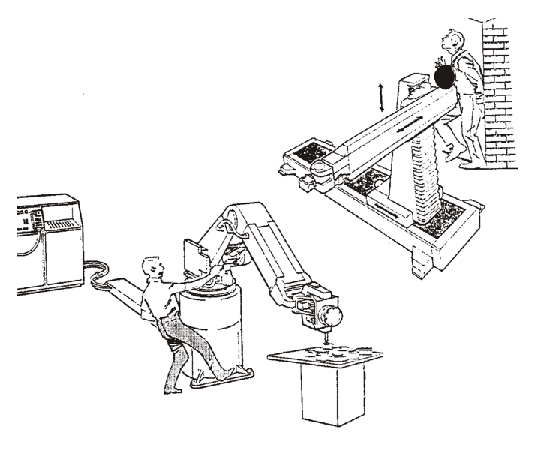
\includegraphics[draft=false]{nevarnosti.eps}}
\caption{\label{cop}Nevarnost trka in nevarnost stisnjenja pri
delu z industrijskimi roboti}
\end{figure}

Gornje nevarnosti izvirajo iz naslednjih vzrokov:
\begin{itemize}
    \item \vspace*{-0.1cm} \textbf{Nevarnosti krmilnega sistema:} To
    so nevarnosti napak, ki se dogode v robotskem krmilniku, kot
    so npr. programske napake, napake zaradi interference signalov ter napake v
    hidravličnih, pnevmatskih ali električnih podsistemih povezanih z robotom.
    \item \vspace*{-0.1cm} \textbf{Mehanske nevarnosti:} V ta
    razred sodijo nevarnosti, ki so posledica mehanskih lastnosti
    obdelovancev ali orodij, ki jih prenaša robot. Te so npr. ostri
    robovi, večje mase ali nezastrte elektrode. Zaradi mehanskih
    napak lahko robotsko prijemalo nepredvideno izpusti
    obdelovanec. Vzroki mehanskih napak so prekomerna obremenitev,
    korozija, utrujanje materiala in pomanjkljivo vzdrževanje.
    \item \vspace*{-0.1cm} \textbf{Nevarnosti okolja:} Uporaba
    robotov lahko v določenih situacijah povzroči tudi tveganja iz
    okolja. Tovrsten primer so varilne robotske celice od katerih
    se širijo varilni plini, varilno iskrenje ter leteči delci.
    Podobno tveganje predstavljajo tudi prah, vlaga, ionizirajoče in neionizirajoče
    sevanje, laserski žarki, ultraviolična svetloba ter gorljivi in
    eksplozivni plini.
    \item \vspace*{-0.1cm} \textbf{Nevarnosti človeških napak:} V
    večini robotskih celic mora operater delati v bližini robota
    ali vstopati v njegov delovni prostor. V tem primeru je
    izpostavljen nevarnosti trka ali stisnjenja, ki lahko nastopi
    med programiranjem, učenjem gibanja, vzdrževanjem, ali delom v
    bližini robota npr. vlaganjem ali jemanjem obdelovancev iz
    celice. Slabo poznavanje opreme je glavni vzrok za človeške napake pri delu z roboti.
    \item \vspace*{-0.1cm} \textbf{Nevarnosti perifernih naprav:}
    V večini robotskih celic robot dela v povezavi s perifernimi
    enotami, kot so obdelovalni stroji, tekoči trakovi,
    obdelovalna orodja, stiskalnice, itd. Tovrstna oprema prav tako
    lahko predstavlja varnostno tveganje, če so nevarni deli v
    dosegu operaterja in niso zaščiteni z varnostnimi ograjami.
\end{itemize}

Poročila o nesrečah z industrijskimi roboti odkrivajo, da se
večino nesreč dogodi, ko operater vstopi v robotski delovni
prostor potem, ko se je robot predhodno ustavil ali se gibal
počasi, nenadoma pa se je začel gibati in hitro pospeševati.

\clearpage
\section{Zahteve in zagotavljanje varnosti pri delu z roboti}

 \vspace{5mm}

\textbf{Splošne zahteve za varno delovanje industrijske strojne
opreme} predvidevajo, da morajo biti vsi gibajoči se deli opreme,
vsak del prenosnih sistemov in vsak nevaren del varno zakriti.
Izjeme obstajajo v primerih, ko so ti deli v takšnem položaju ali so
takšne konstrukcije, da so že sami po sebi varni kot da bi bili
zakriti. Smernice za varno delovanje strojev so podane v direktivah
o strojih 98/37/EC in 2006/42/EC. Pri klasičnih strojih so nevarni
deli običajno vgrajeni v njegovi notranjosti. Delovanje strojev je
pod popolno kontrolo človeka in so zato vzroki nesreč večinoma
pripisani človeškemu faktorju. V nasprotju s stroji, pa je pri
robotski celici lahko potencialno nevarna širša okolica robota, ki
obsega celoten robotov delovni prostor, pa tudi bližnjo okolico v
primeru letečih delcev ali kosov. Zaradi tega je potrebno skrbno
preučiti do kod sega področje nevarnosti in tega ustrezno zaščititi.
Pri tem je pomembna analiza potencialnih nevarnosti, ki mora biti
izvedena na sistematični način. Standard, ki ureja varno delovanje
robotskih celic, je novejši standard ISO 10218 (ang. naslov: Robots
for industrial enviroments - Safety requirements). Standard ni
obvezujoč, saj daje le praktična priporočila za zagotavljanje
varnega delovanja. Robotska celica, ki je zgrajena gleda na
priporočila, hkrati ustreza tudi direktivi o strojih.


\subsection{Zagotavljanje varnosti na nivoju strojne opreme}

 \vspace{5mm}

 \textbf{Varnostna zaščita} se glede na priporočila standarda
 EN 954-1:1999 (ang. naslov: Safety of machinery, Safety-related parts of
 control systems, Part 1: General principles for design, ki je
 harmoniziran ISO 13849-1:1999) lahko izvaja na treh nivojih:

\begin{description}
       \item \textbf{Nivo 1} je nivo varovanja obsega celotne robotske
       celice. Običajno je varovanje izvedeno s fizičnim
       ograjevanjem s pomočjo kombinacije mehanskih ograj in vrat.
       Kot opcija so lahko uporabljene tudi naprave za zaznavanje prisotnosti
       ter zvočne in svetlobne opozorilne naprave, vendar le kot dodatek za zagotavljanje večje varnosti.
       \item \textbf{Nivo 2} vključuje nivo varovanja človeka, ki
       se nahaja v delovnem prostoru robota. Običajno je varovanje
       izvedeno s pomočjo senzornih naprav za zaznavanje
       prisotnosti človeka. Z razliko s predhodnim nivojem, kjer gre predvsem
       za ograjevanje, je v tem primeru poudarek na zaznavanju prisotnosti operaterja.
       \item \textbf{Nivo 3} je nivo varovanja človeka v
       neposredni bližini robota. Varovanje na tem nivoju se
       izvaja z zaznavanjem prisotnosti človeka ali ovir v bližini
       robota ali pa neposrednega stika z robotom ter posledično, s takojšnjo
       zaustavitvijo delovanja. Za ta namen so uporabljane naprave
       za merjenje položaja človeka in različni senzorji, kot so
       npr. senzorji sil in momentov ali kontaktni senzorji dotika.
\end{description}
V večini robotskih aplikacij je zahtevan vsaj en nivo varovanja.
Glede na oceno tveganja, pa je mogoče izvajati več nivojev
varovanja hkrati.

Spodnje slike prikazujejo več primerov prvega nivoja varovanja,
kjer operater praviloma ne vstopa v samo robotsko celico. Na sliki
\ref{level1a} je prikazano \textbf{fizično ograjevanje robotske
celice z ograjo z vrati}. Operater lahko vstopi v robotsko celico
samo v primeru, ko robot ni v obratovanju. če vstopi med
obratovanjem, stikalo na vratih izklopi delovanje. V drugem in
tretjem primeru sta delovni prostor operaterja in robota popolnoma
ločena. Vstavljanje obdelovancev in jemanje obdelavancev iz celice
je izvedeno preko rotirajoče mize (glej sliko \ref{level1b}) ali
pomičnih mehanizmov (glej sliko \ref{level1c}).
\begin{figure}[h]
\begin{minipage}[c]{0.5\columnwidth}
\centering
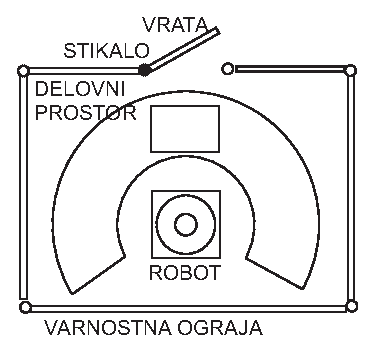
\includegraphics[width=0.60\columnwidth]{fence1.eps}
\end{minipage}
\begin{minipage}[c]{0.5\columnwidth}
\centering
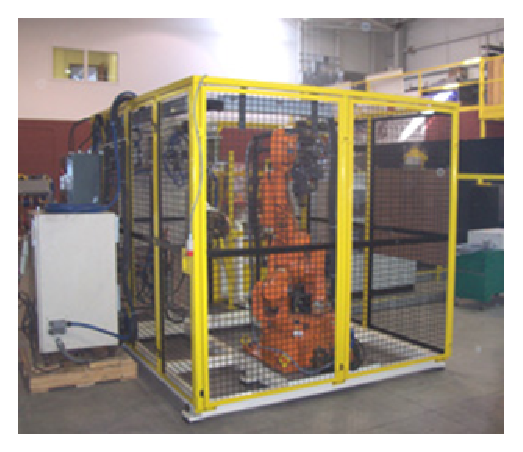
\includegraphics[width=0.9\columnwidth]{fence1_photo.eps}
\end{minipage}
\caption{\label{level1a}Prvi nivo varovanja s fizično ograjo in
vrati}
\end{figure}

\begin{figure}[h]
\begin{minipage}[c]{0.5\columnwidth}
\centering
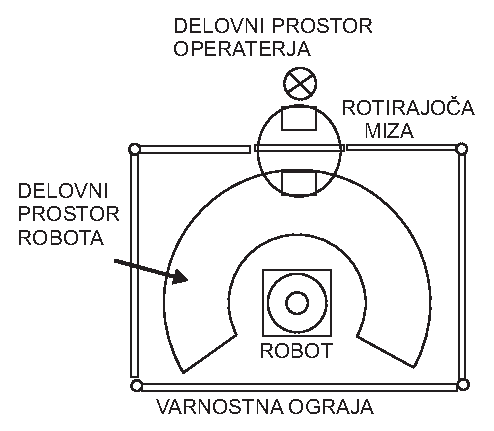
\includegraphics[width=0.80\columnwidth]{fence2.eps}
\end{minipage}
\begin{minipage}[c]{0.5\columnwidth}
\centering
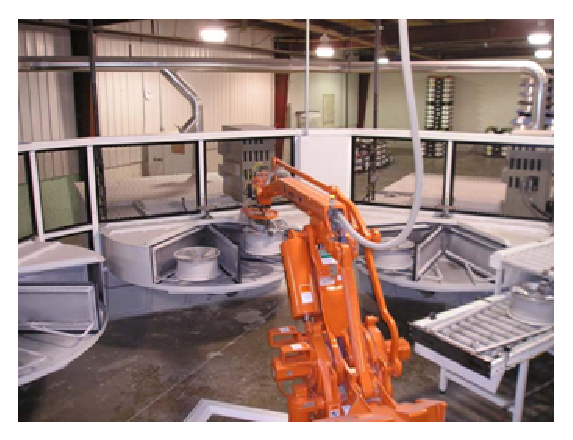
\includegraphics[width=0.9\columnwidth]{fence2_photo.eps}
\end{minipage}
\caption{\label{level1b}Prvi nivo varovanja s fizično ograjo in
rotirajočo mizo}
\end{figure}

\begin{figure}[h]
\begin{minipage}[c]{0.5\columnwidth}
\centering
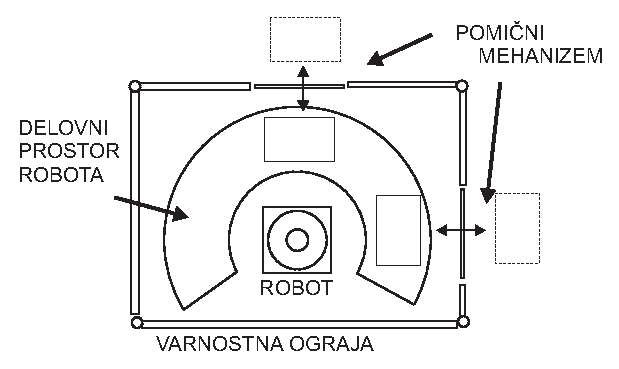
\includegraphics[width=0.90\columnwidth]{fence3.eps}
\end{minipage}
\begin{minipage}[c]{0.5\columnwidth}
\centering
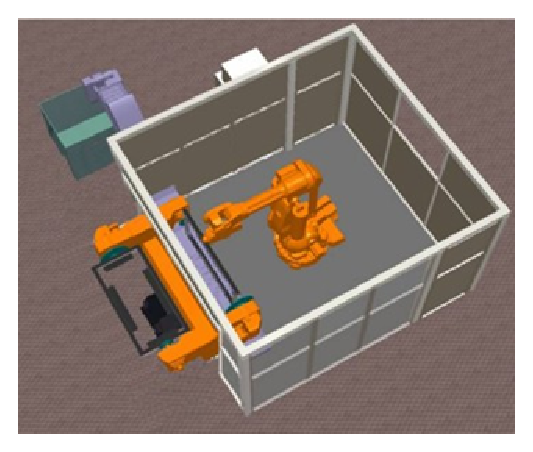
\includegraphics[width=0.9\columnwidth]{fence3_photo.eps}
\end{minipage}
\caption{\label{level1c}Prvi nivo varovanja s fizično ograjo in
pomičnimi mehanizmi}
\end{figure}

%\vspace{5mm}

Na drugem nivoju varovanja pri katerem operater lahko vstopa v
robotsko celico, je varovanje izvedeno na osnovi \textbf{senzorjev
za ugotavljanje prisotnosti operaterja}. To so običajno optični
senzorji, ki delujejo na principu zaznavanja prekinitve žarka,
postavljeni v formacijo optičnih zaves, kot je to prikazano na sliki
\ref{zavesa}. Alternativa je uporaba senzornih preprog, ki na osnovi
izmerjenega tlaka na podlago, zaznavajo položaj operaterja.
\begin{figure}[h]
\centering
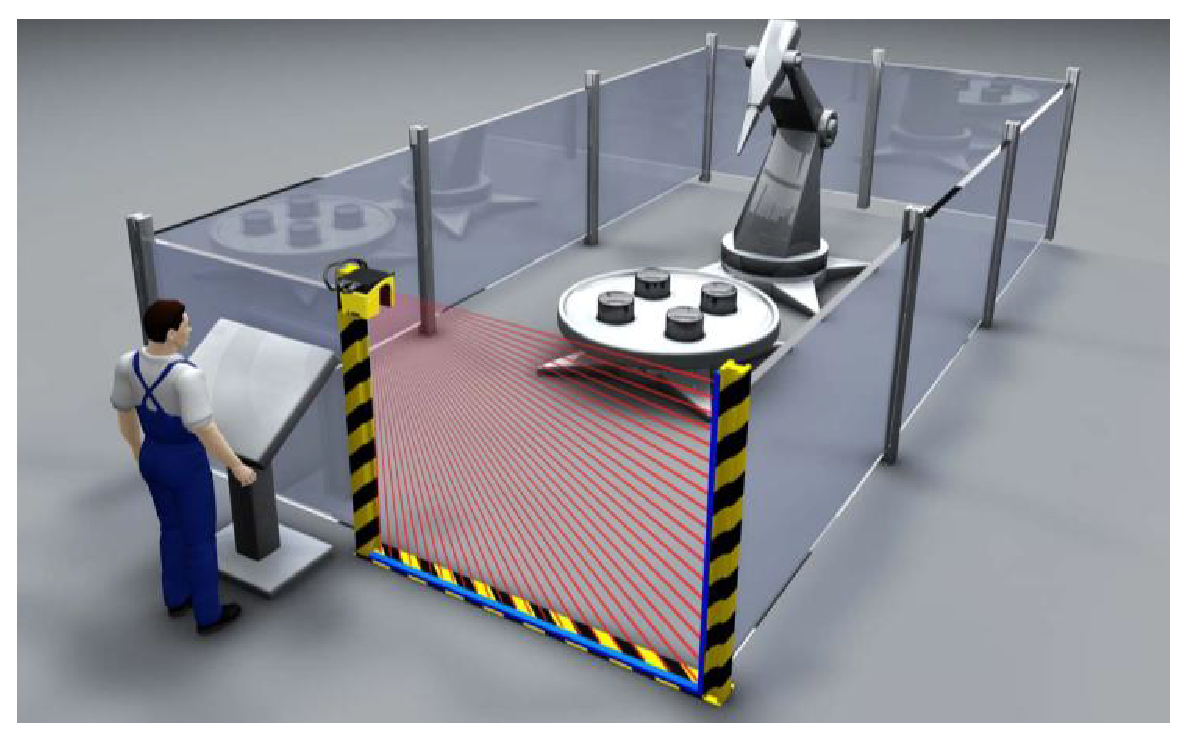
\includegraphics[width=0.7\columnwidth]{zavesa.eps}
\caption{\label{zavesa}Drugi nivo varovanja s pomočjo optičnega
senzorja za zaznavanje prisotnosti operaterja}
\end{figure}

V osnovi naj bi bili senzorji za ugotavljanje prisotnosti
uporabljeni le kot sekundarna oblika zagotavljanja varnosti in to le
v primerih, ko je nujno potreben omejen dostop do robota.

%\vspace{1mm}

Sodobni trendi uporabe robotskih sistemov se razvijajo v smeri
stalnega sodelovanja človeka in robota. Sistem varovanja mora
omogočati hitro prilagajanje robotske celice novim aplikacijam.
Fizično varovanje z mehanskimi ovirami se spreminja v elektronsko
varovanje. Tako so ključni element za zagotavljanje varnosti na
tretjem nivoju senzorji za zaznavanje objektov v delovnem prostoru
robota. Razvijajo se novi optični senzorji, kot so umetni vid in
laserski skenerji. Na sliki \ref{laser_scaner} je predstavljen
laserski skener, ki zaznava prisotnost objektov v različnih merilnih
območjih, s čimer je mogoče programsko določiti in zaznavati kdaj se
človek nahaja v varnem in kdaj v nevarnem območju robotske celice.
\begin{figure}[h]
\begin{minipage}[c]{0.4\columnwidth}
\centering
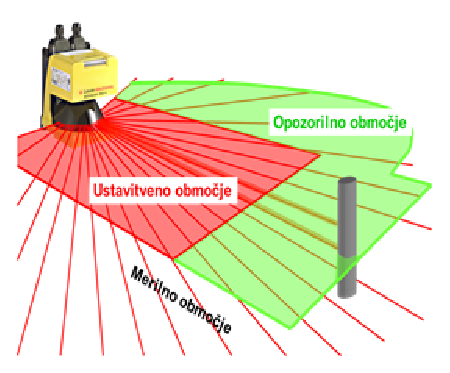
\includegraphics[width=0.98\columnwidth]{laser_scaner_obmocje.eps}
\end{minipage}
\begin{minipage}[c]{0.6\columnwidth}
\centering
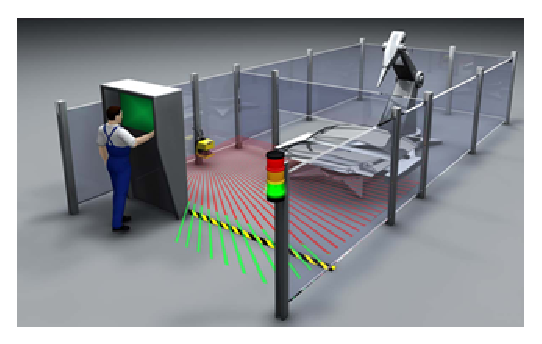
\includegraphics[width=0.98\columnwidth]{laser_scaner.eps}
\end{minipage}
\caption{\label{laser_scaner}Laserski skener za zaznavanje
prisotnosti operaterja s programabilnimi območji zaznavanja}
\end{figure}


\textbf{Senzorji za zaznavanje dotika z robotom} so nameščeni na
robotske segmente ali na vrh robota. Ta pristop se uporablja v
primerih celic z manjšimi roboti, kjer operater med obratovanjem
stoji v bližini robota. Signal, ki ponazarja dotik z robotom,
povzroči hipno izključitev obratovanja robotske celice.

\vspace{5mm}

\textbf{Tipka za izklop v sili} je pomembna pri zagotavljanju
varnosti, saj operaterju omogoča hitro zaustavitev gibanja robota.
Tipka za izklop v sili je nameščena na več mestih v robotski celici
in je nujno velika ter rdeče obarvana, da je lahko opazna in
dosegljiva. Praviloma je nameščena na robotskem krmilniku, na enoti
za ročno učenje ter na ograji robotske celice. Vse varnostne
naprave, kamor spada tudi tipka za izklop v sili, so zaradi čim
hitrejšega izklopa obratovanja s krmilnikom povezane preko ožičene
logike in niso del programske opreme. Sodobni roboti imajo že
vgrajene opcije elektronskega omejevanja gibanja osi (npr. ABB EPS)
ali omejevanja hitrosti gibanja robota ob prisotnosti človeka (npr.
ABB SafeMove).

\vspace{5mm}

Pomembne točke varnostnih priporočil standarda ISO 10218-1, ki
zadevajo nove rešitve varovanja so:
\begin{description}
    \item \vspace*{-0.1cm}5.9 - Priporočila za simultano delovanje več robotov,
    ki določajo pogoje za vodenje več robotskih manipulatorjev z enim krmilnikom.
    \item \vspace*{-0.1cm}5.10 - Zahteve in pogoji za skupno delovanje robota in človeka.
    \item \vspace*{-0.1cm}5.12.3 - Priporočila za programsko omejevanje gibanja
    osi in delovnega prostora, ki omogočajo uporabo elektronskih naprav in programskih
    orodij omejevanja delovnega prostora in hitrosti gibanja robota v smislu zagotavljanja varnosti.
\end{description}
Nov standard ISO 10218-2 (ang. naslov Robots and robotic devices -
Safety requirements Part 2: Industrial robot system and
integration), ki je v pripravi, bo še podrobneje obravnaval
sodelovanje človeka in robota.

\vspace{10mm}

\subsection{Zagotavljanje varnosti pri razvoju programske opreme}

\vspace{5mm}

\textbf{Programiranje in učenje robotskega gibanja} se izvaja s
pomočjo ročnega vodenja robota preko položajev, ki jih robotski
krmilnik pomni in jih nato v avtomatskem načinu izvaja. Za ta
namen je uporabljena enota za ročno učenje. Možno je tudi učenje s
fizičnim vodenjem vrha robota vzdolž trajektorije gibanja, ki si
jo robotski krmilnik zapomni in izvaja. V obeh primerih se mora
operater med učenjem nahajati v robotski celici relativno blizu
robotu. Med učenjem je zato za zagotavljanje varnosti potrebno
biti pozoren na:
\begin{itemize}
    \item \vspace*{-0.1cm} Operater, ki robot uči, mora biti za to
    dobro usposobljen, mora biti seznanjen z vsemi nevarnostmi in
    mora upoštevati ukrepe za zagotavljanje varnosti.

    \item \vspace*{-0.1cm} Med učenjem gibanja se robot ne sme
    gibati z visokimi hitrostmi.

    \item \vspace*{-0.1cm} Operater mora imeti lahek in hiter dostop do tipke za
    izklop v sili.

    \item \vspace*{-0.1cm} Operater mora v vsakem trenutku stati
    na mestu kjer je majhna možnost, da ga robot stisne k fiksnim objektom
    v celici ali da ga poškoduje v primeru okvare.
    Hkrati pa mora poskrbeti, da ima dober pregled nad obratovanjem.

    \item \vspace*{-0.1cm} Priporočljivo je, da je pri učenju
    prisoten opazovalec, ki se nahaja izven delovnega področja
    robota, in ima dostop do takojšnjega izklopa v sili.

    \item \vspace*{-0.1cm} Kjer je to potrebno, mora operater nositi
    zaščitno opremo in zaščitno obleko. Zaščitna čelada je
    obvezna, če obstaja možnost poškodbe glave.

    \item \vspace*{-0.1cm} Ročna učna naprava mora biti takšna, da omogoča gibanje robota samo v primeru, ko operater
    drži posebno tipko.
\end{itemize}


\newpage
\subsection{Zagotavljanje varnosti v Laboratoriju za robotiko na FE Ljubljana}

\vspace{5mm} V Laboratoriju za robotiko in biomedicinsko tehniko
na Fakulteti za elektrotehniko je za varno delo z roboti
poskrbljeno na naslednji način:

\begin{itemize}
    \item \vspace*{-0.1cm} Meje delovnega prostora robotov so
    označene na tleh z rumeno/črnim trakom.

    \item \vspace*{-0.1cm} Operater, ki vstopa v delovni prostor
    mora obvezno nositi zaščitno čelado.

    \item \vspace*{-0.1cm} Na vidnih mestih v vsaki celici se
    nahajajo tipke za izklop v sili.

    \item \vspace*{-0.1cm}Pri poskusnem zagonu se v delovnem
    prostoru ne sme nahajati nihče.

\end{itemize}
           % varnost pri delu z roboti
% -*- TeX:SI -*-
% slovene sub-mode for spell check

%\Large\textbf
\chapter{{Kratek pregled programiranja v Matlabu}}

\vspace{-3.35cm}

\begin{mdframed}[backgroundcolor=green!20, shadow=true,roundcorner=8pt]
\vspace{-0.35cm}
\section{Cilji poglavja}
\begin{itemize}
\item spoznati se z osnovnimi načini programiranja v Matlabu, ki jih boste potrebovali pri opravljanju vaj
\end{itemize}
\end{mdframed}


\section{Uvod}

V tem poglavju bo podan kratek pregled čez bistvene ukaze, ki jih boste potrebovali pri opravljanju vaj iz Osnov robotike. MATLAB je okrajšava za MATrix LABoratory in je bil v prvi verziji razvit za enostaven dostop do programskih knjižnjic LINPACK (linear system package) in EISPACK (Eigen system package). Danes pa je MATLAB visoko zmogljivo orodje za izračune v znanosti in tehniki, vendar ostaja še vedno najbolj popularen ravno zaradi enostavnosti izvajanja operacij nad vektorji in matrikami.

\section{MATLAB kot kalkulator}

Sicer precej nenavadno, vendar pa večina študentov, ko morajo izračunati kot ali zmnožiti dve števili, kljub temu, da imajo nekje v ozadju odprt MATLAB, iz torbe še vedno potegne svoj elektronski kalkulator ali pa zažene aplikacijo na svojem telefonu. Kljub kompleksnosti je MATLAB zelo uporaben tudi kot kalkulator. Brez razlage bomo podali nekaj primerov za ogrevanje:

\begin{lstlisting} 
1+2*3 %vpisemo numericni izracun
ans =
     7
\end{lstlisting}



\begin{lstlisting}
x = 3+4*7
x =
    31
2*x
ans =
    62
    
\end{lstlisting}



\begin {table}[htb]
\caption{Osnovne aritmetične operacije}
\vspace{0.5cm}
%\begin{center}
\begin{tabular}{|c|l|}
\hline   + &  seštevanje \\
\hline   - &  odštevanje \\
\hline   * &  množenje \\
\hline   / &  deljenje \\
\hline
\end{tabular}
%\end{center} \vspace{1cm}
\end {table}

\section{Dokumentacija za posamezne ukaze}

Dokumentacija o ukazih je dostopna na več načinov. Poleg dokumentacije na internetu, ki je dostopna preko strani http://www.mathworks.com/help/matlab/, je najlažje do dokumentacije dostopati direktno iz ukaznega okna matlaba. Ukaz help izpiše opis ukaza direktno v matlab ukaznem oknu
\begin{lstlisting}
help sin
 sin    Sine of argument in radians.
    sin(X) is the sine of the elements of X.

    See also asin, sind.
    Overloaded methods:
       codistributed/sin
    Reference page in Help browser
       doc sin
\end{lstlisting}

Ukaz doc odpre pomoč, ki vsebuje bolj podroben opis ukaza in več primerov uporabe.

\begin{lstlisting}
doc sin
\end{lstlisting}

\begin {table}[htb]
\caption{Najpogostejše matematične funkcije}
\vspace{0.5cm}
%\begin{center}
\begin{tabular}{|l|l|l|l|} \hline
cos(x)	& kosinus	& abs(x)	& absolutna vrednost \\ \hline
sin(x)	& sinus	& sign(x)	& predznak \\ \hline
tan(x)	& tangens	& max(x)	& največja vrednost \\ \hline
acos(x)	& arkus kosinus	& min(x)	& najmanjša vrednost \\ \hline
asin(x)	& arkus sinus	& ceil(x)	& zaokroži navzgor \\ \hline
atan2(y,x)	& arkus tangens	& floor(x)	& zaokroži navzdol \\ \hline
exp(x)	& eksponentna funkcija	& round(x)	& zaokroži do najbližje cele številke \\ \hline
sqrt(x)	& kvadratni koren	& pi	& število pi \\ \hline
log(x)	& naravni logaritem	& Inf	& naskončno \\ \hline
log10(x)	& logaritem z bazo 10	& NaN	& Not a number \\ \hline
norm(x)	& dolžina vektorja	& sum(x)	& vsota elementov \\ \hline

\end{tabular}
%\end{center} \vspace{1cm}
\end {table}

\section{Izris signalov}

Signale izrišemo s pomočjo ukaza \verb"plot(x,y)" oziroma \verb"plot(y)".

\section{Delo z vektorji}

Vektorji so lahko v matlabu vrstični
\vspace{-0.5cm}
\begin{lstlisting}
a = [ 1 5 3 6 3 7 2 4]
\end{lstlisting}
\vspace{0.2cm}

ali pa stolpični
\vspace{-0.5cm}
\begin{lstlisting}
p = [-0.2; 1; 5]
\end{lstlisting}
\vspace{0.2cm}

Do elementa vektorja p, ne glede na to ali je vektor stolpični ali vrstični, dostopamo na sledeči način
\vspace{-0.5cm}
\begin{lstlisting}
p(st_elementa)
\end{lstlisting}
\vspace{0.2cm}

Dolžino vektorja ugotovimo z ukazom length
\vspace{-0.5cm}
\begin{lstlisting}
length(p)
\end{lstlisting}
\vspace{0.2cm}

\section{Delo z matrikami}
Do vrstice matrike dostopamo na sledeči način
\vspace{-0.5cm}
\begin{lstlisting}
H(st_vrstice,:)
\end{lstlisting}
\vspace{0.2cm}

Primer: dostopanje do druge vrstice

\vspace{-0.5cm}
\begin{lstlisting}
H(2,:)
\end{lstlisting}
\vspace{0.2cm}


Do stolpca matrike dostopamo
\vspace{-0.5cm}
\begin{lstlisting}
H(:,st_stolpca)
\end{lstlisting}
\vspace{0.2cm}

Primer: dostopanje do tretjega stolpca
\vspace{-0.5cm}
\begin{lstlisting}
H(:,3)
\end{lstlisting}
\vspace{0.2cm}

Do elementa matrike dostopamo
\vspace{-0.5cm}
\begin{lstlisting}
H(st_vrstice, st_stolpca)
\end{lstlisting}
\vspace{0.2cm}

Primer: do elementa v tretji vrstici in drugem stolpcu dostopamo
\vspace{-0.5cm}
\begin{lstlisting}
H(3, 2)
\end{lstlisting}
\vspace{0.2cm}

\subsection{Ustvarjanje homogenih transformacijskih matrik}
Poglejmo kako ustvarimo homogeno transformacijsko matriko, ki je sestavljena iz rotacijskega in pozicijskega dela.
Ustvarimo enotsko matriko velikosti $4$
\vspace{-0.5cm}
\begin{lstlisting}
H = eye(4)
\end{lstlisting}
\vspace{0.2cm}

Ustvarimo 3x3 rotacijsko matriko rotacije okoli z osi
\vspace{-0.5cm}
\begin{lstlisting}
alpha = 1
R = [cos(alpha) -sin(alpha) 0; ...
     sin(alpha)  cos(alpha) 0; ...
              0           0 1]
\end{lstlisting}
\vspace{0.2cm}


Sedaj lahko matriko R zapišemo v matriko H
\vspace{-0.5cm}
\begin{lstlisting}
H(1:3,1:3) = R
\end{lstlisting}
\vspace{0.2cm}


Ustvarimo stolpični vektor p
\vspace{-0.5cm}
\begin{lstlisting}
p = [0.2; 0.15; -0.1]
\end{lstlisting}
\vspace{0.2cm}


Zapišemo stolpčni vektor v matriko H
\vspace{-0.5cm}
\begin{lstlisting}
H(1:3,4) = p
\end{lstlisting}
\vspace{0.2cm}


Alternativa zgornjemu zapisu je tudi
\vspace{-0.5cm}
\begin{lstlisting}
H = [R,p;[0 0 0 1]]
\end{lstlisting}
\vspace{0.2cm}

\subsection{Nekater funkcije za delo z matrikami}

Matriko ali vektor transponiramo z
\vspace{-0.5cm}
\begin{lstlisting}
R'
\end{lstlisting}
\vspace{0.2cm}

ali
\vspace{-0.5cm}
\begin{lstlisting}
transpose(R)
\end{lstlisting}
\vspace{0.2cm}


Inverz matrike izračunamo z ukazom \verb"inv"
\vspace{-0.5cm}
\begin{lstlisting}
inv(H)
\end{lstlisting}
\vspace{0.2cm}


Velikost matrike ugotovimo z ukazom \verb"size"
\vspace{-0.5cm}
\begin{lstlisting}
size(H)
\end{lstlisting}
\vspace{0.2cm}

Število vrstic matrike
\vspace{-0.5cm}
\begin{lstlisting}
size(H, 1)
\end{lstlisting}
\vspace{0.2cm}

Število stolpcev matrike
\vspace{-0.5cm}
\begin{lstlisting}
size(H, 2)
\end{lstlisting}
\vspace{0.2cm}

\section{Zanke in pogojni stavki}
\subsection{for zanka}
Primer for zanke, ki v vektor velikosti 12 zapisuje vrednosti
\vspace{-0.5cm}
\begin{lstlisting}
for i=1:12
	p(i) = (i-1)*3;
end
\end{lstlisting}
\vspace{0.2cm}


Primer for zanke, ki v matriko velikosti A 5x7 zapisuje vrednosti
\vspace{-0.5cm}
\begin{lstlisting}
for i = 1:5
    for j = 1:7
	   A(i,j) = j+(i-1)*5;
    end
end
\end{lstlisting}
\vspace{0.2cm}


\subsection{while zanka}

Primer while zanke, ki teče dokler je spremenljivka manjša od a. Ko spremenljivka a postane enaka ali večja od b se zanka ustavi in program teče dalje.
\vspace{-0.5cm}
\begin{lstlisting}
while (a<b)
	%razlicne operacije z vrednostima a in b
end
\end{lstlisting}
\vspace{0.2cm}

\subsection{if stavek}

\vspace{-0.5cm}
\begin{lstlisting}
if (pogoj)

end
\end{lstlisting}
\vspace{0.2cm}

Primer stavka, ki preveri, če ima vektor a dolžino tri, če je pogoj izpolnjen potem prvemu elementu vektorja a priredi vrednost 0.
\vspace{-0.5cm}
\begin{lstlisting}
if (length(a) == 3)
	a(1) = 0;
end
\end{lstlisting}
\vspace{0.2cm}


\subsection{if-else stavek}

\vspace{-0.5cm}
\begin{lstlisting}
if (pogoj1)

elseif (pogoj2)

elseif (pogoj3)

else

end
\end{lstlisting}
\vspace{0.2cm}







			


% -*- TeX:SI -*-
% slovene sub-mode for spell check
%%%%%%%%%%%%%%%%%%%%%%%%%%%%%%%%%%%%%%%%%%
% Glavni text
%%%%%%%%%%%%%%%%%%%%%%%%%%%%%%%%%%%%%%

\chapter[ABB RobotStudio]{Doma\v ca naloga \newline Programski paket za robotsko \newline simulacijo ABB RobotStudio}

\begin{mdframed}[backgroundcolor=green!20, shadow=true,roundcorner=8pt]
\vspace{-0.35cm}
\section{Cilji vaje}
\begin{itemize}
\item spoznavanje dela z off-line okoljem za programiranje robotov ABB
\item umestitev robota in CAD delovnih objektov  v navidezno okolje
\item uporaba novega vrha robota v obliki novega CAD orodja
\item definiranje uporabniških koordinatnih sistemov, ki pripadajo obdelovancu
\item uporaba ukazov za linearno in krožno premikanje robota po obliki obdelovanca
\item priprava programa za vodenje robota v navideznem okolju s pomočjo točk definiranih z modelom obdelovanca
\item simulacija izvajanja programa v navideznem okolju
\item prenos programa iz navideznega okolja na realni robot ABB

\end{itemize}
\end{mdframed}

\section{Uvod}
\emph{ABB RobotStudio} je simulacijski programski paket, ki omogoča grafično
prostorsko simulacijo delovanja robotskih celic. Programski paket omogoča:

\begin{itemize}
\item\vspace*{-0.35cm} prostorsko modeliranje robotske celice, ki
lahko vključuje več robotov hkrati, periferijo ter ostale naprave v
celici. Model robota vključuje kinematični model robota, ki omogoča
vodenje v zunanjih in v notranjih koordinatah, kakor tudi model
programskega jezika in okolja krmilnika. \item\vspace*{-0.35cm}
načrtovanje trajektorij gibanja (pri načrtovanju poti je v primerjavi
z realnim sistemom dobrodošla možnost načrtovanja glede na geometrijo
predmetov v celici), \item\vspace*{-0.35cm} simulacijo delovanja,
\item\vspace*{-0.35cm} kreiranje robotskega programa.
\end{itemize} Namen in prednosti uporabe robotske simulacije
so:
\begin{itemize}
\item\vspace*{-0.35cm} Vizualizacija ideje o avtomatizaciji določene
delovne naloge. \item\vspace*{-0.35cm} Preverjanje ustreznosti
različnih tipov robotov še pred odločitvijo o nakupu, kar omogoča
knjižnica modelov robotov. \item\vspace*{-0.35cm} Off-line
programiranje: Robotski program se v tem primeru razvije na
simulacijskem paketu na modelu celice, za prenos na realno celico v
proizvodnji pa je potreben le minimalen čas zaustavitve.
\end{itemize}

\vspace{15mm}

{\bf Zagon programskega paketa RobotStudio:}

\noindent Robot studio zaženite s klikom na ikonco v namizju ali
pod
\newline \textit{Start>Programs>ABB Industrial IT>Robotics IT>Robot
Studio}

\newpage
\section{Delovno okolje RobotStudio}

Izbira pogleda v delovnem okolju:
\begin{itemize}
\item\vspace*{-0.35cm} kolešček miške: približevanje/oddaljevanje
(zoom in/zoom out)

\item \vspace*{-0.35cm} srednja tipka miške (STM) + desna tipka miške
(DTM): rotacija točke pogleda

\item \vspace*{-0.35cm} tipka Control + leva tipka miške (LTM):
translacijski pomik točke pogleda.
\end{itemize}

\noindent Izbira objektov: krivulja, površina, objekt, skupina
objektov, ...

\noindent Lovljenje kurzorja na: mreži, v centru, v sredini med
oglišči, na oglišču, na robu \newline (enako z \textit{View>Snap
Mode})
\newline Ob hkratnem držanju tipke \textit{Alt} se prikazuje
trenutna izbira.


\begin{figure}[h]
\centering
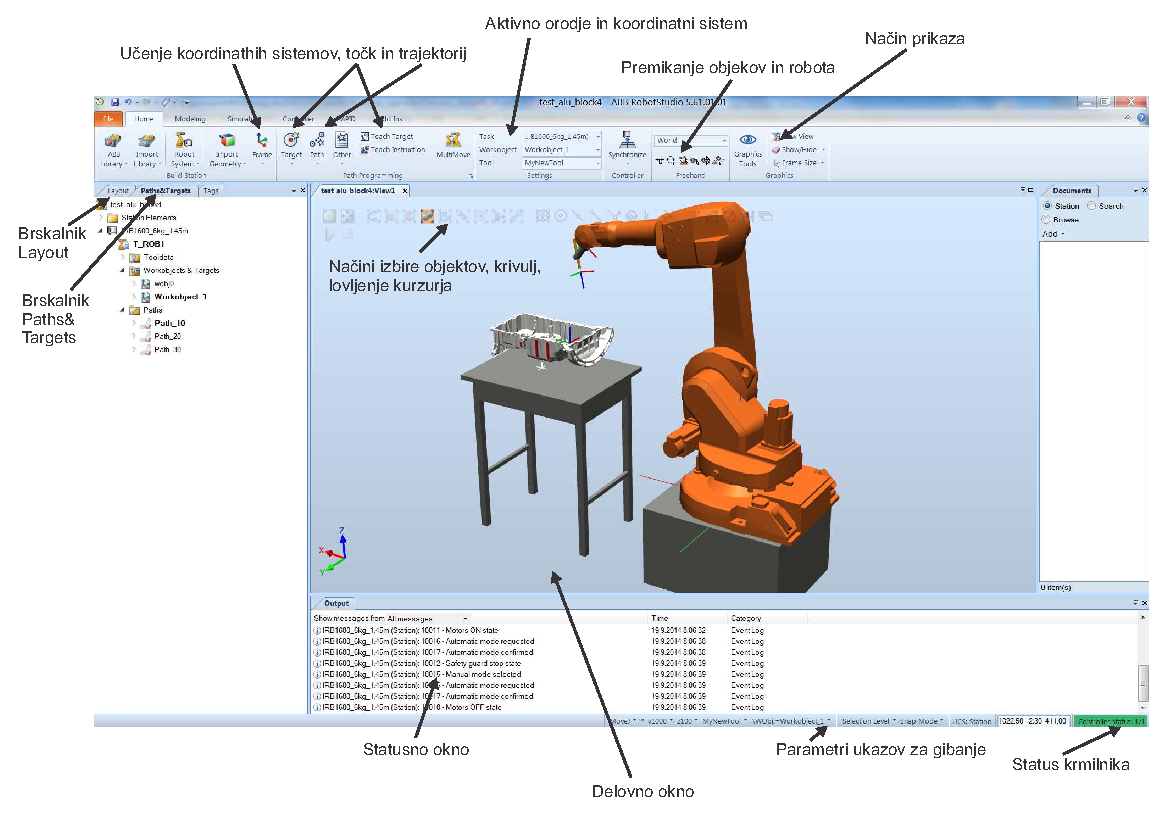
\includegraphics[width=1.0\columnwidth]{Delovno_okoljeRS_v6.eps}
  \caption{\label{figure1} Delovno okolje simulacijskega paketa RobotStudio}
\end{figure}


\newpage
\section{Načrtanje simulacijskega modela robotske celice}

Ustvari lokalno mapo \emph{D:$\setminus$Vaje$\setminus$or$\setminus$RobotStudio$\setminus$ImePriimek} (pri tem predlagamo, da namesto \v sumnikov uporabite \v crke brez stre\v sic). V lokalno mapo skopirajte zip datoteko \emph{PERIFERIJA.zip} iz mape \newline \emph{S:$\setminus$or$\setminus$RobotStudio$\setminus$PERIFERIJA} in jo odpakirajte. V datoteli se nahajajo robotska postaja, ki vsebuje robota, ki je enak realnemu robotu v laboratoriju LRBT (\emph{IRB1600 6kg 1.45m}) na podstavku in 3d modeli komponent, ki jih boste vklju\v cili v robotsko celico. To bo va\v sa lokalna kopija datotek, ki jih potrebujete za doma\v co nalogo. Odprite RobotStudio, v \emph{File} zavihku izberite  \emph{Open}, ter odprete  \emph{IRB1600.rspag} datoteko. Odpre se okno \emph{Unpack} \& \emph{Work}, kliknite \emph{Next}. Nato v \emph{Target folder} izberete va\v so mapo \emph{D:$\setminus$Vaje$\setminus$or$\setminus$RobotStudio$\setminus$ImePriimek} in izberete \emph{Next}. V naslednjem oknu ponovno izberete \emph{Next} in nazadnje \emph{Finish}. Sedaj po\v cakate, da se RobotStudio Package odpakira, ko lahko izberet \emph{Close}. Sedaj se odpre delovni prostor z robotom IRB\_1600\_6kg\_1.45m. Nadaljujete z ustvarjanjem orodja.

Sedaj lahko shranite postajo \emph{File>Save Station}. Postajo vam bo shranilo pod format datoteke \emph{rsstn}. To datoteko boste lahko urejali le na istem ra\v cunalniku, saj se v to datoteko na shranijo vse knji\v znjice, ki jih sicer potrebujete za odpiranje postaje na drugem ra\v cunalniku. \v Ce \v zelite postajo prenesti na drug ra\v cunalnik, je potrebno postaja prej NUJNO zapakirati. V \emph{File} zavihku izberete \emph{Share}, nato pa \emph{Pack and Go}. Postajo vam bo shranilo v \emph{rspag} datoteko, ki jo lahko preneste na drug ra\v cunalnik. Ko boste doma kon\v cali doma\v co nalogo jo morate nujno shraniti s \emph{Pack and Go}, sicer je ne bomo morali v laboratoriju, ko nam boste doma\v co nalogo \v zeleli predstaviti, odpakirati in pregledati.

\noindent \textbf{Kreirajte orodje} robota.
\begin{enumerate}
	\item Najprej naložite geometrijski model
	orodja preko \emph{Modelling>Import Geometry>Browse for Geometry...} - izberite \emph{orodje3.sat}.
	\begin{description} \item (Objekt se po
		vključitvi nahaja pod robotom in zato ni viden. \textbf{POZOR! Predno ga premikate oz.
			izvlečete izpod robota, ga obvezno definirajte kot orodje.} Torej nadaljujte z naslednjim korakom.)
	\end{description}
	\item Nato geometrijski model definirate kot orodje: \emph{Modelling>Mechanism>CreateTool} (zavihek \emph{Modelling}, orodno polje \emph{Mechanism}, ikona \emph{CreateTool}).
	\begin{itemize}
		\item izberite opcijo \emph{Use Existing} in izberite
		\emph{orodje3},
		\item vnesite položaj težišča: (-1.27, -1.27, 39.35) mm, maso 1 kg, vztrajnostni moment lahko izberete poljubno (recimo 0.1, 0.1, 0.1), \textbf{POZOR! RobotStudio razlo\v cuje med znakom za piko . in znakom za vejico , pri zapisu decimalnih \v stevil } zato je potrebno na nekaterih ra\v cunalnikih uporabiti za decimalni zapis pike, na drugih pa vejice. \v Ce vam torej ne uspe ustvariti orodja, je morda vzrok, da ste uporabili napa\v cni znak za zapis decimalnih \v stevil. Na novo odpakirajte \emph{PERIFERIJA.zip} in odprite popolnoma sve\v zo kopijo postaje.
		\item v naslednjem oknu določite vrh orodja tj. \emph{Tool Center Point} ali TCP, ki je določen glede na koordinatni sistem orodja. Vnesete koordinate (55.53, 0, 116.21) in rotacijo $50^o$ okoli osi \emph{y}. 
		\item Definirano točko dodate v spisek točk s pušcico v desno in zaključite.
		%    \item \vspace*{-0.cm} \hspace{0.5cm}- definicijo orodja je možno popravljati v brskalniku \newline \emph{Layout>Celica>MyNewTool DTM>ModifyToolData},
		\item definirano orodje pripnite na robot: v zavihku \emph{Layout} z miško primite
		\emph{MyNewTool} in ga povlecite na objekt $IRB1600\_6\_\_145\_01$. Odgovorite pozitivno na vprašanje ali želite posodobiti trenutno pozicijo, s čimer je orodje pripeto na zadnjem robotskem segmentu.
		%  \item \vspace*{-0.cm} \hspace{0.5cm}- orodje še pravilno orientirajte in sicer tako, da ga pod Elements izberete in z \emph{DTM>Rotate} orodje zavrtite za $180^o$ okoli $z$ osi lokalnega koordinatnega sistema.
	\end{itemize}
\end{enumerate}

Načrtan model robotske celice shranite.

%če sistema niste shranili, potem nadaljujte z navodili na strani \pageref{Prazna stran}. Sicer pa vedno lahko shranite sistem in nadaljujete z %navodili od tukaj naprej.

\noindent V prostor robotske celice \textbf{dodajte mizo} na katero bo postavljen obdelovanec preko \emph{Modelling>Import Geometry>Browse for Geometry...} - v mapi \newline
\emph{D:$\setminus$vaje$\setminus$or$\setminus$RobotStudio$\setminus$PERIFERIJA}
%\emph{(oz.//robo/student/or/RobotStudio/PERIFERIJA)}
izberite \emph{miza.sat}.
\begin{itemize}
\item  miza se znajde na ravnini
nič robotskega krmilnika, zato jo premaknite na 0 mm: v
zavihku \emph{Layout} na levi strani izberite mizo in z desno
tipko na miški (DTM) izberite \emph{Poisiton>Set Position}, z = -370 mm,
\item mizo premaknete po x na \emph{800 mm},
\item mizo zavrtite po z osi \textbf{lokalnega koordinatnega sistema} (\emph{Reference>Local}) za \emph{90 stopinj}.
\end{itemize}

Na mizo namestite obdelovanca:
\begin{itemize}
\item  v primeru uvoda odprite \textbf{kocko} (\emph{kocka.sat}). Kocka bo na višini \emph{483.5 mm} in premaknjena po x na \emph{960 mm} poravnana z ravnino mize.
\item ko boste delali doma?o nalogo pa na mizo namestite \textbf{aluminijasti blok} (\emph{alu\_blok.sat}). Postavite ga na pozicijo \emph{x=910, y=-40, z=570 mm}, ter zavrtite v oseh \textbf{lokalnega koordinatnega sistema} (\emph{Reference>Local}) \emph{x=90, y=0, z=180 stopinj}.
\end{itemize}


%\newline

\noindent Objekte v celici lahko premikate na več načinov: v
zavihku \emph{Layout} izberite objekt, ki se nahaja pod \emph{Components} in nato:
\begin{itemize}
   \item  objekt premikate s pomočjo ikonc \emph{Move} in \emph{Rotate} (ki se nahajajo v zavihku \emph{Home} v orodnem polju \emph{Freehand}) ter puščic, ali
    \item  objekt premikate tako, da v brskalniku izberete \emph{DTM>Set Position, >Rotate} ali >\emph{Place}
\end{itemize}




\section{Ročno vodenje robota}

Robot lahko ročno vodite na več načinov:

\begin{enumerate}
\item \vspace*{-0.2cm} Preko orodnega menija \emph{Freehand} z
\emph{Jog Joint}, \emph{Jog Linear} ali \emph{JogReorient} in robot
premikate z uporabo puščic.

%\item \vspace*{-0.2cm} Isto funkcionalnost kot pri 1 dosežete
%preko \emph{Jog Reorient} ali \emph{Jog Linear} ikonc.

\item \vspace*{-0.2cm}  V zavihku \emph{Layout} izberete robot
\emph{IRB1600\_5\_145\_\_01} in z \emph{DTM} izberete
\emph{Mechanism Joint Jog} ali \emph{Mechanism Linear Jog}. V teh
dveh načinih lahko ročno vnašate želene koordinate ali premikate
robot po korakih.

\end{enumerate}


\textbf{Naloga:} preizkusite vse možne načine ročnega vodenja!

\section{Kreiranje uporabniškega koordinatnega sistema (ang. Work object)}

Uporabniški koordinatni sistem oz. delovni objekt, ki je v bistvu koordinatni
sistem pripet na določen objekt, kreiramo z namenom, da točke gibanja učimo
relativno glede na ta objekt.  V primeru, da se objekt premakne, ostanejo
naučene trajektorije gibanja relativno glede na objekt enake.
\newline

\noindent Delovni objekt kreiramo tako, da najprej kreiramo koordinatni sistem
in sicer s pomočjo orodne ikonce \emph{Frame>Frame from Three Points} (nahaja se v orodnem polju \emph{Create}) s čimer
se odpre okno \emph{Create Frame}:
\begin{description}
\item \vspace*{-0.2cm} - izberemo opcijo Three Point, ki omogoča
definicijo koordinatnega sistem s tremi točkami. Prva točka
predstavlja izhodišče, druga določa smer $x$ osi, tretja pa smer $y$
osi. Kadar definiramo lego koordinatnega sistema glede na nek objekt
je najprimerneje, da koordinate točk določimo v t.i. \emph{Snap}
načinu:
\begin{itemize}
    \item \vspace*{-0.2cm} kurzor postavimo v okno za vpis koordinat točke,
    \item \vspace*{-0.2cm} v delovnem oknu izberemo
    način lovljenja koordinat v ogljiščih objekta \emph{Snap End},
\item \vspace*{-0.2cm} z držanjem tipke \emph{Alt} dobimo prikaz
lovljenja kurzorja glede na objekt,
    \item \vspace*{-0.2cm} z miško izberemo želeno ogljišče in koordinate se zapišejo v okno za definicijo koordinatnega sistema.
\end{itemize}

\item \vspace*{-0.2cm} - ko določimo koordinate vseh treh točk,
zaključimo definicijo koordinatnega sistema s \emph{Create} in dobimo
izrisan nov koordinatni sistem.

\item \vspace*{-0.2cm} - koordinatni sistem pretvorimo v delovni
objekt \emph{Workobject} z izbiro imena koordinatnega sistema v
zavihku \emph{Layout} ter z izbiro \emph{DTM>Convert Frame to
Workobject}

\item \vspace*{-0.2cm} - ustvarjen delovni objekt se znajde v
zavihku \emph{Paths\&Targets}

\item delovni objekt bomo sedaj povezali z objektom kocka. S tem se bo ob premikanju objekta kocka, s kocko ustrezno premikal tudi delovni objekt. V zavihku \emph{Paths\&Targets} z izbiro \emph{DTM>Attach to} odprete okno v katerem izberete objekt \emph{kocka} in negativno odgovorite na vprašanje, če želite posodibiti trenutno pozicijo.
\end{description}

\begin{figure}[h]
\centering\label{fig:kocka}
\includegraphics[width=0.7\columnwidth]{RStudio_workobject.eps}
  \caption{ Uporabniška koordinatna sistema na robu mize in robu kocke}
\end{figure}


\noindent Delovni objekt lahko tudi direktno kreiramo pod zavihkom \emph{Home} s klikom na ikono \emph{Other}
in \emph{Create Workobject}:
\begin{description}
\item \vspace*{-0.2cm} - delovni objekt poljubno poimenujemo ali
pustimo nespremenjeno,

\item \vspace*{-0.2cm} - opcijo \emph{Robot holds workobject}
izberemo \emph{False},

\item \vspace*{-0.2cm}- opcijo \emph{Moved by mechanical unit}
pustimo prazno,

\item \vspace*{-0.2cm}- opcijo \emph{Programmed} izberemo \emph{True}
(ker ne gre za premikajoči se koordinatni sistem), \item
\vspace*{-0.2cm} - določimo koordinatni system pod \emph{User Frame}:
\begin{itemize}
    \item \vspace*{-0.2cm} pozicijo in orinetacijo določimo tako, da izberemo izpis koordinat, kliknemo v eno, in nato v celici kliknemo na želeno točko (prej pravilno izberemo \emph{Snap
    mode}),
    \item \vspace*{-0.2cm} orientacijo koordinatnega sistema določimo ali z vnosom želenih zasukov ali pa z opcijo \emph{Frame by points}, kjer z izbiro treh točk določimo zasuk koordinatnega
    sistema,
    \item \vspace*{-0.2cm} izberemo \emph{Create} in dobimo izrisano nov koordinatnih
    sistem.
\end{itemize}
\end{description}


\noindent Delovni objekt lahko popravljamo tako, da ga v zavihku
\emph{Paths\&Targets} izberete in preko \emph{DTM>Modify Workobject}
popravite želene parametre.

\vspace{1cm}

\noindent \textbf{Naloga:} Pri uvodu v vajo določite delovni objekt na objektu z izhodiščem v enem od vogalov kot prikazuje slika \ref{fig:kocka}.

\begin{figure}[h]
\centering\label{fig:kalibSpice}
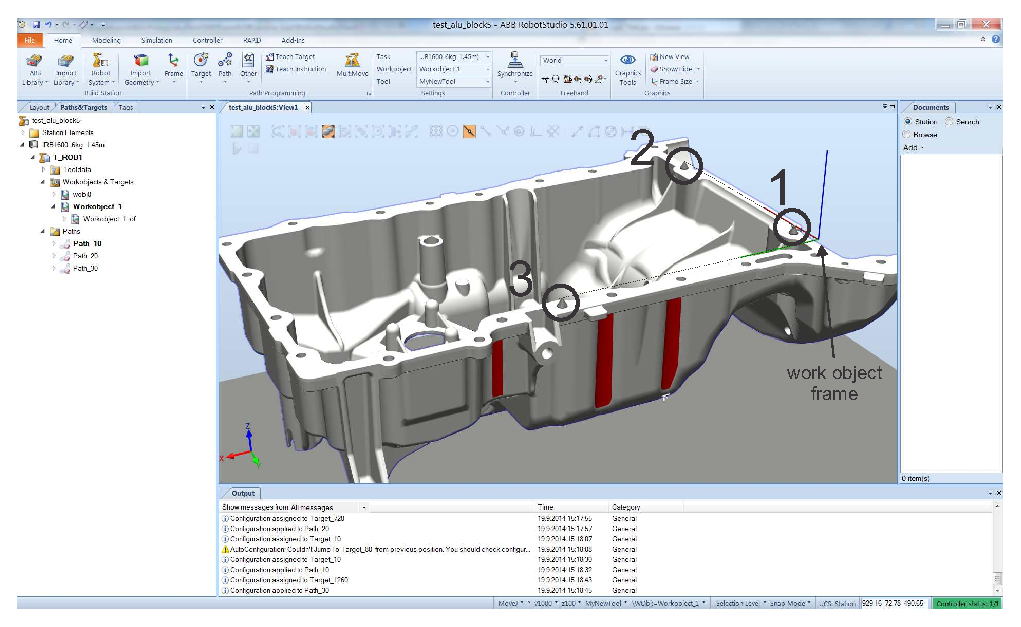
\includegraphics[width=0.9\columnwidth]{alu_blok_frame.eps}
  \caption{Uporabniška koordinatna sistema na modelu aluminijastega bloka.}
\end{figure}

Pri vaji pa postavite posamezne točke na kalibracijske špice, ki se nahajajo na modelu aluminijastega bloka kot prikazuje slika \ref{fig:kalibSpice}.

\comment{

\section{KREIRANJE UPORABIŠKEGA KOORDINATNEGA SISTEMA (User
Coordinate System - UCS)}

Uporabniški koordinatni sistem definiramo, kot poljubni koordinatni
sitem v prostoru. Uporaben je, če želimo določevati položaj točk ali
lego nekega objekta gleda nanj. Npr. če v zavihku \emph{Layout}
izberemo določen objekt in z \emph{DTM>Set as UCS} določimo
koordinatni sistem kot je koordinatni sistem tega objekta. Glede nanj
lahko določamo lego točk.

}

\section{Kreiranje ciljnih točk}

Ciljne točke (ang. Target points - TP) so lege vzdolž katerih se robot
giblje. Ciljne točke je možno kreirati na več načinov:

\begin{enumerate}
\item  Robot \textbf{ročno vodimo} v želen položaj z uporabo enega od
opisanih načinov in v želenem položaju izberemo ikono \emph{Teach
Target} (zavihek \emph{Home}, orodni meni \emph{Path Programming}). Na ta na?in u?imo to?ke, ki se ne nahajajo na obdelovancu. Vedno je potrebno robota pripeljati nad obdelovanca, zato da se robot brez trkov varno pribli?a obdelovancu. V tem primeru uporabimo tak na?in u?enja to?k. Robota ro?no prestavimo v neko to?ko nad obdelovancem od koder bo gibanje robota do obdelovanca varno. 

V zavihku \emph{Paths\&Targets} se pojavi nova točka v delovnem
objektu \emph{(Paths\&Targets>Workobject)}, ki je trenutno izbran kot
aktiven, kar pomeni, da so koordinate točke določene glede na ta
delovni objekt (ta trenutek lahko izbiramo med \emph{wobj0}, ki je
bazni ks in \emph{Workobject\_1}, ki je ks mize oz. objekta).

\item Lahko pa točke učimo \textbf{glede na geometrijo} objektov, ki
so prisotni v celici, in sicer:

\begin{itemize}
\item izberemo želen način lovljenja kurzorja (\emph{Snap mode}).
Namig: s hkratnim držanjem tipke \emph{Alt} vidimo ulovljen položaj
kurzorja.

\item točko - TCP kreiramo s \emph{Target>Create Target}, odpre se
nastavitveno okno:

\begin{description}
       \item - izberemo koordinatni sistem, glede na katerega definiramo točko
       \emph{Reference},
       \item - izberemo pozicijo, tako da kliknemo v koordinato in nato kliknemo na
       objekt,
       \item - orientacijo lahko ročno vpišemo ali jo popravljamo
       kasneje,
       \item - novo točko, ki se pojavi v delovnem objektu, kreiramo s
       \emph{Create},
\end{description}

       \item  nova točka, ki je določena preko geometrije nima določene konfiguracije robota, kar je potrebno naknadno določiti. (To se vidi v zavihku \emph{Paths\&Targets}, kjer se pri točki
       nahaja rumen trikotnik s klicajem)

    \item orientacijo orodja v naučeni točki preverimo tako, da v zavihku \emph{Paths\&Targets} izberemo točko in z \emph{DTM>View Tool at Target} dobimo prikaz lege orodja v točki. Vključimo tudi opcijo \emph{View Robot at Target} in s tem dobimo prikaz lege robota v točki.

    \item  orientacijo v naučeni točki  popravljamo z \emph{Paths\&Targets>DTM>Modify Target}, \emph{Rotate} ali ostale opcije, npr. \emph{Set Normal to Surface}, ali \emph{Align Target Orientation} z izbrano
    osjo (izbrana naj bo opcija \emph{Local} za koordinatni sistem).

    Orientacijo ni potrebno nastavljati za vsako točko posebej. Lahko jo kopiramo z ene točke s \emph{Copy orientation} in \emph{Apply orientation} v zavihku \emph{Paths\&Targets in
    DTM}.
%Lahko jo določimo samo nekaj točkam, vmesnim pa jo določi funkcija
%    \emph{Interpolate}.

    \item ko je nastavljena želena orientacijo, konfiguracijo robota določimo z \newline \emph{Paths\&Targets>izbrana točka>DTM>Jump to Target}. Izberemo želeno konfiguracijo in pri tem opazujemo notranje spremenljivke sklepov. Po potrditvi pri točki izgine trikotnik s klicajem.

\item Konfiguracijo se da določiti tudi za vse točke poti hkrati. Pod
\emph{Paths\&Targets>path>DTM} izberemo \emph{Auto Configuration}.
\end{itemize}
\end{enumerate}


\section{Načrtovanje trajektorije gibanja}

Trajektorijo gibanja (ang. path) načrtamo z naučenimi točkami ali s pomočjo
krivulj na geometrijskih objektih:

\begin{enumerate}

\item \vspace*{0.2cm} načrtanje trajektorije \textbf{s pomočjo
naučenih točk TCP}
\begin{itemize}
    \item izberemo orodno ikonco \emph{Empty Path}. Pod \emph{Paths\&Targets} se pojavi nova trajektorija.
    \item v statusni vrstici čisto spodaj desno izbiramo želen način gibanja npr. \emph{MoveJ} ali
    \emph{MoveL} ter ostale parametre instrukcij za gibanje
    \item instrukcije vrivamo z izbiro orodne ikonce \emph{Teach Instruction} ali pa točke TCP v zavihku \emph{Paths\&Targets} v pravilnem zaporedju kliknemo in jih povlečemo v trajektorijo.
    \item posamezne instrukcije za gibanje lahko popravljamo pod \emph{DTM>Modify Instruction}
\end{itemize}
\item \vspace*{0.2cm} načrtanje ukaza za gib \textbf{brez naučene
TCP}
    \begin{itemize}
    \item izberemo orodno ikonco \emph{Move Instruction} in vnesemo želene
koordinate položaja vrha robota
    \end{itemize}

\item \vspace*{0.2cm} načrtanje \textbf{krožnega gibanja}
\begin{itemize}
\item  za gibanje po krožnem loku morata biti na voljo začetna in
vmesna točka TCP \item kreiramo pot s \emph{Empty Path} in v pot
povlečemo točki, \item v zavihku \emph{Paths\&Targets} izberemo
hkrati oba ukaza za gib v točki in ju z \emph{DTM>Convert to Move
Circular} pretvorimo v ukaz krožni gib.
\end{itemize}

\item \vspace*{0.2cm} načrtanje \textbf{poti s pomočjo krivulj} na
geometrijskih objektih
\begin{enumerate}
    \item Najprej iz geometrije \textbf{ustvarimo krivuljo} in sicer v \emph{Home} načinu s pomočjo menija \emph{Path}. V tem meniju kreiramo pot brez točk (možnost \emph{Empty Path}) ali pot iz geometrije, kar nas v našem primeru zanima, ko izberemo \textbf{\emph{AutoPath}}.
        \item Ko izberete \emph{AutoPath} se odpre na levi strani meni z možnostimi za določanje krivulje. Držite tipko \textbf{Shift} in izberete rob na površini na bloku v glavnem oknu. Z odebeljeno rdečo črto se izriše možna krivulja, ki jo potrdite s klikom na DTM. Ko izberete krivuljo se v oknu na levi strani izpišejo robotvi od \emph{Edge\_1} naprej.
        \item Določite lahko tudi različne možnosti za krivuljo:
        \begin{itemize}
        \item \emph{Linear} - pot bo zgrajena iz samih ravnih odsekov z \emph{MoveL} ukazi.
        \item \emph{Circular} - program sam ugotovi, kateri del poti je primeren za interpolacijo s krožnim lokom in za ta del poti doda \emph{MoveC} ukaze.
        \item Možnosti \emph{Depart} in \emph{Approach} se odpreta, če gliknete na gumb \emph{More}. če v okna vpiše vrednost različno od nič, potem doda dodatno točko, ki je odmaknjena od krivulje. Možnost \emph{Approach} doda točko na začetku poti, možnost \emph{Depart} pa na koncu poti.
        \end{itemize}
        \item Z izbiro gumba \emph{Create} ustvarite pot, ki se pojavi v oknu \emph{Paths\&Targtes}, kjer jo lahko urejate naprej.


%\begin{enumerate}
%    \item najprej iz geometrije \textbf{ustvarimo krivuljo} in sicer v \emph{Modeling} načinu s pomočjo menija \emph{Curve}.
%        V tem meniju lahko kreiramo razne geometrijske oblike (ravno črto, krog, elipso, kvadrat,...)
%        ali uporabimo
%                \emph{Border arround Bodies} - krivulja, ki je meja med dvema objektoma, če sta v
%                dotiku\newline
%                \emph{Create Border Arround Surface} - krivulja okoli površine (izbira lovljenja kurzorja naj bo  površina (Surface))\newline
%            \emph{Create Border From Points} - krivulja, ki jo tvorijo točke
%
%         \item \textbf{krivuljo pretvorimo v pot} v meniju \emph{Home>Path From Curve} (pazite, da je  izbran želen način gibanja)
%        odpre se nastavitveno okno:
%            \begin{itemize}
%            \item s klikom izberemo krivuljo, ki jo želimo pretvoriti v pot
%            \item  izberemo opcijo \emph{Create on curve} \newline
%                - izberemo Delovni objekt (glede na katerega je pot določena) - \emph{Workobject\_1}
%             \item za \emph{Target Parameters} izbiramo:
%                \begin{description}
%                \item \emph{Approach(deg)} - orientacija okoli x osi
%                \item \emph{Travel} -    orientacija okoli y osi
%                \item \emph{Spin} -      orientacija okoli z osi
%                \item \emph{Approach} -  približevanje začetni točki na krivulji
%                \item \emph{Depart}  -   odmik od končne točke na krivulji
%                \item \emph{Local Target Offset} - odmik posamezne točke vzdolž krivulje
%                \end{description}
%            \item za \emph{Approximation Parameters} izbiramo:
%                \begin{description}
%                \item \emph{Max chord dev} - maksimalna dovoljena deviacija poti od
%                krivulje \newline
%                    Nižja izbrana toleranca pomeni več kreiranih ciljnih točk.
%                \item \emph{Line/circular} - linearna ali krožna interpolacija med točkami poti
%                \item \emph{Min dist} - minimalna reazdalje med točkami - velja samo za linearno interpolacijo
%                \item \emph{Max rad} - makismalni radij, ki velja za krožno interpolacijo med točkami.
%                \end{description}
%            \end{itemize}
 \end{enumerate}
\end{enumerate}
\vspace{0.3cm}
 \noindent Na ta način načrtane točke poti nimajo
določene orientacije in konfiguracije. Orientacijo lahko določimo
ročno preko menija \emph{Modify Target} ali orientacijo kopiramo iz
ostalih točk (\emph{Copy orientation} in \emph{Apply orientation}).
Konfiguracijo robota v točkah lahko ročno določimo za vsako točko
posebej (menija \emph{Jump to Target} ali \emph{Configuration}) ali
pa uporabimo meni \emph{Autoconfiguration} za celotno trajektorijo.

\vspace{0.3cm} \noindent Priporočljivo je, da načrtano pot tudi
interpoliramo z vmesnimi točkami, s čimer se izgonemo sporočilom o
napakah v zvezi s konfiguracijo robota (meni \emph{DTM>
Path>Interpolate Path}).

\vspace{0.3cm} \noindent Načrtano pot je mogoče rotirati ali translirati (v
zavihku \emph{Paths\&Targets} izberemo pot\emph{>DTM>Path}), ali pa obrniti
vrstni red izvajanja gibanja  (v zavihku \emph{Paths\&Targets} izberemo
pot>\emph{DTM>Modify Path>Reverse Path>Simple} ali \emph{Advanced}).

\vspace{0.3cm}
 \noindent \textbf{Naloga:} Načrtajte pot po
zunanjem in notranjem robu bloka ter pot po polkrogu na sprednjem delu bloka kot je prikazano na sliki \ref{fig:trajektorije}. Na \emph{S:$\setminus$or$\setminus$RobotStudio$\setminus$PERIFERIJA} se nahaja video simulacije \emph{RobotStudio.Wmv}, ki prikazuje pot gibanja robota.

\begin{figure}[h]
\centering
\includegraphics[width=1.0\columnwidth]{trajektorija.eps}
  \caption{\label{fig:trajektorije} Načrtana trajektorija po zunanjem robu modela bloka}
\end{figure}

\clearpage
\section{Preverjanje trkov z drugimi objekti}

Preverjanje trkov med posameznimi objekti (ang. Collision Detection) je možno
samo med simulacijo delovanja ali pa ves čas načrtovanja celice. Opcijo
vključimo na naslednji način: S \emph{Simulation>Create Collision Set}
ustvarimo dve množici objektov za kateri se bo preverjala kolizija. V
zavihku \emph{Layout} v množico \emph{ObjectsA} z miško povlečemo npr.
robot in orodje, v množico \emph{ObjectsB} pa ostale elemente v celici. Ob
koliziji objekti spremenijo barvo.

Z \emph{DTM>Modify Collision Set} izbiramo toleranco in barvo
obarvanja. Pod \emph{File>Options>Simulation>Collision} nastavljamo ostale nastavitve.


\section{Kreiranje robotskega programa}

Iz načrtanih trajektorij gibanja ustvarimo robotski program, ki vsebuje ukaze
programskega jezika RAPID, s postopkom \emph{sinhronizacije z virtualnim
krmilnikom}. Program sinhroniziramo preko menija \emph{RAPID>Sinhronize to
VC}. Opcija je tudi preko zavihku \emph{Paths\&Targets}, kjer izberemo
\emph{T\_ROB1} in z \emph{DTM>Sinhronize to VC}. Kreirani robotski program se
nahaja v zavihku \emph{Controller} ter \emph{RAPID>T\_ROB1>Module 1}.

\section{Simulacija izvajanja}

Izvajanje posameznih gibov lahko preverimo tako, da v zavihku
\emph{Paths\&Targets} izberemo posamezen segment in gib preverimo z
\emph{DTM>Execute Move Instruction}, izvajanje posamezne poti pa z
\emph{Move Along Path}

Izvajanje celotnega že sinhroniziranega robotskega programa pa
simuliramo s simulatorjem. Parametre simulacije nastavimo v meniju
\emph{Simulation>Simulation Setup}, tu v srednje okno povlečemo vse
želene poti, katerih gibanje želimo simulirati. Ustrezno izberemo
parameter \emph{Entry Point}. Izvajanje simulacije poženemo z izbiro
\emph{Simulation>Play}.

\section{Tekstovno urejanje robotskega programa}

Kreirane programske vrstice lahko vidimo in ročno urejamo s pomočjo
tekstovnega urejevalnika  \emph{RAPID Editor}. Program se nahaja v direktoriju z
imenom \emph{RAPID>T\_ROB1>Program Modules}.

%zahtevati dostop in sicer tako, da najprej zaženete \emph{Virtual
%FlexPendant}, potem zahtevate dostop v
%\emph{Elements>System11>DTM>Request Write Access}, ga v virtualnem
%flex pendantu potrdite in ga potrdite še v delovnem oknu z
%\emph{Enable Edit}.

\vspace{0.3cm} \noindent Spremembe v programu potrdite s tipko
\emph{Apply Changes}.

\vspace{0.3cm} \noindent Program lahko preizkušate v s pomočjo
vrivanja ustavitvenih točk in izvajanja po korakih.


\vspace{0.3cm} \noindent Program shranite v datoteko pod želenim
imenom tako, da v brskalniku izberete program in preko menija
\emph{Program>Save Program As} ali \emph{DTM>Save Program As}
shranite datoteko s končnico .pgf. Najbolje, da si program
shranite v svoj lasten direktorij.

\vspace{0.3cm} \noindent Na spodnji sliki je prikazano delovno okno
urejevalnika programa \emph{RAPID Editor}, z brskalnikom v levem
oknu, statusom aktivnega krmilnika v gornjem oknu in robotskimi ukazi
v desnem oknu.

\begin{figure}[h]
\centering
\includegraphics[width=0.9\columnwidth]{Delovno_okoljeRSOnline_v6.eps}
  \caption{\label{figure2} Delovno okolje urejevalnika programa RAPID Editor}
\end{figure}



\section{Izvedba naloge}

Naučite se osnovnega rokovanja s programskim paketom za simulacijo delovanja
robotskih sistemov \emph{ABB RobotStudio}: industrijskim robotom ABB IRB
1600-6/145. Pri uvajanju preizkusite:
\begin{itemize}
\item\vspace*{-0.25cm} Načrtajte model robotske celice, ki vključuje industrijski robot ABB IRB.
1600-6/145

\item\vspace*{-0.25cm} V model robotske celice vključite model
orodja za nanašanja lepila.

\item\vspace*{-0.25cm} V model robotske celice vključite model
obdelovanca (aluminijasti blok).

\item\vspace*{-0.25cm} Definirajte uporabniški koordinatni sistem na obdelovancu s pomočjo kalibracijskih špic, ki se nahajajo na obdelovancu.

\item\vspace*{-0.25cm} Načrtajte trajektorije gibanja po zunanjem in notranjem zgornjem robu bloka, ter po krožnem profilu na sprednjem delu bloka (glej sliko \ref{fig:trajektorije}). Trajektoriji na zgornjem robu naj bo sestavljena iz linearnih gibov (\emph{MoveL}), krožni gib za profil na sprednjem delu bloka pa naj bo sestavljen iz gibov za krožni lok (\emph{MoveC}). Na \emph{S:$\setminus$vaje$\setminus$or$\setminus$RobotStudio$\setminus$PERIFERIJA} se nahaja video simulacije \emph{RobotStudio.Wmv}, ki prikazuje pot gibanja robota.

\item\vspace*{-0.25cm} Izvedite simulirano nanašanje lepila v simulacijskem načinu
delovanja.

\item\vspace*{-0.25cm} Načrtane trajektorije gibanja pretvorite v robotski
program.

\item\vspace*{-0.25cm} Program shranite v ustrezno datoteko, da ga boste lahko preizkusili
na realnem sistemu v vaji 5.
\end{itemize}



%\pagebreak[4]
%
%Ta stran je namenoma prazna.

\label{Prazna stran}       % RobotStudio
\chapter{Manipulacija objektov z robotom Epson E2S651 in robotskim vidom} %
%\Large%
%\textbf{Cilj vaje} \\%
%\\%
%\normalsize%

\vspace{-3.5cm}

\begin{mdframed}[backgroundcolor=green!20, shadow=true,roundcorner=8pt]
\vspace{-0.35cm}
\section{Cilji vaje}
\begin{itemize}
\item spoznavanje uporabniškega okolja Epson RC+ za premikanje in programiranje robota Epson
\item spoznavanje ukazov za premikanje robota SCARA konfiguracije
\item sharnjevanje ciljnih točk robota
\item delo z I/O enoto
\item načina za definiranje palete
\item uporaba video sistema v kombinaciji s homogenimi transformacijami  za robotsko manipulacijo detektiranih objektov
\item spoznavanje okolja Matlab za namen preračuna homogenih transformacij
\item uporaba znanja pridobljenega na predavanjih o homogenih transformacijah med različnimi koordinatnimi sistemi
\end{itemize}
\end{mdframed}

\section{Pregled vaje}
\vspace{0.3cm}%
\underline{\textbf{1. del}} \\%

Na mizo v delovnem prostoru robota postavite zamašek in ga z robotom
oz. robotskim prijemalom primete. Prijetega odnesite nad poljubno
ustje plastenke in ga privijte.  Po krajšem premoru ga odvijte in
odnesite na začetno pozicijo. Tu ga spustite, robot pa umaknete.

\underline{\textbf{2. del}} \\%

Z uporabo robotskega vida in robota Epson E2S651 določite pozicijo
poljubno postavljenih zamaškov v delovnem prostoru robota (Slika
\ref{fScara_Del2}) in jih privijte na ustja plastenk. Pri nalogi je
potrebno izvesti postopek kalibracije s katero definirate lego
koordinatnega sistema kamere v referenčnem koordinatnem sistemu
robota. Za izračun potrebnih transformacij uporabite okolje Matlab,
za gibanje robota pa razvojno okolje Epson RC+.
%\psfull %

\begin{figure}[h]
    \centering
    \includegraphics[width=0.83\textwidth]{/Eps/000_Prvi_del.eps}
    \vspace{-0.3cm}
    \caption{Postavitev zamaškov v delovnem prostoru robota.}
    \label{fScara_Del2}
\end{figure}

\section{Lastnosti sistema}

Robot Epson E2S651 je robot tipa SCARA srednje velikosti. Njegove
najpomembnejše lastnosti kaže tabela na sliki \ref{fTabela}.

\begin{figure}[h]
    \centering
    \includegraphics[width=0.8\textwidth]{/Eps/01_Tabela.eps}
    \vspace{-0.3cm}
    \caption{Lastnosti robota Epson E2S651}
    \label{fTabela}
\end{figure}

Robot med delom v industrijskem proizvodnem procesu je prikazan na
sliki \ref{fRobot}, kjer je uporabljen kot nosilec laserskega
triangulacijskega merilnika razdalje za merjenje dimenzij ulitkov iz
sive litine. Na desni sliki \ref{fKontrolna_plosca} pa je prikazana
majhna kontrolna plošča na samem robotu, kjer najdemo priključke za
zrak in električne signale ter tudi gumb za sprostitev zavore
tretjega sklepa.


\begin{figure}[t]
    \centering
    \begin{minipage}{.4\textwidth}
        \centering
        \includegraphics[width=0.8\textwidth]{/Eps/02_Robot.eps}
        \vspace{-0.0cm}
        \caption{Robot Epson E2S651}
        \label{fRobot}
    \end{minipage}
    \begin{minipage}{.55\textwidth}
        \centering
        \includegraphics[width=0.95\textwidth]{/Eps/03_Kontrolna_plosca_na_robotu.eps}
        \caption{Kontrolna plošča na robotu}
        \label{fKontrolna_plosca}
    \end{minipage}
\end{figure}



\section{Programsko okolje Epson RC+}

\begin{figure}[b]
    \centering
    \includegraphics[width=0.82\textwidth]{/Eps/04_Programski_vmesnik_RCPlus.eps}
    \vspace{-0.3cm}
    \caption{Glavno okno programskega okolja Epson RC+}
    \label{fProgramskoOkolje}
\end{figure}

Krmilnik robota je zasnovan na industrijskem osebnem računalniku.
Osi robota vodijo neodvisni namenski procesorji, uporabniški
vmesnik Epson RC+, ki predstavlja delovno okolje za vse robote
Epson, pa teče v operacijskem sistemu Windows 2000. Vse komponente
krmilnika, vključno s končnimi stopnjami ojačevalnikov, so v
standardnem ohišju. Pisanje robotskih aplikacij poteka v
programskem jeziku SPEL (izpeljanka BASIC-a), ki nudi široke
možnosti komunikacije in vključevanja v aplikacije, razvite s
splošno namenskimi programskimi jeziki (vmesnik ActiveX, TCP/IP
itd.). Izgled vmesnika RC+ prikazuje slika
\ref{fProgramskoOkolje}.





\vspace{0.2cm}
\subsection{Osnove o pisanju programov}
\vspace{0.5cm}
\begin{enumerate}

    \item[1)] Za pisanje programa je potrebno odpreti nov projekt. To storimo tako, %
    da izberemo menu \textbf{Project} $\longrightarrow$ \textbf{New}... Pod \textbf{Select Project Folder} izberemo mapo %
    \emph{Projects$\setminus$StudentskeVaje} in v polje \textbf{New Project Name} vpišemo poljubno ime %
    projekta. \emph{Pazimo, da je vključena izbira Create Main.prg}. Izbiro potrdimo z gumbom OK.%

    \item[2)]  Odpremo pa lahko tudi že ustvarjeni projekt. To storimo tako, da izberemo menu %
    \textbf{Project} $\longrightarrow$ \textbf{Open...} Pod \textbf{Select Project to Open} %
    izberemo projekt in kliknemo gumb \textbf{OK}.%

    \item[3)]  če področje za pisanje programov še ni odprto (okno z imenom Main.prg), %
    ga odpremo tako, da v \textbf{hierarhičnem drevesu projekta dvakrat kliknemo na Main.prg}. %

    \item[4)]  Za demonstracijo pisanja programa v prazno belo polje vpišemo: \\%
        \\
\small
        \hspace*{0.0cm}   \texttt{Function Main} \\%
        \hspace*{0.3cm}   \texttt{On 0 \hspace{1.35cm} ' Zapremo prijemalo.} \\%
        \hspace*{0.3cm}   \texttt{Wait 1.0 \hspace{0.6cm} ' Počakamo 1 sekundo.} \\%
        \hspace*{0.3cm}   \texttt{Off 0 \hspace{1.15cm} ' Odpremo prijemalo.} \\%
        \hspace*{0.0cm}   \texttt{Fend} \\%
        \\
\normalsize
    S tem smo ustvarili Main funkcijo. Med Function Main in Fend pa
    vpisujemo ukaze. \emph{Za primer smo vnesli ukaz za zapiranje in
    odpiranje prijemala, vmes pa počakamo 1 sekundo.}

\begin{figure}[h]
    \centering
   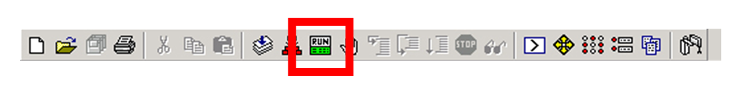
\includegraphics[width=\textwidth]{/Eps/13_Zaganjanje_programov.eps}
    \vspace{-0.9cm}
    \caption{Zaganjanje napisanih programov}
    \label{fZaganjanjePrograma}
\end{figure}

    \item[5)] Napisan program zaženemo tako, da kliknemo ikono, prikazano na sliki \\ %
    \ref{fZaganjanjePrograma}, nato pa še gumb \textbf{Start main}.%

\end{enumerate}





\subsection{Vključitev pogonskih motorjev}

Ob zagonu programskega okolja Epson RC+ pogonski motorji nimajo
napajanja. Napajanje vključimo tako, da kliknemo na ikono, ki je
označena na sliki \ref{fOrodnaVrsticaKontrolno}, nato pa se odpre
okno s slike \ref{fOrodnaVrsticaKontrolnoOkno}.

\begin{figure}[h]
    \centering
    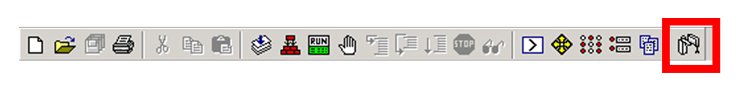
\includegraphics[width=\textwidth]{/Eps/05_Orodna_vrstica.eps}
    \vspace{-0.9cm}
    \caption{Orodna vrstica in ikona za odpiranje kontrolnega okna}
    \label{fOrodnaVrsticaKontrolno}
\end{figure}
\vspace{-0.3cm}
\begin{figure}[h]
    \centering
    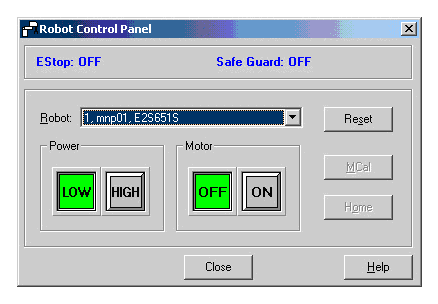
\includegraphics[width=0.9\textwidth]{/Eps/06_Kontrolno_okno.eps}
    \vspace{-0.3cm}
    \caption{Kontrolno okno robota}
    \label{fOrodnaVrsticaKontrolnoOkno}
\end{figure}


\noindent %
\textbf{\underline{Izbire oziroma gumbi  v kontrolnem oknu}} %
\\
\begin{enumerate}
    \item[-] \textbf{EStop: (OFF/ON)} \\%
        \hspace*{1.0cm}    $\longrightarrow$ Napis signalizira, ali je pritisnjena tipka \textbf{(črna škatla na mizi s \\%
        \hspace*{1.7cm}    kovinskim gumbom v sredini)} zasilnega izklopa. %
    \item[-] \textbf{Safe Guard: (OFF/ON)} \\%
        \hspace*{1.0cm}    $\longrightarrow$ Napis signalizira, ali je nekdo vstopil v varnostno kletko robota. %
    \item[-] izbira \textbf{Robot:} $\longrightarrow$ Izberemo robot (v našem primeru je samo eden). %
    \item[-] gumb \textbf{Reset} $\longrightarrow$ Resetiramo stanje po napaki ali pritisnjeni zasilni tipki. %
    \item[-] gumb \textbf{Help} $\longrightarrow$ S pritiskom prikličemo pomoč. %
    \item[-] gumb \textbf{Close} $\longrightarrow$ S pritiskom zapremo okno. %
\end{enumerate}

\noindent %
\textbf{Power}
\begin{enumerate}
    \item[-] \textbf{LOW} $\longrightarrow$ Pogonski motorji delujejo v načinu \textbf{nizke} moči. %
    \item[-] \textbf{HIGH} $\longrightarrow$ Pogonski motorji delujejo v načinu \textbf{visoke} moči. %
\end{enumerate}

\noindent %
\textbf{Motor}
\begin{enumerate}
    \item[-] \textbf{OFF} $\longrightarrow$ Izključimo napajanje pogonskih motorjev \emph{(v tem stanju lahko \\%
        \hspace*{1.5cm}    robot premikamo z roko)}. %
    \item[-] \textbf{ON} $\longrightarrow$ Vključimo napajanje pogonskih motorjev \emph{(robot lahko premikamo \\%
        \hspace*{1.3cm}    le preko uporabniškega vmesnika)}. %
\end{enumerate}



% ********************************************************************
\noindent %
\begin{mdframed}[backgroundcolor=red!80, shadow=true,roundcorner=8pt]
%\begin{tikzpicture}
%    \node [fill=red,rounded corners=5pt] {
%    \begin{minipage}{0.98\textwidth}
        \vspace{0.2cm}
        \large
\textcolor[rgb]{1.00,1.00,0.00}{\textbf{V fazi programiranja in testiranja mora biti zaradi vaše varnosti in morebitnih poškodb opreme}}\\ %
\textcolor[rgb]{1.00,1.00,0.00}{\LARGE \textbf{vedno vklopljena opcija Power LOW!}} \\ %
        \vspace{0.2cm}
\textcolor[rgb]{1.00,1.00,0.00}{\small Opcija Power High je namenjena doseganju polne dinamike robota v industrijskem okolju.} %
        \vspace{0.2cm}
%    \end{minipage}
%    };
%\end{tikzpicture}
\end{mdframed}
\normalsize
% ********************************************************************







\vspace{0.0cm}
\subsection{Upravljanje z digitalnimi vhodi in izhodi}

Krmilnik v osnovi omogoča spremljanje in upoštevanje 16 digitalnih
vhodnih signalov in 16 digitalnih izhodnih signalov. Za namen
izvajanja prijemanja pokrovčkov je na robot nameščeno pnevmatsko
prijemalo. Pnevmatski cilinder prijemala krmilimo z monostabilnim
elektropnevmatskim ventilom, ki ga krmilimo z enim digitalnim
izhodom iz robotskega krmilnika. Po pritisku na ikono s slike
\ref{fOrodnaVrsticaIO} se odpre okno s slike
\ref{fOrodnaVrsticaIOOkno}.

\begin{figure}[h]
    \centering
    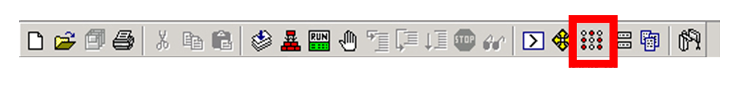
\includegraphics[width=0.99\textwidth]{/Eps/07_Orodna_vrstica_IO.eps}
    \vspace{-0.9cm}
    \caption{Orodna vrstica in ikona za odprtje okna upravljanja z digitalnimi vhodi in izhodi}
    \label{fOrodnaVrsticaIO}
\end{figure}

\begin{figure}[h]
    \centering
    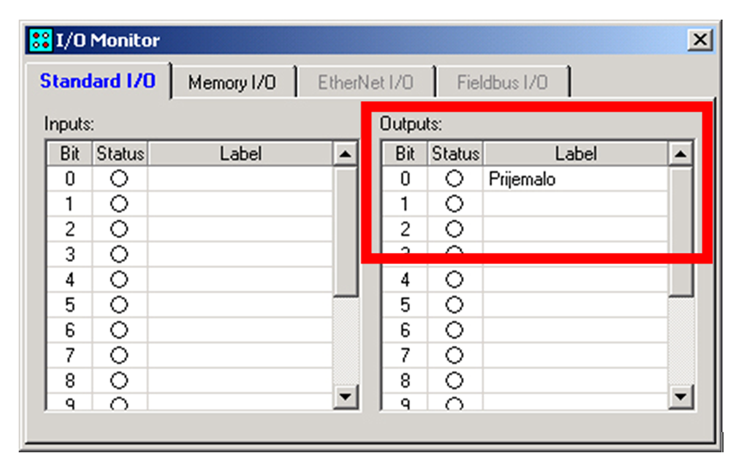
\includegraphics[width=0.85\textwidth]{/Eps/08_IO.eps}
    \vspace{-0.3cm}
    \caption{Okno za upravljanje z digitalnimi vhodi in izhodi}
    \label{fOrodnaVrsticaIOOkno}
\end{figure}


\noindent %
\textbf{\underline{Okno za upravljanje z digitalnimi vhodi in izhodi}} %
\\
\begin{enumerate}
    \item[-] \textbf{Standard I/O} $\longrightarrow$ Zavihek, kjer upravljamo z digitalnimi vhodi in izhodi. %
    \item[-] \textbf{Inputs} $\longrightarrow$ Digitalni vhodi \emph{(biti od 0 do 15)}. %
    \item[-] \textbf{Outputs} $\longrightarrow$ Digitalni izhodi \emph{(biti od 0 do 15)}. %
    \item[-] \textbf{Memory I/O} $\longrightarrow$ Zavihek za upravljanje z biti spomina (512 bitov), upo-\\%
        \hspace*{2.7cm}    rabljeni za komunikacijo med opravili (task) programa. %
\end{enumerate}


Prijemalo oziroma njegov elektropnevmatski ventil je priklopljen
na \textbf{digitalni izhod številka 0}. \textbf{Ta signal vklopimo
oziroma izklopimo z dvakratnim klikom na krogec v stolpcu Status}
(Slika \ref{fOrodnaVrsticaIOOkno}). Prijemalo je odprto, ko je
krogec prazen, in zaprto ob polnem krogcu.








\vspace{0.2cm}
\subsection{Okno za premikanje robota in učenje točk}

Robot premikamo na različne načine, spremljamo trenutno lego in
shranjujemo lego vrha robota v oknu, katerega odpremo s pritiskom na
gumb s slike \ref{fOrodnaVrsticaPremikanje}.
%okna s slike \ref{fOrodnaVrsticaPremikanjeOkno}. Okno odpremo s
\vspace{0.2cm} %
\begin{figure}[h]
    \centering
    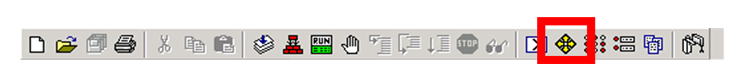
\includegraphics[width=\textwidth]{/Eps/09_Orodna_vrstica_Premikanje.eps}
    \vspace{-0.9cm}
    \caption{Orodna vrstica in ikona za okno za premikanje robota in učenje točk}
    \label{fOrodnaVrsticaPremikanje}
\end{figure}

\noindent %
\textbf{\underline{Ukazi za premikanje robota}} %
\vspace{0.5cm}
\begin{enumerate}

    \item[-] \textbf{Jog Mode} $\longrightarrow$ Izbiramo koordinatni sistem za premikanje robota (\emph{World,\\ %
        \hspace*{2.3cm}         Tool, Joint}). %
\vspace{0.2cm}
    \item[-] \textbf{Jog Distance} $\longrightarrow$ Izberemo korak premika, kjer prednastavljene korake \\%
        \hspace*{2.8cm}            izberemo s pritiskom na ustrezen krogec (Long, Medium\\%
        \hspace*{2.8cm}            ali Short). V poljih lahko vrednosti tudi spreminjamo. %
\vspace{0.2cm}
    \item[-] \textbf{Current Position} \\ %
        \hspace*{1.0cm}    $\longrightarrow$ Izpisuje se trenutna lega izbranega orodja (npr. \emph{Tool 0}) v refe-\\%
        \hspace*{1.7cm}    renčnem koordinatnem sistemu (izbira \textbf{World}). \\%
        \hspace*{1.0cm}    $\longrightarrow$ Izpisujejo se trenutni koti v sklepih v stopinjah (izbira \textbf{Joint}).\\%
        \hspace*{1.0cm}    $\longrightarrow$ Izpisujejo se trenutni pulzi enkoderjev v sklepih (izbira \textbf{Pulse}).\\%
\vspace{0.2cm}
    \item[-] \textbf{Jogging $\&$ Motion Commands} \\ %
        \hspace*{1.0cm}    $\longrightarrow$ S puščicami vodimo robot v izbrani smeri koordinatnega si-\\%
        \hspace*{1.7cm}    stema (\emph{Jog Mode = World ali Tool}) ali ga rotiramo po sklepih \\%
        \hspace*{1.7cm}  (\emph{Jog Mode = Joint}). %
\end{enumerate}

%\begin{figure}[h]
%    \centering
%    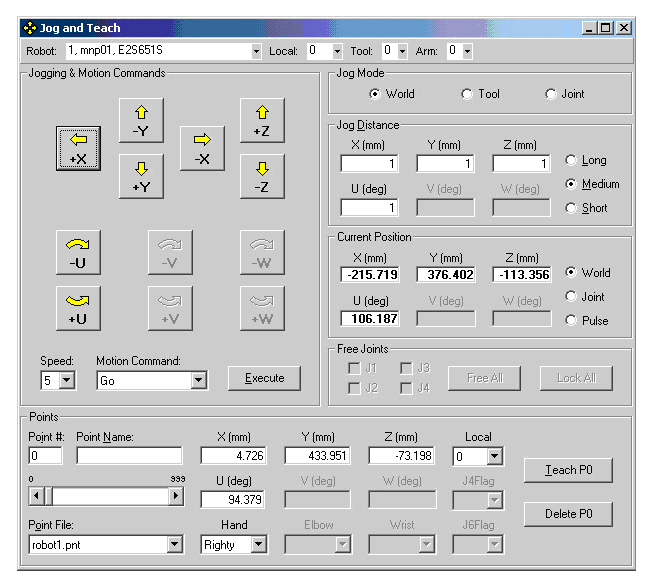
\includegraphics[width=0.97\textwidth]{Poglavja_Slike/02_SCARA_Umetni_vid/Slike/Eps/10_Premikanje.eps}
%    \vspace{-0.3cm}
%    \caption{Okno za premikanje robota in učenje točk}
%    \label{fOrodnaVrsticaPremikanjeOkno}
%\end{figure}

\begin{figure}[h]
    \centering
    \includegraphics[width=0.97\textwidth]{/Eps/11_Ukazi_za_premikanje.eps}
    \vspace{-0.3cm}
    \caption{Ukazi za premikanje robota}
    \label{fUkaziPremikanjeRobota}
\end{figure}

\noindent %
\textbf{\underline{Ukazi za učenje točk}} %

\begin{enumerate}

    \item[-] \textbf{Points} $\longrightarrow$ Razdelek omogoča shranjevanje trenutnih leg vrha robota v da- \\ %
        \hspace*{1.75cm}      toteko (\emph{Point File}); največje število točk v eni datoteki je 1000.\\ %
        \hspace*{1.75cm}      V okno Point $\#$: ročno vpišemo številko točke ali pa jo nasta- \\ %
        \hspace*{1.75cm}      vimo z drsnikom spodaj. Trenutne vrednosti lege  X, Y, Z, U \\ %
        \hspace*{1.75cm}       in Local lahko poljubno spreminjamo. \textbf{Točko shranimo} s pri- \\ %
        \hspace*{1.75cm}      tiskom na \textbf{gumb Teach P$\#$, zbrišemo} pa jo z \textbf{Delete P$\#$}. \\%

\end{enumerate}

\begin{figure}[h]
    \centering
    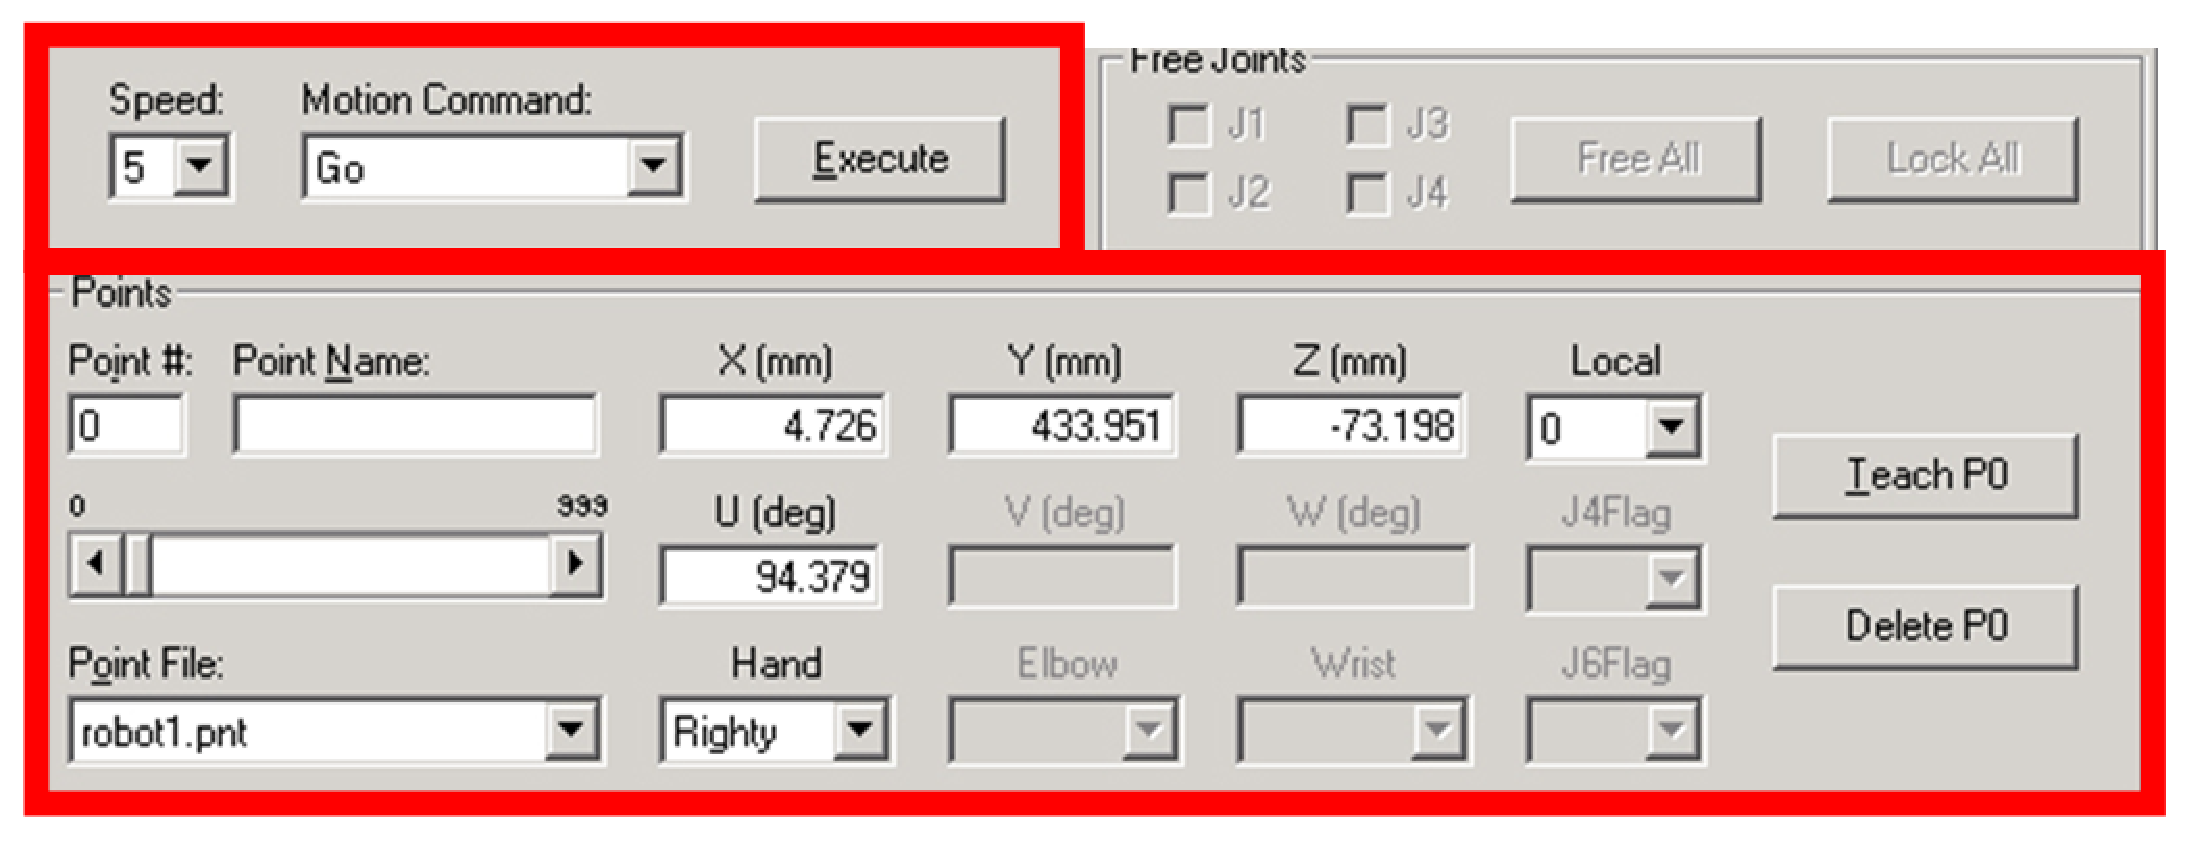
\includegraphics[width=0.9\textwidth]{/Eps/12_Ucenje_tock.eps}
    \vspace{-0.3cm}
    \caption{Ukazi za učenje točk}
    \label{fUkaziUcenjeTock}
\end{figure}


Robot lahko v shranjene lege premikamo z izbirami na sliki
\ref{fUkaziUcenjeTock}, skrajno levo zgoraj. Hitrost premika
nastavimo z izbiro \emph{Speed}, način giba z izbiro \emph{Motion
Command}, gibanje pa štartamo z gumbom \textbf{Execute}.


\vspace{0.0cm} %
\section{1. del naloge}

V 1. delu naloge spoznate ukaze in postopek za prijem zamaška,
privitje zamaška na ustje plastenke, njegovo odvitje z ustja ter
spust zamaška na začetno lego. Ta postopek je namreč večji del
programa, ki je v 2. delu naloge že napisan in ga le zaženete.

\subsection{Ukazi, potrebni za izvedbo naloge}
\vspace{0.3cm}

\begin{mdframed}[backgroundcolor=green!20, shadow=true,roundcorner=8pt]
%\begin{tikzpicture}
%    \node [fill=green,rounded corners=5pt] {
%    \begin{minipage}{0.98\textwidth}
        \vspace{0.2cm}
\textbf{Jump} $\longrightarrow$ premik vrha robota iz točke v točko (recimo iz P0 v P1), ki ga \\
\hspace*{1.6cm}  razdelimo na: \vspace*{0.3cm} \\ %
\hspace*{1.6cm} 1) translacija navzgor z nespremenjeno orientacijo; \\ %
\hspace*{1.6cm} 2) sinhrono premikanje sklepov, pri čemer se orientacija vrha \\ %
\hspace*{2.05cm} robota spremeni, če je drugačna v ciljni točki; \\ %
\hspace*{1.6cm} 3) translacija navzdol v ciljno lego z ustrezno orientacijo vrha \\%
\hspace*{2.05cm} robota. %
        \vspace{0.2cm}
%    \end{minipage}
%    };
%\end{tikzpicture}
\end{mdframed}

\begin{figure}[h]
    \center
    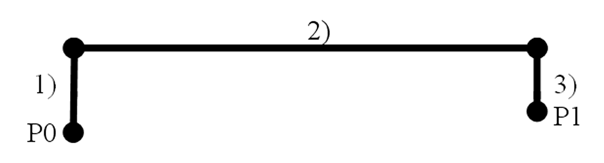
\includegraphics[width=0.65\textwidth]{/Eps/14_Jump.eps}
    \vspace{-0.3cm}
    \caption{Premikanje vrha robota pri uporabi ukaza Jump}
    \label{fJump}
\end{figure}

\begin{mdframed}[backgroundcolor=green!20, shadow=true,roundcorner=8pt]
%\begin{tikzpicture}
%    \node [fill=green,rounded corners=5pt] {
%    \begin{minipage}{0.98\textwidth}
        \vspace{0.2cm}
\textbf{Go} $\longrightarrow$ premik vrha robota iz točke v točko (P0 v P1) s sinhronim premika- \\ %
\hspace*{1.2cm} njem sklepov. Sinhrono  premikanje pomeni, da se vsi sklepi, katerih \\ %
\hspace*{1.2cm} premik je potreben, začnejo premikati hkrati in tudi hkrati končajo. \vspace*{0.3cm}\\ %
\hspace*{1.2cm} \emph{Primer: Za dosego končne lege se mora prvi segment  zarotirati za} \\ %
\hspace*{1.2cm} \emph{213$^\circ$, tretji pa translirati za 8 mm. Rotacijo prvega sklepa robot} \\ %
\hspace*{1.2cm} \emph{opravlja z nastavljeno hitrostjo v programu (največji premik), hitrost} \\ %
\hspace*{1.2cm} \emph{translacije pa prilagodi času, ki je potreben za izvršitev rotacije} \\ %
\hspace*{1.2cm} \emph{prvega sklepa.}  %
        \vspace{0.2cm}
%    \end{minipage}
%    };
%\end{tikzpicture}
\end{mdframed}

\begin{figure}[h]
    \center
    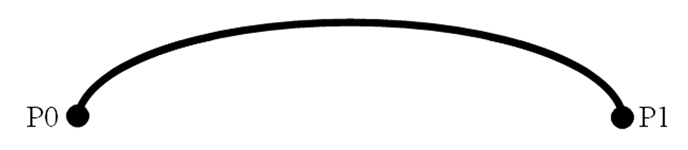
\includegraphics[width=0.65\textwidth]{/Eps/15_Go.eps}
    \vspace{-0.3cm}
    \caption{Premikanje vrha robota, ko je uporabljen ukaz Go}
    \label{fJump}
\end{figure}

\textbf{Motor P} $\longrightarrow$ Parameter (P) \textbf{On} vključi napajanje motorjev, parameter \\ %
\hspace*{2.1cm} \textbf{Off} pa napajanje izključi (\emph{primer: Motor On}). \vspace{-0.3cm} \\ %

\textbf{Power P} $\longrightarrow$ Nastavitev moči delovanja motorjev. Parameter (P) \textbf{Low} \\ %
\hspace*{2.1cm} nastavi nizek režim, parameter \textbf{High} pa večji režim moči.  \vspace{-0.3cm} \\ %

\textbf{Speed N} $\longrightarrow$ Največja hitrost (N) gibanja v odstotkih (od 1 $\%$ do 100 $\%$) glede \\ %
\hspace*{2.1cm}   na maksimum (\emph{primer: Speed 40}). \vspace{-0.3cm} \\ %

\textbf{Accel N,M} $\longrightarrow$ Največji pospešek (N) in pojemek (M) v odstotkih (od 1 $\%$ do\\ %
\hspace*{2.4cm} 100 $\%$) glede na maksimum (\emph{primer: Accel 30, 10}). \vspace{-0.3cm} \\ %

\textbf{On N} $\longrightarrow$ Dvig digitalnega signala na naslovu N (\emph{primer: On 0}). \vspace{-0.3cm} \\ %

\textbf{Off N} $\longrightarrow$ Spust digitalnega signala na naslovu N (\emph{primer Off 0}). \vspace{-0.3cm} \\ %

\textbf{Wait N} $\longrightarrow$ Ustavitev izvajanja programa za N sekund (\emph{primer: Wait 1.3}). \vspace{-0.3cm} \\ %


\subsection{Koraki za izvedbo naloge}
\vspace{0.3cm}

\begin{mdframed}[backgroundcolor=green!20, shadow=true,roundcorner=8pt]
%\begin{tikzpicture}
%    \node [fill=green,rounded corners=5pt] {
%    \begin{minipage}{0.98\textwidth}
        \vspace{0.2cm}
\noindent %
\textbf{Napišite program (primer spodaj) za premik robota iz točke P0 v P1, prijem zamaška in njegov prenos nad ustje plastenke v točki P2. Sledi privijanje v točko P3. Po krajši pavzi vrstni red nalog obrnite in odložite zamašek na izhodiščno pozicijo, robot pa naj se vrne v izhodiščno točko P0. Vsaka operacija prijemanja in spuščanja zamaška zahteva kratke premore, zato uporabite ukaz Wait.} \\ %
\\
\\
\small
\texttt{Function main} \\%
    \hspace*{0.3cm}   \texttt{Motor On        \small\hspace{0.75cm} ' Vključitev napajanja motorjev.} \\%
    \hspace*{0.3cm}   \texttt{Power Low       \small\hspace{0.55cm} ' Nizka moč delovanja motorjev.} \\%
    \hspace*{0.3cm}   \texttt{Speed 20        \small\hspace{0.75cm} ' Hitrost gibanja na 20$\%$ največje.} \\%
    \hspace*{0.3cm}   \texttt{Accel 20, 20    \small\hspace{0.00cm} ' Pospešek in pojemek na 20$\%$ največjega.} \\%
    \hspace*{0.3cm}   \texttt{Off 0           \small\hspace{1.35cm} ' Preventivno odprtje prijemala.} \\%
    \hspace*{0.3cm}   \texttt{Wait 0.2        \small\hspace{0.80cm} ' Pavza 0.2 sekunde.} \\%
     \\%
    \hspace*{0.3cm}   \texttt{Go P0           \small\hspace{1.40cm} ' Premik robota v točko P0.} \\%
    \hspace*{0.3cm}   \texttt{Jump P1         \small\hspace{1.00cm} ' Premik robota v točko P1.} \\%
    \hspace*{0.3cm}   . \\%
    \hspace*{0.3cm}   . \\%
    \hspace*{0.3cm}   . \\%
\texttt{Fend} \\%
\normalsize

%    \end{minipage}
%    };
%\end{tikzpicture}
\end{mdframed}

\begin{mdframed}[backgroundcolor=blue!20, shadow=true,roundcorner=8pt]
%\begin{tikzpicture}
%    \node [fill=blue,rounded corners=5pt] {
%    \begin{minipage}{0.98\textwidth}
        \vspace{0.2cm}
\hspace*{0.05cm} 1) Ustvarite nov projekt (Projects$\setminus$StudentskeVaje) in vpišite njegovo ime v \\ %
\hspace*{0.50cm} polje, ki ga razvojno okolje ponudi. \vspace*{0.3cm} \\ %
\hspace*{0.05cm} 2) V oknu za programiranje zapišete \texttt{Function main} in dve vrstici \\ %
\hspace*{0.5cm} nižje še \texttt{Fend}.  \vspace*{0.3cm} \\ %
\hspace*{0.05cm} 3) Robot ne sme imeti vključenega napajanja motorjev (Slika \ref{fOrodnaVrsticaKontrolnoOkno}). \vspace*{0.3cm} \\ %
\hspace*{0.05cm} 4) Odprite okno Jog and Teach s klikom na ustrezno ikono (Slika \ref{fOrodnaVrsticaPremikanje}). \vspace*{0.3cm} \\ %
\hspace*{0.05cm} 5) Odprite okno I/O Monitor (Slika \ref{fOrodnaVrsticaIOOkno}) in preverite, če je prijemalo odprto \\ %
\hspace*{0.5cm} (izhodni naslov 0 ne sme biti izbran). \vspace*{0.3cm} \\ %
\hspace*{0.05cm} 6) Na mizo v delovnem prostoru robota postavite zamašek. \vspace*{0.3cm} \\ %
\hspace*{0.05cm} 7) Robot ročno postavite v poljubno lego v delovnem prostoru robota. \vspace*{0.3cm} \\ %
\hspace*{0.05cm} 8) V oknu Jog and Teach (Slika \ref{fUkaziUcenjeTock}) shranite lego robota kot točko P0. \vspace*{0.3cm} \\ %
\hspace*{0.05cm} 9) Robot z roko postavite tako, da lahko prime zamašek (lega, ki ji sledi \\ %
\hspace*{0.5cm} stisk prijemala). Za vertikalni premik tretjega segmenta sprostite zavoro \\ %
\hspace*{0.5cm} s pritiskom na bel gumb (Slika \ref{fKontrolna_plosca}). \vspace*{0.3cm} \\ %
10) V oknu Jog and Teach (Slika \ref{fUkaziUcenjeTock}) shranite lego robota kot točko P1. \vspace*{0.3cm} \\ %
11) V oknu I/O Monitor (Slika \ref{fOrodnaVrsticaIOOkno}) kliknite na naslov izhodnega digitalnega \\ %
\hspace*{0.55cm} signala 0 za stisk prijemala. \vspace*{0.3cm} \\ %
12) Robot s prijetim zamaškom z roko premaknite tik nad ustje plastenke. \\ %
\hspace*{0.55cm} Za vertikalni premik tretjega segmenta sprostite zavoro s pritiskom na \\ %
\hspace*{0.55cm} bel gumb (Slika \ref{fKontrolna_plosca}). \vspace*{0.3cm} \\ %
13) V oknu Jog and Teach (Slika \ref{fUkaziUcenjeTock}) shranite lego robota kot točko P2.  \vspace*{0.3cm} \\ %
14) Zadnjo os robota s prijetim zamaškom z roko rotirajte (vrtite) in \\ %
\hspace*{0.55cm} vertikalno translirajte (pomik navzdol), da privijete zamašek.  Za \\ %
\hspace*{0.55cm} vertikalni premik tretjega segmenta sprostite zavoro s pritiskom na \\ %
\hspace*{0.55cm} bel gumb (Slika \ref{fKontrolna_plosca}). \vspace*{0.3cm} \\ %
15) V oknu Jog and Teach (Slika \ref{fUkaziUcenjeTock}) shranite lego robota kot točko P3. \vspace*{0.3cm} \\ %
16) V oknu I/O Monitor (Slika \ref{fOrodnaVrsticaIOOkno}) kliknite na naslov izhodnega digitalnega \\ %
\hspace*{0.55cm} signala 0 za spust zamaška. \vspace*{0.3cm} \\ %
17) Robot z roko umaknite iznad ustja plastenke. %
%    \end{minipage}
%    };
%\end{tikzpicture}
\end{mdframed}



\newpage
\section{Matlab in umetni vid}
\vspace{0.3cm}

Programsko okolje Matlab s svojo široko paleto funkcij in orodij
omogoča tudi učinkovito delo z umetnim vidom oziroma obdelavo slik
ter vzorcev. Pri vaji sta pomembni predvsem naslednji orodji:
\vspace*{0.2cm} %
\begin{enumerate}
\item[1)] \textbf{Image Acquisition Toolbox} $\longrightarrow$ skrbi za zajem slike in videa ter strojno \\%
\hspace*{5.1cm} podporo. \\ %
\vspace*{-0.37cm} %
\item[2)] \textbf{Image Processing Toolbox}  $\longrightarrow$ obdelava slike, razpoznavanje vzorcev,\\%
\hspace*{5.0cm} transformacije, ugotavljanje najrazlič-\\%
\hspace*{5.0cm} nejših lastnosti slik itd. \\ %
\end{enumerate}

Matlab je v osnovi namenjen za numerično računanje, še posebej
manipulaciji matričnih funkcij. Sliko lahko predstavimo kot
matriko. Sivinska je zapisana kot M$\times$N matrika (Slika
\ref{fMatrikaA}), barvna pa kot kot M$\times$N$\times$3 matrika,
kjer tretja dimenzija predstavlja posamezno RGB komponento (Slika
\ref{fMatrikaB}).

\begin{figure}[h]
  \begin{center}
    \subfigure[Matrika sivinske slike dimenzije M$\times$N]
    {
        \label{fMatrikaA}
        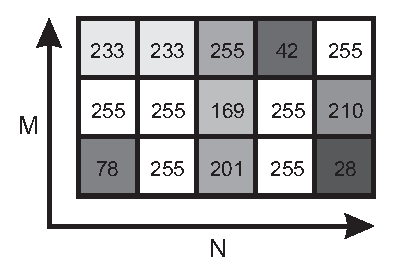
\includegraphics[scale=0.8]{/Eps/16_Sivinjska_slika.eps}
    }
    \subfigure[Matrika barvne slike dimenzije M$\times$N$\times$3]
    {
        \label{fMatrikaB}
        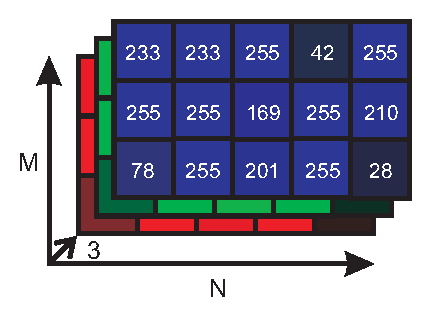
\includegraphics[scale=0.8]{/Eps/17_Barvna_slika.eps}
    } \\
  \end{center}
  \vspace{-0.5cm}
  \caption{Primera matrik sivinske in barvne slike}
  \label{fMatrike}
\end{figure}


\vspace{0.0cm}
\subsection{Video sistem}
\vspace{0.3cm}


\begin{figure}[h]
    \center
    \includegraphics[width=0.7\textwidth]{/Eps/18_Kamera.eps}
    \vspace{-0.3cm}
    \caption{Video sistem nad mizo robota}
    \label{fKamera}
\end{figure}

\noindent%
Karakteristike video sistema s slike \ref{fKamera} so:

\begin{itemize}
    \item \vspace*{-0.1cm} kamera The Imaging source DMK 21AF04 s Firewire vodilom, %
    \item \vspace*{-0.1cm} slikovni senzor CCD velikosti 640$\times$480 slikovnih elementov, %
    \item \vspace*{-0.1cm} 256 sivinskih odtenkov, %
    \item \vspace*{-0.1cm} digitalen zajem in prenos slike, %
    \item \vspace*{-0.1cm} objektiv z 8 mm goriščne razdalje. %
\end{itemize}



\subsection{2. del naloge }

\begin{mdframed}[backgroundcolor=green!20, shadow=true,roundcorner=8pt]
%\begin{tikzpicture}
%    \node [fill=green,rounded corners=5pt] {
%    \begin{minipage}{0.98\textwidth}
        \vspace{0.2cm}
Na sliki \ref{fPostavitevKS} so predstavljeni vsi nastopajoči
koordinatni sistemi. Najosnovnejši je \textbf{referenčni koordinatni
sistem robota}, ki leži v prvem sklepu robota Epson. V verigi robota
nastopa še \textbf{koordinatni sistem vrha robota}, ki je pripet na
zadnji sklep robota. Ker v sistem hočemo vključiti še informacije
dobljene s slike video kamere, v ogljišče njenega vidnega polja
pripnemo \textbf{koordinatni sistem kamere}. V vidnem polju kamere
bodo postavljeni objekti, ki imajo svojo lego (pozicijo in
orientacijo). Zato zaradi splošnosti tudi objektu v vidnem polju
kamere pripnemo \textbf{ koordinatni sistem objekta}.
%    \end{minipage}
%    };
%\end{tikzpicture}
\end{mdframed}

\begin{figure}[h]
    \center
    \includegraphics[width=0.65\textwidth]{/Eps/19_Koordinatni_sistemi.eps}
    \vspace{-0.3cm}
    \caption{Postavitev koordinatnih sistemov}
    \label{fPostavitevKS}
\end{figure}



\begin{figure}[t]
    \center
    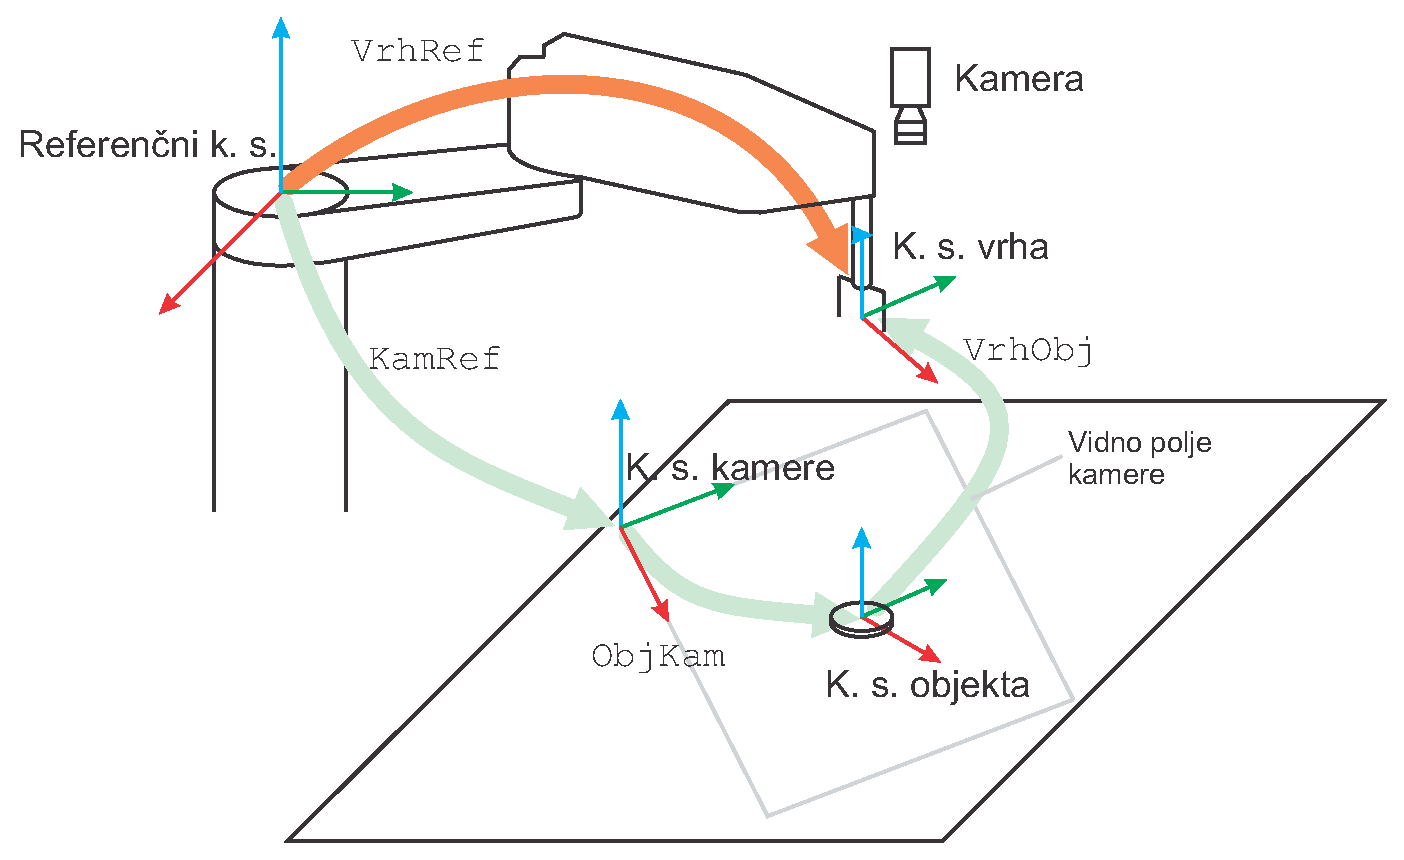
\includegraphics[width=0.8\textwidth]{/Eps/20_Transformacije_slo.eps}
    \vspace{-0.3cm}
    \caption{Transformacije med koordinatnimi sistemi}
    \label{fTransformacija}
\end{figure}

\vspace*{-0.5cm} %

\begin{mdframed}[backgroundcolor=green!20, shadow=true,roundcorner=8pt]
%\begin{tikzpicture}
%    \node [fill=green,rounded corners=5pt] {
%    \begin{minipage}{0.98\textwidth}
        \vspace{0.2cm}
Na sliki \ref{fTransformacija} so prikazane transformacije med
omenjenimi koordinatnimi sistemi. Najbolj očitna je transformacija,
ki ponazarja \textbf{lego koordinatnega sistema vrha v referenčnem
koordinatnem sistemu robota} in je odvisna od spremenljivk (koti in
pozicije) v sklepih robota.
\\
\\
Lego vrha robota lahko izrazimo oz. izračunamo tudi drugače, vendar
je potrebno poznati naslednje homogene transformacijske matrike:
\vspace*{-0.2cm} %
\begin{itemize}
    \item[-] lego koordinatnega sistema kamere v referenčnem koordinatnem sistemu robota (KamRef),\vspace*{-0.7cm} \\ %
    \item[-] lego koordinatnega sistema objekta v koordinatnem sistemu video kamere (ObjKam)\vspace*{-0.7cm}\\ %
    \item[-] lego vrha robota v koordinatnem sistemu objekta (VrhObj).\\%
\end{itemize}
\vspace*{-0.2cm} %
Omenjeno enakost zapišemo v obliki matrične
enačbe:

\begin{center}
\textbf{VrhRef = KamRef $\bullet$ ObjKam $\bullet$ VrhObj}\\ %
\end{center}
\vspace*{-0.3cm}
%\end{minipage}
%    };
%\end{tikzpicture}

\end{mdframed}

\vspace*{0.3cm}%
Razlaga okrajšav uporabljenih koordinatnih sistemov:
\vspace*{-0.2cm}%
\begin{itemize}
    \item[] \vspace*{-0.1cm} \textbf{VrhRef} $\longrightarrow$ Lega vrha robota v referenčnem koordinatnem sistemu.\\%
    \hspace*{2.0cm} \emph{Lego odčitamo v okolju Epson RC+ (okno na sliki \ref{fUkaziUcenjeTock})}. %
    \item[] \vspace*{-0.2cm} \textbf{KamRef} $\longrightarrow$ Lega koordinatnega sistema kamere v referenčnem \\ %
    \hspace*{2.15cm} koordinatnem sistemu robota.\\
    \item[] \vspace*{-0.7cm} \textbf{ObjKam} $\longrightarrow$ Lega koordinatnega sistema objekta v koordinatnem \\ %
    \hspace*{2.2cm} sistemu robota.\\
    \item[] \vspace*{-0.7cm} \textbf{VrhObj} $\longrightarrow$ Lega koordinatnega sistema vrha robota (prijemala) v \\ %
    \hspace*{2.2cm} koordinatnem sistemu objekta.\\
\end{itemize}



\begin{figure}[t]
    \center
    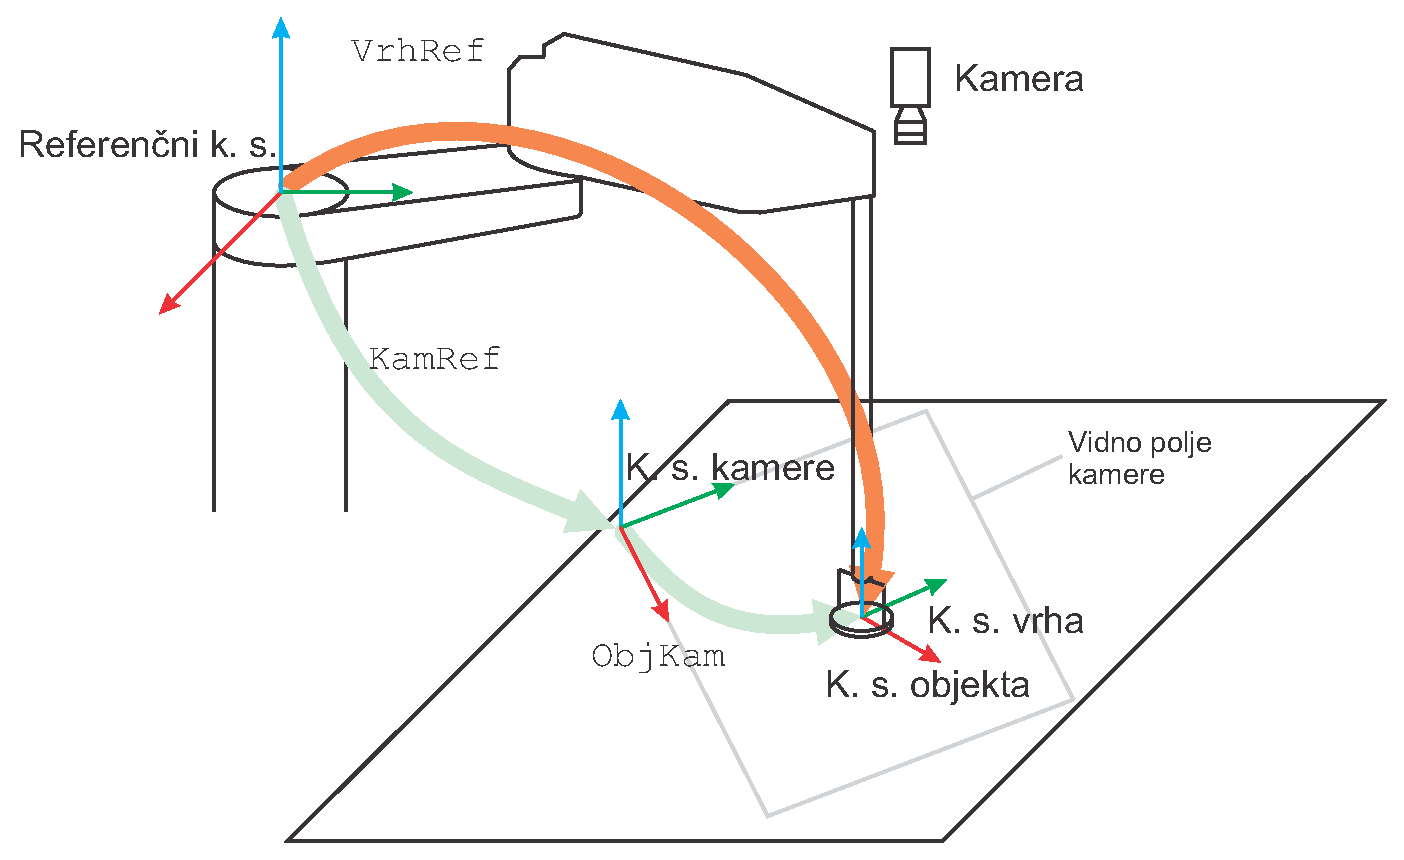
\includegraphics[width=0.8\textwidth]{/Eps/20_Transformacije_prijem_slo.eps}
    \vspace{-0.3cm}
    \caption{Transformacije med koordinatnimi sistemi pri prijemu objekta}
    \label{fTransformacijaPrijem}
\end{figure}

\noindent %
\begin{mdframed}[backgroundcolor=green!20, shadow=true,roundcorner=8pt]
%\begin{tikzpicture}
%    \node [fill=green,rounded corners=5pt] {
%    \begin{minipage}{0.98\textwidth}
        \vspace{0.2cm}
Ko robot prime objekt, želimo poravnavo koordinatnega sistema vrha
in koordinatnega sistema objekta. V tem primeru transformacija
VrhObj izgine oz. matematično gledano matrika postane enotska
matrika (po diagonali 1).
\\
\\
V tem primeru se enačba s prejšnje strani malenkostno poenostavi:

\begin{equation}
\centering
\textbf{VrhRef = KamRef $\bullet$ ObjKam $\bullet$ I} %
\label{eEqSimple}
\end{equation}

Enačba \ref{eEqSimple} opisuje lego koordinatnega sistema vrha
robota v referenčnem koordinatnem sistemu (VrhRef) ob prijemu
objekta. Uporabna je v primeru, če poznamo lego koordinatnega
sistema objekta v koordinatnem sistemu kamere (ObjKam) in lego
koordinatnega sistema kamere v referenčnem koordinatnem sistemu
robota (KamRef). Tako lahko izračunamo lego koordinatnega sistema
objekta v referenčnem koordinatnem sistemu robota in v to lego lahko
pošljemo vrh robota (VrhRef).
\\
\\
\textbf{če hočemo robot premakniti v neko lego (VrhRef) v vidnem
polju kamere in tako prijeti objekt (VrhObj = I), je potrebno
poznati obe transformaciji na desni strani enačbe (KamRef in
ObjKam). Vendar pa ob pričetku izvajanja naloge ni poznana ne ena ne
druga lega.}
\\
\\
V nadaljevanju bomo pokazali, da je določitev \textbf{ObjKam }iz
slike preprosto opravilo. Enako velja za določitev \textbf{VrhRef}.
Na podlagi teh dveh določitev lahko iz enačbe \ref{eEqSimple}
izrazimo kot neznanko \textbf{KamRef} in jo tako izračunamo. Šele
nato lahko zgornjo enačbo uporabljamo za izračun \textbf{VrhRef}, ki
premakne robot v lego za prijem objekta, katerega lego smo določili
iz slike kamere.
%\end{minipage}
%    };
%\end{tikzpicture}
\end{mdframed}

\noindent %
\textbf{\underline{Določitev matrike ObjKam}} %
%\textbf{\underline{Določitev T_obj2cam}} %
\\
~\\
Za določitev lege koordinatnega sistema objekta v koordinatnem
sistemu kamere (\textbf{ObjKam}) uporabimo plastično ploščo s tremi
črnimi pikami (Slika \ref{fKalibracijskiList}). Ena pika predstavlja
koordinatno izhodišče O, ostali dve pa ležita na \emph{x} in
\emph{y} osi koordinatnega sistema objekta.

\vspace{0.1cm}
\begin{mdframed}[backgroundcolor=red!80, shadow=true,roundcorner=8pt]
%\begin{tikzpicture}
%    \node [fill=red,rounded corners=5pt] {
%    \begin{minipage}{0.93\textwidth}
        \vspace{0.1cm}
        \center
        \large
\textcolor[rgb]{1.00,1.00,0.00}{\LARGE\textbf{POKLIčI ASISTENTA!}}\\ %
\textcolor[rgb]{1.00,1.00,0.00}{\large Asistent naj na mizico pritrdi plastično ploščo za kalibracijo.} \\ %
%    \end{minipage}
%    };
%\end{tikzpicture}
\end{mdframed}
\vspace{0.1cm}

\begin{figure}[h]
    \center
    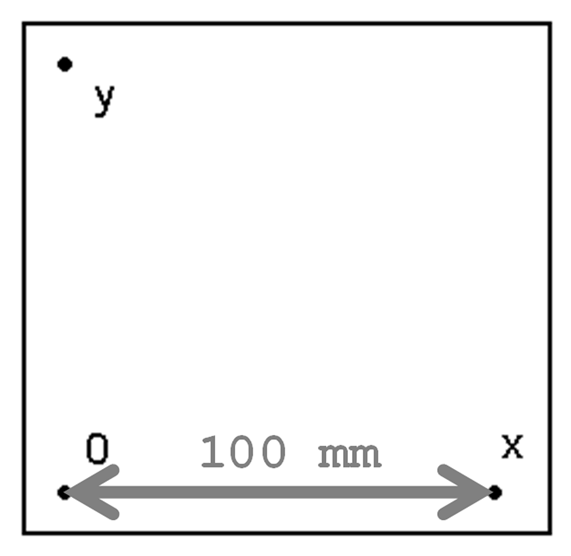
\includegraphics[width=0.6\textwidth]{/Eps/21_Kalibracijski_list}
    \vspace{-0.3cm}
    \caption{Kalibracijska plošča s točkami, ki predstavljajo k.s. objekta.}
    \label{fKalibracijskiList}
\end{figure}


\noindent %
\begin{mdframed}[backgroundcolor=blue!20, shadow=true,roundcorner=8pt]
%\begin{tikzpicture}
%    \node [fill=blue,rounded corners=5pt] {
%    \begin{minipage}{0.98\textwidth}
        \vspace{0.2cm}
        \textbf{List predstavlja objekt s koordinatnim sistemom in izhodiščem  v točki
        \emph{O}.}\\\\
        \textbf{Razdalja med točkami \emph{O} in \emph{X} ter \emph{O} in
        \emph{Y} znaša 100 mm in jo uporabimo za pretvorbo števila slikovnih elementov v milimetre.}
        \vspace{0.2cm}
%    \end{minipage}
%    };
%\end{tikzpicture}

\end{mdframed}
\normalsize

\noindent %
\textbf{Postopek za določitev matrike ObjKam} %
\\
Postopek za določanje matrike \textbf{ObjKam} je opisan v spodnjih
točkah. Pri delu uporabite programsko okolje Matlab.

\begin{enumerate}
\item[1)]  V okolju Matlab je potrebno izbrati delovno mapo
\textbf{C:$\setminus$Epson SCARA$\setminus$OR$\setminus$Epson$\_$kamera$\setminus$} in v  %
ukazni vrstici naložiti kalibracijo kamere. To storite z ukazom: \\ %
\vspace{-0.1cm}\\%
\textbf{$\gg$ load($\bm{'}$cameraParams.mat$\bm{'}$)} \verb"Enter" \\ %\Enter
\vspace{-0.2cm}\\%
%Toolbox je namenjen ugotavljanju parametrov kamere oz. uporabljenega
%objektiva (uporaba kalibracijskih vzorcev). Po potrditvi ukaza
%\emph{calib$\_$gui} se odpre okno, kjer kliknete gumb \emph{Standard
%(all the images are stored in memory)}. Postopek je že opravljen,
%zato kliknete gumb \emph{Load} in s tem naložite rezultate zadnje
%kalibracije. Trenutno prikazano okno zaprete s klikom na gumb
%\emph{Exit}.
V datoteki \textit{cameraParams.mat} so shranjene informacije o kameri in uporabljenem objektivu.
\vspace*{0.4cm} %

\item[2)] V naslednjem koraku je potrebno zajeti sliko s kamere in z ravnokar naloženimi %
parametri odstraniti popačenje objektiva. To storite tako, da v ukazno vrstico okolja %
Matlab vpišete: \\ %
\vspace{-0.3cm}\\%
\textbf{$\gg$ snapcalib2} \verb"Enter" \\ %\Enter
\vspace{-0.1cm}\\%
če je kamera pravilno priključena, se na zaslonu izpišejo parametri
kamere, kmalu zatem pa se pojavi okno z živo sliko.
\textbf{Postavite kalibracijsko ploščo v vidno polje kamere, da so na
sliki vidne vse tri točke. Sliko zajamete s pritiskom na tipko}
\verb"Enter". Slika se shrani kot calib$\_$image.tif, opravi se %\Enter
transformacija odstranjevanja popačenje objektiva in popravljena
slika se shrani kot calib$\_$image$\_$rect.tif.
\vspace*{0.2cm} %

\item[3)] Na zajeti in upragovljeni bitni sliki je potrebno ročno pokazati, kje se  %
pike koordinatnega sistema objekta (\emph{O}, \emph{X}, \emph{Y})  nahajajo. V ukazni vrstici okolja %
Matlab izvršite ukaz: \\ %
\vspace{-0.3cm}\\%
\textbf{$\gg$ select$\_$dots} \verb"Enter" \\ %%\Enter
\vspace{-0.1cm}\\%
Na prikazani bitni sliki pokažete pike z dvojnim klikom v njihovo okolico (ne kliknite točno na piko). \textbf{Vrstni red dvojnih klikom mora biti sledeč:
najprej dvojni klik na  točko \emph{O}, zatem dvojni klik na točko \emph{X} in še dvojni klik na točko \emph{Y}}. Pri izbiranju točk ni potrebna velika točnost, %
pomembno je le, da kliknete v območje pike, saj program sam izračuna središče. Po izbranih %
vseh treh točkah program središča točk obarva z rdečo piko. če središča odstopajo preveč %
izven belega področja pik, postopek iz te točke ponovite. \\%
\\
\noindent %
\begin{mdframed}[backgroundcolor=blue!20, shadow=true,roundcorner=8pt]
%\begin{tikzpicture}
%    \node [fill=blue,rounded corners=5pt] {
%    \begin{minipage}{0.93\textwidth}
        \vspace{0.1cm}
        Koordinate točk v koordinatnem sistemu kamere se shranijo v vektor \textbf{g} (Enačba \ref{eVektorG}). %
        \textbf{Vrednosti v vektorju g so v enotah %
        \emph{slikovni elementi}, zato jih je potrebno naknadno pretvoriti v milimetre.} %
        \vspace{0.1cm}
%    \end{minipage}
%    };
%\end{tikzpicture}
\end{mdframed}

\normalsize %
        \begin{equation}
            \textbf{g} =
            \begin{bmatrix}
                (O_x, O_y)  \\%
                (X_x, X_y)  \\%
                (Y_x, Y_y)  \\%
            \end{bmatrix}
            \label{eVektorG}
        \end{equation}
\vspace*{0.2cm} %


\item[4)] V Matlab-u odprete datoteko
(File$\longrightarrow$Open...) \textbf{zamaski2.m} in jo dopolnite:
\\ %
\\ %
\small %
\textcolor[rgb]{0.50,0.50,0.50}{\texttt{$\%$ Razdalja v slikovnih elementih med zajeto O in X točko.}} \\%
\texttt{Ox = \emph{...};} \hspace{1cm} \textcolor[rgb]{0.50,0.50,0.50}{\texttt{$\%$ Izluščimo koordinato x točke O.}} \\%
\texttt{Oy = \emph{...};} \hspace{1cm} \textcolor[rgb]{0.50,0.50,0.50}{\texttt{$\%$ Izluščimo koordinato y točke O.}} \\%
\texttt{Xx = \emph{...};} \hspace{1cm} \textcolor[rgb]{0.50,0.50,0.50}{\texttt{$\%$ Izluščimo koordinato x točke X.}} \\%
\texttt{Xy = \emph{...};} \hspace{1cm} \textcolor[rgb]{0.50,0.50,0.50}{\texttt{$\%$ Izluščimo koordinato y točke X.}} \\%
\\
\textcolor[rgb]{0.50,0.50,0.50}{\texttt{$\%$ Izračun števila slikovnih elementov med točkama O in X.}} \\%
%\texttt{d = sqrt( ( Xx - Ox  )$^\wedge$2 + (Xy - Oy )$^\wedge$2);}\\%
\texttt{d = \emph{... TUKAJ ZAPIŠETE PRAVILNO KODO;}}\\%
\\
\textcolor[rgb]{0.50,0.50,0.50}{\texttt{$\%$ Izračunamo faktor pretvorbe št. slikovnih elementov v }} \\%
\textcolor[rgb]{0.50,0.50,0.50}{\texttt{$\%$ 1 mm. Razdaljo 100 mm med pikami delimo s številom}} \\%
\textcolor[rgb]{0.50,0.50,0.50}{\texttt{$\%$ slikovnih elementov med točkami.}} \\%
\texttt{faktor = \emph{... TUKAJ ZAPIŠETE PRAVILNO KODO;};} \\ %
\\
\textcolor[rgb]{0.50,0.50,0.50}{\texttt{$\%$ Koordinate točk O,X,Y iz slikovnih elementov pretvorimo v}} \\%
\textcolor[rgb]{0.50,0.50,0.50}{\texttt{$\%$ metrične enote (v našem primeru v milimetre).}} \\%
\texttt{g$\_$mm = \emph{... TUKAJ ZAPIŠETE PRAVILNO KODO;};} \\ %
\texttt{Ox$\_$mm = \emph{...};} \hspace{0.6cm} \textcolor[rgb]{0.50,0.50,0.50}{\texttt{$\%$ Izluščimo koordinato x točke O v mm.}} \\%
\texttt{Oy$\_$mm = \emph{...};} \hspace{0.6cm} \textcolor[rgb]{0.50,0.50,0.50}{\texttt{$\%$ Izluščimo koordinato y točke O v mm.}} \\%
\texttt{Xx$\_$mm = \emph{...};} \hspace{0.6cm} \textcolor[rgb]{0.50,0.50,0.50}{\texttt{$\%$ Izluščimo koordinato x točke X v mm.}} \\%
\texttt{Xy$\_$mm = \emph{...};} \hspace{0.6cm} \textcolor[rgb]{0.50,0.50,0.50}{\texttt{$\%$ Izluščimo koordinato y točke X v mm.}} \\%
\\
\textcolor[rgb]{0.50,0.50,0.50}{\texttt{$\%$ Izračunamo kot zasuka koordinatnega sistema Objekta}} \\%
\textcolor[rgb]{0.50,0.50,0.50}{\texttt{$\%$ glede na k.s. Kamere (\ref{fTransfOK}).}} \\%
%\texttt{fiOK = atan2( (Xy$\_$mm - Oy$\_$mm ) , (Xx$\_$mm - Ox$\_$mm ) );} \\ %
\texttt{fiOK = \emph{... TUKAJ ZAPIŠETE PRAVILNO KODO};} \\ %
\\
\textcolor[rgb]{0.50,0.50,0.50}{\texttt{$\%$ Zapišemo transformacijsko matriko ObjKam - translacija}} \\%
\textcolor[rgb]{0.50,0.50,0.50}{\texttt{$\%$ D(Ox$\_$mm, Oy$\_$mm) in rotacija okrog osi Z za kot fiOK.}} \\%
\texttt{ObjKam = \emph{... TUKAJ ZAPIŠETE PRAVILNO KODO};} \\ %
%\texttt{ObjKam = [cos(fiOK), -sin(fiOK), 0, Ox$\_$mm; sin(fiOK), \\\hspace*{1.9cm}cos(fiOK), 0, Oy$\_$mm; 0, 0, 1, 0; 0, 0, 0, 1 ];} \\ %
\end{enumerate}
\normalsize %
Zgornji zapis v matrični obliki izgleda tako:
\\
\begin{equation}
    \textbf{ObjKam} =
    \begin{bmatrix}
        \textbf{cos(fiOK)}  &   \textbf{-sin(fiOK)}   &    \textbf{0}  &   \emph{Ox$\_$mm}    \\%
        \textbf{sin(fiOK)}  &   \hspace{0.1cm} \textbf{cos(fiOK)}   &    \textbf{0}  &   \emph{Oy$\_$mm}    \\%
        \textbf{0}              &   \textbf{0}                &    \textbf{1}  &   \emph{0}    \\%
        0              &   0                &    0  &   1     \\%
    \end{bmatrix}
    \label{eObjKam}
\end{equation}
\\
\begin{mdframed}[backgroundcolor=blue!20, shadow=true,roundcorner=8pt]
%\begin{tikzpicture}
%    \node [fill=blue,rounded corners=5pt] {
%    \begin{minipage}{0.93\textwidth}
        \vspace{0.1cm}
Enačba \ref{eObjKam} predstavlja transformacijsko matriko
\textbf{ObjKam} in opisuje lego objekta oz. njegovega koordinatnega
sistema (list s pikami) v koordinatnem sistemu kamere (Slika
\ref{fTransfOK}).
        \vspace{0.1cm}
%    \end{minipage}
%    };
%\end{tikzpicture}
\end{mdframed}

\begin{figure}[b]
    \center
    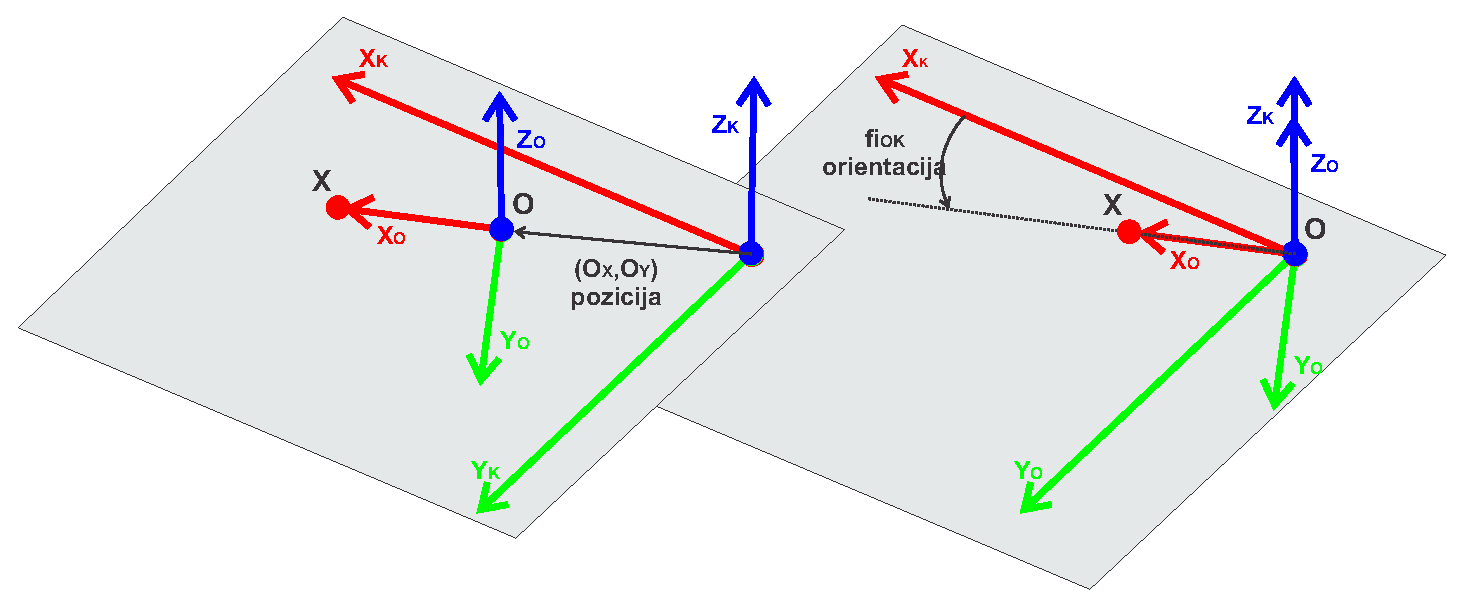
\includegraphics[width=0.85\textwidth]{/Eps/22_Lega_glede_na_kamero.eps}
    \vspace{-0.3cm}
    \caption{Lega koordinatnega sistema objekta v koordinatnem sistemu kamere}
    \label{fTransfOK}
\end{figure}

\noindent %
\textbf{\underline{Določitev matrike KamRef}} %

\vspace{0.3cm}%
Da lahko s pomočjo robotskega vida z robotom prijemamo objekte v
vidnem polju kamere in delovnem prostoru robota, je potrebno lego
objektov definirati v referenčnem koordinatnem sistemu robota. Glede
na enačbo \ref{eEqSimple} za izračun željene lege objekta v
referenčnem koordinatnem sistemu robota, potrebujemo še
\textbf{transformacijsko matriko KamRef}.
\\
\\
\noindent %
\textbf{Postopek za določitev matrike KamRef} %
\vspace{0.1cm}\\
\begin{mdframed}[backgroundcolor=green!20, shadow=true,roundcorner=8pt]
%\begin{tikzpicture}
%    \node [fill=green,rounded corners=5pt] {
%    \begin{minipage}{0.93\textwidth}
        \vspace{0.1cm}
Lega objekta oziroma koordinatnega sistema objekta je zapisana v
transformacijski matriki \textbf{ObjKam}. Za določitev lege
koordinatnega sistema kamere v referenčnem koordinatnem sistemu
robota ni mogoče najti postopka, ki bi lego določil, kot smo to
storili za lego objekta v koordinatnem sistemu kamere. Izkaže se, da
lahko postopek za določitev lege objekta v koordinatnem sistemu
kamere, v rahlo spremenjeni obliki, uporabimo za določitev matrike
\textbf{VrhRef}. Ta ob prijemu objekta predstavlja lego objekta v
referenčnem koordinatnem sistemu robota. Na ta način lahko z
izračunom določimo matriko \textbf{KamRef}, ki predstavlja lego
kamere v referenčnem koordinatnem sistemu robota.
        \vspace{0.1cm}
%    \end{minipage}
%    };
%\end{tikzpicture}
\end{mdframed}

\begin{figure}[!h]
    \center
    \includegraphics[width=0.4\textwidth]{/Eps/23_Konica.eps}
    \vspace{-0.3cm}
    \caption{V ustje robota nameščena konica, ki smo jo pozicionirali v središče točke O}
    \label{fKonica}
\end{figure}
\begin{enumerate}

\item[1)] V Epson RC+ okolju v mapi Projects\textbackslash odprite že pripravljen projekt z imenom \textbf{Epson\_kalibracija}.

\item[2)] Z ukazom \textit{Run -> Start -> Start main} projekt prevedete in zaženete.

\item[3)] Robot pobere kalibracijsko konico in se premakne do točke \emph{O}(\emph{O}$_x$, \emph{O}$_y$). Koordinate točke v World koordinatnem sistemu (Slika \ref{fUkaziPremikanjeRobota}) se izpišejo v konzoli.

\item[4)] S pritiskom na ukaz \textit{Continue} robota premaknete na točko \emph{X}(\emph{X}$_x$, \emph{X}$_y$). Koordinate točke v World koordinatnem sistemu (Slika \ref{fUkaziPremikanjeRobota}) se zopet izpišejo v konzoli.

\item[5)] S ponovnim pritiskom na ukaz \textit{Continue} robotu ukažete, da odloži kalibracijsko konico.

\item[6)] Odčitana točka \emph{O} predstavlja \textbf{pozicijo}
koordinatnega sistema objekta v referenčnem koordinatnem sistemu
robota (Slika \ref{fTransfOR}, levo). \textbf{Orientacijo}
koordinatnega sistema objekta v referenčnem koordinatnem sistemu
robota pa določa kot (fiOR) med osema \emph{X}$_R$ in \emph{X}$_O$
(Slika \ref{fTransfOR}, desno).

\begin{figure}[h]
    \center
    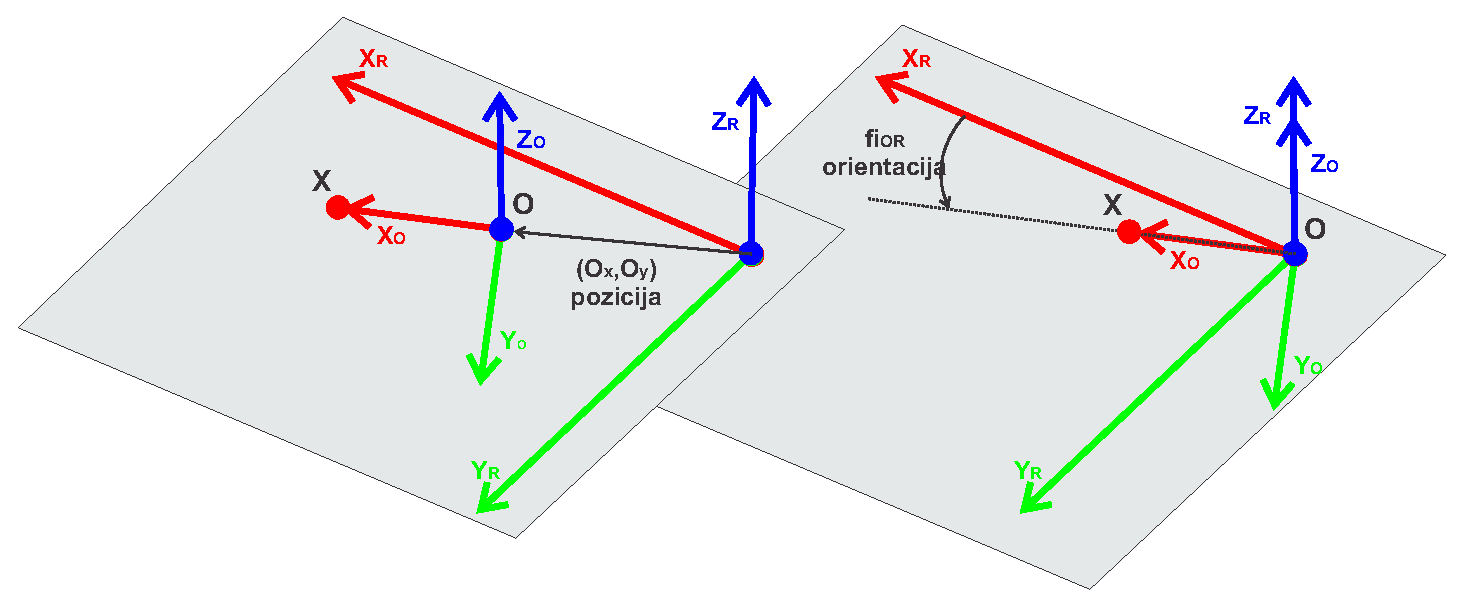
\includegraphics[width=0.85\textwidth]{/Eps/24_Lega_glede_na_bazo.eps}
    \vspace{-0.3cm}
    \caption{Lega koordinatnega sistema objekta v referenčnem koordinatnem sistemu robota}
    \label{fTransfOR}
\end{figure}

\item[7)] V okolju Matlab je že odprta datoteka
\textbf{zamaski2.m}, zato nadaljujete: \\%
\\
\small
\textcolor[rgb]{0.50,0.50,0.50}{\texttt{$\%$ V ustrezna polja vpišemo prebrane vrednosti koordinate}} \\%
\textcolor[rgb]{0.50,0.50,0.50}{\texttt{$\%$ O(O$_x$,O$_y$) in X(X$_x$,X$_y$).}} \\%
\texttt{Ox$\_$r = \emph{vpišemo prebrano koordinato};}  \\%
\texttt{Oy$\_$r = \emph{vpišemo prebrano koordinato};}  \\%
\texttt{Xx$\_$r = \emph{vpišemo prebrano koordinato};}  \\%
\texttt{Xy$\_$r = \emph{vpišemo prebrano koordinato};}  \\%
\\
\textcolor[rgb]{0.50,0.50,0.50}{\texttt{$\%$ Izračunamo kot zasuka koordinatnega sistema Objekta}} \\%
\textcolor[rgb]{0.50,0.50,0.50}{\texttt{$\%$ glede na referenčni k.s. (Slika \ref{fTransfOR}, desno).}} \\%
%\texttt{fiOR = atan2( (Xy$\_$r - Oy$\_$r ) , (Xx$\_$r - Ox$\_$r ) );} \\ %
\texttt{fiOR = \emph{... TUKAJ ZAPIŠETE PRAVILNO KODO};} \\ %
\\
\textcolor[rgb]{0.50,0.50,0.50}{\texttt{$\%$ Zapišemo transformacijsko matriko Vrh- translacija}} \\%
\textcolor[rgb]{0.50,0.50,0.50}{\texttt{$\%$ D(Ox$\_$r, Oy$\_$r) in rotacija okrog osi Z za kot fiOR.}} \\%
\texttt{VrhRef = \emph{... TUKAJ ZAPIŠETE PRAVILNO KODO};} \\ %
%\texttt{VrhRef = [cos(fiOR), -sin(fiOR), 0, Ox$\_$r; sin(fiOR), cos(fiOR),\\\hspace*{1.7cm} 0, Oy$\_$r; 0, 0, 1, 0; 0, 0, 0, 1 ];} \\ %

\normalsize %
Zapis v matrični obliki izgleda tako:
\\
\begin{equation}
    \textbf{VrhRef} =
    \begin{bmatrix}
        \textbf{cos(fiOR)}  &   \textbf{-sin(fiOR)}   &    \textbf{0}  &   \emph{Ox$\_$r}    \\%
        \textbf{sin(fiOR)}  &   \hspace{0.1cm} \textbf{cos(fiOR)}   &    \textbf{0}  &   \emph{Oy$\_$r}    \\%
        \textbf{0}              &   \textbf{0}                &    \textbf{1}  &   \emph{0}    \\%
        0              &   0                &    0  &   1     \\%
    \end{bmatrix}
    \label{eVrhRef}
\end{equation}
\\
\begin{mdframed}[backgroundcolor=blue!20, shadow=true,roundcorner=8pt]
%\begin{tikzpicture}
%    \node [fill=blue,rounded corners=5pt] {
%    \begin{minipage}{0.93\textwidth}
        \vspace{0.1cm}
Enačba \ref{eVrhRef} predstavlja transformacijsko matriko
\textbf{VrhRef} in opisuje lego objekta oziroma koordinatnega
sistema objekta v referenčnem koordinatnem sistemu robota.
        \vspace{0.1cm}
%    \end{minipage}
%    };
%\end{tikzpicture}
\end{mdframed}

\item[8)] V tem trenutku sta določeni obe transformaciji \textbf{ObjKam} in
\textbf{VrhRef}, zato lahko po spodnjem postopku izračunamo lego
koordinatnega sistema kamere v referenčnem koordinatnem sistemu
robota, ki jo predstavlja transformacijska matrika \textbf{KamRef}.
Izhodišče je enačba \ref{eEqSimple}.

\vspace{0.4cm} %

\noindent %
\begin{mdframed}[backgroundcolor=green!20, shadow=true,roundcorner=8pt]
%\begin{tikzpicture}
%    \node [fill=green,rounded corners=5pt] {
%    \begin{minipage}{0.94\textwidth}
        \vspace{0.1cm}
        \center
        \textbf{VrhRef = KamRef $\bullet$  ObjKam} \emph{$/$ z desne množimo z \textbf{(ObjKam)$^{-1}$}}\\ %
%        \textbf{EndEff = T$\_$cam2ref $\bullet$ T$\_$obj2cam $\bullet$ T$\_$grip2obj}\\ %
        \vspace{0.2cm}
        \textbf{VrhRef $\bullet$ (ObjKam)$^{-1}$ = KamRef $\bullet$ ObjKam $\bullet$ (ObjKam)$^{-1}$}\\ %
        \vspace{0.2cm}
        \textbf{KamRef = VrhRef $\bullet$ (ObjKam)$^{-1}$}\\ %
        \vspace{0.1cm}
%    \end{minipage}
%    };
%\end{tikzpicture}
\end{mdframed}
\vspace{0.0cm} %

V .m datoteko dopišete potrebne vrstice. \\ %
\\
\small
\textcolor[rgb]{0.50,0.50,0.50}{\texttt{$\%$ Zapišemo izračun transformacije KamRef}} \\%
\texttt{KamRef = \emph{... TUKAJ ZAPIŠETE PRAVILNO KODO};}  \\% ... TUKAJ ZAPIŠETE KODO;
\\
%\texttt{KamRef = VrhRef * inv(ObjKam);}  \\% ... TUKAJ ZAPIŠETE KODO;
\normalsize %

\item[9)] Ukaz \textbf{extobject2} vam bo vrnila spremenljivko \textbf{centers} v kateri se nahajajo koordinate zamaškov v enotah pixel (slikovni elementi), ki jih je potrebno pretvoriti v enote mm (milimetri). Koordinate zamaškov v enotah mm se shrani v spremeljivko \textbf{obj}.

\small
\textcolor[rgb]{0.50,0.50,0.50}{\texttt{$\%$ Središča objektov na sliki pretvorimo v metrične enote}} \\%
\texttt{obj = \emph{... TUKAJ ZAPIŠETE PRAVILNO KODO};} \\ %
\\

\normalsize %
\item[10)]  Sedaj je potrebno v izračunati matriko \textbf{VrhRef} v kateri so zapisane koordinate zamaškov v koordinatnem sistemu robota. %

~\\
\textcolor[rgb]{0.50,0.50,0.50}{\texttt{$\%$ Določitev koordinat prepoznanih objektov v referenčnem}} \\%
\textcolor[rgb]{0.50,0.50,0.50}{\texttt{$\%$ koordinatnem sistemu. Ker imamo opraviti samo s pozicijami}} \\%
\textcolor[rgb]{0.50,0.50,0.50}{\texttt{$\%$ središč pokrovčkov, ni potrebno izvajati rotacij. Zato}} \\%
\textcolor[rgb]{0.50,0.50,0.50}{\texttt{$\%$ transformacijske matrike vsebujejo samo translacijski del.}} \\%
\texttt{for ii = 1:size(centers,1)} \\ %
%\hspace*{0.2 cm}\texttt{ObjKam = [1,0,0,obj(ii,1); 0,1,0,obj(ii,2); 0,0,1,Z; 0,0,0,1];} \\ %
%\hspace*{0.2 cm}\texttt{VrhRef(:,:,ii) = KamRef * ObjKam;} \\ %
\hspace*{0.2 cm}\texttt{ObjKam = \emph{... TUKAJ ZAPIŠETE PRAVILNO KODO};} \\ %
\hspace*{0.2 cm}\texttt{VrhRef(:,:,ii) = \emph{... TUKAJ ZAPIŠETE PRAVILNO KODO};} \\ %
\texttt{end} \\ %
\\
\textcolor[rgb]{0.50,0.50,0.50}{\texttt{$\%$ Iz serije transformacijskih matrik Vrh izluščimo samo}} \\%
\textcolor[rgb]{0.50,0.50,0.50}{\texttt{$\%$ koordinate središč zamaškov v referenčnem k.s.}} \\%
\texttt{koord$\_$zamaskov;} \\ %

\normalsize %
\item[11)]  \textbf{Datoteko zamaski2.m shranimo in preverimo kalibracijo:} %

\end{enumerate}
\normalsize

\begin{mdframed}[backgroundcolor=red!20, shadow=true,roundcorner=8pt]
\begin{itemize}
  \item \textbf{Asistent naj iz mizice odstrani kalibracijsko ploščo in na mizico postavi tri zamaške.}
  \item \textbf{Zamaški naj se nahajajo v kotih, kjer so na kalibracijski mizici kalibracijske točke.}
\end{itemize}
\end{mdframed}

Kalibracijo preverite tako, da z ukazom \\

\vspace{-0.3cm}%
\textbf{$\gg$ extobject2} \verb"Enter"\\ %\Enter
\vspace{-0.1cm}%

odprete okno za zajem slike zamaškov. S ponovnim pritiskom tipke \verb"Enter" sliko zajamete. Z ukazom  \\

\vspace{-0.3cm}%
\textbf{$\gg$ zamaski2} \verb"Enter" \\%\Enter
\vspace{-0.1cm}%

se izračunajo in izpišejo koordinate zamaškov v globalnem koordinatnem sistemu. Izpisane koordinate primerjate s pozicijami kalibracijskih točk, ki ste jih dobili v prejšnjem postopku. Koordinate se morajo približno ujemati ($\pm1mm$).

\vspace{-0.2cm}
\subsection{Koraki za zagon}
\vspace{0.3cm} %

\begin{mdframed}[backgroundcolor=red!20, shadow=true,roundcorner=8pt]
\begin{itemize}
  \item \textbf{Asistent naj na mizico postavi več zamaškov.}
  \item \textbf{Med izvajanjem mora biti asistent ves čas pri robotu}
\end{itemize}
\end{mdframed}

\begin{enumerate}


\item[1)] \textbf{Vsi postopki določanja
transformacijskih matrik ObjKam in KamRef ter vse vrstice programska
kode v datoteki zamaski2.m morajo biti opravljeni oziroma zapisani!} \\%

\item[2)] \textbf{V vidno polje kamere postavite nekaj zamaškov}
(recimo 7), še prej pa odstranite kalibracijsko konico, umaknete
robot iz vidnega področja kamere in odstranite list s
koordinatnim sistemom objekta. \\ %

\item[3)] V Matlab ukazni vrstici zaženete: \\ %
%\vspace{-0.1cm} %
\textbf{$\gg$ extobject2} \verb"Enter" \\ %%\Enter


Odpre se okno kamere z živo sliko za boljše pozicioniranje zamaškov.
Ko ste s pozicijo zamaškov zadovoljni, pritisnete \verb"Enter". čez čas se%%\Enter
v ukazni vrstici okolja Matlab izpiše število razpoznanih objektov
in izriše se slika \ref{fRazbraniZamaski}. \textbf{če niste
zadovoljni z razpoznavo objektov, ta korak ponovite.} %

\begin{figure}[!h]
    \center
    \includegraphics[width=0.7\textwidth]{/Eps/25_Razbrani_zamaski.eps}
    \vspace{-0.3cm}
    \caption{Iz zajete slike razbrani zamaški ter označena njihova središča}
    \label{fRazbraniZamaski}
\end{figure}

\item[4)] V ukazni vrstici okolja Matlab poženete datoteko(\emph{zamaski2.m}).  \\ %

%\vspace{-0.3cm} %
\textbf{$\gg$ zamaski2} \verb"Enter" \\ %%\Enter
\vspace{-0.1cm} %

\item[5)] V Epson RC+ okolju v mapi Projects$\backslash$ odprete že pripravljen projekt z imenom \textbf{Epson$\_$kamera}. \\ %

\begin{mdframed}[backgroundcolor=red!80, shadow=true,roundcorner=8pt]
%\begin{tikzpicture}
%    \node [fill=red,rounded corners=5pt] {
%    \begin{minipage}{0.93\textwidth}
        \vspace{0.1cm}
 \textbf{Ob zagonu programa poskrbite, da robot deluje %
 z nižjo močjo in njegova hitrost gibanja naj bo le 10$\%$ (prvi dve vrstici programa).}
 \\
 \\
\hspace*{3.5cm}\textcolor[rgb]{1.00,1.00,0.00}{\emph{\textbf{$\#$define dPower Low}}} \\ %
\hspace*{3.5cm}\textcolor[rgb]{1.00,1.00,0.00}{\emph{\textbf{$\#$define dSpeedAccelProcent 10}}} \\ %
        \vspace{-0.3cm}
%    \end{minipage}
%    };
%\end{tikzpicture}
\end{mdframed}
\vspace{0.3cm}

\item[6)] S tipko F5 projekt prevedete
(Slika \ref{fZaganjanjePrograma}) in ga zaženete s klikom na gumb \textbf{Start tcpipcomm}. %

% ********************************************************************
\vspace{0.3cm}
\begin{mdframed}[backgroundcolor=red!80, shadow=true,roundcorner=8pt]
%\begin{tikzpicture}
%    \node [fill=red,rounded corners=5pt] {
%    \begin{minipage}{0.93\textwidth}
        \vspace{0.1cm}
        \center
        \large
\textcolor[rgb]{1.00,1.00,0.00}{\LARGE\textbf{OPOZORILO!}}\\ %
\textcolor[rgb]{1.00,1.00,0.00}{\large Pred zagonom programa je
potrebno zagotoviti, da v delovnem prostoru ni osebe ali predmeta, s
katerim bi lahko robot trčil.} \\ %
        \vspace{0.1cm}
%    \end{minipage}
%    };
%\end{tikzpicture}
\end{mdframed}
\vspace{0.3cm}
\item[7)] V ukazni vrstici okolja Matlab izvršite ukaz (štarta premikanje robota): \\ %

\vspace{-0.1cm} %
\textbf{$\gg$ zamaski$\_$tcp} \verb"Enter" \\ %%\Enter
\normalsize
% ********************************************************************
\end{enumerate}
     % Epson vid
% -*- TeX:SI -*-
% slovene sub-mode for spell check

%\Large\textbf
\chapter{{KUKA Youbot mobilna platforma}}

\vspace{-1.5cm}

\begin{mdframed}[backgroundcolor=green!20, shadow=true,roundcorner=8pt]
\vspace{-0.35cm}
\section{Cilji vaje}
\begin{itemize}
\item spoznavanje z vodenjem mobilne platforme youBot Kuka
\item uporaba znanja pridobljenega na predavanjih o homogenih transformacijah med različnimi koordinatnimi sistemi
\item uporaba video sistema za vodenje mobilne robotske platforme
\item spoznavanje okolja Matlab Simulink za preračun homogenih transformacij, vodenje platforme in načrtanje posameznih korakov za izvedbo večstopenjeske naloga pobiranja in prenašanja različnih objektov


\end{itemize}
\end{mdframed}



\section{Uvod}
 Industrijska robotika je v stalnem porastu in še za vrsto let vnaprej lahko rečemo, da bo vsako novo leto tudi leto z novim porastom števila industrijskih robotskih aplikacij in nameščenih robotov v industrijskem okolju. Nameščeni oziroma pričvrščeni na svoje mesto v proizvodnem procesu so sposobni opravljati naloge, ki zahtevajo natančnost in hitro izvajanja ciklov. Precejšen del industrije je močno odvisen od industrijskih robotov. Kljub temu pa imajo eno bistveno pomanjkljivost, in to je pomanjkanje mobilnosti. Pritrjen manipulator ima omejen delovni prostor, ki je določen s kinematično strukturo roke in seveda z mestom kjer je pritrjen. Mobilni roboti imajo seveda to prednost, da se lahko pomikajo po prostoru in je njihov delovni prostor precej manj omejen in veliko večji. Seveda pa se s tem odpre celo novo področje vodenja robotov, kjer je glavni problem določanje lege robota v prostoru. če je za določenje lege robota v prostoru v primeru industrijskih robotov dovolj en enkoder v vsakem sklepu, pa je za določanje lege v prostoru pri mobilnih robotih potrebno imeti na voljo večje število senzorjev.

Mobilni roboti odpirajo celo vrsto novih možnosti in postajo zanimivi tudi za industrijsko okolje, še mnogo bolj zanimivi pa za okolje v katerem se gibljemo tudi mi sami, dasiravno ima človeška domišljija močno nerealna pričakovanja česa vse naj bi bili mobilni roboti sposobni.
KUKA youBot je mobilna platforma z robotsko roko, ki jo je razvilo nemško podjetje KUKA, ki izdeluje industrijske robote.

KUKA youBot je namenjen za izobraževanje in raziskave na področju mobilne robotike. Zaradi tega se KUKA youBot ponaša z odprto krmilniško arhitekturo, kar omogoča dostop do vseh nivojev strojne opreme in vodenja. Delo s KUKA youBot-om torej zahtevo vsaj osnovno znanje iz robotike in vodenja naprav, kar je seveda nadvse primerno za uporabo KUKA youBot platforme pri vajah pri predmetu Osnove robotike.
KUKA youBot je sestavljena iz dveh poglavitnih delov:
\begin{itemize}
\item KUKA youBot vsesmerna mobilna platforma (ang. omni-directional mobile platform) je sestavljena iz ohišja, štirih vsesmernih švedskih koles (ang. mecanum wheels), štirih motorjev za pogon koles, osebnega računalnika in seveda potrebnih elektronskih vezij. Uporabniki lahko bodisi zaganjajo algoritme vodenja na računalniku, ki se nahaja na platformi, ali pa na oddaljenem računalniku.
\item KUKA youBot antropomorfna robotska roka ima 5 prostostnih stopenj in dvoprstno prijemalo. če je robotska roka nameščnea na mobilno platformo, vodenje roke poteka prek računalnika na mobilni platformi. Roko je možno voditi tudi brez platforme z navadnim osebnim računalnikom preko Ethernet povezave.
\end{itemize}

Na platformo je mogoče montirati še vrsto senzorjev kot so Kinect 3D Camera, laserski merilec razdalje, stereo kamero, ultrazvočne merilnike razdalje, itd.

\section{Hiter pregled vaje}

Pri tej vaji boste s pomočjo KUKA youBot platforme, ki je prikazana na sliki \ref{fig:KUKA1}, igrali miselno igro Hanojski stolp.

\emph{Hanojski stolp} je miselna oziroma logična igra. Začne se s stolpom diskov, ki so naloženi na drug drugega od največjega spodaj do najmanjšega zgoraj, kot je prikazano na sliki \ref{fig:han_tower}. Cilj je prenesti diske na drugo mesto, kjer morajo biti postavljeni v istem vrstnem redu, pri čemer imamo na voljo samo eno vmesno odlagališče. Pri reševanju moramo upoštevati naslednja pravila:

\begin{itemize}
\item Diske premikamo posamično.
\item Poteza zajema premik zgornjega diska na drugo mesto oziroma premik na večji disk.
\item Nikdar ne smemo postaviti večjega diska na vrh manjšega diska.
\end{itemize}

\begin{figure}[h]
\centering \resizebox{6cm}{!}{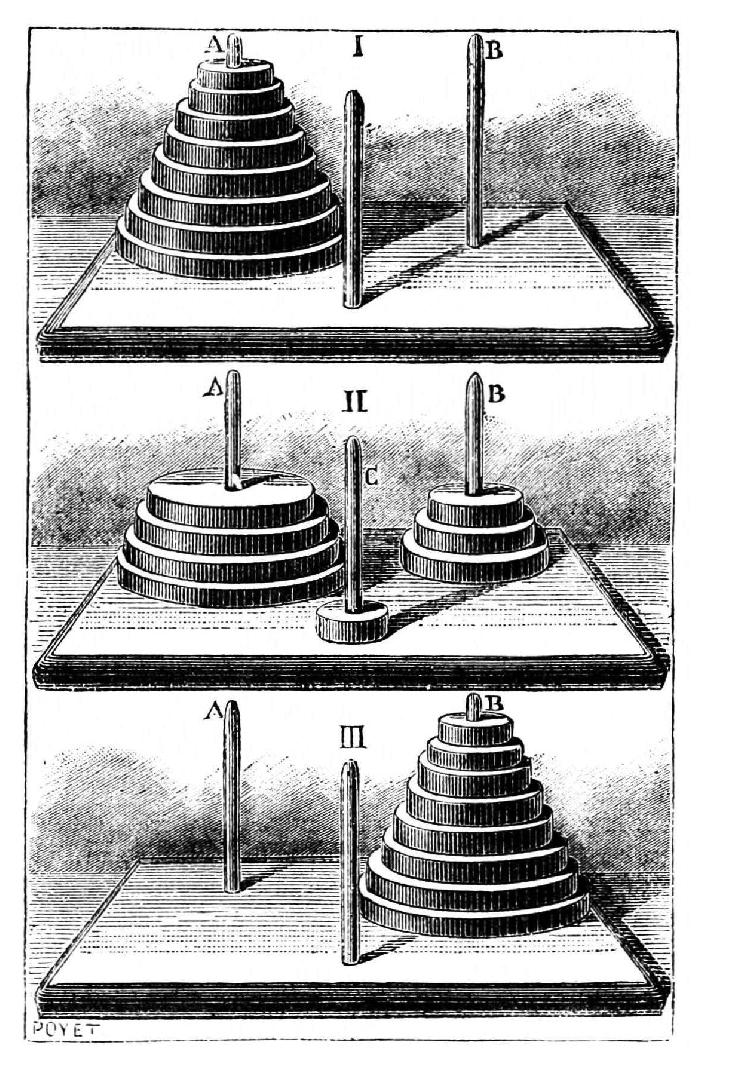
\includegraphics[draft=false]{PSM_V26_D464_The_tower_of_hanoi.eps}}
\caption{Igra Hanojski stolp z diski različnih velikosti.}
\label{fig:han_tower}
\end{figure}

Za reševanje igre z robotom se namesto diskov uporabja kocke. Med seboj se razlikujejo po barvi vrhnje kocke, ki je namenjen za prijem. Vse kocke so enako velike, največji disk prestavljajo tri rumene kocke, naslednji disk dve rdeči kocki, najmanjši disk pa ena zelena kocka. Igro se torej igra kot bi imel tri diske različnih velikosti.

Za izvedbo naloge uporabljamo tri lokacije, začetna lokacija kock, vmesno odlagališče, ter končna lokacija. Začetno postavitev naloge prikazujeta sliki \ref{fig:AllFrames} in \ref{fig:AllTocke}. Cilj naloge je, da s pomočjo robota prestavimo kocke iz začetne na končno lokacijo po naslednjih pravilih: barvne oznake so zelena, rdeča in rumena. Rumenih kock ne smemo nikoli postaviti pred rdečimi oziroma zelenimi kockami, pravtako  rdečih kock ne smemo nikoli prstaviti pred zelenimi. Vedno smemo prestavljati samo kocke ene barve, ker predstavljajo en disk, v vrsti morajo seveda ležati le kocke istih barv.  Pravilni vrstni red postavitve je prikazan na slikah \ref{fig:AllFrames} in \ref{fig:AllTocke}.

Koraki za izvedbo naloge so sledeči:
\begin{enumerate}
\item Pretvorba iz koordinatnega sistema kamere v globalni koordinatni sistem.
    \begin{enumerate}
    \item Odprava perspektive pri zajemanju pozicije objektov s pomočjo kamere.
    \item Transformacija leg objektov iz koordinatnega sistema kamere v globalni koordinatni sistem.
    \end{enumerate}
\item Priprava preprostega regulatorja za vodenje mobilne platforme v globalnem koordinatnem sistemu.
\item Programiranje zaporedja operacij za nalogo "Hanojski stolp".

\end{enumerate}


\section{KUKA youBot vsesmerna mobilna platforma}

KUKA youBot platforma je vsesmerna mobilna platforma s štirimi švedskimi kolesi. Vsesmerno gibanje ji mogočajo švedska kolesa (poimenovana po narodnosti izumitelja teh koles Bengta Ilona, v literaturi so pogosto imenovana tudi Mecanum kolesa), vsako kolo ima svoj motor. Platforma se tako lahko giblje naprej-nazaj, levo-desno in rotira okoli svoje osi. Platforma ima torej 3 prostostne stopnje.
Slika 1 prikazuje koordinatni sistem na KUKA youBot vsesmerni mobilni platformi. Os x kaže v smeri naprej (na sprednjem delu platform je pritrjena robotska roka, na zadnjem delu pa je nameščena miza za odlaganje predmetov), y os kaže v smeri levo, z os pa navzgor. \vspace{1cm}

\begin{figure}[h]
\centering \resizebox{10cm}{!}{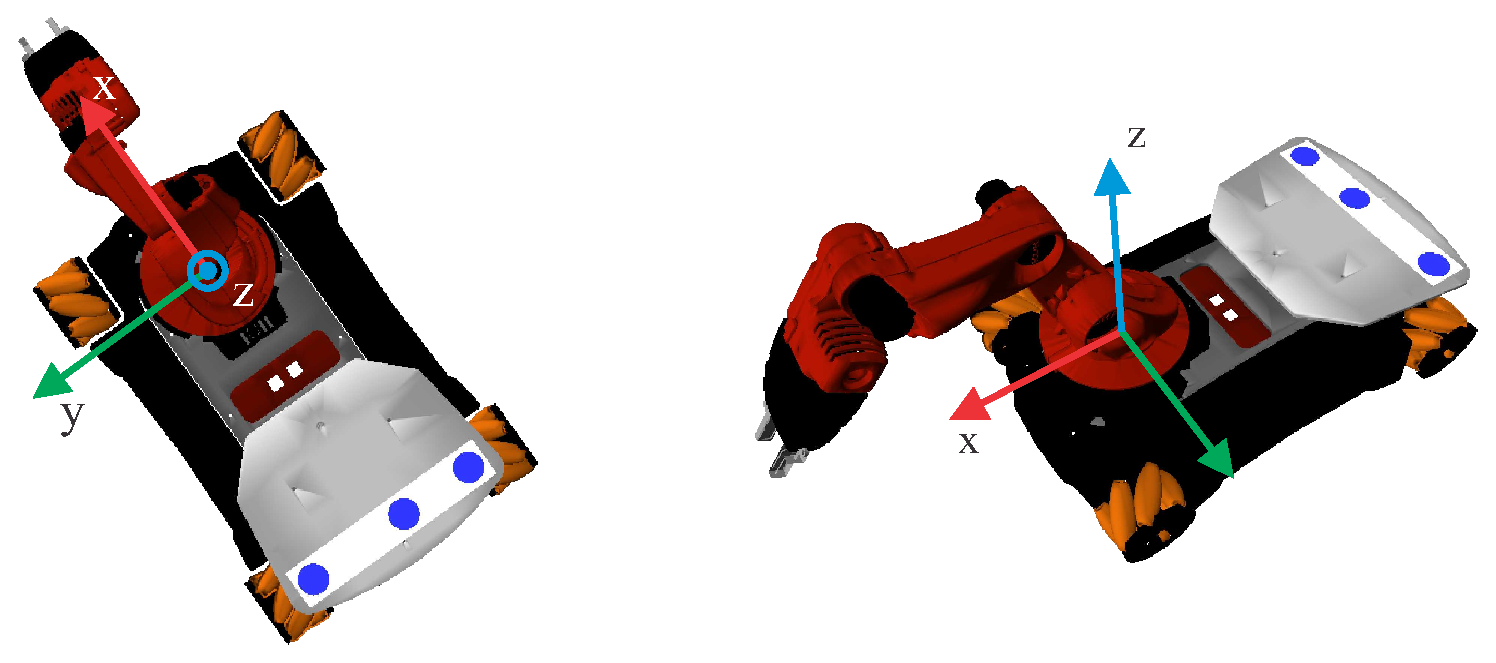
\includegraphics[draft=false]{KUKAFrame-4.eps}}
\caption{KUKA youBot s koordinatnim sistemom.}
\label{fig:KUKA1}
\end{figure}

Platformo vodimo tako, da podamo vektor treh hitrosti $\begin{bmatrix} v_x \\ v_y \\ \omega_z \end{bmatrix}$:
\begin{itemize}
\item hitrost gibanja v $x$ smeri $v_x$,
\item hitrost gibanja v $y$ smeri $v_y$,
\item hitrost rotiranja okoli $z$ osu $\omega_z$.
\end{itemize}
Platforma sama ne vsebuje nobenih senzorjev, ki bi omogočali določanjene njene lege v prostoru. Za določanje lege platforme v prostoru se uporablja kamero, ki je nameščena na stropu. Z robotskim vidom je tako mogoče določiti lego platforme v prostoru. Več o tem je zapisano v podpoglavju \ref{pog:RobVid}.

\section{KUKA youBot robotska roka}

KUKA youBot robotska roka je serijski mehanizem s petimi prostostnimi stopnjami. Na koncu prijemala se nahaj dvoprstno prijemalo. Roka ima v sklepih enkoderje za merjenje kota zasuka v sklepu, vsak sklep poganjajo električni motorji, ki nima mehanskih zavor. če torej izklopimo napajanje na platformi, se bo robotska roka sesedla. Roka lahko dvigne $0.5$ $kg$ in ima dosega v horizontalni ravnini $0.54$ $m$. Koordinatni sistem platforme je namerno postavljen pod bazo robotske roke, saj se tako bazni koordinatni sistem robotske roke in platforme pokrivata. Koordinatna sistema platforme in roke sta torej ista.

\vspace{0.5cm}

\begin{table}
\caption{Lastnosti KUKA youBot robotske roke}
\begin{tabular}{|l|l|}
\hline Krmiljene osi & 5 \\
\hline Nosilnost &	0,5 kg \\
\hline Doseg &	540 mm \\
\hline Ponovljivost & 	1 mm \\ \hline
\end{tabular}
\end{table}

%\vspace{0.5cm}

\begin{table}
\caption{Obseg gibanja za posamezni sklep}
\begin{tabular}{|l|l|}
\hline Os i & $\Theta_i$ \\
\hline 1 &	+/- 169$\,^{\circ}$ \\
\hline 2 &	+90 $\,^{\circ}$/-65 $\,^{\circ}$ \\
\hline 3 & 	+146 $\,^{\circ}$/-151 $\,^{\circ}$ \\
\hline 4 & 	+/-102 $ \,^{\circ}$ \\
\hline 5 & 	+/-167 $ \,^{\circ}$ \\ \hline
\end{tabular}
\end{table}

\vspace{0.5cm}

\begin{figure}[h]
\centering \resizebox{10cm}{!}{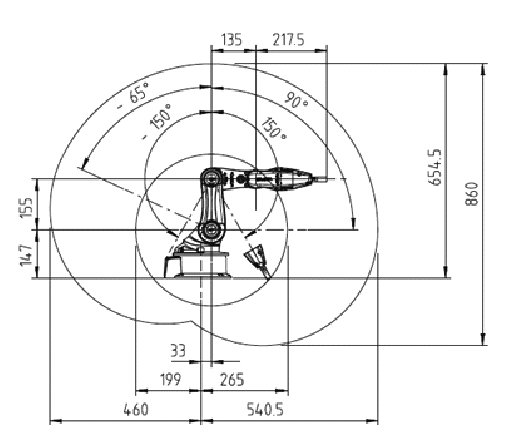
\includegraphics[draft=false]{envelope.eps}}
\caption{Delovni prostor roke youBot.}
\end{figure}

Robotsko roko vodimo s pomočjo inverzne kinematike, ki je v sheme vodenja že vključena. Vhod v inverzno kinematiko je vektor 5 vrednosti (glej sliko \ref{fig:RokaKoor}):
\begin{itemize}
\item vektor treh vrednosti $x$, $y$, $z$, ki predstavljajo željeno pozicijo vrha v koordinatnem sistemu platforme,
\item kot $\theta$, ki predstavlja kot zasuka predzadnjega segmenta robotske roke,
\item zapri/odpri prijemalo.
\end{itemize}

\begin{figure}[h]
\psfrag{th}[][l][3.0][0]{$\theta$}
\psfrag{p}[][l][3.0][0]{$p$}
\psfrag{x}[][l][3.0][0]{$x$}
\psfrag{y}[][l][3.0][0]{$y$}
\psfrag{z}[][l][3.0][0]{$z$}
\centering \resizebox{10cm}{!}{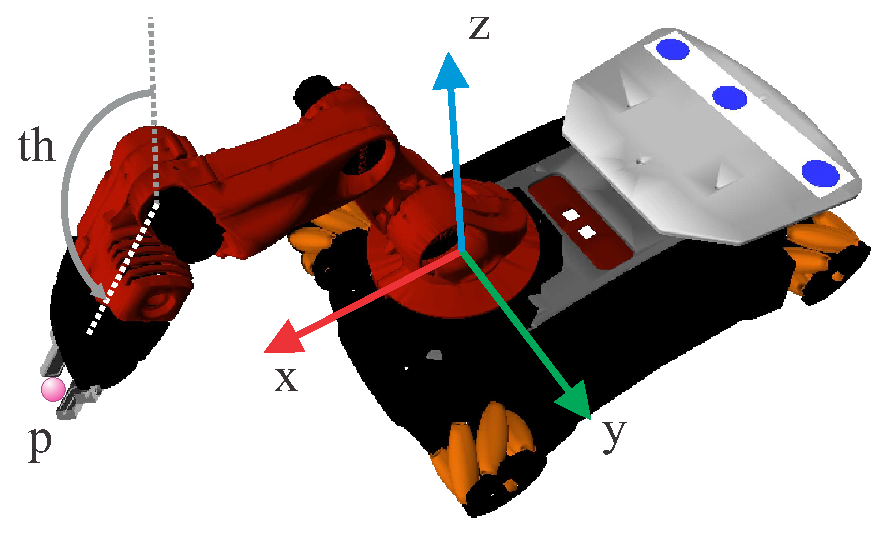
\includegraphics[draft=false]{KUKAFrame-3.eps}}
\caption{Robotksa roka KUKA. Točka $p$ predstavlja točko pomika vrha roke v koordinatnem sistemu platforme, kot $\theta$ pa zasuka predzadnjega segmenta roke.}
\label{fig:RokaKoor}
\end{figure}


\section{Robotski vid za določanje lege platforme}\label{pog:RobVid}

Za zajem slike se uporablja spletno kamero Logitech HD C920, ki omogoča zajem videa z ločljivostjo 1280x720 slikovnih pik (ang. pixel) in široki kot pogleda $85$ stopinj. Kamera je nameščena na višino $2.81$ metra, kar omogoča vidno polje $3.84$ x $2.16$ metra. To je torej delovni prostor platforme.
Zajeta slika se obdela v programskem okolju MATLAB z orodjem Image Processing Toolbox. Orodje Image Acquisition Toolbox omogoča direktni dostop do kamere in s tem tudi zajem videa oziroma posameznih slik.


\begin{figure}[h]
\psfrag{x}[][l][2.0][0]{$x_C$}
\psfrag{y}[][l][2.0][0]{$y_C$}
\psfrag{z}[][l][2.0][0]{$z_C$}
\centering \resizebox{10cm}{!}{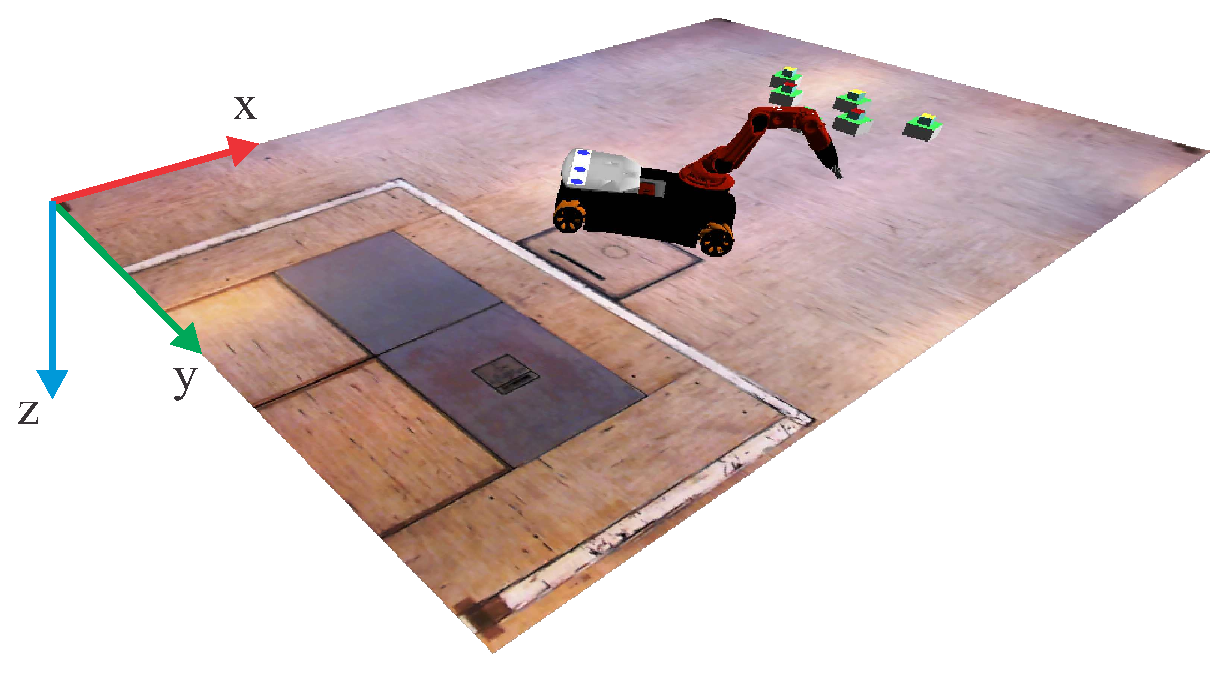
\includegraphics[draft=false]{cameraFrame.eps}}
\caption{Vidno polje kamere, ki določa delovni prostor platforme, in koordinatni sistem kamere.}
\end{figure}

Program za obdelavo slike je namenjen iskanju lege platforme in začetne lege 6 kock. Vrača $x$ in $y$ koordinato ter kot zasuka $\varphi$ za platformo in vsako od 6 kock. Na platformi se na plošči za odlaganje nahajajo tri modre pike iz katerih program za obdelavo slike določi pozicijo in orientacijo platforme. Program izračunava novo pozicijo platforme s 10 osvežitvami lege na sekundo (ang. 10 FPS), medtem ko se lego kock določi samo enkrat na začetku. Program vrača koordinati $x$ in $y$, ki sta že preračunani v metre v koordinatnem sistemu kamere. Za platformo tudi že vrača pozicijo izhodišča koordinatnega sistemom na KUKA platformi. Program najprej določi položaj posameznih treh pik, izračuna sredinsko lego med skrajnima modrima točkama in doda premik do koordnatnega sistema platfome. Kot $\varphi$ določa kot med x-osjo koordinatnega sistema kamere in x-osjo koordinatnega sistema platforme.

\begin{figure}[h]
\psfrag{x1}[][l][2.0][0]{$x_C$}
\psfrag{y1}[][l][2.0][0]{$y_C$}
\psfrag{z1}[][l][2.0][0]{$z_C$}
\psfrag{x3}[][l][2.0][0]{\color{white}$x_K$}
\psfrag{y3}[][l][2.0][0]{\color{white}$y_K$}
\psfrag{z3}[][l][2.0][0]{\color{white}$z_K$}
\psfrag{fi}[][l][2.0][0]{\color{white}$\varphi$}
\psfrag{[xK,yK]}[][r][2.0][0]{\color{white}$[\prescript{C}{}x_K,\,\,\prescript{C}{}y_K]$}
\centering \resizebox{10cm}{!}{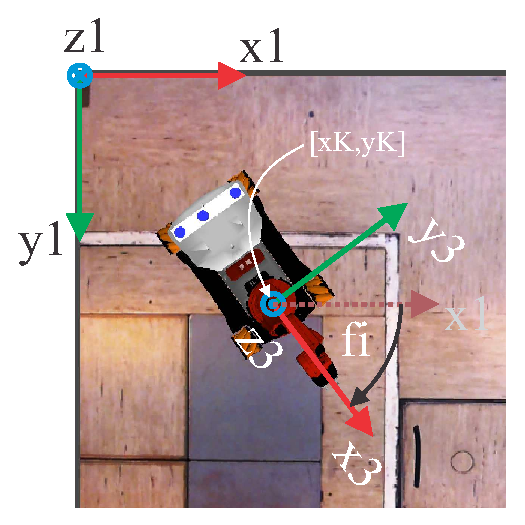
\includegraphics[draft=false]{frames-3.eps}}
\caption{Koordinatni sistem kamere cs1 in koordinatni sistem KUKE cs3.}
\end{figure}

\section{Zapis leg platforme in roke}

Kljub temu, da sta koordinatna sistema roke in platforme postavljena na isti mesti, pa se zapisa leg platforme in roke razlikujeta. Ker se platforma premika v ravnini, se za zapis pozicije platforme uporablja dve koordinati in sicer $x$ in $y$ pozicijo platforme. Platformi lahko orientacijo spreminjamo samo okoli z osi, zato za orientacijo platforme zadostuje en kot $\varphi$. Lega platforme je torej zapisana z dvema podatkoma za pozicijo ter enim za orientacijo. Lego torej zapišemo z vektorjem $[x_K, y_K, \varphi]$.
Pri robotski roki nas seveda zanima lega prijemala, ki se nahaja na koncu robotske roke. Lego prijemala zapišemo s tremi koordinatami za pozicijo $x$, $y$ in $z$, ter enim kotom $\theta$. Celoten zapis za lego torej obsega štiri podatke $[x_G, y_G, z_G, \theta]$. Za vodenje roke dodamo še peti podatek, ki določa odpiranje in zapiranje prijemala.
Koordinata z-osi nas torej pri vodenju platforme ne zanima, saj želimo platformo pripeljati v točko v ravnini. Nas pa seveda v tisti točki z koordinata zanima za vodenje roke, saj se mora roka spustiti na pravo višino za pobiranje predmeta.

\section{Zaganjanje sheme}

V ukazni vrstici z ukazom \newline \newline \verb"initall"  \newline \newline zaženete uporabniški vmesnik za vodenje KUKA platforme. Odpre se tudi simulink model za vodenje platforme. Slika \ref{fig:GUI} prikazuje uporabniški vmesnik, slika \ref{fig:model} pa simulink model. Simulink model se uporablja za poganjanje youBot platforme. 

\begin{figure}[h]
	\centering \resizebox{7cm}{!}{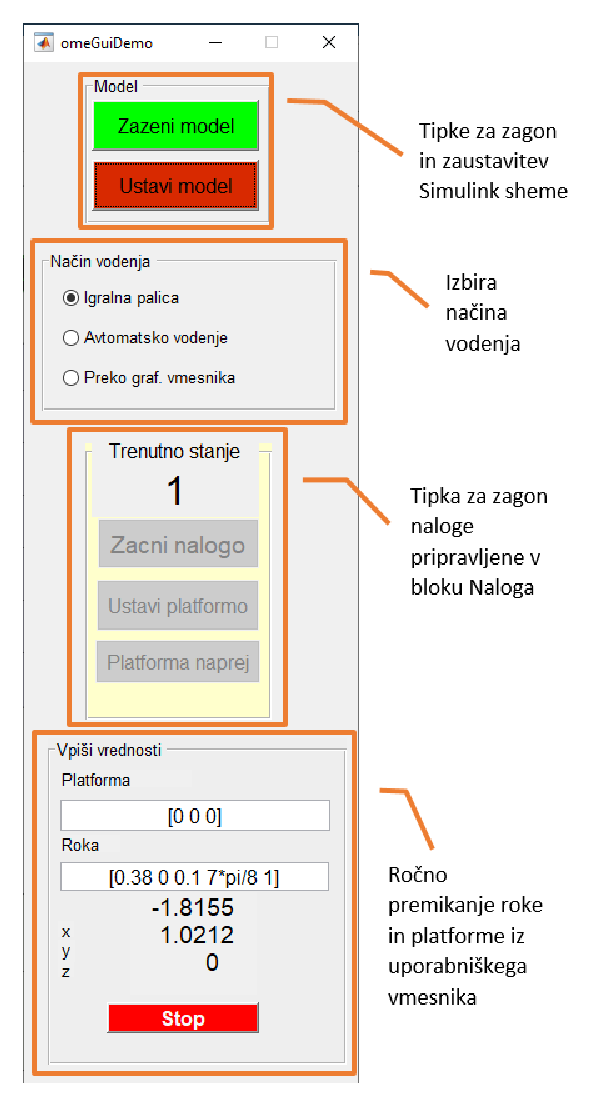
\includegraphics[draft=false]{GUI4.eps}}
	\caption{Uporabniški vmesnik za vodenje platforme.}
	\label{fig:GUI}
\end{figure}

\begin{figure}[h]
	\centering \resizebox{16cm}{!}{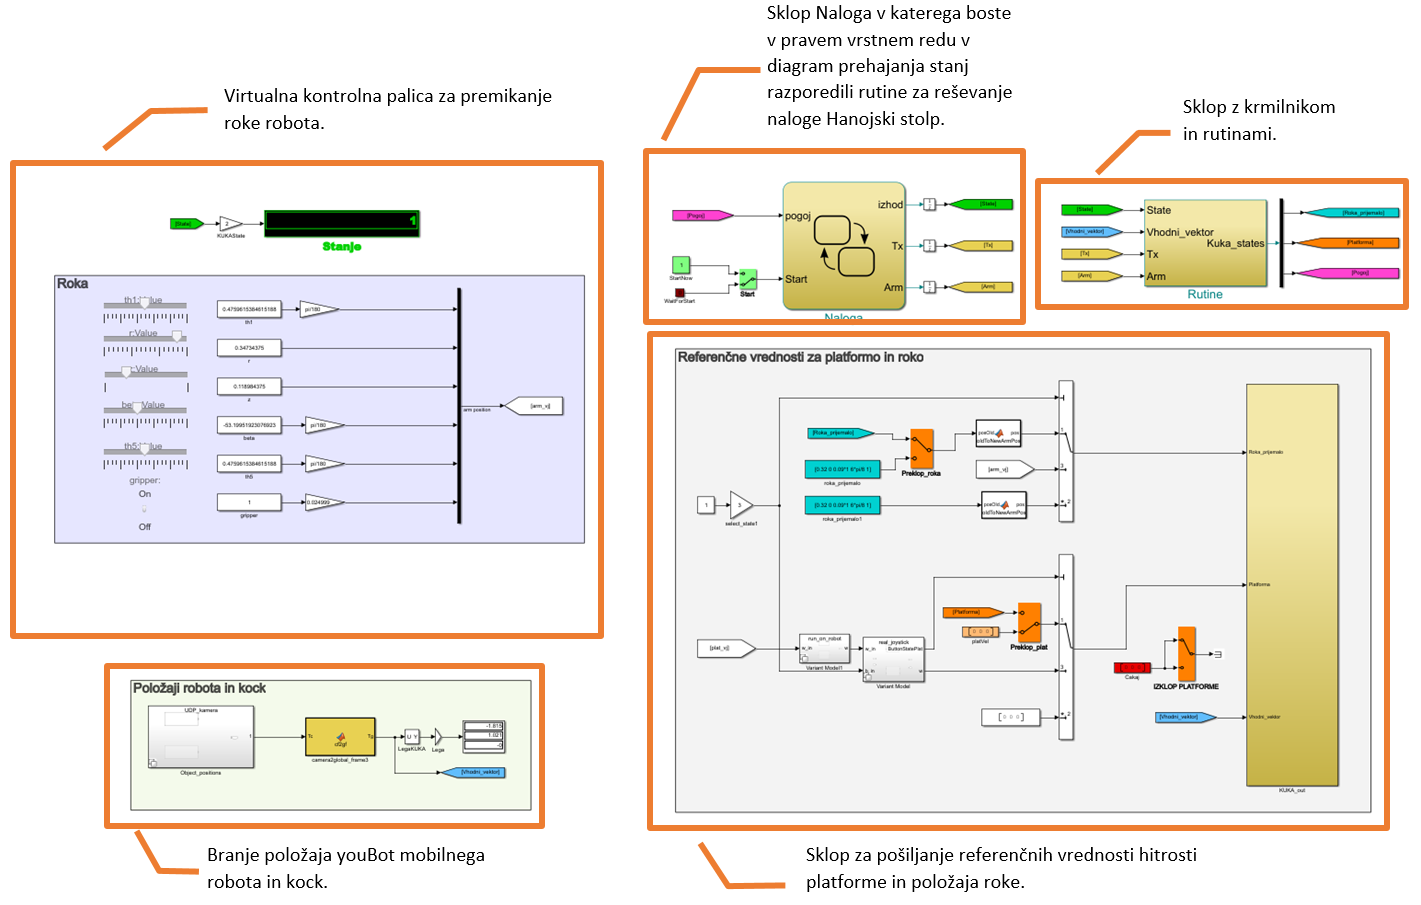
\includegraphics[draft=false]{simulink_shema4.eps}}
	\caption{Simulink model za vodenje platforme.}
	\label{fig:model}
\end{figure}

Simulnik shema, ki jo boste urejali se odpre z zagonom matlab skripte \verb|initall|. Del sheme je že vnaprej pripravljenen, v njej so z rumeno barvo označeni bloki, ki jih boste med vajo dopolnili glede na navodila v nadaljevanju skripte.

\subsection{Uporabniški vmesnik}

Uporabniški vmesnik na sliki \ref{fig:GUI} je razdeljen na več sklopov.

V sklopu \verb"Model" se nahajata gumba za zaganjanje in ustavljanje simulink  modela.
\begin{itemize}
\item Gumb \verb"Zazeni model". S pomočjo tega gumba zaženete simulink model za vodenje KUKA platforme. Ko zaženete simulink model, KUKA platforma miruje in čaka, da zaženete nalogo.
\item Gumb \verb"Ustavi model". S tem gumbom ustaviti izvajanje simulink modela.
\end{itemize}

V sklopu \verb"Način vodenja" se nahaja izbira načina vodenja mobilne platforme.
\begin{itemize}
	\item \verb"Igralna palica". Premikanje mobilne platforme s pomočjo igralne palice.
	\item \verb"Avtomatsko vodenje". Premikanje mobilne platforme preko sprogramiranega krmilnika. Zaznavanje položaja mobilne platforme poteka preko kamere na stropu. Avtomatizirano vodenje pripravite v bloku \verb|Naloga| (opisan v naslednjem poglavju).
	\item \verb"Preko graf. vmesnika". Premikanje mobilne platforme in roke preko vpisovanja željenih vrednosti hitrosti gibanja platforme in položaja roke. Vrednosti vpisujete v sklopu \verb"Vpiši vrednosti", ki je del uporabniškega vmesnika.
\end{itemize}


Sklop \verb"Trenutno stanje"
\begin{itemize}
\item Prikaz \verb"Trenutno stanje". Naloga, ki jo boste sprogramirali, je sestavljena iz posameznih podnalog, kot recimo \textit{poberi zeleno kocko}, \textit{pojdi na točko $T$}, \textit{poberi rumene kocke in jih postavi na končno mesto}, itd. Vsaka od teh podnalog ima svojo kodo, ki se izpisuje na tem mestu.
\item Gumb \verb"Zacni nalogo". Začne se izvajata sprogramirana naloga.
\item Gumb \verb"Ustavi platformo". Ta gumb izberete, ko želite začasno ustavi platformo ali izvajanje naloge. Ob kliku na gumb se referenčna hitrost za platformo postavi na vrednsot $[v_x,v_y,\omega]=[0,0,0]$. Mobilna platforma se zato ustavi, sama naloga pa še vedno teče. V primeru, da je naloga v podnalogi pobiranje kock z robotsko roko, bo roka kocke pobrala, vendar se platforma ne bo pomaknila naprej.
\item Gumb \verb"Platforma naprej". Ob kliku na gumb se referenčna hitrost za platformo postavi na vrednsot iz krmilnika za vodenje mobilne platforme in platforma se bo gibala naprej.
\end{itemize}

Sklop \verb"Vpiši vrednosti" omogoča pomikanje platforme in roke iz uporabniškega vmesnika. 

\begin{itemize}
	\item Polje \verb|Platforma|: vpišete vrednosti hitrosti za premikanje platforme. Vpišete vektor vrednosti za vodenje po osi x, osi y in rotaciji okoli osi z.
	\item Polje \verb|Roka|: vpište 5 vrednosti za postavitev roke v izbrano točko. Prve tri vrednsoti predstavljajo položaj x,y,z vrha roke, 4. vrednost je zasuk prijemala, 5. vrednost pa je vrednosti 0 za odprto prijemalo in vrednost1 za zaprto prijemalo.
	\item Prikaz položaja platforme: položaj x in y, ter rotacija platforme okoli osi z.
\end{itemize}


\newpage

\subsection{Simulink shema za vodenje platforme}

Slika \ref{fig:model} prikazuje simulink model za vodenje platforme. Glavni elementi sheme so označeni in opisani na sliki. Sklop Roka omogoča premikanje položaja robotske roke s pomočjo drsnikov.

V simulink shemi modela je najpomembnejši blok \verb"Naloga" v katerem je zapisano zaporedje ukazov, ki jih bo izvajala KUKA. S klikom na blok se odpre okno \verb"Stateflow (chart)". \verb"Stateflow (chart)" je okno za urejanje diagrama prehajanja stanj. Vsako stanje predstavlja svojo podnalogo v katero vstopite oziroma izstopite, ko je za to izpolnjen pogoj. Pogoj je izpolnjen, ko je končana posamezna podnaloga. Vsaka podnaloga ima svojo kodo, ki predstavlja stanje v katerem je celotna naloga. Seznam podnalog s kodami nalog in kodami, ko je podnaloga končana, je v tabeli \ref{tab:kodenalog}. Slika \ref{fig:stateflow1} prikazuje primer diagrama prehajanja stanj. Vsak stanje je predstavljeno z blokom, ki ima ime, vsebino in izstopni pogoj. Vsak diagram stanj, ki ga boste programirali, bo imel začetni blok \verb"Init", v katerem se bo program zadrževal, dokler ne boste v uporabniškem vmesniku kliknili na gumb \verb"Zazeni nalogo". Takrat bo izpolnjen pogoj \verb"[Start==1]" in diagram se bo prestavil v naslednje stanje. V diagramu na sliki \ref{fig:stateflow1} je to stanje z imenom \verb"Prestavi_zeleno_na_T1" in vsebino \verb"en:izhod=24;". Izvedla se bo torej rutina pobiranje zelene kocke z začetne lokacije in prestavljanja na točko $T_1$. Izstopni pogoj bloka \verb"[pogoj==124]" bo izpolnjen, ko bo KUKA prestavila zeleno kocko na točko $T_1$. Naloga se bo takrat nadaljevala z rutino s kodo \verb"25". Zadnji blok v diagramu bo blok z imenom \verb"Konec", v katerem bo ostal diagram in celotno vodenje platforme, dokler ne ugasnete simulink model.

\begin{figure}[h]
%\psfrag{x1}[][l][2.0][0]{$x_C$}
%\psfrag{y1}[][l][2.0][0]{$y_C$}
%\psfrag{z1}[][l][2.0][0]{$z_C$}
%\psfrag{x3}[][l][2.0][0]{$x_K$}
%\psfrag{y3}[][l][2.0][0]{$y_K$}
%\psfrag{z3}[][l][2.0][0]{$z_K$}
\centering \resizebox{10cm}{!}{\includegraphics[draft=false]{stateflow.eps}}
\caption{Diagram prehajanja stanj za primer preproste naloge prestavljanja zelene in rdečih kock.}
\label{fig:stateflow1}
\end{figure}

Drugi pomemben blok v simulink modelu je blok \verb"Rutine" v katerih se nahajajo bloki za vodenje platforme, ki se jih kliče iz diagrama prehajanja stanj. Bloki vsebujejo zaporedje referenc za robotsko roko in prijemalo, ter krmilnik za vodenje mobilne platforme.

\newpage

% Table generated by Excel2LaTeX from sheet 'Sheet1'
\begin{table}[htbp]
  \centering
  \caption{Seznam podnalog s kodami nalog in kodami, da je podnaloga končana.}
    \begin{tabular}{rrr}
    \toprule
          & Koda  & Pogoj izpolnjen \\
    \midrule
    Konec & 1     & N/A \\ \hline
    Primi kocko & 2     & 12 \\ \hline
    Odlozi kocko & 3     & 13 \\ \hline
    Pojdi do zelene (Z1) & 4     & 10 \\ \hline
    Pojdi do rdeče 1 (Rd1) & 5     & 10 \\ \hline
    Pojdi do rdeče 2 (Rd2) & 6     & 10 \\ \hline
    Pojdi do rumene 1 (Ru1) & 7     & 10 \\ \hline
    Pojdi do rumene 2 (Ru2) & 8     & 10 \\ \hline
    Pojdi do rumene 3 (Ru3) & 9     & 10 \\ \hline
    Pojdi na točko T10 & 10    & 10 \\ \hline
    Pojdi na točko T1 & 11    & 10 \\ \hline
    Pojdi na točko T2 & 12    & 10 \\ \hline
    Pojdi na točko T3 & 13    & 10 \\ \hline
    Pojdi na točko T4 & 14    & 10 \\ \hline
    Pojdi na točko T5 & 15    & 10 \\ \hline
    Pojdi na točko T6 & 16    & 10 \\ \hline
    Pojdi na točko T7 & 17    & 10 \\ \hline
    Pojdi na točko T8 & 18    & 10 \\ \hline
    Pojdi na točko T9 & 19    & 10 \\ \hline
    Primi in odloži kocko na platformo desno & 20    & 120 \\ \hline
    Odloži kocko s platforme desno & 21    & 121 \\ \hline
    Primi in odloži kocko na platformo levo & 22    & 122 \\ \hline
    Odloži kocko s platforme levo & 23    & 123 \\ \hline
    Pojdi po zeleno na Z1 in jo odloži na T1 & 24    & 124 \\ \hline
    Pojdi po rdeči kocki in ju odloži na točki T2 in T3 & 25    & 125 \\ \hline
    Pojdi po kocko na T1 in jo odloži na T4 & 26    & 126 \\ \hline
    Pojdi po kocko na T4 in jo odloži na T7 & 27    & 127 \\ \hline
    Pojdi po kocko na T7 in jo odloži na T10 & 28    & 128 \\ \hline
    Pojdi po kocki na T2 in T3 in ju odloži na T8 in T9 & 29    & 129 \\ \hline
    Miruj & 31    & 131 \\ \hline
    Pojdi po rumene kocke in jih odloži na T6, T1, T5 & 32    & 132 \\ \hline
    Odpri prijemalo & 35    & 135 \\ \hline
    Zapri prijemalo & 36    & 136 \\ \hline
    Postavi roko v lego Arm & 37    & 137 \\ \hline
    Premakni platformo na točko Tx & 38    & 10 \\
    \bottomrule
    \end{tabular}%
  \label{tab:kodenalog}%
\end{table}%
%
\newpage


%\section{Zaganjanje polne simulacije}
%
%Pri polni simulaciji se uporablja algoritme za obdelavo slike, pri čemer se ne uporablja posameznih sličic iz kamere, temveč se sličice zajema iz vizualizacije. Poleg dinamike in kinematike KUKA platforme je tako simulirana tudi kamera. Vrstni red zaganjanja posameznih programov pri polni simulaciji je naslednji.
%
%\begin{enumerate}
%\item Odprli bomo dva samostojna Matlab procesa (dva samostojna programa), tako da bomo odprli najprej en Matlab, nato pa še enega. Ker imajo vsi sodobni osebni računalniki procesorje z več jedri pomeni, da bo vsak od Matlab programov tekel na svojem procesorju in se med seboj ne bosta motila.
%\begin{enumerate}
%\item Odpri Matlab 2011b. Pojdi v direktorij kjer se nahaja simulink model vodenja KUKA platforme \newline (\verb"D:\Kapela\workWin\PedagoskoDelo\1213\PolSola\KUKA\KUKA_1").
%\item Odpri še eno dodatno okno Matlab 2011b. Pojdi v direktorij kjer se nahaja skripta za obdelavo slike \newline (\verb"D:\Kapela\workWin\PedagoskoDelo\1213\PolSola\KUKA\KUKA_1").
%\end{enumerate}
%
%\item V prvem Matlab oknu z ukazom \verb"initall" zaženete uporabniški vmesnik in shemo vodenja. V sklopu \verb"Izvajanje" izberete možnost \verb"Polna Simulacija". Model zaženete z pritskom na gumb \verb"Zazeni model".
%
%\item Na namizju poišči program \texttt{KUKA vis} in ga zaženi. Ko se bo na zaslonu prikazala vizualizacija, poišči na namizju program \texttt{Screen Capture} in ga zaženi. Program ima samo eno gumb \texttt{Start Screenshot} s katerim se zažene zajemanje slike iz vizualizacije. Ko program teče se bo nad gumbom izpisovalo število zajetih sličic na sekundo.
%
%\item \textbf{POZOR!} Program za zajemanje slike iz vizualizacije deluje tako, da zajema slike zaslona na območju kjer teče program vizualizacije. To je podobno kot, če bi za vsako od sličic pritisnili na tipkovnici tipko \texttt{Print screen}. \textbf{Program vizualizacije mora zato vedno ostati na istem mestu in nič ga ne sme prekriti.} Zato bo potrebno velikost oken Matlaba zmanjšati, da ne bosta prekrili okna vizualizacije.
%
%%\item Pojdite do drugega programa Matlab. \textbf{Okno Matlab programa zmanjšajte, tako da ne prekriva okna vizualizacije.} Odprete skripto \texttt{KUKA_SimKamera.m} in jo zaženete. Ko se v ukaznem oknu Matlaba izpiše \verb"d = 1", pomeni, da so bile pozicije kock določene in takrat lahko z gumbom \verb"Zacni nalogo" zaženete nalogo, ki ste jo sprogramirali. če Matlab vrača napako je najbolje Matlab okno zapreti in odpreti novega. Običajno se lahko pri večkratnem zaganjanju skripte pojavijo težave z UDP komunikacijo med skripto in simulink modelom. Takrat je najbolje Matlab zapreti in odpreti novega.
%%
%%\item \textbf{POZOR! Zelo pomemben je tudi vrstni red zapiranja programov.} Ko je naloga bodisi uspešno ali neuspešno končana in želite poskusiti znova je vrstni red zapiranja programov sledeč.
%%
%%\begin{enumerate}
%%    \item Najprej prekinete obdelavo slike. Kliknete v ukazno okno Matlaba, kjer poteka obdelava slike. Nato na tipkovnici kliknete tipke \texttt{CTRL+C}. S tem "nasilno" prekinete izvajanje obdelave slike. Nato v ukazni vrstici zaženete ukaz \verb"killUdp".
%%    \item Nato ugasnete program \texttt{FPS Screen Capture} (ki ste zagnali z ikono \texttt{Screen Capture}).
%%    \item Nato lahko sedaj ugasnete vizualizacijo (ki ste zagnali z ikono \texttt{KUKA vis}). če ste slučajno že ustavili izvajanje simulink modela, se okno za vizualizacijo ne bo želelo zapreti. Program za vizualizacijo namreč stalno pričakuje podatke iz simulink sheme in če jih ne dobi se "obesi" (ujame oziroma "zacikla" se v zanki za branje podatkov iz simulink sheme). če se to zgodi, zaženite simulink model in vizualizacijo boste lahko zaprli. Program za vizualizacijo namreč dobi nove podatke iz sheme in zapusti zanko za branje podatkov.
%%    \item Nazadnje lahko ustavite simulink model z izbiro gumba \verb"Ustavi model".
%%\end{enumerate}
%
%\end{enumerate}




\section{Odprava napake perspektive kamere}

Kamera zaznava sceno kot projekcijo predmetov na ravnino, ki je vzporedna z lečo kamere. Ravnino lahko postavimo na poljubno oddaljenost od kamere. Relativna oddaljenost predmetov se ne bo spremenila, spremenila pa se bo njihova absolutna oddaljenost. Zato je smiselno postaviti ravnino kamere na razdalje, kjer se predmeti resnično nahajajajo. V našem primeru so to tla, ki so nahajajo na oddaljenosti $2.81$ metra od kamere. Ker z-os koordinatnega sistema kamere kaže navzdol (glej sliko \ref{fig:AllFrames}), je torej z koordinata ravnine tal na $z=-2.81$ $m$. Seveda pa predmeti niso ploščati, vsak predmet ima tudi svojo višino. Ker zaznavamo značilnosti in barve kock, ki se nahajajo na zgornji ploskvi, pride do napake perspektive, saj kot rečeno, predmeti niso ploščati, in so njihove zgornje ploskve bližje kameri kot projekcijska ravnina, ki smo jo postavili na oddaljenost 2.81 metra od kamere. Napaka perspektive se veča z razliko med projekcijsko ravnino in dejansko oddaljenosjo predmeta od kamere ter z oddaljenostjo predmeta od osi kamere. Primer prikazujeta sliki \ref{fig:PredmetiPerspektiva} in \ref{fig:NapakaPerspektive}. Slika \ref{fig:PredmetiPerspektiva} prikazuje predmete, ki so na različnih višinah in oddaljenostih od osi kamere, slika \ref{fig:NapakaPerspektive} pa prikazuje napake, ki nastanejo zaradi perspektive.

\begin{figure}[h]
\centering \resizebox{10cm}{!}{\includegraphics[draft=false]{perspektiva-2.eps}}
\caption{Predmeti v sceni, ki jo vidi kamera, se nahajajo na različnih višinah. To privede do napake določanja pozicije teh objektov, ki so prikazane na spodnji sliki.}
\label{fig:PredmetiPerspektiva}
\end{figure}

\begin{figure}[h]
\centering \resizebox{10cm}{!}{\includegraphics[draft=false]{perspektiva-1.eps}}
\caption{Prikaz napake pozicij zaradi perspektive.}
\label{fig:NapakaPerspektive}
\end{figure}

Program za določanje lege predmetov torej zaradi napake perspektive vrne pozicijo predmeta, ki ni točna. Jo je pa mogoče zlahka odpraviti, če poznamo višino zgornje ploskve predmeta. Napako je enostavno odpraviti s homogeno transformacijsko matriko enačbe leče.


\begin{figure}[ht]
\centering
\begin{minipage}[b]{0.35\linewidth}
\centering
\psfrag{G}[][l][2.0][0]{$G$}
\psfrag{C}[][l][2.0][0]{$C$}
\psfrag{O}[][l][2.0][0]{$O$}
\psfrag{pc}[][r][2.0][0]{$\prescript{C}{}p_K$}
\psfrag{p}[][l][2.0][0]{$\prescript{G}{}p_K$}
\psfrag{Hg}[][l][2.0][0]{$\prescript{C}{}H_G$}
\includegraphics[width=\textwidth]{KS1-1.eps}
\caption{Podana lega globalnega koordinatnega sistema glede na koordinatni sistem kamere. Transformacijska matrika je $\prescript{C}{}H_G$.}
\label{fig:TransfKamGlob}
\end{minipage}
\hspace{1.5cm}
\begin{minipage}[b]{0.35\linewidth}
\centering
\psfrag{G}[][l][2.0][0]{$G$}
\psfrag{C}[][l][2.0][0]{$C$}
\psfrag{O}[][l][2.0][0]{$O$}
\psfrag{pc}[][r][2.0][0]{$\prescript{C}{}p_K$}
\psfrag{p}[][l][2.0][0]{$\prescript{G}{}p_K$}
\psfrag{Hc}[][C][2.0][0]{$\prescript{G}{}H_C$}
\includegraphics[width=\textwidth]{KS1-2.eps}
\caption{Podana lega koordinatnega sistema kamere glede na globalni koordinatni sistem. Transformacijska matrika je $\prescript{G}{}H_C$.}
\label{fig:TransfGlobKam}
\end{minipage}
\end{figure}

\subsection{Transformacija iz koordinatnega sistema kamere v globalni koordinatni sistem}
Prvi korak je, da postavimo nov koordniatni sistem v os kamere. To bo naš novi globalni koordinatni sistem. Da določimo lego KUKA platforme v globalnem koordinatnem sistemu, je potrebno lego platforme iz koordinatnega sistema kamere transformirati v globalni koordinatni sistem s pomočjo transformacije, ki opisuje medsebojno lego koordinatnega sistema kamere in globalnega koordinatnega sistema. Lega platforme je določena s pozicijo platforme $p_K = [x_K, y_K]$, ter orientacijo, ki jo določa kot $\varphi$ okoli vertikalne z osi. Najprej določimo pozicijo v globalnem koordinatnem sistemu $\prescript{G}{}p_K$. Robotski vid nam vrača pozicijo platforme $\prescript{C}{}p_K$ v koordinatnem sistemu kamere. Slika \ref{fig:TransfGlobKam} podaja diagram transformacij za določitev pozicije platforme v globalnem koordinatnem sistemu.

\begin{equation}
    \prescript{G}{}p_K = \prescript{G}{}H_C \, \cdot \prescript{C}{}p_K.
\end{equation}

Potrebno je torej določiti transformacijo $\prescript{G}{}H_C$, ki podaja lego koordinatnega sistema kamere v globalnem koordinatnem sistemu. Slika \ref{fig:TransfKamGlob} prikazuje, da je mogoče izračunati $\prescript{C}{}p_K$ tudi, če poznamo lego globalnega koordinatnega sistema glede na koordinatni sistem kamere $\prescript{G}{}H_C$. Takrat velja

\begin{equation}
    \prescript{G}{}p_K = \prescript{C}{}H_G^{-1} \, \cdot \prescript{C}{}p_K,
\end{equation}

saj je

\begin{equation}
\prescript{C}{}H_K^{-1} = \prescript{G}{}H_C.
\end{equation}

Pozicijo v globalnem koordinatnem sistemu $\prescript{G}{}p_K$ torej lahko določimo na dva načina:

\begin{itemize}
\item Podamo lego globalnega koordinatnega sistema glede na koordinatni sistem kamere. Transformacijsko matriko označimo kot $\prescript{C}{}H_G$.
\item Podamo lego koordinatnega sistema kamere glede na globalni koordinatni sistem. Transformacijsko matriko označimo kot $\prescript{G}{}H_C$.
\end{itemize}

Orientacijo platforme določa kot $\varphi$, ki podaja kot zasuka okoli z-osi od x-osi. Ko je x-os koordinatnega sistema, ki se nahaja na platformi, poravnan z x-osjo koordinatnega sistema kamere je kot $\varphi$ enak nič. če je x-os koordinatnega sistema platforme zavrtena v pozitivni smeri okoli z-osi globalnega koordinatnega sistema, ki kaže navzgor, je kot $\varphi$ večji od nič.

Os x globalnega koordinatnega sistema in koordinatnega sistema kamere sta poravnana, z-os globalnega koordinatnega sistema pa kaže v nasprotno smer kot z-os koordinatnega sistema kamere. Kot $\prescript{G}{}\varphi$ v globalnem koordinatnem sistemu je zato

\begin{equation}
    \prescript{G}{}\varphi = - \prescript{C}{}\varphi.
\end{equation}

Spremeni se torej le predznak kota $\varphi$.


\subsection{Perspektivična transformacija}

Napako perspektive je mogoče odpraviti s pomočjo perspektivične transformacijske matrike $H_f$

\begin{equation}
H_f = w \,
\begin{bmatrix}
1 & 0 & 0 & 0 \cr
0 & 1 & 0 & 0 \cr
0 & 0 & 1 & 0 \cr
0 & 0 & -\frac{1}{f} & 1
\end{bmatrix}.
\end{equation}

V teoriji perspektivične transformacije $f$ predstavlja žariščno razdaljo leče, ki preslikava predmet. V našem primeru ta vrednost ni povezana z goriščno razdaljo kamere, ki se uporablja za robotski vid, temveč je vrednost $f$ povezana z razmerjem višine predmetov in višino kamere za robotski vid. Zanima nas namreč projekcija markerjev objektov na ravnino tal in ne na slikovni senzor kamere. Vrednost $f$ je torej različna za vsak predmet, saj je odvisna od njegove višine oziroma od oddaljenosti markerja objekta od tal. Vrednost $f$ bo torej potrebno izračunati. Zapišimo torej naslednjo matrično enačbo:

\begin{equation}
w \,
\begin{bmatrix}
1 & 0 & 0 & 0 \cr
0 & 1 & 0 & 0 \cr
0 & 0 & 1 & 0 \cr
0 & 0 & -\frac{1}{f} & 1
\end{bmatrix}
\left[
\begin{array}{c}
x^p_K \\
y^p_K \\
z^p_K \\
1
\end{array}
\right]
=
\left[
\begin{array}{c}
x_K \\
y_K \\
z_K \\
1
\end{array}
\right].
\end{equation}

iz katere dobimo štiri enačbe s štirimi naznankami:

\begin{eqnarray}
x_K = w x^p_K \\
y_K = w y^p_K \\
z_K = w z^p_K \\
w(-\frac{1}{f}z^p_K+1)=1,
\end{eqnarray}

Neznanke so koordinate prave pozicije objektov $x_K$, $y_K$, žarišče $f$ ter skalirni faktor $w$. Izračunajmo najprej skalirni faktor $w$ iz tretje enačbe, saj poznamo tako $z_K$ kot $z^p_K$. Tla so od kamere oddaljena za $h_k = 2.81m$, marker je projeciran na ravnino tal, torej je $z^p_K = h_k$. Vrednost $z_K$ je prava oddaljenost od kamere, ki je za višino objekta bližje kameri kot so tla, torej $z_K = h_k - h_O$, kjer je $h_O$ višina objekta. Faktor $w$ je torej

\begin{equation}
w = \frac{z_K}{z^p_K} = \frac{h_k - h_O}{h_k}.
\end{equation}

Iz četrte enačbe izračunajmo žarišče $f$

\begin{equation}
f =  -\frac{h_k}{h_O}(h_k-h_O).
\end{equation}


\begin{figure}[h]
\psfrag{x1}[][l][2.0][0]{$x_C$}
\psfrag{y1}[][l][2.0][0]{$y_C$}
\psfrag{z1}[][l][2.0][0]{$z_C$}
\psfrag{x2}[][l][2.0][0]{$x_G$}
\psfrag{y2}[][l][2.0][0]{$y_G$}
\psfrag{z2}[][l][2.0][0]{$z_G$}
\psfrag{dol}[][l][2.0][0]{$wi$}
\psfrag{sir}[][l][2.0][0]{$hi$}
\psfrag{x3}[][l][2.0][0]{\color{white}$x_K$}
\psfrag{y3}[][l][2.0][0]{\color{white}$y_K$}
\psfrag{z3}[][l][2.0][0]{\color{white}$z_K$}
\centering \resizebox{10cm}{!}{\includegraphics[draft=false]{frames-1.eps}}
\caption{Koordinatni sistem kamere, koordinatni sistem KUKE in globalni koordinatni sistem.}
\label{fig:AllFrames}
\end{figure}

V shemi modela vodenja KUKA platforme odprite blok \verb"camera2global_frame", katerem se nahaja funkcija \verb"cf2gf". Funkcija \newline \verb"function Tg = cf2gf(Tc)" pretvori koordinate iz koordinatnega sistema kamere v globalni koordinatni sistem. Vhod je vektor \verb"Tc", ki vsebuje koordinate KUKA platforme (1:3), ter koordinate 6 kock (4:6, 7:9, 10:12, 13:15, 16:18, 19:21) v koordinatnem sistemu kamere. Vsega skupaj je torej 7 objektov. Izhod je vektor \verb"Tg", v katerem so vhodne točke \verb"Tc" transformirane v globalni koordinatni sistem. Del funkcije je že pripravljen, del funkcije pa morate dopisati vi.

Vrstni red transformacij za pretvorbo iz koordinatnega sistema kamere v globalni koordinatni sistem in odprava zaradi projekcije je torej:

\begin{enumerate}
\item Zapis točke v koordinatnem sistemu kamere
\begin{itemize}
    \item $\prescript{C}{}p$ ... točka v koordinatnem sistemu kamere
    \item $x_c,\,\, y_c$ ... $x$ in $y$ koordinate v koordinatnem sistemu kamere
\end{itemize}

\begin{equation}
\prescript{C}{}p =
\left[
\begin{array}{c}
x_c \\
y_c \\
-h_k \\
1
\end{array}
\right]
\end{equation}

\item Pretvorba iz koordinatnega sistema kamere v globalni koordinatni sistem
\begin{itemize}
    \item $\prescript{G}{}H_C$ ... homogena transformacijska matrika, ki podaja lego koordinatnega sistema kamere glede na globalni koordinatni sistem.
    \item $\prescript{G,p}{}p$ ... točka v globalnem koordinatnem sistemu, pred odpravo napake projekcije na tla.
\end{itemize}

\begin{equation}
    \prescript{G,p}{}p = \prescript{G}{}H_C \cdot \, \prescript{C}{}p
\end{equation}

\item Odprava napake zaradi projekcije
\begin{itemize}
    \item $\prescript{G}{}p$ ... točka v globalnem koordinatnem sistemu po odpravi napake projekcije
    \item $H_f$ ... perspektivična transformacijska matrika
\end{itemize}

\begin{equation}
    \prescript{G}{}p_K = H_f \cdot \, \prescript{G,p}{}p_K
\end{equation}

\item Pretvorba kota orientacije objekta iz koordinatnega sistema kamere v globalni koordinatni sistem.

\end{enumerate}

\begin{mdframed}[backgroundcolor=yellow!20, shadow=true,roundcorner=8pt]

V simulink modelu je potrebno napraviti naslednje korake:

\begin{enumerate}

\item V shemi modela vodenja KUKA platforme odprite blok \verb"camera2global_frame", katerem se nahaja funkcija \verb"cf2gf". Funkcija \newline \verb"function Tg = cf2gf(Tc)" pretvori koordinate iz koordinatnega sistema kamere v globalni koordinatni sistem. Vhod je vektor \verb"Tc", ki vsebuje koordinate KUKA platforme \verb"(1:3)", ter koordinate 6 kock (\verb"(4:6)", \verb"(7:9)", \verb"(10:12)", \verb"(13:15)", \verb"(16:18)", \verb"(19:21)") v koordinatnem sistemu kamere. Vsega skupaj je torej 7 objektov. Izhod je vektor \verb"Tg", v katerem so vhodne točke \verb"Tc" transformirane v globalni koordinatni sistem. Del funkcije je že pripravljen, del funkcije pa morate dopisati vi.

\item Kodo boste vpisovali med komentarja
\\ %
\\ %
\small %
\textcolor[rgb]{0.50,0.50,0.50}{\texttt{$\%\%\%\%\%\%\%\%\%\%\%\%\%\%\%\%\%\%\%\%\%\%\%\%\%\%\%\%\%\%\%\%$ }} \\%
\textcolor[rgb]{0.50,0.50,0.50}{\texttt{$\%$  TUKAJ PISEJO STUDENTI}} \\%
\textcolor[rgb]{0.50,0.50,0.50}{\texttt{$\%\%\%\%\%\%\%\%\%\%\%\%\%\%\%\%\%\%\%\%\%\%\%\%\%\%\%\%\%\%\%\%$ }} \\%
in
\\
\textcolor[rgb]{0.50,0.50,0.50}{\texttt{$\%\%\%\%\%\%\%\%\%\%\%\%\%\%\%\%\%\%\%\%\%\%\%\%\%\%\%\%\%\%\%\%$ }} \\%
\textcolor[rgb]{0.50,0.50,0.50}{\texttt{$\%$  DO TUKAJ PISEJO STUDENTI}} \\%
\textcolor[rgb]{0.50,0.50,0.50}{\texttt{$\%\%\%\%\%\%\%\%\%\%\%\%\%\%\%\%\%\%\%\%\%\%\%\%\%\%\%\%\%\%\%\%$ }}
\normalsize %
\item Zapis matrike za transformacijo v globalni koordinatni sistem
\\
\small %
\textcolor[rgb]{0.50,0.50,0.50}{\texttt{$\%$  Nadomestite znake \emph{\#} v spodnji matriki z ustreznimi vrednostimi}} \\%
\texttt{\tab{H = [} \tab{\emph{\#}  \emph{\#}  \emph{\#}  \emph{\#}; ...}} \\
\texttt{\tab{} \tab{\emph{\#}  \emph{\#}  \emph{\#}  \emph{\#}; ...}} \\
\texttt{\tab{} \tab{\emph{\#}  \emph{\#}  \emph{\#}  \emph{\#}; ...}} \\
\texttt{\tab{} \tab{\emph{\#}  \emph{\#}  \emph{\#}  \emph{\#}];}}
%\texttt{\tab{H = [} \tab{1  0  0  wi/2; ...}} \\
%\texttt{\tab{} \tab{0 -1  0  hi/2; ...}} \\
%\texttt{\tab{} \tab{0  0 -1  0; ...}} \\
%\texttt{\tab{} \tab{0  0  0  1];}} \\
%\texttt{    H = [1  0  0  wi/2; ...} \\
%\texttt{         0 -1  0  hi/2; ...} \\
%\texttt{         0  0 -1  0; ...} \\
%\texttt{         0  0  0  1];}
\normalsize %
\item Zapis vektorja pozicije objekta v koordinatnem sistemu kamere
\\ %
\small %
\texttt{    pc = [xc; yc; -vk; 1];}
\normalsize %
\item Transformacija pozicije iz koordinatnega sistema kamere v globalni koordinatni sistem
\\ %
\small %
\texttt{    pp = \emph{ZAPIŠI USTREZNO TRANSFORMACIJO};}
\normalsize %
\item Izračun parametrov perspektivične transformacije
\\ %
\small %
\textcolor[rgb]{0.50,0.50,0.50}{\texttt{$\%$  Izračunaj f in w parametra}} \\%
\textcolor[rgb]{0.50,0.50,0.50}{\texttt{$\%$  hc ... višina kamere}} \\%
\textcolor[rgb]{0.50,0.50,0.50}{\texttt{$\%$  ho ... višina objekta}} \\%
\texttt{    f = \emph{ZAPIŠI USTREZNI IZRAZ};} \\
\texttt{    w = \emph{ZAPIŠI USTREZNI IZRAZ};}
\normalsize %
\item Transformacijska matrika perspektivične transformacije
\\ %
\small %
\textcolor[rgb]{0.50,0.50,0.50}{\texttt{$\%$  Nadomestite znake \emph{\#} v spodnji matriki z ustreznimi vrednostimi}} \\%
\texttt{\tab{Hf = } \tab{w*[} \tab{\emph{\#}  \emph{\#}  \emph{\#}  \emph{\#}; ...}} \\
\texttt{\tab{} \tab{} \tab{\emph{\#}  \emph{\#}  \emph{\#}  \emph{\#}; ...}} \\
\texttt{\tab{} \tab{} \tab{\emph{\#}  \emph{\#}  \emph{\#}  \emph{\#}; ...}} \\
\texttt{\tab{} \tab{} \tab{\emph{\#}  \emph{\#}  \emph{\#}  \emph{\#}];}}
\normalsize %
\item Izračun pozicije objekta v globalnem koordinatnem sistemu z odpravljeno napako perspektive
\\ %
\small %
\texttt{    pg = Hf*pp;}
\normalsize %
\item Zapis pozicije in orientacije objekta v globalnem koordinatnem sistemu
\\ %
\small %
\texttt{    xo = pg(1);} \\
\texttt{    yo = pg(2);} \\
\texttt{    fio = -fic;}
\normalsize %
\item Zapis v funkciji med komentarji je torej
%\begin{tabular}
\\ %
\small %
\textcolor[rgb]{0.50,0.50,0.50}{\texttt{$\%\%\%\%\%\%\%\%\%\%\%\%\%\%\%\%\%\%\%\%\%\%\%\%\%\%\%\%\%\%\%\%$ }} \\%
\textcolor[rgb]{0.50,0.50,0.50}{\texttt{$\%$  TUKAJ PISEJO STUDENTI}} \\%
\textcolor[rgb]{0.50,0.50,0.50}{\texttt{$\%\%\%\%\%\%\%\%\%\%\%\%\%\%\%\%\%\%\%\%\%\%\%\%\%\%\%\%\%\%\%\%$ }} \\%
\textcolor[rgb]{0.50,0.50,0.50}{\texttt{$\%$  Nadomestite znake \emph{\#} v spodnji matriki z ustreznimi vrednostimi}} \\%
\texttt{\tab{H = [} \tab{\emph{\#}  \emph{\#}  \emph{\#}  \emph{\#}; ...}} \\
\texttt{\tab{} \tab{\emph{\#}  \emph{\#}  \emph{\#}  \emph{\#}; ...}} \\
\texttt{\tab{} \tab{\emph{\#}  \emph{\#}  \emph{\#}  \emph{\#}; ...}} \\
\texttt{\tab{} \tab{\emph{\#}  \emph{\#}  \emph{\#}  \emph{\#}];}} \\
\texttt{    pc = [xc; yc; -vk; 1];} \\
\texttt{    pp = \emph{ZAPIŠI USTREZNO TRANSFORMACIJO};}\\
\textcolor[rgb]{0.50,0.50,0.50}{\texttt{$\%$  Izračunaj f in w parametra}} \\%
\textcolor[rgb]{0.50,0.50,0.50}{\texttt{$\%$  hc ... višina kamere}} \\%
\textcolor[rgb]{0.50,0.50,0.50}{\texttt{$\%$  ho ... višina objekta}} \\%
\texttt{    f = \emph{ZAPIŠI USTREZNI IZRAZ};} \\
\texttt{    w = \emph{ZAPIŠI USTREZNI IZRAZ};}\\
\textcolor[rgb]{0.50,0.50,0.50}{\texttt{$\%$  Nadomestite znake \emph{\#} v spodnji matriki z ustreznimi vrednostimi}} \\%
\texttt{\tab{Hf = [} \tab{\emph{\#}  \emph{\#}  \emph{\#}  \emph{\#}; ...}} \\
\texttt{\tab{} \tab{\emph{\#}  \emph{\#}  \emph{\#}  \emph{\#}; ...}} \\
\texttt{\tab{} \tab{\emph{\#}  \emph{\#}  \emph{\#}  \emph{\#}; ...}} \\
\texttt{\tab{} \tab{\emph{\#}  \emph{\#}  \emph{\#}  \emph{\#}];}}\\
\texttt{    pg = w*Hf*pp;} \\
\texttt{    xo = pg(1);} \\
\texttt{    yo = pg(2);} \\
\texttt{    fio = -fic;} \\
\textcolor[rgb]{0.50,0.50,0.50}{\texttt{$\%\%\%\%\%\%\%\%\%\%\%\%\%\%\%\%\%\%\%\%\%\%\%\%\%\%\%\%\%\%\%\%$ }} \\%
\textcolor[rgb]{0.50,0.50,0.50}{\texttt{$\%$  DO TUKAJ PISEJO STUDENTI}} \\%
\textcolor[rgb]{0.50,0.50,0.50}{\texttt{$\%\%\%\%\%\%\%\%\%\%\%\%\%\%\%\%\%\%\%\%\%\%\%\%\%\%\%\%\%\%\%\%$ }}
\normalsize %
%\end{tabular}
\end{enumerate}

\end{mdframed}

\section{Vodenje vsesmerne platforme v globalnem in lokalnem koordinatnem sistemu}

Platformo vodimo tako, da določamo hitrost gibanja platforme v treh prostostnih stopnjah $v_K = \begin{bmatrix}
v_x \\ v_y \\ \omega_z \end{bmatrix}$:
\begin{itemize}
\item hitrost gibanja v $x$ smeri $v_x$,
\item hitrost gibanja v $y$ smeri $v_y$,
\item hitrost rotiranja okoli $z$ osu $\omega_z$.
\end{itemize}

Vodenje lahko poteka v lokalnem koordinatnem sistemu platforme ali v globalnem koordinatnem sistemu. V primeru vodenja v globalnem koordinatnem sistemu je potrebno hitrost iz globalnega koordinatnega sistem transformirati v lokalni koordinatni sistem. Hitrost v globalnem koordinatnem sistemu je potrebno za kot $\varphi$ (orientacija vsesmerne platforme) zarotirati okoli z-osi v lokalni koordinatni sistem platforme:

\begin{mdframed}[backgroundcolor=yellow!20, shadow=true,roundcorner=8pt]

\begin{equation}\label{eq:hitrosti}
    \prescript{lokalni\,\,k.s.}{}v_K = Rot_z(\varphi)^{-1}\,\cdot\prescript{globalni\,\,k.s.}{}v_K
\end{equation}

\begin{itemize}
\item $\prescript{lokalni\,\,k.s.}{}v_K$ ... hitrost v lokalnem koordinatnem sistemu KUKA platforme
\item $Rot_z(\varphi)$ ... rotacijska matrika okoli z-osi za kot $\varphi$
\item $\prescript{globalni\,\,k.s.}{}v_K$ ... hitrosti podane v globalnem koordinatnem sistemu.
\end{itemize}


\begin{enumerate}
\item Odprite blok \verb"KUKA_out/trans_w". V bloku \verb"KUKA_out" se nahaja funkcija \verb"trans_w" v bloku \verb"trans_w".
\begin{itemize}
\item Vhod v funkcijo je
\begin{itemize}
\item kot \verb"fi" ($\varphi$) orientacija vsesmerne platforme v globalnem koordinatnem sistemu,
\item ter hitrost \verb"w" ($\prescript{globalni\,\,k.s.}{}v_K$) v globalnem koordinatnem sistemu.
\end{itemize}
\item Izhod iz funkcije je hitrost \verb"w_out" ($\prescript{lokalni\,\,k.s.}{}v_K$) v lokalnem koordinatnem sistemu.
\end{itemize}
\item Vpišite enačbo za transformacijo hitrosti v globalnem koordinatnem sistemu \verb"w" v hitrost v lokalnem koordinatnem sistemu \verb"w_out" po enačbi \ref{eq:hitrosti}.
\end{enumerate}

\end{mdframed}

Ko sedaj uporabljate za premikanje oziroma vodenje platforme pravo ali virtualno igralno palico, premikanje platforme poteka v globalnem koordinatnem sisteme, medtem, ko je predtem premikanje platforme potekalo v lokalnem koordinatnem sistemu platforme. Premik po osi x bo torej pomikal platformo v smeri osi \verb|x2| (glej sliko \ref{fig:AllFrames}), ker je pomikanje sedaj izvedeno v globalnem koordinatnem sistemu, pomikanje v lokalnem koordinatnem sistemu platforme pa je bilo v smeri osi \verb|x3|.

\section{Pozicijsko vodenje KUKA platforme}

Ko poznamo pravo lego KUKA platforme v prostoru, lahko načrtamo pozicijsko vodenje mobilne platforme. Vhod v pozicijsko vodenje platforme je željena lega (pozicija in orientacija) platforme in trenutna lega platforme. Cilj je seveda krmiliti platformo tako, da se platforma pripelje v željeno lego, da bo torej napaka med željeno in dejansko lego manjša od vnaprej določene najmanjše dovoljene napake. Krmilnik za pozicijsko vodenje se nahaja v glavnem bloku \verb"Rutine" v podbloku \newline \verb"Rutine/Pojdi_do_Tocke/Pojdi_na_T/Krmilnik". Vhod v blok \verb"Krmilnik" sta
\begin{itemize}
\item \verb"P_robot" - trenutna lega platforme v globalnem koordinatnem sistemu in
\item \verb"Ciljna tocka" - željena lega platforme v globalnem koordinatnem sistemu.
\end{itemize}

Izhod iz bloka sta
\begin{itemize}
\item \verb"Platforma" - željena hitrost gibanja platforme $[v_x,v_y,\omega]$ v globalnem koordinatnem sistemu in
\item \verb"Na poziciji" - pogoj, ki signalizira, da je platforma dosegla željeno lego. Pogoj je izpolnjen, ko je napaka med željeno in dejansko lego dovolj majhna.
\end{itemize}

Krmilnik, ki je potreben za uspešno vodenje platforme je lahko zelo preprost proporcionalni krmilnik (P-krmilnik):
\begin{enumerate}
\item \textbf{Izračun napake $e_r$ med željeno lego $p_t$ in dejansko lego $p_r$}
\begin{equation}
    e_r = p_t - p_r
\end{equation}
\item \textbf{Izračun željene hitrosti gibanja platforme}
\begin{enumerate}
\item Množenje napake s proporcionalnim ojačanjem K, ki je lahko začetek kar $K=[1,1,1]$.
\begin{equation}
    v_r = K \cdot e_r
\end{equation}
\item Omejitev izračunane hitrosti $v_r$. Ker je napaka $e_r$ v začetku giba relativno velika, bo tudi željena hitrost velika, zato je potrebno hitrost omejiti na največjo dovoljeno hitrost. Omejimo kar posamezne komponente hitrosti. Za omejitev hitrosti uporabite blok \verb|Saturation|, ki bo omejil hitrosti med minimalno in maksimalno vrednost.

%\newpage
%
%\verb"if (abs(vr(1)) > vrx_max) %je hitrost večja" \newline
%\verb"%od najvecje dovoljene hitrosti?" \newline
%\hspace*{1cm} \verb"vr(1) = sign(vr(1))*vrx_max % hitrost je potem"\newline
%\hspace*{1cm} \verb"%največja dovoljena hitrost z ustreznim predznakom"\newline
\end{enumerate}
\item \textbf{Določitev pogoja, da je platforma dosegla željeno točko.} Ko je KUKA platforma znotraj določenega območja vrednosti napake, je potrebno sporočiti, da je dosegla željeno vrednost. Dovoljeno največje odstopanje od željene vrednosti ne sme biti preveliko, saj bo platforma tako zgrešila kocko pri pobiranju, ne sme pa tudi biti premajhno, ker platforma ne bo znotraj dovoljene največje napake in bo krmilnik predolgo popravljal lego platforme. Natančnost vodenja je namreč omejena z natančnostjo določanja lege platforme s pomočjo robotskega vida, ter lepenja in trenja med podlago in kolesi, ki ne omogoča zelo majhnih in natančnih premikov. \newline

\begin{mdframed}[backgroundcolor=yellow!20, shadow=true,roundcorner=8pt]

\item Slika \ref{fig:PKrmilnik} prikazuje shemo P-krmilnika. Sestavni deli shemo so:
\begin{enumerate}
\item Seštevalnik - blok \textit{Sum}, \textit{Simulink Library Browser>Simulink>Commonly Used Blocks}, drugi vhod morate popraviti na operacijo odštevanja,
\item Ojačanje - blok \textit{Gain}, \textit{Simulink Library Browser>Simulink>Commonly Used Blocks}, za začetek vpišete vrednost \verb"[1 1 1]"
\item Omejitev - blok \textit{Saturation}, \textit{Simulink Library Browser>Simulink>Commonly Used Blocks}, za začetek vpišete vrednost \verb"[0.2 0.2 0.2]" za zgornjo mejo, ter \verb"-[0.2 0.2 0.2]" za spodnjo mejo,
\item Absolutna vrednost - blok \textit{Abs}, \textit{Simulink Library Browser>Simulink>Math Operations},
\item Komparator - blok \textit{Compare To Constant}, \textit{Simulink Library Browser>Simulink>Logic and Bit Operations}, za začetek vpišete \verb"[0.006 0.006 0.02]",
\item Bitna operacij IN, blok \textit{Logic Operator}, \textit{Simulink Library Browser>Simulink>Logic and Bit Operations}, pod \textit{Number of inputs port} vpišete \verb"1".
\end{enumerate}

\end{mdframed}

\begin{figure}[h]
\centering \resizebox{14cm}{!}{\includegraphics[draft=false]{PKrmilnik.eps}}
\caption{Slika prikazuje blok P-krmilnika.}
\label{fig:PKrmilnik}
\end{figure}



%\verb"if (abs(er(1))<erp && abs(er(2))<erp && abs(er(3))<erfi)" \newline
%\hspace*{1cm} \verb"pogoj = 1;"\newline
%\verb"else"\newline
%\hspace*{1cm} \verb"pogoj = 0;"\newline
%
%\begin{itemize}
%\item \verb"erp" - dovoljeno odstopanje za pozicijski del napake,
%\item \verb"erfi" - dovoljeno odstopanje za napake kota.
%\end{itemize}

\item \textbf{Vodenje platforme na izbrano točko.} V glavnem diagramu prehajanja stanj (blok \verb"Naloga") je potrebno dodati stanje 38 (Premakni platformo na točko Tx). Slika \ref{fig:DiagramNaTocko} prikazuje primer diagrama prehajanja stanj za premik platforme iz trenutne lege v željeno točko.

\begin{figure}[h]
\centering \resizebox{10cm}{!}{\includegraphics[draft=false]{DiagNaTocko.eps}}
\caption{Diagram prehajanja stanj za vodenje do točke $T_x=[0.0,0.0,0.0]$.}
\label{fig:DiagramNaTocko}
\end{figure}

\newpage



\item \textbf{Vodenje platforme do kocke.} Pri pobiranju kocke se mora paltforma pripeljati na točko, ki je dovolj blizu kocke, da jo lahko KUKA robotska roka pobere. Vsekakor pa platforme ne smemo poslati na točko, kjer se nahaja kocka, saj je koordinatni sistem platfomre postavljen na mesto, kjer se nahaja robotska roka in bi zato platforma premaknila kocko, ko bi se zadela vanjo. Razmere pojasnuje slika \ref{fig:KUKAKocka}.

\begin{mdframed}[backgroundcolor=yellow!20, shadow=true,roundcorner=8pt]

    Potrebno je torej določiti točko $T_x=[x_r,y_r,\varphi_r]$, tako da bo lahko KUKA robotska roka pobrala kocko. Razdalja med točko $T_k=[x_k,y_k,\varphi_k]$, kjer se nahaja kocka, ter točko $T_x=[x_r,y_r,\varphi_r]$, kamor se bo postavila platforma je $d=0.38$:

\begin{eqnarray}
    x_r = x_k-d\cdot cos(\varphi_k) \\
    y_r = y_k-d\cdot sin(\varphi_k) \\
    \varphi_r = \varphi_k
\end{eqnarray}

Orientacija KUKA platforma $\varphi_r$ je enaka orientaciji kocke $\varphi_k$.

Odprite blok \verb"Rutine/Pojdi_do_Tocke/Tk2Tr". Vanj vpišite enačbe za izračun točke v Matlab skriptnem jeziku.

\begin{itemize}
\item Vhod v blok je
\begin{itemize}
\item točka \verb"Tr", kjer se nahaja kocka in
\item parameter \verb"d", ki podaja oddaljenost KUKA platforme od kocke.
\end{itemize}
\item Izhod je točka \verb"Tr", ki je točka kamor naj se premakne robot.\\
\end{itemize}

V diagramu prehajanja stanj zamenjajte stanje 38 s stanjem 4 (Pojdi do zelene kocke).

\end{mdframed}

\begin{figure}[h]
\psfrag{xg}[][l][2.0][0]{$x_g$}
\psfrag{yg}[][l][2.0][0]{$y_g$}
\psfrag{xk}[][l][2.0][0]{$x_k$}
\psfrag{yk}[][l][2.0][0]{$y_k$}
\psfrag{xt}[][l][2.0][0]{$x_r$}
\psfrag{yt}[][l][2.0][0]{$y_r$}
\psfrag{xr}[][l][2.0][0]{$x_r$}
\psfrag{yr}[][l][2.0][0]{$y_r$}
\psfrag{dx}[][l][2.0][0]{$\Delta x$}
\psfrag{dy}[][l][2.0][0]{$\Delta y$}
\psfrag{d}[][l][2.0][0]{$d$}
\psfrag{thk}[][c][2.0][0]{$\varphi_k,\,\, \varphi_r$}
\centering \resizebox{10cm}{!}{\includegraphics[draft=false]{KukaDoKocke.eps}}
\caption{Določanje točke za vodenje platforme pri pobiranju kocke.}
\label{fig:KUKAKocka}
\end{figure}

\end{enumerate}

\section{Naloga Hanojski stolp}

Ko vodenje KUKA platforme deluje pravilno, se lahko lotite priprave naloge Hanojski stolp. Celotna naloga je sestavljena iz naslednjih korakov:

\begin{figure}[h]
\psfrag{T1}[][][3.0][0]{$T_1$}
\psfrag{T10}[][][3.0][0]{$T_{10}$}
\psfrag{T2}[][][3.0][0]{$T_2$}
\psfrag{T3}[][][3.0][0]{$T_3$}
\psfrag{T4}[][][3.0][0]{$T_4$}
\psfrag{T5}[][][3.0][0]{$T_5$}
\psfrag{T6}[][][3.0][0]{$T_6$}
\psfrag{T7}[][][3.0][0]{$T_7$}
\psfrag{T8}[][][3.0][0]{$T_8$}
\psfrag{T9}[][][3.0][0]{$T_9$}
\psfrag{Z1}[][][3.0][0]{$Z_1$}
\psfrag{Rd1}[][][3.0][0]{$Rd_1$}
\psfrag{Rd2}[][][3.0][0]{$Rd_2$}
\psfrag{Ru1}[][][3.0][0]{$Ru_1$}
\psfrag{Ru2}[][][3.0][0]{$Ru_2$}
\psfrag{Ru3}[][][3.0][0]{$Ru_3$}
\psfrag{T4}[][][3.0][0]{$T_4$}
\psfrag{T5}[][][3.0][0]{$T_5$}
\psfrag{T6}[][][3.0][0]{$T_6$}
\psfrag{T7}[][][3.0][0]{$T_7$}
\psfrag{T8}[][][3.0][0]{$T_8$}
\psfrag{T9}[][][3.0][0]{$T_9$}
\psfrag{Odl1}[][][2.0][0]{Končo odlagališče}
\psfrag{Odl2}[][][2.0][0]{Vmesno odlagališče}
\psfrag{Odl3}[][][2.0][0]{Začetno odlagališče}
\psfrag{dol}[][l][3.0][0]{$wim$}
\psfrag{sir}[][l][3.0][0]{$him$}
\centering \resizebox{14cm}{!}{\includegraphics[draft=false]{tocke.eps}}
\caption{Posamezne točke v delovnem prostoru KUKA platforme.}
\label{fig:AllTocke}
\end{figure}


%\begin{enumerate}
%\item Zelena kocka na končno odlagališče.
%\item Rdeči kocki na vmesno odlagališče.
%\item Zelena kocka na vmesno odlagališče.
%\item Rumene kocke na koncno odlagališče.
%\item Zelena kocka na začetno odlagališče.
%\item Rdeči kocki na končno odlagališče.
%\item Zelena kocka na končno odlagališče.
%\end{enumerate}

\emph{Hanojski stolp} je logična igra. Najpreprostejša oblika stolpa je sestavljena iz treh odlagališč in treh diskov različnih velikosti. Na prvem začetnem odlagališču so diski postavljeni po velikosti z največjim diskom na dnu in najmanšim diskom na vrhu. Cilj je postaviti na končnem odlagališču isti stolp. Vsakič lahko prestavimo samo end disk in vedno le manjšega na večjega. Manjši disk lahko vedno postavimo na večjega. Na prazno mesto lahko postavimo disk katerekoli velikosti.

V našem primeru imamo tri "diske":
\begin{itemize}
\item Zelena kocka - najmanjši disk.
\item Rdeči kocki - srednji disk.
\item Rumene kocke - največji disk.
\end{itemize}

Ko igramo igro Hanojski stolp s KUKA platformo, torej premikamo skupino kock, ki predstavljajo en enoten disk. Vsakič moramo torej prestaviti celotno skupino kock:

\begin{itemize}
\item Zelena kocka - prestavimo eno samo kocko, ki je ves čas v prijemalu KUKA robotske roke.
\item Rdeči kocki - ena kocka je na odložišču, ki se nahaja za robotsko roko, druga v prijemalu.
\item Rumene kocke - dve kocki sta na odložišču levo in desno za robotsko roko, tretja je v prijemalu.
\end{itemize}

Cilj naloge je torej, da s pomočjo robota prestavimo kocke iz začetne na končno odložišče. Rumenih kock ne smemo nikoli postaviti pred rdeče oziroma zelene kocke, pravtako rdečih kock ne smemo nikoli prstaviti pred zelene kocke. Vedno smemo prestavljati samo kocke ene barve, ker predstavljajo en disk, v vrsti morajo seveda ležati le kocke istih barv. Pravilni vrstni red postavitve je prikazan na sliki \ref{fig:AllTocke}. V delovnem prostoru je na voljo 10 točk za odlaganje posameznih skupin kock.

V diagramu prehajanja stanj (blok \verb"Naloga") je potrebno v pravem vrstnem redu dodati stanja, ki jih izberete izmed stanj v tabeli \ref{tab:kodenalog}. Začnete s prestavljanjem zelene kocke, nato sledijo rdeče, itd ... Nalogo Hanojski stolp je možno rešiti v sedmih potezah, kar pomeni tudi sedem stanj. Cilj je dosežen, ko v pravem vrstnem redu na končnem odlagališču ležijo vse kocke. Pri načrtovanju potez si lahko pomagata s preprosto izvedbo igre, ki jo najdete na spletu, če vtipkate v spletni iskalnik iskalno geslo \verb|play hanoi tower|.        
\chapter{Zagotavljanje varnosti v sodelovalni aplikaciji z robotom Motoman HC10DT}%

\begin{mdframed}[backgroundcolor=green!20, shadow=true,roundcorner=8pt]
	\vspace{-0.35cm}
	
	\section{Cilj vaje}
	
	Pri tej vaji boste spoznali različne varnostne funkcije, ki se jih lahko implementira v konceptu sodelovalne aplikacije. Varnostne elemente boste uporabili v povezavi s sodelujočim robotom Motoman HC10DT proizvajalca Yaskawa. V prvem delu vaje boste definirali parametre in varnostno ovojnico prijemala in objekta v delovnem prostoru robota, nato pa testirali delovanje preprečevanja trka med robotom in objektom. V drugem delu vaje boste implementirali varnostni način nadzora sile in moči na tak način, da se bo robot ob trku z operaterjem  odmaknil ter s tem preprečil poškodbo operaterja. Tretji del zajema uporabo laserskega skenerja proizvajalca SICK za definiranje treh varnostnih območij. Na podlagi informacije o lokaciji uporabnika boste ustrezno prilagodili hitrost gibanja robota.
	
\end{mdframed}

\section{Sodelovanje človek--robot}

Sodelovanje med človekom in robotom združuje lastnosti obeh akterjev: človeško inteligenco, prilagodljivost in sposobnost rokovanja z nedeterminiranimi materiali ter robotsko vzdržljivost, natančnost in moč. Pri tem je neizogibno, da človek in robot opravljata nalogo v neposredni bližini. Tehnično priporočilo standardu ISO/TS 15066:2016 predpisuje zahteve za različne načine sodelovanja. Pomembna je tudi ocena tveganja celotnega sistema (ta vključuje robota, prijemalo, obdelovanec, periferijo, človeka), s katero identificiramo potencialno nevarne situacije ter rešitve, kako se jim izogniti.

Skupno delovanje človeka in robota lahko razdelimo na tri dele:
\begin{itemize}
	\item \textbf{soobstoj} -- robot in delavec sta prisotna v skupnem prostoru, robot je ločen od delavca, ne more priti do kontakta med robotom in delavcem,
	\item \textbf{kooperacija} -- robot in delavec si delita delovni prostor, naloge izvajata simultano na ločenih objektih, interakcija z robotom prek skupnega delovnega prostora, kjer si izmenjujeta delovne objekte,
	\item  \textbf{sodelovanje} -- robot in delavec si delita delovni prostor, nalogo izvajata na simultano na skupnem objektu.
\end{itemize}


\begin{figure}[!hbt]
	\centering
	\includegraphics[width=\textwidth]{hc10_sodelovanje.eps}
	\caption{Primeri različnih načinov sodelovanja človeka in robota}
	\label{fig:hc10_sodel}
\end{figure}


Za zagotavljanje varnosti operaterja mora imeti robot implementirano vsaj eno izmed štirih kategorij varnosti:
\begin{itemize}
	\item \textbf{varnostno nadzorovana ustavitev} -- v primeru nevarne situacije se robot ustavi (motorji so prižgani),
	\item \textbf{vodenje z roko}  -- operater lahko ročno vodi robota, enostavnejše programiranje in izvajanje aplikacij,
	\item \textbf{nadzor hitrosti in varnostne razdalje} -- hitrost robota se prilagaja glede na oddaljenost človeka od robota (različne cone hitrosti, bližje kot je operater robotu, manjša je hitrost), potrebni dodatni senzorji (laserski skenerji, svetlobne zavese, ...)
	\item \textbf{omejitev moči in sile} -- robot deluje z ustrezno močjo, da v primeru nehotenega trka z operaterjem ne pride do poškodbe, ISO/TS 15066:2016 podaja ustrezne sile/pritiske za posamezna področja človeškega telesa, kompromis med hitrostjo in nosilnostjo robota.
\end{itemize}


\section{Struktura sistema}

Robotski sistem sestavlja sodelujoči robot Yaskawa Motoman HC10DT s krmilnikom YRC1000, robotsko prijemalo OnRobot RG2 ter laserski skener SICK TIM310-1130000. Celotna konfiguracija je predstavljena na sliki \ref{fig:hc10_sistem}.

\begin{figure}[!hbt]
	\centering
	\includegraphics[width=0.9\textwidth]{hc10_sistem.eps}
	\caption{Robotski sistem}
	\label{fig:hc10_sistem}
\end{figure}

\subsection{Motoman HC10DT}

Robot je predstavnik sodelujočih robotov, ki so narejeni za varno delo skupaj s človekom brez dodatnih varnostnih elementov (varnostnih ograj, svetlobnih zaves ...), seveda v skladu z analizo tveganja. Robotska roka je antropomorfne oblike s 6 prostostnimi stopnjami. Posamezni sklep robota je opremljen s senzorjem navora, ki na nivoju sklepa meri interakcijo robota z okolico. Robota se lahko premika z roko, za shranjevanje ukazov pa se lahko uporablja vmesnik na vrhu robota, kar omogoča prihranek časa pri programiranju robota.

Osnovni podatki robotske roke so podani v tabeli \ref{tab:hc10}.

\begin{table}
	\centering
	\caption{Specifikacije robota Yaskawa Motoman HC10DT} \label{tab:hc10}
	\begin{tabular}{|lr|c|}
		\hline   Tip &  & HC10DT \\
		\hline Doseg & & $1,2$ m \\
		\hline Nosilnost  & & $9$ kg \\
		\hline Hitrost vrha& & $1$ m/s \\
		\hline Hitrost vrha (varen način)& & $0,25$ m/s \\
		\hline Ponovljivost pozicioniranja& & $\pm 0.1$ mm \\
		\hline Maksimalna hitrost
		& Os 1 & $130$ $^\circ/s$ \\
		& Os 2 & $130$ $^\circ/s$ \\
		& Os 3 & $180$ $^\circ/s$ \\
		& Os 4 & $180$ $^\circ/s$ \\
		& Os 5 & $250$ $^\circ/s$ \\
		& Os 6 & $250$ $^\circ/s$ \\
		\hline Delovni prostor
		& Os 1 & $\pm180^\circ$\\
		& Os 2 & $\pm180^\circ$\\
		& Os 3 & $-5^\circ/+355^\circ$\\
		& Os 4 & $\pm180^\circ$\\
		& Os 5 & $\pm180^\circ$\\
		& Os 6 & $\pm180^\circ$\\
		\hline   Teža &  & $48$ kg \\
		\hline
	\end{tabular}
\end{table}

Robot lahko deluje v dveh načinih. Prvi je kot klasični industrijski manipulator, kjer je maksimalna hitrost vrha deklarirana na 1000~mm/s. V tem načinu je potrebno robota ločiti od delavcev z varnostnimi elementi (ograje, svetlovne zavese). Drugi način pa je kot sodelujoči robot. V tem načinu je hitrost vrha omejena na 250~mm/s. Pri tej hitrosti in deklarirani nosilnosti robot v primeru trka s človekom ne povzroči poškodbe (glede na specifikacije ISO/TS 15066:2016).

Robota se programira z uporabo ročne učne enote (slika \ref{fig:hc10_pendant}). Ta omogoča premikanje robota, upravljanje s prijemali, pisanje, popravljanje in poganjanje programov ter podobno.

\begin{figure}[!hbt]
	\centering
	\includegraphics[width=0.9\textwidth]{hc10_pendant.eps}
	\caption{Ročna učna enota}
	\label{fig:hc10_pendant}
\end{figure}

Robot HC10DT je opremljen z integriranim varnostnim krmilnikom FSU (Functional Safety Unit), ki omogoča različne varnostne funkcije. S FSU se lahko nastavi dovoljena območja gibanja posameznega sklepa, maksimalne dovoljene hitrosti za posamezni sklep ter za vrh robota, ter se definira različna območja delovanja (območje, ki ga robot ne sme zapustiti, območje, v katerega robot ne sme vstopiti, ravnine, ki omejujejo gibanje robota).

\subsection{Prijemalo OnRobot RG2}

Prijemalo OnRobot RG2 spada v kategorijo sodelujočih prijemal. Prijemalo omogoča pozicijsko vodenje in vodenje po sili, obenem pa ima integrirano detekcijo stanja prijemanja (objekt prijet/spuščen, prijemanje, širina prijetega objekta). Konfiguracija prstov omogoča tako zunanje kot tudi notranje prijemanje objektov. Specifikacije prijemala so podane v tabeli \ref{tab:RG2}, dimenzije pa so predstavljene na sliki \ref{fig:hc10_onrobot}.

\begin{table}
	\centering
	\caption{Specifikacije prijemala OnRobot RG2}
	\label{tab:RG2}
	\begin{tabular}{|l|c|}
		\hline Tip                  & OnRobot RG2 \\
		\hline Premik prstov        & $0-110$ mm \\
		\hline Ponovljivost prstov   & $\pm 0,1$ mm \\
		\hline Sila prijemanja      & $3-40$ N \\
		\hline Ponovljivost sile    & $\pm 1$ N \\
		\hline Teža                 & $0,65$ kg \\
		\hline
	\end{tabular}
\end{table}


\begin{figure}[!hbt]
	\centering
	\includegraphics[width=0.9\textwidth]{hc10_onrobot.eps}
	\caption{Dimenzije prijemala OnRobot RG2}
	\label{fig:hc10_onrobot}
\end{figure}


\subsection{Laserski skener SICK TIM310}

Laserski skener SICK TIM310 detektira objekte v različnih področjih glede na odboj laserskega žarka. Doseg skeniranje je do 4~m. Senzor podpira nastavitev treh delno prekrivajočih področij enake oblike vendar različnih velikosti (glej sliko \ref{fig:hc10_sick}). Oblike področij so  v naprej definirane ali pa jih uporabnik nastavi sam. Senzor sporoča v katerem polju se nahaja objekt preko digitalnih linij (vsako področje ima ločeno linijo), zato je z robotskim krmilnikom (FSU) povezan preko digitalnih vhodov.

\begin{figure}[!hbt]
	\centering
	\includegraphics[width=0.9\textwidth]{hc10_podrocja.eps}
	\caption{Primera polkrožnega in pravokotnega področja zaznavanja senzorja}
	\label{fig:hc10_sick}
\end{figure}

Za nastavljanje področij in parametrov senzorja se uporablja program SOPAS. Ta omogoča nastavljanje oblike in velikosti področij, odzivni čas zaznave posameznega področja, velikost objektov, ki jih zanemari, in čas signaliziranja o detektiranem objektu.

\section{I. del: Definiranje orodja in objektov}

\subsection{Izvedba na realnem robotu}

Na prirobnico robota je nameščeno prijemalo OnRobot RG2. S pravilno definicijo orodja robotski krmilnik upošteva dimenzije in parametre orodja za ustrezno izvajanje programa in nalog. Za definicijo orodja odprite meni \textbf{TOOL}, ki se nahaja v meniju \textbf{ROBOT}, kot je prikazano na sliki \ref{fig:hc10_tool1}.

\begin{figure}[!hbt]
	\centering
	\includegraphics[width=0.7\textwidth]{hc10_tool1.eps}
	\caption{Meni TOOL}
	\label{fig:hc10_tool1}
\end{figure}

\subsection*{Kalibracija orodja}

V meniju \textbf{TOOL} se nahaja seznam definiranih orodij. S smernimi tipkami se postavite na orodje številka 5 (\verb"OnRobot_VS") nato pa ga izberite s tipko \textbf{SELECT}. Odpre se vam novo okno \textbf{TOOL}, kjer so zapisani določeni parametri prijemala. V področju izbire menijev izberete opcijo \textbf{UTILITY} in nato iz zavesnega menija še \textbf{CALIBRATION}. V področju izbire menijev izberete opcijo \textbf{DATA} in nato še \textbf{CLEARDATA}, da zbrišete prejšnje podatke. Odločitev je potrebno potrditi s pritiskom gumba \textbf{YES}, ki se pojavi na zaslonu.

\begin{itemize}
	\item V robotsko prijemalo vpnite kalibracijsko konico. V meniju \textbf{IN/OUT > GENERAL PURPOSE OUTPUT} se nahaja seznam vhodno/izhodnih linij robota. Prijemalo OnRobot je povezano na izhodno linijo \verb"OUT#0015". S klikom na \textbf{Page} odprete okno \textbf{Group\_no.} in vpišete \textbf{2}, da se premaknete na seznam izhodov od 9 do 16. Nato se premaknete na krožec pred imenom, kjer s kombinacijo tipk \textbf{INTERLOCK + SELECT} vklapljate in izklapljate izhod in s tem odpirate in zapirate prijemalo.
	\item S prijemalom se premaknite do kalibracijske konice na mizi (konici približate).
	\item Nato izberete kalibracijsko točko \textbf{TC1}, ter pritisnete tipki \textbf{MODIFY} in nato še \textbf{ENTER}. Pri tem morajo biti motorji robota prižgani.
	\item Nato premaknite robota v drugo orientacijo, kjer se konici stikata, izberite točko \textbf{TC2}, ter \textbf{MODIFY} in \textbf{ENTER}.
	\item Postopek ponovite še za ostale tri točke \textbf{TC3}, \textbf{TC4} in \textbf{TC5}. Pri tem pazite, da so orientacije orodja čim bolj različne.
	\item Ko zaključite učenje kalibracijskih točk za kalibracijo novega vrha robota, pritisnete tipko \textbf{COMPLETE}. Tako se avtomatsko izračuna lega novega orodja glede na lego zadnjega segmenta robota.
\end{itemize}

S tem postopkom ste določili geometrijo orodja, potrebno pa je nastaviti še maso in položaj težišča orodja. To storite tako, da se s smernimi tipkami postavite na ustrezno polje, s tipko \textbf{SELECT} polje izberete ter vpišete ustrezno vrednost. Ko vpišete vse parametre, je potrebno definicijo shraniti. Najprej izberete gumb \textbf{READBACK}, nato pa \textbf{WRITE}. Odpre se okno \textbf{Update the file?}, izberete \textbf{YES}.

Parametri prijemala so podani v tabeli  \ref{tab:rg3}.
\begin{table}
	\centering
	\caption{Parametri prijemala OnRobot RG2} \label{tab:rg3}
	\begin{tabular}{|l|c|}
		\hline W    & $1,525$ kg \\
		\hline Xg   & $-76,450$ mm \\
		\hline Yg   & $-53,300$ mm \\
		\hline Zg   & $50,250$ mm \\
		\hline
	\end{tabular}
\end{table}

\subsection*{Preverjanje kvalitete kalibracije orodja}

Robota postavite prosto v prostor. S tipko \textbf{COORD} izberete premikanje robota v koordinatnem sistemu orodja. Spreminjanje koordinatnih
sistemov spremljate v statusni vrstici. Deklarirano orodje morate nato izbrati s pomočjo učne enote s tipkama\textbf{ SHIFT + TOOL SEL}. Izbrano orodje je prikazano v menijski vrstici na vrhu zaslona (glej sliko \ref{fig:hc10_tool3}).

\begin{figure}[!hbt]
	\centering
	\includegraphics[width=0.7\textwidth]{hc10_tool3.eps}
	\caption{Izbrano orodje}
	\label{fig:hc10_tool3}
\end{figure}

Kvaliteto kalibracije preverite z rotacijami (tipke na desni strani učne enote) orodja okrog koordinatnih osi izbranega koordinatnega sistema orodja. če konica kazalnika pri tem v prostoru navidezno miruje, je kvaliteta kalibracije konice zadovoljiva, drugače postopek ponovite.

\subsection*{Varnostna ovojnica prijemala}

Po deklaraciji je potrebno orodju določiti še parametre varnostne ovojnice valjev za detekcijo trkov z navideznimi varnostnimi območji. Izbranemu orodju določimo parametre ovojnic z menijem \textbf{ROBOT > TOOL INTERFERE}. Okoli orodja je mogoče določiti pet različnih ovojnic v obliki valjev. Primer varnostne ovojnice za prijemalo RG2 (dva valja) je prikazan na sliki \ref{fig:hc10_ovoj1}.

\begin{figure}[!hbt]
	\centering
	\includegraphics[width=\textwidth]{hc10_ovoj1.eps}
	\caption{Prikaz ovojnic (valjev) okoli orodja za prijemalo OnRobot RG2. Označen koordinatni sistem predstavlja koordinatni sistem vrha robota.}
	\label{fig:hc10_ovoj1}
\end{figure}

Preden začnete vpisovati parametre, preverite, da vpisujete parametre za pravo orodje (\textbf{TOOL NO.}). Na sliki \ref{fig:hc10_ovoj2} je izbrano orodje prikazano v zgornjem rdečem okviru). Pravilno orodje izberete z izbiro gumba \textbf{PAGE}. Vsaki ovojnici določite točko na skrajnih legah in radij valja. Pri tem si pomagajte s sliko \ref{fig:hc10_ovoj1}. Skrajne lege ovojnic morate definirati glede na koordinatni sistem vrha robota. Ko vpišete parametre, ne pozabite parametrov shraniti z \textbf{READBACK > WRITE > YES}. V meniju \textbf{SAFETY FUNC. > OPERATION AREA MONITOR} si lahko ogledate grafični prikaz ovojnic, ki ste jih vpisali. če katerikoli valj, ki ste ga določili, vstopi v varnostno področje, FSU sistem javi, da je prišlo do dotika z varnostnim področjem.

\begin{figure}[!hbt]
	\centering
	\includegraphics[width=0.7\textwidth]{hc10_ovoj2.eps}
	\caption{Parametri ovojnic za prijemalo OnRobot. Bodite pazljivi, da imate izbrano pravo orodje (zgornji rdeč okvir)}
	\label{fig:hc10_ovoj2}
\end{figure}

\subsection*{Definiranje varnostnega območja}

V nadaljevanju preizkusite varnostni mehanizem uporabe navideznih varnostnih območij. Na mizo postavite škatlo (pravokotno na koordinatni sistem baze), ki vam bo služila kot fizični model varnostnega območja. V meniju \textbf{SAFETY FUNC. > ROBOT RANGE LIMIT} boste vpisali podatke za varnostno območje v obliki kvadra. Primer parametrov je podan na sliki \ref{fig:hc10_ovoj3}
\begin{itemize}
	\item V polju \textbf{FILE NO.} je vpisana zaporedna številka polja.
	\item V polje \textbf{COMMENT} vpišete ime območja.
	\item V polju \textbf{ALARM} izberete možnost \textbf{ON(MOVE STOP)}. S tem izberete možnost, da se robot ustavi, ko vstopi v varnostno območje.
	\item V polju \textbf{MONITOR TARGET} izberete možnost \textbf{OUTSIDE}.
	\item V polju \textbf{SHAPE TYPE} izberete možnost \textbf{CUBOID} (oblika varnostnega območja bo kvader). Mere kvadra bodo določene z dvema skrajnima, diagonalno nasprotnima,  ogliščema, ki jih vpišete v polji  \textbf{POINT1} in \textbf{POINT2}. Ti dve točki sta podani glede na bazni koordinatni sistem robota. Točki bi lahko odmerili ročno z merilnim trakom, vendar raje uporabite vrh robota. Prijemalo postavite v ustrezno ogljišče, pri čemer upoštevajte, da mora biti ovojnica kakšen cm večja od dimenzij objekta, da zagotovite, da se robot ustavi še predno pride do fizičnega kontakta. V meniju \textbf{ROBOT > CURRENT POSITION} nastavite \textbf{COORDINATE} na bazni koordinatni sistem \textbf{BASE} (tipka \textbf{SELECT}). Preverite, da je izbrano orodje št. \verb"TOOL:05". Vrednosti, ki so zapisane pod \verb"R1:X, Y, Z" predstavljajo koordinate oglišča varnostnega območja in jih vpišete v polje \textbf{POINT1}. Nato robota prestavite v drugo oglišče ter ponovite postopek še za točko \textbf{POINT2}.
\end{itemize}

\begin{figure}[!hbt]
	\centering
	\includegraphics[width=0.7\textwidth]{hc10_ovoj3.eps}
	\caption{Parametri varnostnega področja}
	\label{fig:hc10_ovoj3}
\end{figure}

Na zadnje v polju \textbf{FILE VALID COND} izberete možnost \textbf{VALID}. S tem potrdite, da bo FSU enota preverjala trk med navideznim varnostnim področjem in ovojnicami robota z orodjem. Na seznamu varnostnih področij imate lahko namreč vpisanih več različnih področij, ki jih nato po potrebi vklapljate in izklapljate  v polju \textbf{FILE VALID COND}. Možnost \textbf{VALID} pomeni, da se bo trk preverjal, možnost \textbf{INVALID} pa pomeni, da FSU ne upošteva varnostnega področja pri analizi trka.

\subsection*{Test preprečevanja trka med objekti}

Z menijem \textbf{SAFETY FUNC. > OPERATION AREA MONITOR} izberete vizualni prikaz varnostnih področij in ovojnic robota. V oknu \textbf{Operation Area Monitor} najprej v polju \textbf{File No:} izberete številko vašega varnostnega področja. Z gumbi \textbf{Change Plane} izbirate pogled na robota in  varnostno območje. Premaknite robota tako, da ni v stiku z varnostnim območjem (recimo nad varnostno območje). Robota nato pomaknite navzdol, da bo prispel v stik z varnostnim področjem. Ko pride do trka, se v oknu \textbf{Operation Area Monitor} ovojnica, ki pride v stik z varnostnim področjem obarva z rdečo, kot je to prikazano na sliki \ref{fig:hc10_ovoj4}.

\begin{figure}[!hbt]
	\centering
	\includegraphics[width=0.9\textwidth]{hc10_ovoj4.eps}
	\caption{Prikaz trka med ovojnicami robota in orodja ter varnostnega področja (moder pravokotnik)}
	\label{fig:hc10_ovoj4}
\end{figure}

V nadaljevanju ustvarite nov robotski program (\textbf{JOB > CREATE NEW JOB}). V polju \textbf{JOB NAME (***)} pritisnete tipko \textbf{SELECT} in odprete okno za
definiranje imena programa. Za potrditev imena pritisnete tipko \textbf{ENTER}. Parametre novega programa potrdite s tipko \textbf{EXECUTE}.

Nato postavite robota nad škatlo ter shranite to točko kot linearni gib (ukaz \verb"MOVL V=900"; če je potrebno, ga nastavite s tipko \textbf{MOTION TYPE}). Točko shranite tako, da imate prižgane motorje ter pritisnete tipko \textbf{ENTER}. Robota nato prestavite na eno stran škatle ter to točko ponovno shranite kot \verb"MOVL". Robota prestavite še na drugo stran škatle ter shranite še to točko. Na sliki \ref{fig:hc10_ovoj5} je predstavljena shema postavitve točk.

\begin{figure}[!hbt]
	\centering
	\includegraphics[width=0.6\textwidth]{hc10_ovoj5.eps}
	\caption{Primer naučenih točk za testiranje delovanja varnostnega območja. črtkana črta nakazuje predvideno pot robota.}
	\label{fig:hc10_ovoj5}
\end{figure}

Ko imate program napisan, ga je potrebno pognati v načinu \textbf{RUN}. S smernimi tipkami se postavite na začetek programa, ključ na učni enoti obrnete na srednjo pozicijo, prižgite motorje s \textbf{SERVO ON READY} ter pritisnete zeleni gumb na vrhu učne enote. Robot se mora postaviti v točko P1, nato nadaljevati pot do P2 in še naprej do P3. Ko se robot približuje škatli, se mora ustaviti še predno se zaleti v škatlo (ko vrh robota doseže rob varnostnega območja.


\section{II. del: Varnostni odmik robota} \label{poglavje2del_vaje}

Najprej izklopite ovojnico kocke, nato nadaljujte z nalogo. FSU skrbi tudi za implementacijo varnostnega protokola omejtive moči in sile. V tem primeru je kontakt med robotom in uporabnikom dovoljen, saj robot v primeru detektiranja zunanje sile aktivira varnostno nadzorovano ustavitev. Ko uporabnik potrdi, da ni več neželjenega kontakta (restart gumb na petem segmentu), robot nadaljuje z opravljanjem naloge. Zunanja sila je ocenjena na podlagi primerjave izračunanih navorov v sklepih na podlagi trenutne lege robota (in znanih dinamičnih in kinematičnih parametrih robota) ter izmerjenimi navori s sklepnimi senzorji  navora. Razlike med navori se upoštevajo kot sklepni prispevki zunanjih sil, ki delujejo na robota (kontakt).

Robot ima implementiran tudi varnostni odmik v primeru, da je sila interakcije manjša od postavljenega praga za ustavitev robota. V tem primeru ne gre za to, da se robot izogne oviri, ampak se izvede odmik v nasprotni smeri kontakta, da se prepreči poškodbe operaterja. Ko robot zazna, da ni več interakcije z okolico, se vrne v prejšnjo lego in nadaljuje z nalogo. če pa je sila večja od praga, se izvede klasična varnostno nadzorovana ustavitev.

\subsection{Izvedba naloge} \label{realni2}

Najprej z robotom definirajte pravokotnik s šestimi točkami kot je prikazano na sliki \ref{fig:hc10_move}. Za shranjevanje točk uporabite ukaz za linearni premik \verb"MOVL V=900.0".

Testirajte napisani program, da preverite, če se robot ustrezno premika po postavljenem pravokotniku. Najprej testirajte premikanje od točke do točke (gumb \textbf{FWD}), nato pa še v avtomatskem načinu (postavite se na začetek programa, ključ na ročni učni enoti obrnite na srednji pozicijo, prižgite motorje - tipka \textbf{SERVO ON READY} in poženite program z zeleno tipko na vrhu učne enote).

\begin{figure}[!hbt]
	\centering
	\includegraphics[width=\textwidth]{hc10_move.eps}
	\caption{Testni pravokotnik, sestavljen iz šestih točk (P1 -- P6). Zelena črta označuje območje, kjer je vklopljena funkcija varnostnega odmika. }
	\label{fig:hc10_move}
\end{figure}

Ko ste zadovoljni z gibanjem robota, program nadgradite tako, da je v zelenem območju (glej sliko \ref{fig:hc10_move}) aktivirana funkcija varnostnega odmika. S klicem \verb"EI LEVEL= 1" prekinitveno funkcijo vklopite, s klicem \verb"DI LEVEL= 1" pa jo izklopite. Do \verb"EI" in \verb"DI" dostopate preko tipke \textbf{INFORM LIST} in menija \textbf{Control}. Izbiro potrdite s tipko insert \textbf{ENTER}. Nato se v programu s smernimi tipkami postavite desno na \verb"EI" (oziroma \verb"DI") in izberete \textbf{Select}. Pod izbiro \textbf{INT LEVEL} spremenite \textbf{UNUSED} v \textbf{LEVEL=} ter nastavite na \textbf{1}. Nastavitev potrdite z dvema \textbf{ENTER}.

Pred zagonom nastavite še ciklično izvajanje programa (pomeni, da se izvede en cikel). V meniju \textbf{JOB} izberete podmeni \textbf{CYCLE}. V podmeniju nastavite \textbf{WORK SELECT} na \textbf{CYCLE}, kar potrdite s tipko \textbf{ENTER}.

\vspace{5mm}

\begin{mdframed}[backgroundcolor=red!20, shadow=true,roundcorner=8pt]
	\begin{itemize}
		\item \textbf{Pokličite asistenta in delovanje funkcije varnostnega odmika testirajte SKUPAJ z asistentom!}		
	\end{itemize}
\end{mdframed}


\section{III. del: Nadzor hitrosti in oddaljenosti}

Ta način zagotavljanja varnosti prilagaja hitrost gibanja robota glede na oddaljenost operaterja od robota. Deluje po principu bližje kot je operater, počasneje se robot giblje. S tem se zagotovi efektivnost robota (deluje s polno hitrostjo, ko ni nevarnosti kontakta s človekom) ter varnost ljudi, saj se ob prisotnosti oseb robot giblje počasneje, kar pomeni, da je ob potencialnem trku manjši prenos energije. Pri implementaciji nadzora hitrosti in varnostne razdalje je potrebno implementirali dodatne zunanje senzorje, kot so laserski skenerji, pohodne plošče ali svetlobne zavese. Na sliki \ref{fig:hc10_sdm} je prikazan primer implementacije takega varnostnega protokola.

\begin{figure}[!hbt]
	\centering
	\includegraphics[width=\textwidth]{hc10_sdm.eps}
	\caption{Primer različnih področij hitrosti robota; bolj kot je področje oddaljeno, hitreje se robot lahko premika.}
	\label{fig:hc10_sdm}
\end{figure}

\subsection*{Izvedba naloge}

Pri tej nalogi boste definirali eno varnostno območje. če se bo v tem območju nahajala oseba, boste omejili gibanje robota na hitrost 50~mm/s, drugače pa se bo robot gibal s hitrostjo 250~mm/s. Za spremljanje prisotnosti človeka v varnostnem območju boste uporabili dodatni laserski skener proizvajalca SICK.

\subsubsection*{Nastavitev laserskega skenerja SICK TIM310}

V prvem delu naloge boste ustrezno sprogramili laserski skener. Pred programiranjem naprave se prepričajte, da je naprava fizično priklopljena na napajanje -- na senzorju sveti zelena LED.

Senzor priključite na računalnik preko USB kabla. Na računalniku se samodejno zažene programska oprema SOPAS, ki samodejno prepozna priključeno napravo. Za urejanje nastavitev je potrebno klikniti na ikono prepoznane naprave, ki je prikazana na sliki \ref{fig:hc10_sick1}.

\begin{figure}[!hbt]
	\centering
	\includegraphics[width=0.3\textwidth]{hc10_sick1.eps}
	\caption{Prikaz prepoznane naprave znotraj programskega okolja SOPAS}
	\label{fig:hc10_sick1}
\end{figure}

Odpre se vam okno za urejanje nastavitev naprave, kjer se na levi strani nahaja drevesna struktura. Deli se na tri osnovne mape: \emph{Parameter}, \emph{Monitor} in \emph{Service}. Za prilagajanje delovanja senzorja je potrebno urediti nastavitve znotraj mape \textbf{Parameter} (slika \ref{fig:hc10_sick2}).

\begin{figure}[!hbt]
	\centering
	\includegraphics[width=0.3\textwidth]{hc10_sick2.eps}
	\caption{Drevesna struktura nastavitev laserskega skenerja}
	\label{fig:hc10_sick2}
\end{figure}

Najprej uredite ustrezno obliko območja znotraj katerega želimo, da senzor prepozna morebitno prisotnost. Območje naj bo po obliki in dimenziji približno enako polju, kot je prikazano na sliki \ref{fig:hc10_sick3}. Območje uredite z orodji, ki jih lahko opazimo na levi strani slike \ref{fig:hc10_sick3} (označena s številkami 1 -- 4).
\begin{itemize}
	\item Skupina orodij 1 je namenjena urejanju točk, na katerih temelji oblika polja. Prvo orodje je namenjeno dodajanju točk, drugo orodje omogoča urejanje že obstoječih točk, tretje orodje pa je namenjeno brisanju točk.
	\item Skupina orodij 2 je namenjena avtomatskemu izločanju objektov znotraj vidnega polja naprave.
	\item Skupina orodij 3 predstavlja izris prepoznanih objektov znotraj polja.
	\item Skupina orodij 4 predstavlja način prikaza polja naprave.
\end{itemize}

\begin{figure}[!hbt]
	\centering
	\includegraphics[width=0.9\textwidth]{hc10_sick3.eps}
	\caption{Okno za nastavljanje potrebne oblike varnostnega območja}
	\label{fig:hc10_sick3}
\end{figure}

Znotraj narisanega polja se definirajo tri varnostna območja, znotraj vsakega območja pa se spremlja morebitno prisotnost objektov. Vsako območje pro\v zi ustrezen digitalni izhod senzorja, ki je vezan naprej na FSU robotskega krmilnika. Pri vaji boste spremljali samo prisotnost osebe v srednjem območju.

Ko boste definirali ustrezno območje, definirajte tudi parametre znotraj zavihka \textbf{Evaluation Case}:
\begin{itemize}
	\item Duration time output - \v zelimo čim manjšo zakasnitev med tem, ko objekt ni več prisoten in ponovnim zagonom robota;
	\item Response time - \v zelimo, da se robot v čim krajšem času ustavi;
	\item Blanking size - \v zelimo, da senzor ne prepozna objektov manjših od 50 mm.
\end{itemize}

Z eksperimentalnim poiskušanjem poiščite ustrezne nastavitve senzorja.

Ko so vsi parametri ustrezno urejeni, zaprete okno za urejanje nastavitev naprave. Prikaže se nam opozorilo, če želimo spremembe shraniti na napravo. S tem, ko prenos potrdite, ste zaključili z nastavljanjem senzorja za prepoznavo prisotnosti. Iz senzorja izklopite USB kabel.

\subsection{Nastavitev robotskega krmilnika} \label{realni3}

V drugem delu boste ustrezno omejili hitrosti robota glede na informacijo iz laserskega skenerja. Omejitve hitrosti se nastavljajo v meniju \textbf{SAFETY FUNC.}, zavihek \textbf{SPEED LIMIT} (prikazano na sliki \ref{fig:hc10_speed1}). V tem zavihku lahko ustvarimo in nastavimo več datotek, ki omejujejo hitrost robota. Za to vajo boste ustvarili dve različni omejitvi hitrosti robota (dve datoteki): delovno hitrost ter hitrost pri interakciji (datoteka 1 in 2).

\begin{figure}[!hbt]
	\centering
	\includegraphics[width=0.7\textwidth]{hc10_speed1.eps}
	\caption{Meni Safety functions}
	\label{fig:hc10_speed1}
\end{figure}

Odpre se vam okno, ki je prikazano na sliki \ref{fig:hc10_speed2}. V tem zavihku lahko ustvarimo in nastavimo več datotek, ki omejujejo hitrost robota. Za to vajo boste ustvarili dve različni omejitvi hitrosti robota (dve datoteki): delovno hitrost ter hitrost pri interakciji (datoteka 1 in 2).

\begin{figure}[!hbt]
	\centering
	\includegraphics[width=0.7\textwidth]{hc10_speed2.eps}
	\caption{Zavihek Speed Limit}
	\label{fig:hc10_speed2}
\end{figure}

Delovno hitrost nastavite tako, da odprete prvo datoteko. S pomočjo puščic se postavimo v prvo vrstico in jo izberete s tipko \textbf{SELECT}. Odpre se vam okno, kot je prikazano na sliki \ref{fig:hc10_speed3}. V tem oknu morate ustrezno izpolniti polja \textbf{COMMENT}, \textbf{FILE VALID COND.}, \textbf{CTRL GROUP} ter \textbf{LIMIT SPEED}.

\begin{itemize}
	\item V polje \textbf{COMMENT} vpišete komentar datoteke (npr. delovna hitrost).
	\item V polju \textbf{FILE VALID COND.} nastavite, kdaj velja ta omejitev hitrosti. Lahko izbirate med \textbf{VALID}, ko omejitev velja vedno, \textbf{SIGNAL}, ko želite, da je omejitev hitrosti aktivna ob določenem pogoju (signalu), in {\textbf{INVALID}}, ko ne želite, da je omejitev aktivna. Pri tej hitrosti želite, da je omejitev vedno aktivna.
	\item V polju \textbf{CTRL GROUP} nastavite, za katerega robota velja omejitev hitrosti. V vašem primeru imate samo enega robota, zato nastavite na \textbf{R1}.
	\item V polju \textbf{LIMIT SPEED} definirate dejansko omejitev hitrosti. Za delovno hitrost nastavite omejitev na 250~mm/s.
\end{itemize}

Ostale nastavitve ostanejo nespremenjene. Nastavitve zapišete s pritiskom na gumb \textbf{READBACK} ter nato še \textbf{WRITE}. Pojavi se opozorilo, če želite posodobiti datotetko, na kar odgovorite z \textbf{YES}.

\begin{figure}[!hbt]
	\centering
	\includegraphics[width=0.7\textwidth]{hc10_speed3.eps}
	\caption{Nastavitve za delovno hitrost}
	\label{fig:hc10_speed3}
\end{figure}

Ko končate z nastavitvijo delovne hitrosti, nastavite še hitrost pri interakciji. V zavihku \textbf{SPEED LIMIT} se pomaknite na drugo vrstico in jo odprete s tipko \textbf{SELECT}. Odpre se vam okno prikazano na sliki \ref{fig:hc10_speed4}. Podobno kot pri nastavljanju delovne hitrosti moate tudi pri hitrosti interakcije ustrezno izpolniti polja \textbf{COMMENT}, \textbf{FILE VALID COND.}, \textbf{CTRL GROUP} ter \textbf{LIMIT SPEED}.

\begin{itemize}
	\item V polje \textbf{COMMENT} vpišete komentar datoteke (npr. hitrost pri interakciji).
	\item V polju \textbf{FILE VALID COND.} nastavite, kdaj velja ta omejitev hitrosti. Ta  omejitev naj bo aktivna takrat, ko laserski skener zazna osebo v svojem varnostnem območju, zato nastavite parameter na \textbf{SIGNAL}. Ob tem se vam pojavi dodatna možnost \textbf{INPUT SIGNAL}, kjer lahko definirate več pogojev oziroma signalov s poljubno logiko (\textbf{bit0} -- \textbf{bit4}). V vašem primeru gledate samo signal laserskega skenerja, ki je v robotskem krmilniku vezan na digitalni vhod  \textbf{FSBIN02( \#1)} z negativno logiko. Ta signal nastavite v polju \textbf{bit0}, kot je prikazano na sliki \ref{fig:hc10_speed4}. S parametrom \textbf{SET} nastavite negativno logiko (parameter nastavite na \emph{OFF}). Negativna logika pomeni to, da laserski skener postavi digitalni izhod na nizek nivo, ko zazna prisotnost osebe v varnostnem območju, v nasprotnem primeru pa je digitalni izhod postavljen na visok nivo. Parameter \textbf{STATUS} vam prikazuje trenutno vrednost digitalnega vhoda - poln krogec predstavlja logično 1, prazen krogec pa logično 0.
	\item V polju \textbf{CTRL GROUP} nastavite na \textbf{R1}.
	\item V polju \textbf{LIMIT SPEED} definirate dejansko omejitev hitrosti. Za hitrost ob potencialni interakciji nastavite omejitev na 50~mm/s.
\end{itemize}

Ostale nastavitve ostanejo nespremenjene. Nastavitve zapišete s pritiskom na gumb \textbf{READBACK} ter nato še \textbf{WRITE}. Pojavi se opozorilo, če želite posodbiti datotetko, na kar odgovorite z \textbf{YES}.

\begin{figure}[!hbt]
	\centering
	\includegraphics[width=0.7\textwidth]{hc10_speed4.eps}
	\caption{Nastavitve za hitrost pri interakciji}
	\label{fig:hc10_speed4}
\end{figure}

\subsection{Testiranje omejevanja hitrosti} \label{test3del}

Za testiranje funkcionalnosti omejevanja hitrosti izberite vaš program, ki ste ga napisali v II. delu. Poženite ga v \textbf{RUN} načinu: postavite se na začetek programa, ključ na učni enoti postavite na srednjo pozicijo, prižgite motorje s \textbf{SERVO ON READY} in pritisnete zeleni gumb na vrhu učne enote.

Za testiranje se odmaknite iz vidnega polja senzorja. Robot se mora premikati s hitrostjo 250~mm/s. Ko nekdo vstopi v varnostno območje senzorja, se mora hitrost robota opazno zmanjšati na 50~mm/s.

Na podoben način bi lahko definirali še omejitve hitrosti za ostali dve območji. Pri tem bi območje najbližje robotu (najbolj nevarno zaradi največje možnosti trka) zahtevalo vklop varnostno nadzorovane ustavitve.




\chapter{Sodelujoči robot ABB YuMi in robotski vid}%

\begin{mdframed}[backgroundcolor=green!20, shadow=true,roundcorner=8pt]
\vspace{-0.35cm}
\section{Cilj vaje}

Pri tej vaji boste uporabili sodelujočega robota ABB YuMi z nameščenimi SmartGripper prijemali, ki imajo vgrajeno kamero Cognex In-Sight serije 7000. Z uporabo programskega paketa RobotStudio ter integrirane podpore za robotski vid boste robota naucili prepoznati lego objektov. Na podlagi prepoznane lege boste napisali program, ki bo izvedel ustrezno manipulacijo objektov. Pri tem si boste pomagali s kinesteticnim vodenjem robota (angl. \emph{lead-through}).

\end{mdframed}

\section{Struktra sistema}

Robot IRB 14000-0.5/0.5 (YuMi) proizvajalca ABB je predstavnik t.i. sodelujočih robotov. Tak tip robota je narejen za varno delo skupaj s človekom brez dodatnih varnostnih elementov (varnostnih ograj, svetlobnih zaves ...). Robot je dvoročni industrijski robot z integriranim krmilnikom IRC5. Posamezna roka antropomorfne oblike ima sedem prostostnih stopenj. Robot je namenjen manipulaciji z manjšimi objekti, kot je na primer sestavljanje elektronskih naprav. Osnovni podatki robota so podani v spodnji tabeli, na sliki \ref{fig:yumi_conf} pa je predstavljena konfiguracija robota.

\begin{figure}[!hbt]
	\centering
	\includegraphics[width=0.7\textwidth]{yumi_konfiguracija.eps}
	\caption{Konfiguracija robota IRB 14000-0.5/0.5}
	\label{fig:yumi_conf}
\end{figure}


\begin{center}
	\begin{tabular}{|lr|c|}
		\hline   Tip &  & ABB IRB 14000-0.5/0.5 \\
		\hline Doseg posamezne roke & & 0.5 $m$ \\
		\hline Nosilnost posamezne roke & & 500 $g$ \\
		\hline Maksimalna hitrost vrha & & 1.5 $m/s$ \\
		\hline Ponovljivost pozicioniranja& & $\pm 0.02 $ $mm$ \\
		\hline Maksimalna hitrost
		& Os 1 & $180$ $^\circ/s$ \\
		& Os 2 & $180$ $^\circ/s$ \\
		& Os 3 & $180$ $^\circ/s$ \\
		& Os 4 & $400$ $^\circ/s$ \\
		& Os 5 & $400$ $^\circ/s$ \\
		& Os 6 & $400$ $^\circ/s$ \\
		& Os 7 & $180$ $^\circ/s$ \\
		\hline Delovni prostor
		& Os 1 & $-168.5^\circ/+168.5^\circ$\\
		& Os 2 & $-143.5^\circ/+43.5^\circ$\\
		& Os 3 & $-123.5^\circ/+80^\circ$\\
		& Os 4 & $-290^\circ/+290^\circ$\\
		& Os 5 & $-88^\circ/+138^\circ$\\
		& Os 6 & $-229^\circ/+229^\circ$\\
		& Os 7 & $-168.5^\circ/+168.5^\circ$\\
		\hline   Teža &  & $38$ $kg$ \\
		\hline   Zavore &  & 1, 2, 3 in 7 os \\
		\hline
	\end{tabular}
\end{center}




Posamezna roka je opremljena z integriranim prijemalom. Prijemalo je sestavljeno iz dveh prstov, ki jih poganjajo servo motorji. Dodan je še en pnevmatski sesek, s katerim se lahko preko vakuuma oziroma komprimiranega zraka manipulira z objekti. Prijemalo na levi roki ima dodatno integrirano kamero proizvajalca Cognex. Prijemalo je prikazano na sliki \ref{fig:yumi_smartgripper}.

\begin{figure}[!hbt]
	\centering
	\includegraphics[width=0.5\textwidth]{yumi_smartgripper.eps}
	\caption{Robotsko prijemalo SmartGripper}
	\label{fig:yumi_smartgripper}
\end{figure}


Robota se programira z uporabo ročne učne naprave \emph{FlexPendant} (slika \ref{fig:yumi_flexpendant}). Naprava omogoča premikanje robota, upravljanje s prijemali, pisanje, popravljanje in poganjanje programov ter podobno. Ker je IRB 14000 deklariran kot sodelujoči robot za premikanje ni potrebno držati varnostne tipke na spodnji strani ročne učne naprave kot je to v navadi pri premikanju ostalih robotov proizvajalca ABB. Več o uporabi ročne učne naprave FlexPendat je razloženo v poglavju  \label{Pog:ABB}.


\begin{figure}[!hbt]
	\centering
	\includegraphics[width=0.5\textwidth]{yumi_flexpendant.eps}
	\caption{Ročna učna naprava \emph{FlexPendant}}
	\label{fig:yumi_flexpendant}
\end{figure}


\section{Dvoročna manipulacija}


\subsection{Ročno vodenje robota}

Ročno vodenje je način vodenja robota s pomočjo krmilne palice. Robota lahko ročno vodite glede na položaje sklepov ali glede na različne koordinatne sisteme. Izbrano delovanje gibanja in/ali koordinatnega sistema določa način premikanja robota. V linearnem načinu gibanja se točka središča orodja (TCP - angl. \emph{tool center point}) premika po ravni črti v prostoru, oz. v smeri osi izbranega koordinatnega sistema. V načinu gibanja ``os-za-osjo'' pa se premika določena os robota. Ker ima krmilna palica tri prostostne stopnje gibanja, lahko naenkrat spreminjate pozicijo le treh koordinat. Ker ime vsaka roka 7 prostostnih stopenj, lahko poleg premikanja vrha premikate tudi sam mehanizem, medtem ko se vrh ne premika.

\begin{figure}[!hbt]
	\centering
	\includegraphics[width=1\textwidth]{yumi_hitri_meni.eps}
	\caption{Hitri meni: Kontrolna plošča (zgoraj levo), izbira načina vodenja (zgoraj desno), inkrementalno vodenje (spodaj levo), izbira aktivnega robota (spodaj desno)}
	\label{fig:yumi_hitri}
\end{figure}

Hitri meni, ki je dostopen preko tipke v spodnjem desnem kotu, nudi osnovno funkcionalnost za premikanje robota. Prvi meni (slika \ref{fig:yumi_hitri} zgoraj levo) je kontrolna plošča, s katero prižigate/ugašate motorje, ter izbirate avtomatski oziroma ročni način izvajanja. Naslednji meni nam podaja izbiro načina vodenja (slika \ref{fig:yumi_hitri} zgoraj desno). Izberete lahko robotsko roko, ki jo želite premikati, izbirate, katere sklepe želite premikati in način premikanja vrha (spreminje pozicije, orientacije ali pa celotne konfiguracije). V tem meniju lahko tudi izberete uporabljeno orodje ter uporabniški koordinatni sistem. Naslednji meni določa hitrost premikanja: pri hitrostnem vodenju je hitrost premikanja proporcionalna odmiku krmilne palice, pri inkrementalnem vodenju pa je premikanje pogojeno z dolžino inkrementa. V naslednjih menijih izbirate način izvajanja programa (program se izvede enkrat ali pa se ponavlja), način premikanja po programu, ter hitrosti, ki omejujejo gibanja robota med učenjem. V zadnjem meniju izberete, kateri robot je aktiven (slika \ref{fig:yumi_hitri} spodaj desno). Na podlagi te izbire morate definirati ustrezne programe; n.p.r. če imate izbrani obe roki, morate ustvariti dva programa, en program za posamezno roko, če pa imate izbrano samo levo roko, pa samo program za levo roko.


\begin{figure}[!hbt]
	\centering
	\includegraphics[width=0.7\textwidth]{yumi_lead.eps}
	\caption{Meni za nastavljanje parametrov vodenja (\emph{Jogging}): izbira robotske roke, načina premikanja, koordinatnih sistemov, orodja, delovnih objektov; meni omogoča tudi izbiro vodenje robota z roko (\emph{Enable Lead-through}).}
	\label{fig:yumi_smart_meni}
\end{figure}

Robot ABB IRB 14000 omogoča tudi vodenje robota z roko (angl. \emph{Lead through}). V tem načinu lahko robotsko roko primemo ter jo postavimo v ustrezno lego; pri tem za premikanje ni potrebno uporabiti krmilne palice. Robotski krmilnik na podlagi modela mehanizma preračunava ustrezne navore za motorje, ki kompenzirajo vpliv vztrajnosti, coriolisovih in centripetalnih sil, statičnega in dinamičnega trenja ter gravitacije. Vsak dodaten navor na motorje, kot je na primer potisk operaterja, predstavlja dodatno komponento navora, ki jo mora robotski mehanizem ustezno izničiti. Ta način vodenja se vklopi z izbiro opcije \TP{\emph{Enable Lead-through}} preko menija \TP{\emph{ABB > Jogging}}. Preden se robotski program požene, je potrebno ta način vodenja izklopiti (\TP{\emph{ABB > Jogging > Disable Lead-through}}).


\subsection{Kreiranje delovnega objekta}

Delovni objekt vsebuje informacijo o novem uporabniškem koordinatnem sistemu. Ta se uporablja za poenostavitev programiranja, ko urejate programe, zaradi prenastavitev določenih opravil, procesov, objektov, itd. Ustvarite jih za poenostavitev premikanja vzdolž površin objektov. Ker jih lahko ustvarite več, je potrebno vedno izbrati tistega, glede na katerega izvajate gibanje. Aktiven koordinatni sistem izberete v meniju \TP{\emph{ABB > Jogging > Workobject}}.

Nov uporabniški koordinatni sistem definirate z \TP{\emph{ABB > Jogging > Workobject > New}}. V novem oknu nastavite ime koordinatnega sistema (\TP{\emph{Name}}), doseg (\TP{\emph{Scope}}) nastavite na globalni, tip shranjevanja (\TP{\emph{Storage Type}}) pa nastavite na \TP{\emph{persistent}}. Ostale nastavitve pustite nespremenjene.

Nov koordinatni sistem je potrebno definirati. To storite z dostopom \TP{\emph{ABB > Jogging > Workobject > Edit > Define}}. Nato izberete želeno metodo kalibracije: \TP{\emph{3 Points}}. Robota ročno vodite v tri določitvene točke, pri čemer prva točka določa izhodišče novega koordinatnega sistema, druga točka smer osi x, pravokotnica na os x, ki teče skozi tretjo točko pa določa os y. Ko robota postavite v ustrezno točko, potrdite pozicijo z \TP{\emph{Modify Position}}. Med samim definiranje ni priporočljivo spremijati orientacije prijemala. Določitev kalibracije zaključite s potrditvijo \TP{\emph{OK}}.


Sintaksa uporabniškega koordinatnega sistema je sledeča:

%{\small
\begin{verbatim}
	wobj:= [FALSE, TRUE, "", [[0,0,0], [1,0,0,0]],
	[[0,0,0], [1,0,0,0]]];
\end{verbatim}
%}

Pri tem prva kombinacija \verb"[[0,0,0], [1,0,0,0]]" predstavlja pozicijo in orientacijo novega koordinatnega sistema glede na bazni koordinatni sistem robota, druga kombinacija \verb"[[0,0,0], [1,0,0,0]]" pa predstavlja lego objekta, definirano v novem koordinatnem sistemu \verb"wobj".

\subsection{Uporaba prijemala}

Robotski roki sta opremljeni z integriranimi robotskimi prijemali. Prijemalo je sestavljeno iz servo motorjev za premikanje prstov, pnevmatike za uporabo vakuuma oziroma izpihavanje ter kamere.

\begin{figure}[!bht]
	\centering
	\includegraphics[width=0.7\textwidth]{yumi_smartgripper_meni.eps}
	\caption{Meni za upravljanje z robotskimi prijemali \emph{SmartGripper}}
	\label{fig:yumi_smart_meni}
\end{figure}

Za prijemala obstaja poseben meni, do katerega se dostopa preko \TP{\emph{ABB > Smart Grippers}}. V tem meniju sta na voljo posamezni prijemali ter konfiguracija. Ob kliku na levo ali desno prijemalo se odpre dodatni meni, kjer lahko nastavite hitrost premikanja prstov ter želeno silo prijemanja. Dodatno lahko ročno premikate prijemala (\TP{\emph{Jog$+$}/\emph{Jog$-$}}), premikate prijemalo do željene pozicije (\TP{\emph{Move to}}) oziroma prijemate do nastavljene sile (\TP{\emph{Grip to}}) ter vklapljate/izklapljate vakuum oziroma zrak. Po vsakem zagonu robota je potrebno izvesti kalibracijo prstov, tako da se jih z \TP{\emph{Jog$-$}} stisne ter nato izbere gumb \TP{\emph{Calibrate}}. Indikator ob gumbu sporoča stanje prijemala (zelena - prijemalo je kalibrirano, rdeča - prijemalo je potrebno kalibrirati). V program se lahko vključi sledečo kodo, ki v primeru, da prijemala niso kalibrirana, izvede inicializacijo (nastavi maksimalno hitrost na 20 mm/s ter silo prijemanja na 10 N) ter kalibracijo.



%{\small
\begin{verbatim}
	IF Hand_IsCalibrated() THEN
	!roka je ze kalibrirana
	ELSE
	Hand_Initialize \maxSpd:=20, \holdForce:=10,
	\Calibrate;
	ENDIF
\end{verbatim}
%}

Prijemalo se krmili z ukazi, ki so v programu na voljo preko \TP{\emph{Add instruction}}, kjer izberete \TP{\emph{SmartGripper}}. Za premikanje prstov so na voljo sledeči ukazi:
\begin{itemize}
	\item \verb"Hand_JogInward" se uporablja za premikanja prijemala navznoter; prijemalo se ne ustavi, dokler ne doseže mehanske omejitve;
	\item \verb"Hand_JogOutward" se uporablja za premikanja prijemala navzven; prijemalo se ne ustavi, dokler ne doseže mehanske omejitve;
	\item \verb"Hand_MoveTo" premakne prijemalo do nastavljene pozicije;
	\item \verb"Hand_GripInward" se uporablja za premikanje prijemala navznoter; nastavlja se lahko dodatne parametre: sila držanja \verb"\holdForce", željena pozicija \verb"\targetPos";
	\item \verb"Hand_GripOutward" se uporablja za premikanje prijemala navzven; nastavlja se lahko dodatne parametre: sila držanja \verb"\holdForce", željena pozicija \verb"\targetPos".
\end{itemize}
Za manipulacijo pnevmatike se uporabljajo sledeči ukazi:
\begin{itemize}
	\item \verb"Hand_TurnOnBlow1" vklopi pihanje na kanalu 1;
	\item \verb"Hand_TurnOffBlow1" izklopi pihanje na kanalu 1;
	\item \verb"Hand_TurnOnVacuum1" vklopi vakuum na kanalu 1;
	\item \verb"Hand_TurnOffVacuum1" izklopi vakuum na kanalu 1.
\end{itemize}
Podobni ukazi veljajo tudi za drugi kanal. V programu RobotStudio so ukazi na voljo v zavihku \TP{\emph{RAPID > Instruction > SmartGripper}}.

\subsection{Program RAPID}

Robotski program je sestavljen iz niza ukazov, ki opisujejo kam in na kakšen način naj se robot premakne. Ker je robot IRB 14000 sestavljen iz dveh robotskih rok sta potrebna dva ločena programa. Dostop do programov je preko \TP{\emph{ABB > Program Editor}}. Tu lahko izberete program za levo (\verb"T_ROB_L") ali desno roko (\verb"T_ROB_R").

\begin{figure}[!hbt]
	\centering
	\includegraphics[width=0.7\textwidth]{yumi_program_editor.eps}
	\caption{Pregled programov, ki so naloženi za posamezno robotsko roko}
	\label{fig:yumi_program_editor}
\end{figure}

Nov program ustvarite z izbiro \TP{\emph{File > New Program}}, že napisan program pa naložite z \TP{\emph{File > Load Program}}. Program shranite z \TP{\emph{File > Save Program As}}.

%\begin{figure}[!hbt]
%\centering
%\includegraphics[width=0.7\textwidth]{yumi_program.eps}
%\caption{Primer kratkega programa za levo roko}
%\label{fig:yumi_program_L}
%\end{figure}

Za učenje programa morate robota najprej postaviti v željeno lego. Nato željeno lego shranite z izbiro \TP{\emph{Add Instruction}}, v dodatnem meniju pa izberete ukaz, ki definira način premika robota v to točko. Največkrat uporabljeni ukazi so
\begin{enumerate}
	\item \verb"MoveJ" - koordinirano gibanje po sklepih;
	\item \verb"MoveL" - linearno gibanje vrha robota;
	\item \verb"MoveC" - krožno gibanje vrha robota.
\end{enumerate}

\begin{figure}[!tbh]
	\centering
	\includegraphics[width=0.7\textwidth]{yumi_program.eps}
	\caption{Primer kratkega programa za levo roko}
	\label{fig:yumi_program_L}
\end{figure}

Sintaksa posameznega ukaza je sledeča:
{\small
	\begin{verbatim}
		[MotionType] [Name], [Speed], [Zone], [Tool], [WorkObject];
	\end{verbatim}
}
Posamezne komponente so
\begin{enumerate}
	\item \verb"[MotionType]" definira način premikanja robota;
	\item \verb"[Name]" je ime točke, ki definira lego robota; če ime ni definirano, je nadomeščeno z zvezdico \verb"*";
	\item \verb"[Speed]" definira hitrost robota;
	\item \verb"[Zone]" definira, kako natančno naj robot pride/obide točko; \verb"fine" določa, da robot pride točno v točko in se tam ustavi;
	\item \verb"[Tool]" definira TCP, katerega naj robot postavi v izbrano točko;
	\item \verb"[WorkObject]" definira koordinatni sistem, glede na katerega je definirana točka.
\end{enumerate}

\section{Robotski vid}

Robot ABB IRB 14000-0.5/0.5 ima v levem prijemalu integrirano industrijsko kamero Cognex In-Sight serije 7000. V industriji se robotski vid uporablja za iskanje in pregled objektov, merjenje objektov ter preverjanje posameznih značilk.

Kamera, nameščena v prijemalu robota, lahko zajema slike s hitrostjo do 102 sliki na sekundo z resolucijo $800 \times 600$ slikovnih pik. Dodatno ima integrirano osvetlitev z LED diodo. Kameri je mogoče nastaviti čas odprtja zaslonke, način in interval proženja, intenziteto osvetlitve, ipd. Do nastavitev kamere dostopate preko programskega okolja EasyBuilder, ki je integriran v programski paket RobotStudio.

\begin{figure}[!hbt]
	\centering
	\includegraphics[width=0.8\textwidth]{yumi_cam_wobj.eps}
	\caption{Postavitev koordinatnih sistemov. Koordinatni sistem kamere $\textbf{KS}_{KAM}$ in koordinatni sistem delovnega objekta $\textbf{KS}_{DO}$ sta soležna, kar nakazuje črtkana črta.}
	\label{fig:yumi_kam_wobj}
\end{figure}


Predno lahko uporabite kamero, je le-to potrebno kalibrirati s pomočjo različnih kalibracijskih mrež. S kalibracijo se določi transformacijo med slikovnimi točkami in milimetri, obenem pa se določi tudi koordinatni sistem kamere, ki je pripet na samo kalibracijsko mrežo. Da se podatke iz kamere lahko uporabi za robota, je potrebno definirati še uporabniški koordinatni sistem, ki soupada s koordnitanim sistemom kamere. Tako je lega prepoznanega objekta v koordinatnem sistemu kamere enaka legi objekta v uporabniškem koordinatnem sistemu. Relacije med koordinatnimi sistemi so prikazane na sliki \ref{fig:yumi_kam_wobj}.

%\vspace{5mm}

\newpage
\begin{mdframed}[backgroundcolor=blue!20, shadow=true,roundcorner=8pt]
	\textbf{Primer:}Program za prepoznavo objekta s kamero najde objekt na poziciji ${}^{KAM}\textbf{KS}_{OBJ} = [0.3\, 0.15\, 0]$ glede na izhodišče kamere $\textbf{KS}_{KAM}$. Ker je uporabniški sistem $\textbf{KS}_{DO}$ poravnan s koordinatnih sistemom kamere $\textbf{KS}_{KAM}$ velja, da je objekt na poziciji ${}^{DO}\textbf{KS}_{OBJ} = [0.3\, 0.15\, 0]$ glede na izhodišče delovnega objekta $\textbf{KS}_{DO}$. Ker je delovni objekt definiran glede na bazni koordinatni sistem robota, je lega objekta določena
	\begin{equation*}
		{}^{BAZA}\textbf{H}_{OBJ} = {}^{BAZA}\textbf{H}_{DO}  {}^{DO}\textbf{H}_{OBJ} \,.
	\end{equation*}
\end{mdframed}


\section{Prepoznava in manipulacija objektov}

Vaja je sestavljena iz več sklopov:
\begin{itemize}
	\item priprava programa RAPID;
	\item kalibracija kamere ter povezava robota in kamere;
	\item priprava programa robotskega vida za prepoznavo objekta;
	\item definiranje prijemanja objekta;
	\item definiranje točk odlagajanja objekta;
	\item nadgradnja programa za prepoznavo in manipulacijo treh objektov.
\end{itemize}

\subsection{Priprava programa}

Pri tej vaji boste uporabljali samo levo robotsko roko, ker je na njej nameščena kamera. Preko hitrega menija nastavite kot aktivno roko samo levo roko, ter za njo ustvarite nov program (\TP{\emph{ABB > Program editor > Task and programs > File > New program}}). Program shranite v mapo \verb"HOME\Programi\OSNOVE_ROBOTIKE".

Nato se povežete na krmilnik robota s programsko opremo RobotStudio. To storite tako, da poženete program RobotStudio in v zavihku \RS{\emph{Controller}} kliknete \RS{\emph{Add Controller}}. Nato izberete še opcijo \RS{\emph{Request Write Access}}, na ročni učni napravi pa izberete \TP{\emph{Grant}}. S tem dovolite, da uporabnik RobotStudia pridobi pravice za spreminjanje programa.

Na levi strani v zavihku \RS{\emph{Controller > RAPID}} odprite drevesno strukturo za levo roko (\RS{\emph{T\_ROB\_L}}); pri tem se vam odpre seznam uporabljenih modulov. Izberite \RS{\emph{MainModule}}. Vrstici \verb"PROC Main()" in \verb"ENDPROC" nadomestite s predpripravljeno kodo - t.i. \emph{Snippets}. Do te kode dostopate preko zavihka \RS{\emph{RAPID}}, kjer izberete \RS{\emph{Snippet > OR\_vaje\_2}}.

\begin{figure}[!hbt]
	\centering
	\includegraphics[width=0.9\textwidth]{yumi_snippet2.eps}
	\caption{Drevesna struktura naloženih programov na krmilniku ter \emph{Snippet} meni}
	\label{fig:yumi_snippet}
\end{figure}

Program boste ustrezno spreminjali med nadaljevanjem vaje. Program boste spreminjali tam, kjer je označeno z značko
%{\small
\begin{verbatim}
	!##### STUDENT #####
	...
	!###################
\end{verbatim}
%}

Program naložite na krmilnik tako, da kliknete na gumb \RS{\emph{Apply}} v zavihku \RS{\emph{RAPID}}.

\vspace{5mm}

\begin{mdframed}[backgroundcolor=yellow!20, shadow=true,roundcorner=8pt]
	\textbf{Koraki za izvedbo naloge:}
	\begin{itemize}
		\item za aktivno roko izberite samo levo roko: \TP{\emph{hitri meni > Tasks to Stop and Start}};
		\item ustvarite nov program za levo roko: \TP{\emph{ABB > Program editor > Task and programs > File > New program}};
		\item povežite RobotStudio in krmilnik robota: \RS{\emph{Controller > Add Controller}};
		\item zahtevajte dovoljenje za pisanje v RobotStudiu: \RS{\emph{Request Write Access}};
		\item namesto \verb"PROC Main ... ENDPROC" vstavite predpripravljeno kodo za prijemanje objektov: \RS{\emph{Snippet > RobotikaVaje}};
		\item program naložite na krmilnik \RS{\emph{RAPID > Apply}}.
	\end{itemize}
\end{mdframed}


\subsection{Kalibracija kamere}
\label{ch:kalibracija_kamere}

Ko se povežete na robotski krmilnik, se vam pri drevesni strukturi pojavi možnost \RS{\emph{Vision System}}. če kliknete na puščico poleg imena, se vam pokaže aktivna kamera - v našem primeru je to kamera z imenom \RS{\emph{Yumi\_Vision}}. Zavihek \RS{\emph{Vision}} se vam odpre, če kliknete DMK na \RS{\emph{Vision System}} in izberete \RS{\emph{Integrated Vision}}. S kamero se povežete, če kliknete na gumb \RS{\emph{Connect}}, ki se nahaja na levi strani v zavihku \RS{\emph{Vision}}. Ko je kamera povezana, lahko naredite posnetek s klikom na \RS{\emph{Acquire Image}}. Nastavitve kamere vam omogočajo, da nastavite optimalno sliko. Najpomembnejši nastavitvi sta čas odprtja zaslonke (angl. \emph{Exposure}) in intenziteta osvetlitve (angl. \emph{Light Intensity}). Do nastavitev dostopa preko gumba \RS{\emph{Setup Image}}. Priporočljivo je zmanjšati osvetlitev, ali pa jo kar izklopiti (\emph{Light Control Mode} nastavite na \emph{Disabled}).

Najprej ustvarite nov program za uporabo kamere (angl. \RS{\emph{Vision Job}}). To storite z \RS{\emph{New Job}} v zavihku \emph{Vision}. Kliknite \RS{\emph{Yes}} ter program shranite na samo kamero ter ga poimenujte (klik na \RS{\emph{Save Job}}). Ta program boste med izvedbo vaje naložili v delovni pomnilnik kamere. V RAPID kodi zamenjajte ime programa \verb"mojrobotskivid.job" z imenom vašega programa.

Pred uporabo je potrebno kamero kalibrirati, kjer se določi pretvorbo med slikovnimi pikami in milimetri ter korekcijo zaradi ukrivljenosti leče oziroma projekcije. Pri tem boste uporabili natisnjeno šahovnico, ki jo postavite na mizo. Levo robotsko roko z uporabo ročne učne naprave postavite v tako lego, da vidite celotno šahovnico. Ko ste zadovoljni s postavitvijo, to shranite v vašem RAPID programu. To storite tako, da na ročni učni enoti izberete vrstico
%{\small
\begin{verbatim}
	MoveJ polozajKamere, v300, fine, GripperL;
\end{verbatim}
%}
ter kliknete \TP{\emph{Modify Position}}. Ta točka vam predstavlja lego kamere, v kateri boste morali postavi robota pred uporabo kamere.

\begin{figure}[!tb]
	\centering
	\includegraphics[width=0.9\textwidth]{yumi_kam_kalibracija.eps}
	\caption{Primer kalibracije kamere}
	\label{fig:yumi_kam_kalib}
\end{figure}


Kalibracijo se izbere s klikom na gumb \RS{\emph{Calibrate}} v RobotStudiu. Odpre se vam okno, kjer izberete tip kalibracije. Izberete \RS{\emph{Grid}} ter preverite, če je razdalja med kockami nastavljena na 10~mm. Nato kliknete \RS{\emph{Next}}. V naslednjem koraku program za kalibracijo prepozna posamezna polja, ki se vam izpišejo na zaslonu. če so polja lepo vidna, nadaljujete s kalibracijo. V nasprotnem primeru ustrezno popravite postavite robota/mreže oziroma parametre slike. Kalibracijo poženete s klikom na gumb \RS{\emph{Calibrate}}. Grafični prikaz vam pokaže kvaliteto kalibracije. če je rezultat zadovoljiv,  zaključite z izbiro \RS{\emph{Finish}}. Program shranite z gumbom \RS{\emph{Save Job}}.


\vspace{5mm}

\begin{mdframed}[backgroundcolor=yellow!20, shadow=true,roundcorner=8pt]
	\textbf{Koraki za izvedbo naloge:}
	\begin{itemize}
		\item odprite zavihek \RS{\emph{Vision}: \emph{Controller > Integrated Vision}};
		\item povežite se s kamero: \RS{\emph{Controller > Connect}};
		\item kreirajte nov program robotskega vida: \RS{\emph{Vision > New Job}};
		\item program robotskega vida poimenujte in shranite: \RS{\emph{Vision > Save Job}};
		\item v predpripravljeni kodi nadomestite \verb"mojrobotskivid.job" z imenom vašega programa;
		\item levo robotsko roko postavite tako, da vidite celotno šahovnico; sliko pogledate z \RS{\emph{Vision > Acquire Image}};
		\item shranite točko v robotski program: v programu se postavite na točko \verb"polozajKamere" ter izberete \TP{\emph{Modify Position}};
		\item naredite kalibracijo: \RS{\emph{Vision > Calibrate}}.
	\end{itemize}
\end{mdframed}


\subsection{Povezava kamere in robota}


Po kalibraciji kamere so vse izhodne vrednosti programov za obdelavo slike podane v koordinatnem sistemu kamere. Da lahko robot pravilno interpretira podatke s kamere, ga je potrebno naučiti lego koordinatnega sistema kalibrirane kamere. S tem se definira skupen koordinatni sistem, ki povezuje kamero in robota.

To storite tako, da definirate delovni objekt, ki vsebuje informacije o uporabniškem koordinatnem sistemu ter koordinatnem sistemu objekta. S to kalibracijo spremenite samo uporabniški koordinatni sistem, koordinatni sistem objekta pa ostane nespremenjen. Uporabniški koordinatni sistem je določen s postavitvijo kalibracijske mreže, ki mora biti postavljena enako kot pri kalibraciji kamere. V prijemalo leve roke vpnete orodje s špico, ki jo boste uporabili za definiranje novega koordinatnega sistema (\TP{\emph{ABB > Smart Grippers > Left Hand > Grip to [0] mm}}). Kot orodje leve roke izberete \verb"CalibSpikeL" (\TP{\emph{ABB > Jogging > Tool > CalibSpikeL}}). Delovni objekt definirate tako, da preko menija \TP{\emph{ABB}} izberete \TP{\emph{Jogging}}, nato pa s klikom na polje poleg \TP{\emph{Work object:}} odprete seznam uporabniških koordinatnih sistemov. Izbere koordinatni sistem \verb"wobjKamere". Nato z \TP{\emph{Edit > Define}} začnete z definicijo koordinatnega sistema, pri čemer izberete metodo s 3 točkami (\TP{\emph{User method: 3 points}}). Prva točka je postavljena na presečišču premic, ki opisujeta krajši stranici pravokotnikov na šahovnici, druga točka je nekje na osi v smeri osi x, tretja pa na osi y. Te točke so prikazane na sliki \ref{fig:yumi_grid}. Določitev kalibracije zaključite s potrditvijo \TP{\emph{OK}}.


\begin{figure}[!t]
	\centering
	\includegraphics[width=0.95\textwidth]{yumi_grid.eps}
	\caption{Mreža za kalibracijo kamere z označenim izhodiščem}
	\label{fig:yumi_grid}
\end{figure}

Po končani kalibraciji še preverite, ali je delovni objekt ustrezno definiran. V hitrem meniju nastavite za delovno objekt \verb"wobjKamere" (druga ikona pod izbranim robotom), izberete vodenje glede na delovni objekt (ikona kocke s koordinatnim sistemom) ter premikakanje po oseh (ikona grafa s črtkano črto). če sedaj robota premikate s krmilno palico po posameznih oseh, bi se moral vrh robota premikati vzporedno glede na kalibracijsko mrežo.

\vspace{5mm}
\begin{mdframed}[backgroundcolor=yellow!20, shadow=true,roundcorner=8pt]
	\textbf{Koraki za izvedbo naloge:}
	\begin{itemize}
		\item v levo robotsko roko vpnite kalibracijsko konico: \TP{\emph{ABB > Smart Grippers > Left Hand > Grip to: [0] mm}}
		\item nastavite orodje \verb"CalibSpikeL": \TP{\emph{ABB > Jogging > Tool}};
		\item izberete delovni objekt \verb"wobjKamere": \TP{\emph{ABB > Jogging > Work object}};
		\item definirajte točke delovnega objekta: \TP{\emph{Edit > Define}}; izberete \TP{\emph{User method: 3 points}};
		\item robotsko roko postavite v središče koordinatnega sistema, ter točko \verb"User Point X 1" shranite z \TP{\emph{Modify Position}}; enako naredite še za točki na osi x (\verb"User Point X 2") in osi y (\verb"User Point Y 1");
		\item potrdite definicijo novega delovnega objekta z \TP{\emph{OK > OK > OK}};
		\item preiskusite premikanje robota glede na delovni objekt \verb"wobjKamere".
	\end{itemize}
\end{mdframed}

\subsection{Definiranje naloge robotskega vida}
\label{ch:vision_job}

Ko zaključite s kalibracijo kamere lahko odstranite mrežo, v vidni prostor kamere pa postavite objekt, ki ga želite prepoznati. Robota postavite v položaj za slikanje: \TP{\emph{Jogging > Go To...}}, izberete \verb"polozajKamere" ter pritisnete in držite \TP{\emph{Go to}} dokler se robot ne postavi v pravilno lego. Pri tem pazite, da imate izbran delovni objekt \verb"wobj0". Zatem preverite kvaliteto slike (\RS{\emph{Vision > Acquire Image}}); če je potrebno, ustrezno nastavite parametre kamere preko menija \RS{\emph{Setup Image}}.

Za prepoznavo objektov sta na voljo dva tipa orodij: orodja za določitev lege (\RS{\emph{Part Location Tool}}) in orodja za preverjanje objektov (\RS{\emph{Part Inspection Tool}}). Pri tej vaji vas bo zanima lega objektov, zato boste uporabili orodja za določitev lege. Dostopna so preko zavihka \RS{\emph{Vision > Add Part Location Tool}}. Med bolj pogosto uporabljenimi orodji sta {\emph{PatMax}} in {\emph{Blob}} ter njuni različici {\emph{PatMax(1-10)}} in {\emph{Blob(1-10)}}, ki omogočata prepoznavo do 10 enakih objektov. Orodje {\emph{PatMax}} nam omogoča prepoznavo objektov na podlagi geometrijskih značilk. Orodje {\emph{Blob}} pa spremlja, kje se nahajajo različne intenzitete barve, ki predstavljajo opazovane objekte.

\begin{figure}[!hbt]
	\centering
	\includegraphics[width=0.9\textwidth]{yumi_location_tool.eps}
	\caption{Meni z različnimi orodji za prepoznavo objektov}
	\label{fig:yumi_location_tool}
\end{figure}

Pri tej nalogi boste uporabili orodje {\emph{PatMax}}. To orodje se uporablja za določitev pozicije posameznih značilk objekta. Temelji na vnaprej naučenem modelu objekta. Orodje {\emph{PatMax Pattern Tool}} se uporablja za določitev enega samega objekta, medtem ko se {\emph{PatMax Patterns (1-10)}} uporablja za določitev pozicije do 10 objektov.

Ko izberete orodje \RS{\emph{Pat Max Patterns (1-10)}}, je potrebno definirati področje modela (ang. Model Region) ter področje, kjer se objekt lahko nahaja (ang. Search Region). Področje modela je lahko pravokotnik, krog, obroč ali poligon. Izbrano področje ustrezno prestavite nad model. Pri tem pazite, da izbrano področje pokriva samo pomembne značilke objekta.

Nato je potrebno definirati področje iskanja. To področje je lahko pravokotnik, krog, obroč ali poligon. Izbira naj pokriva področje, kjer se pričakuje, da bo objekt. Velikost področja vpliva na hitrost delovanja algoritma: večje kot je področje, več časa bo porabil algoritem za analizo. Ko nastavite obe ustrezni področji potrdite izbiro z \RS{\emph{OK}}.

\begin{figure}[!hbt]
	\centering
	\includegraphics[width=0.6\textwidth]{yumi_vision2.eps}
	\caption{Učenje prepoznave novega objekta: definiranje modela (zgoraj); učenje značilk modela (sredina); prepoznava objekta (spodaj)}
	\label{fig:yumi_vision}
\end{figure}

V naslednjem oknu nastavite ime vzorca (\RS{\emph{Tool Name}}). V tem koraku vam področje modela zamenja z naučenim modelom, obenem pa vam zelen znak koordinatnega sistema kaže središče prepoznanega objekta (pozicijo v x in y s smeri ter orientacijo okoli osi z). V zavihku \RS{\emph{Context - Vision tool > Settings}} nastavite parametre prepoznave objektov; med pomembnejšimi so
\begin{itemize}
	\item število objektov (\emph{Number to find}) - če se pričakuje več kot en objekt (1-10);
	\item faktor podobnosti (\emph{Accept Threshold}) - zahtevana podobnost med modelom in objektom (0-100);
	\item rotacijska toleranca (\emph{Rotation Tolerance})- določa največji kot, za katerega je lahko zavrten najden objekt ($\pm 0$-$180^\circ$);
	\item skaliranje (\emph{Scale Tolerance})- določa dovoljen skalirni faktor med modelom in najdenim objektom (0-50);
	\item način iskanja (\emph{Find Mode}) - izbira med \emph{PatMax} in \emph{PatQuick}; slednji je hitrejši, a manj natančen;
	\item horizontalni odmik (\emph{Horizontal Offset}) - določa odmik od centra najdenega objekta v horizontalni smeri (v slikovnih točkah);
	\item vertikalni odmik (\emph{Vertical Offset}) - določa odmik od centra najdenega objekta v vertikalni smeri (v slikovnih točkah).
\end{itemize}


Sedaj lahko testirate delovanje algoritma pri različnih postavitvah predmeta. če algoritem ne deluje ustrezno, ga lahko popravite s pomočjo menija v spodnjem desnem kotu. Ta meni vam omogoča tudi bolj detaljno definicijo modela (dodajanje/odstranjevanje področja, spreminjanje modela, spreminjanje področja iskanja ...). Ko ste zadovoljni z delovanjem algoritma za prepoznavo shranite trenutni program (\RS{\emph{Vision > Save Job}}).

\begin{figure}[!hbt]
	\centering
	\includegraphics[width=0.9\textwidth]{yumi_rezultati2.eps}
	\caption{Primer tabele, ki povezuje podatke iz kamere s tarčno spremenljivko \emph{cameratarget}}
	\label{fig:yumi_tabela}
\end{figure}

V nadaljevanju je potrebno nastaviti povezave med orodjem za prepoznavo objektov ter robotom (RAPID programsko kodo). To se nastavi z izbiro \RS{\emph{Vision > Output to RAPID}}, ki odpre tabelo z nastavitvami (glej sliko \ref{fig:yumi_tabela}). Le-ta povezuje izhod iz orodja za prepoznavo z RAPID spremenljivko tipa \verb"cameratarget". Najprej ustrezno smiselno poimenujete objekt (\RS{\emph{Item types > Add > Rename}}). V stolpcu \RS{\emph{Group}} izberete ime orodja za prepoznavo, ki ste ga nastavili. V stolpcu \RS{\emph{Results}} definirate, katere podatke želite posredovati v RAPID kodo (pozicijo v x in y smeri, ter rotacijo okoli z osi). Na koncu shranite trenutni program.

%\begin{figure}[!hbt]
%\centering
%\includegraphics[width=0.9\textwidth]{yumi_rezultati2.eps}
%\caption{Primer tabele, ki povezuje podatke iz kamere s tarcno spremenljivko \emph{cameratarget}}
%\label{fig:yumi_tabela}
%\end{figure}


Ukaz v robotskem programu
%{\small
\begin{verbatim}
	CamGetResult mycamera, mycameratarget;
\end{verbatim}
%}
izvede zapis vrednosti, ki jih vrne program za prepoznavo nastavljene v \emph{Output to RAPID}, v strukturo \newline \verb"mycameratarget".


\vspace{5mm}

\begin{mdframed}[backgroundcolor=yellow!20, shadow=true,roundcorner=8pt]
	\textbf{Koraki za izvedbo naloge:}
	\begin{itemize}
		\item robota postavite v položaj za slikanje (\TP{\emph{ABB > Jogging > Go To...}}); pri tem imejte izbran delovni objekt \verb"wobj0";
		\item v vidno polje kamere postavite en objekt;
		\item zajemite sliko: \RS{\emph{Vision > Acquire Image}};
		\item nastavite ustrezne parametre slike (\RS{\emph{Vision > Setup Image}}):
		\begin{itemize}
			\item \emph{Exposure},
			\item \emph{Light Intensity};
		\end{itemize}
		\item izberite orodje za prepoznavo objektov: \RS{\emph{Vision > Add Part Location Tool > Pat Max Patterns (1-10)}}:
		\item nastavite področje modela ter področje iskanja;
		\item poimenujte orodje: \RS{\emph{Tool Name}};
		\item nastavite parametre orodja (\RS{\emph{Context - Vision tool > Settings}}):
		\begin{itemize}
			\item \emph{Number to find}: 1,
			\item \emph{Rotation Tolerance}: 90,
			\item \emph{Scale Tolerance}: 5;
		\end{itemize}
		\item testirajte delovanje orodja pri različnih postavitvah objekta;
		\item nastavite povezave med orodjem za prepoznavo ter RAPID programom: \RS{\emph{Vision > Output to RAPID}};
		\item shranite program: \RS{\emph{Vision > Save Job}}.
	\end{itemize}
\end{mdframed}


\subsection{Prijemanje in manipulacija objekta}

Pred prijemanjem morate koordinatnemu sistemu vašega delovnega objekta, ki je definiran v  \verb"mywobj" sistemu (\verb".oframe" - \emph{object frame}), prirediti vrednost (lego objekta), ki jo določite pri prepoznavi objekta s kamero (\verb".cframe" - \emph{current frame}). To stori koda
%{\small
\begin{verbatim}
	wobjKamere.oframe := mycameratarget.cframe;
\end{verbatim}
%}

Orodje, ki ga boste uporabili za pobiranje objektov, bo kar servo prijemalo, ki je nameščeno na levi robotski roki. Vrh prijemala je definiran s TCP kalibracijo z imenom \verb"GripperL", kot delovni objekt pa mora biti izbran \verb"wobjKamere". Točka prijemanja je podana z ukazom
%{\small
\begin{verbatim}
	MoveL prijemObjekta, v200, fine, GripperL
	\Wobj:=wobjKamere;
\end{verbatim}
%}

To točko je potrebno ustrezno spremeniti, da bo predstavljala lego robotskega prijemala v trenutku prijemanja. Z ročno učno napravo prezamete pravice pisanja programskemu paketu RobotStudio (izberete \TP{\emph{Revoke}}), odprete program za levo roko, postavite programski kazalec na začetek (\TP{\emph{Debug > PP to main}}) ter poženite program (fizična tipka \TP{\emph{Play}}). Program se bo izvedel do vrstice, kjer je \verb"Break". Do takrat se bo izvedla inizializacija kamere, robot se bo postavil v položaj za slikanje, kamera bo zajela sliko, program bo prepoznal objekt, njegovo pozicijo vrnil v strukturi \verb"mycameratarget", lega objekta pa se bo zapisala v delovni objekt \verb"wobjKamere". Na ročni učni enoti se bo izpisala lokacija, kje se nahaja trenutno prepoznani objekt. Preverite, če je podana lega smiselna: objekt mora biti za prepoznano število mm oddaljen od izhodišča uporabniškega koordinatnega sistema \verb"wobjKamere".

Sedaj robota ročno vodite do objekta. Pri tem pazite, da objekta ne premaknete, robota pa postavite v najbolj optimalno lego za prijemanje. Ko je robot postavljen, popravite pozicijo točke \verb"prijemObjekta" z ukazom \TP{\emph{Modify Position}}. Pri tem mora biti kot aktivni uporabniški koordinatni sistem izbran koordinatni sistem \verb"wobjKamere" (\TP{\emph{ABB > Jogging > Work Object}}).

V nadaljevanju programa dodajte še ukaz za zapiranje prijemala. S kurzorjem se postavite na ustrezno mesto v programu, ukaz pa vstavite z izbiro  \TP{\emph{Add Instruction > SmartGripper}}. Ukaz za zapiranje je \verb"Hand_GripInward" za odpiranje pa \verb"Hand_GripOutward".


Nato s programom RobotStudio ponovno prevzamete pravice pisanja ter zakomentirajte vrstico, ki vsebuje \verb"Break". To storite tako, da pred \verb"Break" postavite klicaj (\verb"!"): \verb"!Break;". Program naložite na krmilnik z \RS{\emph{RAPID > Apply}}.

Sedaj lahko program testirate. Prevzemite pravice pisanja z ročno učno napravo (\TP{\emph{Revoke}}), postavite programski kazalec na začetek (\TP{\emph{Debug > PP to main}}) ter poženite program. če je vse narejeno pravilno, se bo robot postavil na prepoznan objekt ter ga prijel.

Nato z uporabo ročnega vodenja robota definirajte še ostale potrebne točke, da robot odloži prijet objekt v ustrezno škatlo. Te točke ne smejo biti definirane v koordinatnem sistemu kamere/objekta, saj se ta spreminja glede na lego objekta. Pri tem ne pozabite uporabiti ukaz za odpiranje prijemala.


\vspace{5mm}

\begin{mdframed}[backgroundcolor=yellow!20, shadow=true,roundcorner=8pt]
	\textbf{Koraki za izvedbo naloge:}
	\begin{itemize}
		\item poženite program: \TP{\emph{Debug > PP to main}}, fizična tipka \TP{\emph{Play}};
		\item premaknite robota do objekta v položaj za prijemanje; kot delovni objekt nastavite \emph{wobjKamere};
		\item s kurzorjem se postavite na vrstico \verb"MoveL prijemObjekta ..." ter izberite \TP{\emph{Modify Position}};
		\item dodajte ukaz za zapiranje prijemala: \verb"Hand_GripInward";
		\item zakomentirajte vrstico, ki vsebuje \verb"Break";
		\item ponovno poženite program;
		\item dodajte točke/ukaze za odlaganje objekta;
		\item v vidno polje kamere postavite en objekt ter poženite program.
	\end{itemize}
\end{mdframed}


\subsection{Prepoznava in manipulacija več objektov}

Ko uspešno prepoznate, poberete in odložite en objekt, nadgradite vaš program za prepoznavo in manipulacijo več istih objektov. V nastavitvah orodja za prepoznavo \emph{Pat Max Patterns (1-10)} nastavite največje število objektov, ki jih pričakujete \RS{\emph{Context - Vision tool > Settings > Number to find}}. če program prepozna več istih objektov, se lege objektov shranijo v vektor. Ukaz \verb"CamGetResult" potem kliče en element naenkrat.


\begin{figure}[!hbt]
	\centering
	\includegraphics[width=0.9\textwidth]{yumi_OUT3.eps}
	\caption{Prepoznava več objektov: na vsak prepozna objekt se pripne koordinatni sistem, izhod v RAPID program pa so posamezni elementi vektorjev.}
	\label{fig:yumi_vision}
\end{figure}


Da poberete vse elemente, je potrebno v program vključiti ustrezno zanko. Pri tem si lahko pomagate z ukazom \verb"CamNumberOfResults", ki vrne število prepoznanih objektov, ki so še na razpolago. Primer testne kode je podan v nadaljevanju.

%\newpage

%\null

%\vspace{10mm}

%{\small
\begin{verbatim}
	VAR bool continueloop:=TRUE;
	...
	PROC main()
	...
	[del programa, ki inicializira kamero]
	...
	WHILE continueloop DO
	CamGetResult Yumi_Vision, mycameratarget;
	wobjKamere.oframe := mycameratarget.cframe;
	...
	[del programa, ki pobere/odnese/odloži objekt]
	...
	IF CamNumberOfResults(Yumi_Vision)<1 THEN
	continueloop:=FALSE;
	ENDIF
	ENDWHILE
	ENDPROC
\end{verbatim}
%}

%\newpage

%\vspace{5mm}
%\begin{tikzpicture}
%    \node [fill=green,rounded corners=5pt] {
%    \begin{minipage}{0.98\textwidth}
%        \textbf{Koraki za izvedbo naloge:}
%            \begin{itemize}
%                  \item v vidno polje kamere postavite tri enake objekte;
%%                  \item v naucenem orodju \emph{Pat Max Patterns (1-10)} popravite parameter \emph{Number to find} na 3 (zavihek \emph{Vision});
% %                 \item shranite program \emph{Vison > Save Job};
% %                 \item preverite, ce program za prepoznavo prepozna tri objekte;
% %                 \item v robotski program dodajte \verb"WHILE" zanko za pobiranje vseh objektov;
% %                 \item naložite program na krmilnik \emph{RAPID > Apply};
% %                 \item poženite program.
%          \end{itemize}
%    \end{minipage}
%    };
%\end{tikzpicture}

\vspace{5mm}

\begin{mdframed}[backgroundcolor=yellow!20, shadow=true,roundcorner=8pt]
	\textbf{Koraki za izvedbo naloge:}
	\begin{itemize}
		\item v vidno polje kamere postavite tri enake objekte;
		\item v naučenem orodju \emph{Pat Max Patterns (1-10)} popravite parameter \emph{Number to find} na 3 (zavihek \RS{\emph{Vision}});
		\item shranite program \RS{\emph{Vison > Save Job}};
		\item preverite, če program za prepoznavo prepozna tri objekte;
		\item v robotski program dodajte \verb"WHILE" zanko za pobiranje vseh objektov;
		\item naložite program na krmilnik \RS{\emph{RAPID > Apply}};
		\item poženite program.
	\end{itemize}
\end{mdframed}

\subsection{Zagon v avtomatskem načinu}

Ko preverite vaš program, da deluje v ročnem načinu (robot prepozna, pobere  in odloži tri objekte), lahko program požene v avtomatskem načinu. V tem načinu se bo robot premikal s hitrostmi, kot ste jih definirali  v programu. Najprej odprete produkcijsko okno: \TP{\emph{ABB > Production Window}}. Nato v hitrem meniju v \TP{\emph{Operator Panel}} izberete avtomatski način izvajanja (\TP{\emph{Auto}}). V meniju \TP{\emph{Task to Stop and Start}} izberete samo levo roko - T\_ROB\_L. Nato v produkcijskem oknu  kliknete \TP{\emph{PP to Main}} ter s tipko \TP{\emph{Play}} zaženete program.       
% -*- TeX:SI -*-
% slovene sub-mode for spell check

%\Large\textbf
\chapter[Direktni kinematični model]{Kinematični model robotskega 
manipulatorja \\ po metodologiji Denavit-Hartenberga in \\ metodi vektorskih parametrov}
%\chapter{Kinematični model robotskega manipulatorja po metodologiji Denavit-Hartenberga in metodi vektorskih parametrov}

\begin{mdframed}[backgroundcolor=green!20, shadow=true,roundcorner=8pt]
\vspace{-0.35cm}
\section{Cilji vaje}
\begin{itemize}
\item Uporaba znanja o računanju kinematike robotov pridobljenih na predavanjih,
\item utrjevanja znanja o računanju kinematike robotov pridobljenih na predavanjih s praktičnim preizkusom o pravilnosti rezultatov na pravih robotih,
\item postavljanje koordinatnih sistemov po DH metodi,
\item postavljanje koordinatnih sistemov po metodi z vektorskimi parametri,
\item spoznavanje razlik metod med pristopom DH in vektorskimi parametri,
\item preračun kinematičnega modela po obeh metodah za več različnih robotov,
\item preverjanje rezultata kinematike s pomočjo obeh metod ter izračuna kinematike krmilnika robota.

\end{itemize}
\end{mdframed}

\section{Naloga}

Po dveh metodah za izračun direktne kinematike, z metodo Denavit-Hartenbergovih (D-H) parametrov in metodo vektorskih parametrov, analitično izračunajte direktni
kinematični model za tri robotske manipulatorje.

\begin{description}

\item[Metoda Denavit-Hartenberga] \hfill \\ Za vsak sklep robotskega
manipulatorja podajte D-H parametre in izračunajte homogeno transformacijo za
preslikavo med koordinatnimi sistemi sklepov. Z množenjem $A_i$ matrik
izračunajte direktni kinematični model robotskega mehanizma v analitični
obliki. Za izbrano lego robota izračunajte tudi numerične vrednosti $T_6$
matrike. Za delo uporabite programski paket \emph{Mathematica}, pravilnost
rezultatov pa preverite s programskim paketom za vizualizacijo. V primeru
realnega robota rezultate preverite na robotskem krmilniku.

\item[Metoda vektorskih parametrov] \hfill \\
Z metodo vektorskih parametrov določite direktni geometrijski model
za robotske mehanizme. Glede na podano začetno konfiguracijo robota in podan referenčni koordinatni sistem, zapišite tabelo z vektorskimi parametri in jih uporabite za definiranje homogenih transformacijskih matrik med sklepi robota. Končni rezultat je homogena transformacijska matrika \textbf{T}, ki predstavlja produkt homogenih matrik in predstavlja geometrijski model robota oz. lego vrha robota glede na referenčni k.s. v odvisnosti od sklepnih spremenljivk. Pravilnost rezultata preverite s premikanjem sklepov realnega robota. Za delo uporabite programski paket Matlab z že pripravljeno predlogo in uporabniškim vmesnikom.

\end{description}

\section{Izvedba}

Homogene matrike služijo za opisovanje lege robotskega manipulatorja v 3D
prostoru. Pri zapisu direktnega kinematičnega modela si lahko pomagamo z D-H
notacijo ali metodo vektorskih parametrov. Ti predpisujeta, kako in kam je potrebno postaviti koordinatne sisteme
na manipulator, da je možno iz notranjih koordinat oz. zasukov v sklepih
določiti pozicijo in orientacijo vrha.

\subsection{Metoda Denavit-Hartenberga}

Glavna prednost \textbf{D-H notacije} je, da omogoča preslikavo med dvema koordinatnima sistemoma sklepov s samo štirimi
parametri.

\begin{mdframed}[backgroundcolor=green!20, shadow=false,roundcorner=12pt,topline
=false, rightline=false,bottomline=false,leftline=false]
\vspace{-0.35cm}

\vspace{4mm} \noindent \textbf{Pravila za postavitev koordinatnih
sistemov v sklepe robota}

\begin{enumerate}
\item\vspace*{-0.35cm} $0$-ti k.s. postavimo v os 1. sklepa. Ta k.s.
je fiksen in predstavlja bazni koordinatni sistem (WCS - World Coordinate
System) za reševanje kinematičnega modela. Os $z_0$ sovpada z osjo 1. sklepa.
Smer osi $x_0$ in $y_0$ je poljubna.

\item\vspace*{-0.35cm} Os $z_{i-1}$ leži v osi $i$-tega sklepa.


\item\vspace*{-0.35cm} Os $x_{i-1}$ je normalna na os $z_{i-1}$.
Orientacija je določena na tri možne načine:

\begin{enumerate}
\item\vspace*{-0.1cm} če sta osi sklepov $i-1$ in $i$ mimobežnici,
potem kaže os $x_{i-1}$ stran od osi sklepa $i-1$ v smeri najmanjše razdalje
med osema. Izhodišče k.s. $i-1$, ki leži na osi sklepa $i$, se nahaja v točki
povezave najkrajše razdalje med osema sklepov $i-1$ in $i$.

\item\vspace*{-0.1cm} če sta osi sklepov $i-1$ in $i$ vzporedni,
potem kaže $x_{i-1}$ stran od osi sklepa $i-1$.

\item\vspace*{-0.1cm} če se osi sklepov $i-1$ in $i$ sekata, potem
kaže $x_{i-1}$ v smeri vektorskega produkta \newline $z_{i-2}\times z_{i-1}$ .
Izhodišče koordinatnega sistema $i-1$ na osi sklepa $i$ se nahaja v presečišču
osi sklepov $i-1$ in $i$.

\item\vspace*{-0.1cm} os $y_{i-1}$ dopolnemo tako, da dobimo
desnosučni koordinatni sistem.
\end{enumerate}
\end{enumerate}

\end{mdframed}

\begin{figure}[h]
\centering
%\includegraphics[width=0.5\columnwidth]{denavit_hartenberg.eps}
\includegraphics[width=0.75\columnwidth]{dh_bw.eps}
  \caption{\label{fig} Koordinatni sistemi v sklepih $i$ in $i+1$ po D-H notaciji}
\end{figure}

\begin{mdframed}[backgroundcolor=green!20, shadow=false,roundcorner=12pt,topline
=false, rightline=false,bottomline=false,leftline=false]
%\vspace{-0.35cm}

Prehod iz koordinatnega sistema $i-1$ v $i$ v posameznem sklepu opisuje
homogena transformacija $A_i$, ki je sestavljena iz zaporedja štirih operacij:
\begin{equation}\label{}
^{i-1}A_i = A_i = Rot(z,\theta_i)\;Trans(z,d_i)\;Trans(x,a_i)\;Rot(x,\alpha_i)
 \end{equation}

Zaporedje običajno bereme z leve proti desni, zato transformacije
izvajamo glede na trenutno lego koordinatnega sistema. Skupni
produkt transformacij je homogena matrika $A_i$:
\begin{equation}
A_i = \left[\begin{matrix} \cos \theta_i & -\cos \alpha_i \sin
\theta_i & \sin \alpha_i \sin \theta_i & a_i \cos \theta_i \cr \sin
\theta_i & \cos \alpha_i \cos \theta_i & -\cos \theta_i \sin \alpha_i
& a_i \sin \theta_i  \cr 0 & \sin \alpha_i & \cos \alpha_i & d_i \cr
0 & 0& 0 & 1 \end{matrix} \right]
\end{equation}

kjer je:

\begin{description}
\item \vspace*{-0.1cm} $\theta_i$ kot v sklepu med baznima vektorjema
$x_{i-1}$ in $x_{i}$ okoli $z_{i-1}$  v smislu pravila desne roke;

\item \vspace*{-0.1cm} $d_i$ razdalja med izhodiščem $i-1$
koordinatnega sistema do presečičča osi $y_{i-1}$ z $x_{i}$ vzdolž
$z_{i-1}$ osi;

\item \vspace*{-0.1cm} $a_i$ razdalja za premik vzdolž osi $x_{i}$
med sečiščem osi $z_{i-1}$ in $x_{i}$ do izhodišča koordinatnega
sistema $i$, to je najkrajša razdalja med osema $y_{i-1}$ in $x_{i}$;

\item \vspace*{-0.1cm} $\alpha_i$ kot zasuka od osi $z_{i-1}$ do osi
$z_{i}$ okoli $x_{i}$ z uporabo pravila desne roke.
\end{description}

Z upoštevanjem navedenih pravil je mogoče enostavno določiti homogene matrike
med posameznimi sklepi in s tem direktni kinematični model robotskega
mehanizma. Rezultat je tako imenovana matrika $T_6$. Matriko določimo kot
produkt posameznih homogenih matrik $A_i$:
\begin{equation}
T_6 = \prod_{i=1}^n A_i = A_1 \cdot A_2 \cdot A_3 \cdot A_4 \cdot A_5
\cdot A_6
\end{equation}

\end{mdframed}

\subsubsection{Programski paket Mathematica}

Programski paket \emph{Mathematica} je programsko orodje, ki omogoča
simbolično računanje. S pomočjo programskega paketa \emph{Mathematica} lahko
enostavno izračunamo direktni kinematični model v analitični ali numerični
obliki.

\vspace{5mm}

\noindent{\bf Osnovna pravila za delo s programom:}

\begin{itemize}
  \item Pisava enaka kot v matematiki. Realna števila nakažemo s piko.
Operatorji so:
\begin{verbatim}
^, -, +, /, ' ' ali *.
'3.5 x'  pomeni '3.5*x', a^2 je a a
\end{verbatim}

  \item Ločimo velike in male črke: 'a' ni isto kot 'A'.

  \item Matematične funkcije se začno z veliko začetnico. Argumente podamo v
oglatih oklepajih. Argumenti kotnih funkcij so v radianih.
\begin{verbatim}
Sin[2], Cos[ ], Log[ ], ArcTan[],
Exp[], Log[b,x], Abs[], Sqrt[]
\end{verbatim}

\item Znane matematične konstante so E, Pi, I za 2.718, 3.14, Sqrt[-1]

\item Grške črke pičemo po angleškem črkovanju: alpha, theta, mu

\item Vnos v tekstovnem uporabniškem vmesniku:
\begin{enumerate}
  \item \emph{Mathematica} čaka na vnos v obliki \\
   \verb@In[1]:=@
  \item Vtipkamo ukaz (\emph{italic}). Vnos potrdimo s hkratnim pritiskom tipk \newline \verb@Shift+Enter@ \\
 \verb@In[1]:=@ \emph{Sqrt[9]}
  \item Odgovor se glasi: \\
 \verb@Out[1]:=3@
\end{enumerate}

\item Pomoč o funckijah \emph{Mathematica} dobimo, če vtipkamo \verb@č@
\begin{description}
  \item[\emph{?Cos}] pove vse o tej funkciji
  \item[\emph{?C*}] seznam funkcij, ki se začno s črko C
\end{description}

\item Določanje spremenljivk:
\begin{verbatim}
    x = 3
    x = 3 a + 1
    x = "To je tekst"
\end{verbatim}

\item Brisanje spremenljivk:
\begin{verbatim}
    x = .
    Clear[x]
\end{verbatim}

\item Sklicevanje na rezultat i-tega vnosa:
\begin{verbatim}
    Out[5] = 0
    .
    .
    In[10]=x=Sqrt[%5] kvadratni koren od Out[5]
    Out[10]=Sqrt[10]
\end{verbatim}


\item \emph{Mathematica} rezultata ne izračuna, če to ni možno povsem precizno. K temu jo prisilimo z:
\begin{verbatim}
    In[11]=N[%]  samo % pomeni zadnji rezultat
    Out[11]=3.16228
\end{verbatim}

\item Oklepaji so štirih vrst:
\begin{description}
  \item[okrogli ()] za običajno grupiranje matematičnih izrazov
  \item[zaviti \{\}] za ponazoritev vektorjev, matrik: \verb@vekt1={1,2,0}@
  \item[dvojni oglati [[1]]] za indeksiraje komponent vektorjev
\end{description}

\item Računanje z matrikami in vektorji:
\begin{verbatim}
vektor= {x,y,z} matrika={{1,2},{3,4}} element=matrika[[1,2]]
vrsticni_vektor=matrika[[2]] :rezultat {3,4}
stolpicni_vektor=Transpose[matrika][[2]] :rez {2,5}
mat=matrika.matrika  :mnozenje matrik
trans_mat=Transpose[matrika] :transponirano
inv_mat=Inverse[matrika] :inverzna matrika
\end{verbatim}

\item Vključitev dodatnih paketov:
\begin{verbatim}
    Needs["Algebra`Trigonometry`"]
    Needs["Geometry`Robotics`"]
    Needs["Calculus`VectorAnalysis`"]
\end{verbatim}


\item Shranjevanje rezultatov in definicij v datoteko:
\begin{verbatim}
    Save "file", f1, f2, f3
\end{verbatim}

\item Funkcija za izračun homogene matrike $A_i$:
\begin{verbatim}
    A1 = HDHMatrix[theta1, d1, a1, alpha1]
\end{verbatim}
Funkcija $HDHMatrix$ je del dodatnega paketa $Robotics$.

\end{itemize}

\clearpage
\subsubsection{Programski paket za vizualizacijo robotskega mehanizma RoboAnalyzer}

Programski paket RoboAnalyzer je namenjen vizualizaciji robotskega mehanizma, ki ga definiramo s tabelo Denavit-Hartenbergovih parametrov. Namenjen je za poučevanje direktne kinematike, inverzne kinematike in dinamike robotov. Program vključuje določitev kinematičnega modela robota s pomočjo Denavit-Hartenbergove notacije, preprosto vizualizacijo robota z koordinatnimi sistemi sklepov in izračun transformacijskih matrik glede na vpisane parametre. Programski paket RoboAnalyzer je na voljo na spletni strani \texttt{http://www.roboanalyzer.com/}. Na spletni strani se nahajajo tudi natančna navodila za uporabo programa.


Program zaženete z zagonsko datoteko \texttt{RoboAnalyzer.exe}. Odpre se glavno okno programa. V podoknu D-H Parameters izberete število prostostnih stopenj robota, konfiguracijo robota, ter vpišete vse potrebne D-H parametre.



\begin{figure}[h]
	\centering 
	\psfrag{st}[c][c][0.8][0]{št. prost. stopenj robota}
	\psfrag{kon}[Bl][l][0.8][0]{konfiguracija robota}
	\psfrag{pard}[Bl][l][1.0][0]{$d_i$}	
	\psfrag{parthof}[Bl][l][1.0][0]{$\theta_i$}
	\psfrag{paraa}[Bl][l][1.0][0]{$a_i$}		
	\psfrag{paral}[Bl][l][1.0][0]{$\alpha_i$}		
	\psfrag{parth1}[Bl][l][0.8][0]{za\v cetna $\theta_i$}		
	\psfrag{parth2}[Bl][l][0.8][0]{kon\v cna $\theta_i$}		
	\psfrag{nko}[Bl][l][0.8][0]{ustvarjanje novega robota}
	\includegraphics[width=0.85\columnwidth]{RA1.eps}
	\caption{\label{RA1} Okno programskega paketa RoboAnalyzer.}
\end{figure}



V oknu \verb@D-H Parameters@ lahko izberete \v ze ustvarjene konfiguracije v podoknu \verb@Default Robots@. Na začetku izberete število prostostnih stopenj, ki jih ima robot, ter konfiguracijo robota (razporeditev rotacijskih in translacijskih sklepov). \v Ce v \verb@Default Robots@ ni \v zelene konfiguracije robota, kot je to v primeru Stanford robota, potem ustvarite novega robota z ikono \verb@Add New Robot@ v podoknu \verb@Custom Robots@.

Naslednji korak je, da vpišete D-H parametre:

\begin{description}
	\item[Parameter $d_i$:] Joint Offset (b) mm.
	\item[Parameter $\theta_i$:] Joint Angle (theta) deg.
	\item[Parameter $a_i$:] Link Length (a) mm.
	\item[Parameter $\alpha_i$:] Twist Angle (alpha) deg.
	\item[Začetna vrednost parametra sklepa:] Intial Value (JV) deg or mm.
	\item[Končna vrednost parametra sklepa:] Final Value (JV) deg or mm.	
\end{description}


\subsection{Direktni geometrijski model robota z vektorskimi parametri}

\vspace{0.2cm}
Za zapis \textbf{direktnega geometrijskega modela}, ki predstavlja
lego vrha robota glede na njegov referenčni koordinatni
sistem lahko uporabimo metodo z vektorskimi parametri.
\\
\\
\begin{mdframed}[backgroundcolor=green!20, shadow=false,roundcorner=12pt,topline
=false, rightline=false,bottomline=false,leftline=false]

\textbf{Postopek določanja vektorskih parametrov}

\begin{enumerate}
    \item \vspace*{-0.35cm} Mehanizem postavimo v začetno lego,
    kjer  so vrednosti sklepnih koordinat enake nič ($\vartheta_i$ =
    0, $d_i$ = 0, i = 1, 2, ...,n). Pri tem morajo biti osi sklepov
    vzporedne osem referenčnega koordinatnega sistema $x_0, y_0, z_0$.
    \\
    \emph{Vsi roboti so \v ze narisani v referenčnih legah. V teh
    legah imajo tudi realni roboti vrednosti notranjih spremenljivk enake $0$.}    \\%
\vspace{-0.4cm}
    \item V središče sklepa $i$ namestimo lokalne
    koordinatne sisteme $x_i, y_i, z_i$. Njihove osi so vzporedne osem referenčnega k.s. $x_0, y_0,
    z_0$.
    \\
    \emph{Pri vaji so, na prilo\v zenih skicah robotov, izhodišča lokalnih
    koordinatnih sistemov označena.}\\%
\vspace{-0.4cm}
    \item V vsako os mehanizma $i = 1, 2, ..., n$
    postavimo enotski sklepni \mbox{vektor $\textbf{e}_i$.} Njegova smer
    kaže v smeri ene osi koordinatnega sistema $x_i, y_i, z_i$. V
    smeri tega vektorja merimo pozitivno translacijsko koordinato $d_i$,
    okrog njega (obratna smer urinega kazalca) pa pozitivno rotacijsko
    \mbox{koordinato $\vartheta_i$.} \\%
\vspace{-0.4cm}
    \item Med izhodišči lokalnih koordinatnih
    sistemov povlečemo segmentne vektorje $\textbf{b}_{i-1}$.
    Segmentni vektor $\textbf{b}_n$ leži med izhodiščem
    koordinatnega sistema $x_n, y_n, z_n$ in referenčno točko na
    vrhu mehanizma.%
\end{enumerate}
\vspace{0.2cm} %
\textbf{Homogene transformacijske matrike določimo s spodnjo
predlogo:}

\begin{equation*}
    \textbf{H}_\textbf{{i-1,i}} =
    \begin{bmatrix}
     & \textbf{Rot}_{i-1,i} &  & d_i\textbf{e}_{i}^{i-1}+\textbf{b}_{i-1,i}^{i-1} \\%
    0              &   0                &    0  &   1     \\%
    \end{bmatrix}
\end{equation*}
\vspace{-0.2cm}

\end{mdframed}

V določenih primerih vpeljemo \v se dodatni koordinatni sistem v vrh
robota oz. v referenčno točko prijemala. Označimo ga z $x_{n+1},
y_{n+1}, z_{n+1}$. Med koordinatnim sistemom $x_{n}, y_{n}, z_{n}$
in $x_{n+1}, y_{n+1}, z_{n+1}$ ni nobenih prostostnih stopenj, saj
sta oba pripeta na isti segment, zato je
transformacija konstantna. \\
\textbf{\emph{\v Ce hočemo primerjati rezultat lege vrha dejanskega
robota, kot recimo robot Epson PS3 ali Motoman MH5, z na\v sim modelom, je vpeljava dodatnega k.s. oz.
dodatne transformacije na vrh robota nujna, saj se drugače
orientacija vrha robota v našem modelu ne ujema z orientacijo
koordinatnega sistema na vrhu realnega robota. }} \vspace{0.2cm}



\section{Domača naloga in uvodni del}

\paragraph{Domača naloga}
Za robot Stanford za domačo nalogo glede na sliko robota (Slika 1) zapišite ustrezno Denavit-Hartenbergovo tabelo z ustreznimi DH parametri.

Poleg robota Stanford isto naredite tudi za robot Adept SCARA. Vendar pa pri tem robotu kinematični model, poleg DH metode, zapišite tudi po metodi z vektorskimi parametri. Tudi pri tej metodi na sliko (Slika 2) narišite potrebne koordinatne sisteme in vektorje ter zapišite tabelo vektorskih parametrov.

\paragraph{Pripravljalni termin}
Pripravljalni termin je namenjen preverjanju pravilnosti za domačo nalogo zapisanega kinematičnega modela robotov Standford in Adept SCARA. Preverjanje za robot Standford bo potekalo v okolju RoboAnalyzer in v okolju Mathematica, za robot Adept SCARA pa v okolju RoboAnalyzer in v okolju Matlab.


\subsection{Naloga 1: Direktni kinematični model za robota Adept One}\label{scara}

Robot Adept One je robot SCARA konfiguracije s štirimi prostostnimi stopnjami.
Na sliki \ref{scara} je predstavljen SCARA robot s tremi rotacijskimi in enim
translacijskim sklepom.

%\begin{figure}[h]
%\centering \psfrag{a1}[Bl][l][1.5][0]{$a_1$}
%\psfrag{a2}[Bl][l][1.5][0]{$a_2$}
%\psfrag{d1}[Bl][l][1.5][0]{$d_1$}
%\psfrag{d3}[Bl][l][1.5][0]{$d_3$}
%\psfrag{d4}[Bl][l][1.5][0]{$d_4$}
%\includegraphics[width=0.6\columnwidth]{scara3.eps}
%  \caption{\label{scara} Robot SCARA konfiguracije s štirimi DOF}
%\end{figure}

\begin{figure}[h]
\centering \psfrag{a1}[Bl][l][1.5][0]{$a_1$}
\psfrag{a2}[Bl][l][1.5][0]{$a_2$}
\psfrag{d1}[Bl][l][1.5][0]{$d_1$}
\psfrag{d3}[Bl][l][1.5][0]{$d_3$}
\psfrag{d4}[Bl][l][1.5][0]{$d_4$}
\psfrag{x0}[Bl][l][1.5][0]{$x_0$}
\psfrag{z0}[Bl][l][1.5][0]{$z_0$}
\psfrag{y0}[Bl][l][1.5][0]{$y_0$}
\includegraphics[width=0.6\columnwidth]{scara3VektorskiParametri.eps}
  \caption{\label{scara} Robot SCARA konfiguracije s štirimi DOF}
\end{figure}

\subsubsection{Metoda Denavit-Hartenberga}

Z upoštevanjem D-H pravil označite koordinatne sisteme in določite D-H parametre.
Doma vrišite koordinatne sisteme in pripravite DH tabelo.



Izračunajte tudi numerično vrednost matrike $T_4$, če so podani naslednji
kinematični parametri:
\begin{eqnarray}
d_1 &=& 437 \; mm \nonumber \\
d_2 &=& 200 \; mm \nonumber \\
a_1 &=& 425 \; mm \nonumber \\
a_2 &=& 375 \; mm \nonumber \\
%\nonumber \\
%\theta_1 &=& 0 \; rd = 0 č \nonumber \\
%\theta_2 &=& 0 \; rd = 0 č \nonumber \\
%d_3 &=& 0 \; mm \nonumber \\
%\theta_4 &=& 0 \; rd = 0 č \nonumber
\end{eqnarray}

Navedene vrednosti uporabite tudi pri načrtovanju modela robota v programu
RoboAnalyzer.  Za končno stanje spremenljivk v sklepih
$(\theta_1, \theta_2, d_3$ in $\theta_4)$ uporabite vrednost $0$. Opazujte
premike posameznih sklepov. Pazite tudi na pravilno orientacijo prijemala
pritrjenega na vrh modela robotskega manipulatorja.

\subsubsection{Metoda vektorskih parametrov}

V ukazni vrstici okolja Matlab se vpiše:\\
\vspace{-0.4cm}\\%
\textbf{open Za$\_$studente$\_$SCARA}  \\ %
\vspace{-0.4cm}\\%

% ********************************************************************

\begin{mdframed}[backgroundcolor=green!20, shadow=false,roundcorner=12pt,topline
=false, rightline=false,bottomline=false,leftline=false]
        \vspace{0.2cm}
Z upoštevanjem navodil za postavljanje vektorskih parametrov
postavite ustrezno koordinatne sisteme, sestavite tabelo z
vektorskimi parametri in na podlagi le te definirajte direktni
geometrijski model robota. V nadaljevanju definirajte homogene
transformacijske matrike \textbf{H}$_\textbf{01}$,
\textbf{H}$_\textbf{12}$, \textbf{H}$_\textbf{23}$,
\textbf{H}$_\textbf{34}$ in \textbf{T}. Definirajte jih z če
pripravljenimi funkcijami \emph{H$\_$RotX$\_$Trans},
\emph{H$\_$RotY$\_$Trans} in \emph{H$\_$RotZ$\_$Trans}. Po
definiranju vseh štirih \textbf{H} matrik z ustreznim zaporedjem
množenja izračunajte matriko \textbf{T}, ki predstavlja lego vrha
robota (zadnji koordinatni sistem) glede na referenčni koordinatni
sistem.
\end{mdframed}

%\vspace{-0.5cm}

\begin{mdframed}[backgroundcolor=blue!20, shadow=false,roundcorner=12pt,topline
=false, rightline=false,bottomline=false,leftline=false]
        \vspace{0.2cm}
\textbf{Primer definiranja matrike H01:}\\
Koordinatni sistem v sklepu 1 je zarotiran po osi \emph{z} za
$\phi$, transliran po \emph{x} za p$_1$, po \emph{y} za 0 in po
\emph{z} za p$_3$, vse glede na prejšnji koordinatni sistem.
Funkcijo, s katero zapišemo lego koordinatnega sistema 1 glede na
prejšnji koordinatni sistem 0, zapišemo:\vspace{0.2cm}\\%
\vspace{0.2cm}%
\hspace*{3.5cm}\textbf{H01 = H$\_$RotZ$\_$Trans($\phi$, p$_1$, 0,
p$_3$);}
        \vspace{0.0cm}
    \end{mdframed}

% ********************************************************************

\vspace{0.2cm}%
Spodaj je prikazana predloga \emph{Za$\_$studente$\_$SCARA.m} za
pisanje programa za izračun direktnega kinematičnega modela za robot
Epson E2S651 (SCARA). Vpisuje se samo vrstice, ki so označene s
\emph{$\%$ STUDENT}. Vhodni parametri funkcije so: $h_1$, $h_2$,
$h_3$, $l_1$, $l_2$, $th_1$, $th_2$, $d_3$ in $th_4$. Te uporabite v
kombinaciji s funkcijami za zapis homogenih transformacijskih
matrik.


\begin{figure}[h]
\scriptsize%
\textcolor[rgb]{0.13,0.55,0.13}{\textbf{\texttt{$\%$ ************************************}}}\\ %
\textcolor[rgb]{0.13,0.55,0.13}{\textbf{\texttt{$\%$ *** PREDLOGA ZA PISANJE PROGRAMA ***}}}\\ %
\textcolor[rgb]{0.13,0.55,0.13}{\textbf{\texttt{$\%$ ************************************}}}\\ %
\textcolor[rgb]{0.13,0.55,0.13}{\textbf{\texttt{$\%$ Programske vrstice vpisujete le v področja, ki so označena s STUDENT!}}}\\ %
\textcolor[rgb]{0.13,0.55,0.13}{\textbf{\texttt{$\%$ Ostale vrstice pustite nedotaknjene}}}\\ %
\textcolor[rgb]{0.13,0.55,0.13}{\textbf{\texttt{$\%$ *************************************************************************}}}\\ %
\textcolor[rgb]{0.00,0.00,0.00}{\textbf{\texttt{$\%$ function Za$\_$studente$\_$SCARA(h1,h2,h3,l1,l2,th1,th2,d3,th4)}}}\\ %
\\ %
\textcolor[rgb]{0.13,0.55,0.13}{\textbf{\texttt{$\%$ *}}}\\ %
\textcolor[rgb]{0.13,0.55,0.13}{\textbf{\texttt{$\%$ **}}}\\ %
\textcolor[rgb]{0.13,0.55,0.13}{\textbf{\texttt{$\%$ ***}}}\\ %
\textcolor[rgb]{0.13,0.55,0.13}{\textbf{\texttt{$\%$ ***************************}}}\\ %
\textcolor[rgb]{0.13,0.55,0.13}{\textbf{\texttt{$\%$ *** VRSTICE ZA STUDENTE ***}}}\\ %
\textcolor[rgb]{0.13,0.55,0.13}{\textbf{\texttt{$\%$ *************************************************************************}}}\\ %
\textcolor[rgb]{0.13,0.55,0.13}{\textbf{\texttt{$\%$ Definiranje homogenih transformacijskih matrik med sklepi}}}\\ %
\textbf{\texttt{\hspace*{1cm}H01 = \textcolor[rgb]{0.13,0.55,0.13}{$\%$ STUDENT}}}\\ %
\textbf{\texttt{\hspace*{1cm}H12 = \textcolor[rgb]{0.13,0.55,0.13}{$\%$ STUDENT}}}\\ %
\textbf{\texttt{\hspace*{1cm}H23 = \textcolor[rgb]{0.13,0.55,0.13}{$\%$ STUDENT}}}\\ %
\textbf{\texttt{\hspace*{1cm}H34 = \textcolor[rgb]{0.13,0.55,0.13}{$\%$ STUDENT}}}\\ %
\\ %
\textcolor[rgb]{0.13,0.55,0.13}{\textbf{\texttt{$\%$ Multiplikacija homogenih transformacijskih matrik za izračun}}}\\ %
\textcolor[rgb]{0.13,0.55,0.13}{\textbf{\texttt{$\%$ geometrijskega modela robota}}}\\ %
\textbf{\texttt{\hspace*{1cm}T = \textcolor[rgb]{0.13,0.55,0.13}{$\%$ STUDENT}}}\\ %
\textcolor[rgb]{0.13,0.55,0.13}{\textbf{\texttt{$\%$ *************************************************************************}}}\\ %
\textcolor[rgb]{0.13,0.55,0.13}{\textbf{\texttt{$\%$ ***}}}\\ %
\textcolor[rgb]{0.13,0.55,0.13}{\textbf{\texttt{$\%$ **}}}\\ %
\textcolor[rgb]{0.13,0.55,0.13}{\textbf{\texttt{$\%$ *}}}\\ %

\end{figure}

% ********************************************************************

\begin{mdframed}[backgroundcolor=green!20, shadow=false,roundcorner=12pt,topline
=false, rightline=false,bottomline=false,leftline=false]
        \vspace{0.2cm}
Ob upoštevanju navodil za postavljanje vektorskih parametrov,
postavite ustrezno koordinatne sisteme, sestavite tabelo z
vektorskimi parametri in na podlagi teh parametrov definirajte
direktni kinematični model. V nadaljevanju definirajte homogene
transformacijske matrike \textbf{H}$_\textbf{01}$,
\textbf{H}$_\textbf{12}$, \textbf{H}$_\textbf{23}$,
\textbf{H}$_\textbf{34}$, \textbf{H}$_\textbf{45}$,
\textbf{H}$_\textbf{56}$, \textbf{H}$_\textbf{67}$ in \textbf{T}. Za
definiranje matrike \textbf{H}$_\textbf{67}$ si pomagajte s sliko
\ref{fShemaPS3}.  Matrike \textbf{H} definirajte z če pripravljenimi
funkcijami \emph{H$\_$RotX$\_$Trans}, \emph{H$\_$RotY$\_$Trans} in
\emph{H$\_$RotZ$\_$Trans}. Po definiranju vseh sedmih \textbf{H}
matrik z ustreznim zaporedjem množenja izračunajte matriko
\textbf{T}, ki predstavlja lego vrha robota (zadnji koordinatni
sistem) glede na referenčni koordinatni sistem. \vspace{0.2cm}
\end{mdframed}

Ko zapišemo vse vrstice v obeh datotekah, začenemo
uporabniško okno za preverjanje rezultatov. V ukazno vrstico programskega okolja Matlab vpišemo\\
\vspace{-0.2cm}\\%
\textbf{RezultatiGUI} \\ %
\vspace{-0.2cm}\\%
in odpre se okno s slike \ref{fGUI}.

\begin{figure}[h]
    \centering
    \includegraphics[width=0.74\textwidth]{07_GUI_Scara.eps}
    \vspace{0.2cm}
%    \\%
%    \includegraphics[width=0.74\textwidth]{07_GUI_PS3.eps}
%    \vspace{-0.3cm}
    \caption{uporabniški vmesnik za preverjanje rezultatov}
    \label{fGUI}
\end{figure}

Objekti v uporabniškem vmesniku:

\begin{enumerate}
    \vspace{-0.2cm}%
    \item[] \textbf{Izberite} $\longrightarrow$ Robot, za katerega bomo preverjali kinematični model! %
    \vspace{-0.2cm}%
    \item[] \textbf{Sklepne sprem.} $\longrightarrow$ Vpisujemo vrednosti sklepnih spremenljivk. %
    \vspace{-0.2cm}%
    \item[] \textbf{Matrika T} $\longrightarrow$ Transformacijska matrika vrha robota glede na ref. k.s. %
    \vspace{-0.2cm}%
    \item[] \textbf{Vaša izračunana lega} $\longrightarrow$ Pozicija in orientacija vrha glede na ref. k.s. %
    \vspace{-0.2cm}%
    \item[] \textbf{Izračun modela robota z vektorskimi parametri} $\longrightarrow$ Izračunamo kinematični model s svojimi parametri! %
\end{enumerate}

Na sliki je robot izrisan v legi, ko so
vrednosti notranjih spremenljivk enake 0. Pogled na sliki je s
sprednje strani prvega segmenta, kar označuje položaj ploščice na
prvem segmentu. Narisane so tudi pozitivne smeri rotacije in
translacije na robotu.



% ********************************************************************
\begin{mdframed}[backgroundcolor=green!20, shadow=false,roundcorner=12pt,topline
=false, rightline=false,bottomline=false,leftline=false]
Pravilnost direktnega kinematičnega modela preverite z vpisovanjem
ustreznih vrednosti notranjih spremenljivk v Matlab uporabniški
vmesnik z imenom \emph{RezultatiGUI}. \textbf{V uporabniškem
vmesniku mora biti izbran robot Robot SCARA (4 DOF)}. S klikom na
gumb \emph{Izračun modela robota z vektorskimi parametri} izračunate
polja \emph{"Matrika T"} in \emph{"Vaša izračunana lega"}. Testne
vrednosti notranjih spremenljivk in rezultati so podani na slikah
\ref{fRezultatiScara}.
\end{mdframed}

% ********************************************************************

\begin{figure}[!h]
    \centering
    \includegraphics[width=0.82\textwidth]{02_SCARA_Test1.eps}\vspace{0.1cm}\\%
\end{figure}

\begin{figure}[!h]
    \centering
    \includegraphics[width=0.82\textwidth]{02_SCARA_Test2.eps}\vspace{0.1cm}\\%
\end{figure}

\begin{figure}[!h]
    \centering
    \includegraphics[width=0.82\textwidth]{02_SCARA_Test3.eps}\\%
    \vspace{-0.3cm}
    \caption{Vrednosti notranjih spremenljivk in rezultati za robot Epson E2S651}
    \label{fRezultatiScara}
\end{figure}


\newpage


\subsection{Naloga 2: Direktni kinematični model za robot Stanford}\label{stanford}

Robot Stanford je robot antropomorfne konfiguracije s šestimi prostostnimi
stopnjami gibanja, ki vključujejo pet rotacijskih sklepov in enega
translacijskega. Robot je predstavljen na sliki \ref{stanford}.
\begin{figure}[h]
\centering \psfrag{o}[Bl][l][1.0][0]{$O$} \psfrag{x0}[Bl][l][1.0][0]{$x_0$}
\psfrag{y0}[Bl][l][1.0][0]{$y_0$} \psfrag{z0}[Bl][l][1.0][0]{$z_0$}
\psfrag{x1}[Bl][l][1.0][0]{$x_1$} \psfrag{y1}[Bl][l][1.0][0]{$y_1$}
\psfrag{z1}[Bl][l][1.0][0]{$z_1$} \psfrag{x2}[Bl][l][1.0][0]{$x_2$}
\psfrag{y2}[Bl][l][1.0][0]{$y_2$} \psfrag{z2}[Bl][l][1.0][0]{$z_2$}
\psfrag{x3}[Bl][l][1.0][0]{$x_3$} \psfrag{y3}[Bl][l][1.0][0]{$y_3$}
\psfrag{z3}[Bl][l][1.0][0]{$z_3$} \psfrag{x4}[Bl][l][1.0][0]{$x_4$}
\psfrag{y4}[Bl][l][1.0][0]{$y_4$} \psfrag{z4}[Bl][l][1.0][0]{$z_4$}
\psfrag{x5}[Bl][l][1.0][0]{$x_5$} \psfrag{y5}[Bl][l][1.0][0]{$y_5$}
\psfrag{z5}[Bl][l][1.0][0]{$z_5$} \psfrag{x6}[Bl][l][1.0][0]{$x_6$}
\psfrag{y6}[Bl][l][1.0][0]{$y_6$} \psfrag{z6}[Bl][l][1.0][0]{$z_6$}
\psfrag{d1}[Bl][l][1.0][0]{$d_1$} \psfrag{d2}[Bl][l][1.0][0]{$d_2$}
\psfrag{d3}[Bl][l][1.0][0]{$d_3$} \psfrag{d6}[Bl][l][1.0][0]{$d_6$}
\psfrag{th1}[Bl][l][1.0][0]{$\theta_1$}
\psfrag{th2}[Bl][l][1.0][0]{$\theta_2$}
\psfrag{th4}[Bl][l][1.0][0]{$\theta_4$}
\psfrag{th5}[Bl][l][1.0][0]{$\theta_5$}
\psfrag{th6}[Bl][l][1.0][0]{$\theta_6$} \psfrag{OC}[Bl][l][1.0][0]{izhodišča
se ujemajo} \psfrag{d4d5}[Bl][l][1.0][0]{$d_4 = d_5 = 0$}
\includegraphics[width=0.85\columnwidth]{stanford_2.eps}
  \caption{\label{stanford} Robot Stanford s šestimi DOF}
\end{figure}

V laboratoriju s pomočjo programskega paketa \emph{Mathematica} najprej izračunajte
transformacijske matrike $A_i$ med posameznimi sklepi (npr.: matrika $A_{01}$
- transformacijska matrika med 0. KS in 1. KS,...). Direktno kinematiko robota
izračunajte kot matriko $T_6$ s pomočju množenja posameznih $A_i$ matrik. Pripravljena je
predloga \emph{Mathematica} datoteke za stanford robota, odprite datoteko \verb"stanford.nb":

\small %
\texttt{} \\
\texttt{Needs["Geometry`Robotics`"];} \\
\texttt{} \\
\texttt{d1 = \#;} \\
\texttt{d2 = \#;} \\
\texttt{d3 = \#;} \\
\texttt{d6 = \#;} \\
\texttt{A01 = HDHMatrix[\#, \#, \#, \#];} \\
\texttt{A12 = HDHMatrix[\#, \#, \#, \#];} \\
\texttt{A23 = HDHMatrix[\#, \#, \#, \#];} \\
\texttt{A34 = HDHMatrix[\#, \#, \#, \#];} \\
\texttt{A45 = HDHMatrix[\#, \#, \#, \#];} \\
\texttt{A56 = HDHMatrix[\#, \#, \#, \#];} \\
\texttt{T6 = \#.\#.\#.\#.\#.\#;} \\
\texttt{} \\
\texttt{A01 // MatrixForm} \\
\texttt{A12 // MatrixForm} \\
\texttt{A23 // MatrixForm} \\
\texttt{A34 // MatrixForm} \\
\texttt{A45 // MatrixForm} \\
\texttt{A56 // MatrixForm} \\
\texttt{Simplify[T6] // MatrixForm} \\
\texttt{} \\
\texttt{th1 = \#} $^{\circ}$; \\
\texttt{th2 = \#} $^{\circ}$; \\
\texttt{th4 = \#} $^{\circ}$; \\
\texttt{th5 = \#} $^{\circ}$; \\
\texttt{th6 = \#} $^{\circ}$; \\
\texttt{MatrixForm[N[T6]]} \\
\normalsize %


Zapišite še numerično vrednost matrike $T_6$ ob znanih kinematičnih
parametrih:
\begin{eqnarray}
d_1 &=& 200 \; mm \nonumber \\
d_2 &=& 150 \; mm \nonumber \\
d_3 &=& 300 \; mm \nonumber \\
d_6 &=& 50 \; mm \nonumber \\
\theta_1 &=& -\pi/2 = -90 ^\circ \nonumber \\
\theta_2 &=& -pi/2 = -90 ^\circ \nonumber \\
\theta_4 &=& 0 \nonumber \\
\theta_5 &=& 0 \nonumber \\
\theta_6 &=& 0 \nonumber
\end{eqnarray}

V programu RoboAnalyzer modelirajte robotski manipulator s 6-prostostnimi stopnjami
gibanja.

Opazujte tudi gibanje posameznih sklepov s tem, da končne vrednosti
spremenljivk v sklepih postavite na vrednosti: $\theta_1 = 0 ^\circ , \theta_2 = 0
^\circ , d_3 = 0 \; mm, \theta_4 = 45 ^\circ , \theta_5 = 45 ^\circ , \theta_6 = 45 ^\circ $.

\section{Naloga 3: Direktni kinematični model 6-osnega robota}

\subsection{Direktni kinematični model za robot UR5e}

\subsubsection{Navodila za delo s programskim vmesnikom robota UR5e}

Na sliki \ref{delovno_okolje} je predstavljeno delovno okolje vmesnika robota UR5e. Okolje vsebuje  uporabniški vmesnik  za ročno vodenje in delo z robotom UR5e.
\begin{figure}[h]
\centering
\includegraphics[width=0.6\columnwidth]{GUI_1.eps}
%\includegraphics{Graphic2.png}
  \caption{\label{delovno_okolje} Delovno okolje UR5e robota.}
\end{figure}

Za vodenje robota in prikaz trenutne pozicije robota izberete meni \emph{Move} (na sliki \ref{delovno_okolje} je označen z rdečim kvadratom). Robota je mogoče premikati z modrimi puščicami v oknih \emph{TCP Position} in \emph{TCP Orientation}. Možno pa je robota premikati z ročnim premikanje robotskega mehanizma, pri čemer morate držati gumb \emph{Freehand}. V oknu \emph{Tool Position} je zapisana lega robota (na sliki \ref{delovno_okolje} je označen z modrim kvadratom). S klikom na eno od vrednosti \emph{XYZ} pozicije, se vam odpre novo okno, ki je prikazano na sliki \ref{GUI_UR53_2}. V tem oknu izberete pravilen zapis orientacije vrha robota. Z modrim okvirjem je prikazan meni za izbiro zapisa orientacije. Izberete zapis \emph{RPY} $\left[ ^\circ \right]$. V poljih \emph{TCP} obkroženih z zelenim okvirjem je podan zapis lege robota. V polju \emph{Joint Position} obkroženih z rumenim okvirjem je podan zapis kotov v sklepih robota.


\begin{figure}[h]
	\centering
	\includegraphics[width=0.6\columnwidth]{GUI_2.eps}
	%\includegraphics{Graphic2.png}
	\caption{\label{GUI_UR53_2} Okno za prikaz lege robota.}
\end{figure}

Preden primerjate vrednosti, ki ste jih izračunali samo z vrednostimi, ki jih podaja krmilnik, preverite, če imate izbrano pravo orodje. Slika \ref{GUI_UR53_3} prikazuje okno za izbor orodja pod menije \emph{Installation}. V polju \emph{Tool Center Point} je potrebno izbrati orodje prirobnice robota (na sliki je podan pod imenom \emph{TCP}).

\begin{figure}[h]
	\centering
	\includegraphics[width=0.6\columnwidth]{GUI_3.eps}
	%\includegraphics{Graphic2.png}
	\caption{\label{GUI_UR53_3} Okno za prikaz lege robota.}
\end{figure}

\subsection{Direktni kinematični model robota UR5e}

UR5e robot je robot antropomorfne konfiguracije s šestimi rotacijskimi sklepi. UR5e robot je sodelujoči robot in omogoča vodenje z roko. Na spletni povezavi https://www.universal-robots.com/academy/ je na voljo kratek tečaj za upravljanje z robotom. Robot je predstavljen na sliki \ref{fShemaUR5e}.

\begin{figure}[h]
    \centering
    \includegraphics[width=0.85\textwidth]{UR5e_nicelna_lega.eps}
    \vspace{-0.3cm}
    \caption{Shema robota UR5e}
    \label{fShemaUR5e}
\end{figure}

\subsubsection{Metoda Denavit-Hartenberga}
Ob upoštevanju D-H pravil v sklepe robota postavite koordinatne sisteme.
Pomagajte si s sliko \ref{fShemaUR5e}. Določite D-H parametre, izračunajte
rotacijske matrike $A_i$ in podajte direktni kinematični model v analitični
obliki matrike $T_6$.

Izračunajte tudi numerično vrednost matrike $T_6$ za robota, ki bo postavljen v poljubni legi.

Numerično vrednost matrike $T_6$ določite na dva različna načina:
\begin{description}
  \item[Način 1] Matriko $T_6$ izračunajte s pomočjo zgoraj določenega kinematičnega modela robota.
  Podane so razdalje med posameznimi sklepi (glej sliko \ref{fShemaUR5e} ), vrednosti kotov v sklepih (notranje koordinate)
  pa odčitajte s programskega uporabniškega vmesnika za vodenje robota.
  \item[Način 2] Matriko $T_6$ izračunajte s pomočjo odčitane pozicije in orientacije vrha robota (zunanje koordinate).
  Podatke odčitate s programskega uporabniškega vmesnika za vodenje robota. Odčitajte tri podatke, ki opisujejo pozicijo vrha (x, y in z koordinato)
    in tri podatke, ki opisujejo rotacije vrha robota glede na referenčni K.S. (Rz - rotacija okrog $z$, Ry - rotacija okrog $y$ in Rx - rotacija okrog $x$ osi referenčnega K.S.).
\end{description}

Podatki o rotaciji vrha robota so zapisani v stopinjah. Za obdelavo v programu
\emph{Mathematica} jih moramo pretvoriti v radiane po enačbi: $\alpha =
\frac{\pi}{180^o} \alpha^o$. Informacijo o legi vrha pretvorimo v $T_6$
matriko po naslednji enačbi:
\begin{verbatim}
    T6 = Trans[{x,y,z}].RotZ[Rz].RotY[Ry].RotX[Rx]
\end{verbatim}
pri čemer: \newline \verb@Trans[{x,y,z}]@ vrne homogeno matriko
translacije za vektor, \newline \verb@RotX[Rx]@ vrne homogeno matriko
rotacije okrog $x$ osi referenčnega K.S. za kot $Rx$ v radianih,
\newline \verb@RotY[Ry]@ vrne homogeno matriko rotacije okrog $y$ osi
referenčnega K.S. za kot $Ry$ v radianih,
\newline \verb@RotZ[Rz]@ vrne homogeno matriko rotacije okrog $z$ osi
referenčnega K.S. za kot $Rz$ v radianih.

\subsubsection{Metoda vektorskih parametrov}

Spodaj je prikazana predloga Za$\_$studente$\_$UR5e.m za pisanje
vrstic programa za izračun direktnega geometrijskega modela za robot
UR5e. Vpisuje se samo vrstice, ki so označene s \emph{$\%$
STUDENT}. Vhodni parametri funkcije so: $th_1$, $th_2$, $th_3$, $th_4$, $th_5$ in $th_6$. Te
uporabite v kombinaciji s funkcijami za zapis homogenih
transformacijskih matrik.

\begin{figure}[h]
\scriptsize%
\textcolor[rgb]{0.13,0.55,0.13}{\textbf{\texttt{$\%$ ************************************}}}\\ %
\textcolor[rgb]{0.13,0.55,0.13}{\textbf{\texttt{$\%$ *** PREDLOGA ZA PISANJE PROGRAMA ***}}}\\ %
\textcolor[rgb]{0.13,0.55,0.13}{\textbf{\texttt{$\%$ ************************************}}}\\ %
\textcolor[rgb]{0.13,0.55,0.13}{\textbf{\texttt{$\%$ Programske vrstice vpisujete le v področja, ki so označena s STUDENT!}}}\\ %
\textcolor[rgb]{0.13,0.55,0.13}{\textbf{\texttt{$\%$ Ostale vrstice pustite nedotaknjene}}}\\ %
\textcolor[rgb]{0.13,0.55,0.13}{\textbf{\texttt{$\%$ *************************************************************************}}}\\ %
\textcolor[rgb]{0.00,0.00,0.00}{\textbf{\texttt{$\%$ function Za$\_$studente$\_$UR5e(th1,th2,th3,th4,th5,th6)}}}\\ %
\\ %
\textcolor[rgb]{0.13,0.55,0.13}{\textbf{\texttt{$\%$ *}}}\\ %
\textcolor[rgb]{0.13,0.55,0.13}{\textbf{\texttt{$\%$ **}}}\\ %
\textcolor[rgb]{0.13,0.55,0.13}{\textbf{\texttt{$\%$ ***}}}\\ %
\textcolor[rgb]{0.13,0.55,0.13}{\textbf{\texttt{$\%$ ***************************}}}\\ %
\textcolor[rgb]{0.13,0.55,0.13}{\textbf{\texttt{$\%$ *** VRSTICE ZA STUDENTE ***}}}\\ %
\textcolor[rgb]{0.13,0.55,0.13}{\textbf{\texttt{$\%$ *************************************************************************}}}\\ %
\textcolor[rgb]{0.13,0.55,0.13}{\textbf{\texttt{$\%$ th1 do th6 ... koti v sklepih v radianih}}}\\ %
\textcolor[rgb]{0.13,0.55,0.13}{\textbf{\texttt{$\%$ Definiranje homogenih transformacijskih matrik med sklepi}}}\\ %
\textbf{\texttt{\hspace*{1cm}H01 = \textcolor[rgb]{0.13,0.55,0.13}{$\%$ STUDENT}}}\\ %
\textbf{\texttt{\hspace*{1cm}H12 = \textcolor[rgb]{0.13,0.55,0.13}{$\%$ STUDENT}}}\\ %
\textbf{\texttt{\hspace*{1cm}H23 = \textcolor[rgb]{0.13,0.55,0.13}{$\%$ STUDENT}}}\\ %
\textbf{\texttt{\hspace*{1cm}H34 = \textcolor[rgb]{0.13,0.55,0.13}{$\%$ STUDENT}}}\\ %
\textbf{\texttt{\hspace*{1cm}H45 = \textcolor[rgb]{0.13,0.55,0.13}{$\%$ STUDENT}}}\\ %
\textbf{\texttt{\hspace*{1cm}H56 = \textcolor[rgb]{0.13,0.55,0.13}{$\%$ STUDENT}}}\\ %
\textbf{\texttt{\hspace*{1cm}H67 = \textcolor[rgb]{0.13,0.55,0.13}{$\%$ STUDENT}}}\\ %
\\ %
\textcolor[rgb]{0.13,0.55,0.13}{\textbf{\texttt{$\%$ Multiplikacija homogenih transformacijskih matrik za izračun}}}\\ %
\textcolor[rgb]{0.13,0.55,0.13}{\textbf{\texttt{$\%$ geometrijskega modela robota}}}\\ %
\textbf{\texttt{\hspace*{1cm}T = \textcolor[rgb]{0.13,0.55,0.13}{$\%$ STUDENT}}}\\ %
\textcolor[rgb]{0.13,0.55,0.13}{\textbf{\texttt{$\%$ *************************************************************************}}}\\ %
\textcolor[rgb]{0.13,0.55,0.13}{\textbf{\texttt{$\%$ ***}}}\\ %
\textcolor[rgb]{0.13,0.55,0.13}{\textbf{\texttt{$\%$ **}}}\\ %
\textcolor[rgb]{0.13,0.55,0.13}{\textbf{\texttt{$\%$ *}}}\\ %
\end{figure}
\vspace{-0.1cm} %

Ko zapišemo vse vrstice v obeh datotekah, zaženemo
uporabniško okno za preverjanje rezultatov. V ukazno vrstico programskega okolja Matlab vpišemo\\
\vspace{-0.2cm}\\%
\textbf{RezultatiGUI} \\ %
\vspace{-0.2cm}\\%
in odpre se okno s slike \ref{fGUI}.

\begin{figure}[h]
    \centering
    \includegraphics[width=0.74\textwidth]{matlab_vektorski_UR5e.eps}
    \vspace{-0.3cm}
    \caption{uporabniški vmesnik za preverjanje rezultatov}
    \label{fGUI}
\end{figure}

Objekti v uporabniškem vmesniku:

\begin{enumerate}
    \vspace{-0.2cm}%
    \item[] \textbf{Sklepne sprem.} $\longrightarrow$ Vpisujemo vrednosti sklepnih spremenljivk. %
    \vspace{-0.2cm}%
    \item[] \textbf{Matrika T} $\longrightarrow$ Transformacijska matrika vrha robota glede na ref. k.s. %
    \vspace{-0.2cm}%
    \item[] \textbf{Vaša izračunana lega} $\longrightarrow$ Pozicija in orientacija vrha glede na ref. k.s. %
    \vspace{-0.2cm}%
    \item[] \textbf{Izračun modela robota z vektorskimi parametri} $\longrightarrow$ Izračunamo kinematični model s svojimi parametri! %
\end{enumerate}



\subsection{Direktni kinematični model za robot Fanuc CR7i}

\subsubsection{Navodila za delo z ročno učno enoto robota Fanuc CR7i}

Na sliki \ref{delovno_okolje_CR7} je predstavljena ročna učna naprave robota Fanuc CR7i.
\begin{figure}[h]
\centering
\includegraphics[width=0.6\columnwidth]{fanuc_teach_pendant.eps}
  \caption{\label{delovno_okolje_CR7} Ročna učna enota robota Fanuc CR7}
\end{figure}

Na sliki \ref{CR7_tipke} so označene pomembne tipke, ki jih boste potrebovali pri tej vaji.
\begin{figure}[h]
\centering
\includegraphics[width=0.6\columnwidth]{fanuc_tipke.eps}
  \caption{\label{CR7_tipke} Tipke na ročni učni napravi}
\end{figure}

Za vodenje robota je potreben sledeč postopek:
\begin{enumerate}
	\item pritisnite in držite levo ali desno tropoložajno varnostno tipko na zadnji strani ročne učne enote,
	\item pritisnite tipko \emph{RESET}
	\item spustite in še enkrat prisnite in držite tropoložajno varnostno tipko,
	\item pritisnite in držite tipko \emph{SHIFT},
	\item premikanje robota s smernimi tipkami na desni strani ročne učne naprave.
\end{enumerate}

Robota lahko premikate na več načinov: po posameznih sklepih (JOINT), premikanje vrha glede na osi baznega koordinatnega sistema (WORLD), glede na osi koordinatnega sistema vrha (TOOL) ali pa glede na osi uporabniškega koordinatnega sistema (USER).
Ustrezen koordinatni sistem izberete z večkratnim pritiskanjem na tipko \emph{COORD}. Kateri način je izbran, je prikazano v zgornji statusni vrstici (slika \ref{CR7_status}). Tu je vidna tudi trenutno izbrana hitrost premikanja robota; nastavljate jo lahko s tipkama \emph{$+$\%} in \emph{$-$\%}.

\begin{figure}[h]
\centering
\includegraphics[width=0.6\columnwidth]{fanuc_status.eps}
  \caption{\label{CR7_status} Statusna vrstica}
\end{figure} 

Za prikaz trenutne lege robota pritisnite na tipko \emph{POSN} - druga tipka iz leve v spodnji vrstici. S funkcijskimi tipkami \emph{F2}, \emph{F3} in \emph{F4} izbirate med 
prikazom trenutnih vrednosti posamenih sklepov v stopinjah(JNT -- \emph{F2}}, trenutno lego vrha robota glede na uporabniški koordinatni sistem  (USER -- \emph{F3}) in trenutno lego vrha 
robota glede na bazni koordinatni sistem (WORLD -- \emph{F4}). Lega je opisana s tremi komponentami pozicije ($x$, $y$ in $z$) ter tremi koti v Roll-Pitch-Yaw (RPY) notaciji ($w$, $p$, $r$), kot je prikazan na sliki \ref{CR7_pos}.

\begin{figure}[h]
\centering
\includegraphics[width=0.5\columnwidth]{fanuc_pos.eps}
  \caption{\label{CR7_pos} Primer prikaza trenutne lege robota: po sklepih (zgoraj), glede na bazni koordinatni sistem (spodaj)}
\end{figure} 

Robota postavite v poljubno lego, nato pa na podlagi prebranih kotov v sklepih izračunajte direktni kinematični model robota po metodi Denavit-Hartenberg in po vektorski metodi. Dobljene rezulate primerjajte s podatki, ki so na voljo
preko ročne učne naprave (lega robota podana glede na bazni koordinatni sistem WORLD).

\subsection{Direktni kinematični model robota Fanuc CR7i}

Fanuc CR7i je robot antropomorfne konfiguracije s šestimi rotacijskimi sklepi. Sodelujoči robot ima v bazi integriran senzor sil in navorov, s katerim meri interakcijo z okolico. 
Robot je predstavljen na sliki \ref{fShemaCR7}.

\begin{figure}[h]
    \centering
    \includegraphics[width=0.7\textwidth]{fanuc_DH.eps}
    \vspace{-0.3cm}
    \caption{Shema robota Fanuc CR7i (s svetlo modro barvo so označene normale pozitivnih premikov posameznih osi)}
    \label{fShemaCR7}
\end{figure}

\subsubsection{Metoda Denavit-Hartenberga}
Ob upoštevanju D-H pravil v sklepe robota postavite koordinatne sisteme.
Pomagajte si s sliko \ref{fShemaCR7}. Določite D-H parametre, izračunajte
rotacijske matrike $A_i$ in podajte direktni kinematični model v analitični
obliki matrike $T_6$. Za izračun uporabite programski paket Mathematica.

Izračunajte tudi numerično vrednost matrike $T_6$ za robota, ki bo postavljen v poljubni legi.

Numerično vrednost matrike $T_6$ določite na dva različna načina:
\begin{description}
  \item[Način 1] Matriko $T_6$ izračunajte s pomočjo zgoraj določenega kinematičnega modela robota.
  Podane so razdalje med posameznimi sklepi (glej sliko \ref{fShemaCR7} ), vrednosti kotov v sklepih (notranje koordinate)
  pa odčitajte z ročne učne naprave. Pri tem bodize pozorni, da za tretji sklep (J3) privzamete vrednost \emph{J2/J3 Interlaced}.
  \item[Način 2] Matriko $T_6$ izračunajte s pomočjo odčitane pozicije in orientacije vrha robota (zunanje koordinate).
  Podatke odčitajte z ročne učne enote robota. Odčitajte tri podatke, ki opisujejo pozicijo vrha (x, y in z koordinato)
    in tri podatke, ki opisujejo rotacije vrha robota glede na referenčni koordinatni sistem. Orientacija je podana s tremi koti, zapisanimi v RPY notaciji (w - rotacija okrog $z$, p - rotacija okrog $y$ in r - rotacija okrog $x$ osi referenčnega koordinatnega sistema).
\end{description}

Podatki o rotaciji vrha robota so zapisani v stopinjah. Za obdelavo v programu
\emph{Mathematica} jih moramo pretvoriti v radiane po enačbi: $\alpha =
\frac{\pi}{180^o} \alpha^o$. Informacijo o legi vrha pretvorimo v $T_6$
matriko po naslednji enačbi:
\begin{verbatim}
    T6 = Trans[{x,y,z}].RotZ[w].RotY[p].RotX[r]
\end{verbatim}
pri čemer: \newline \verb@Trans[{x,y,z}]@ vrne homogeno matriko
translacije za vektor, \newline \verb@RotX[r]@ vrne homogeno matriko
rotacije okrog osi $x$ referenčnega koordinatnega sistema za kot $r$ v radianih,
\newline \verb@RotY[p]@ vrne homogeno matriko rotacije okrog osi $y$
referenčnega koordinatnega sistema za kot $p$ v radianih,
\newline \verb@RotZ[w]@ pa vrne homogeno matriko rotacije okrog osi $z$
referenčnega koordinatnega sistema za kot $w$ v radianih.

Dobljeni matriki primerjajte z lego vrha robota, podano glede na bazni koordinatni sistem, ki jo preberete na ročni učni napravi.

\subsubsection{Metoda vektorskih parametrov}

Ob upoštevanju pravil za metodo vektorskih parametrov označite na sliki koordinatne sisteme v sklepih, ustrezne smerne vektorje sklepov $\textbf{e}_i$, ter vektorje $\textbf{b}_{i-1,i}$, 
ki povezujejo izhodišča koordiantnih sistemov. Zapišite tudi ustrezne tabele sklepnih spremenljivk, vektorjev $\textbf{e}_i$ in vekorjev $\textbf{b}_{i-1,i}$. V programskem paketu Matlab izpolnite
predlogo za izračun direktnega geometrijskega modela za robota Fanuc CR7i. 

V nadaljevanju je prikazana Matlab predloga \verb@Za_studente_CR7.m@. Vpisuje se samo vrstice, ki so označene z \emph{$\%$
STUDENT}. Vhodni parametri funkcije so: $th_1$, $th_2$, $th_3$, $th_4$, $th_5$ in $th_6$. Te
uporabite v kombinaciji s funkcijami za zapis homogenih transformacijskih matrik.

\begin{figure}[h]
\scriptsize%
\textcolor[rgb]{0.13,0.55,0.13}{\textbf{\texttt{$\%$ ************************************}}}\\ %
\textcolor[rgb]{0.13,0.55,0.13}{\textbf{\texttt{$\%$ *** PREDLOGA ZA PISANJE PROGRAMA ***}}}\\ %
\textcolor[rgb]{0.13,0.55,0.13}{\textbf{\texttt{$\%$ ************************************}}}\\ %
\textcolor[rgb]{0.13,0.55,0.13}{\textbf{\texttt{$\%$ Programske vrstice vpisujete le v področja, ki so označena s STUDENT!}}}\\ %
\textcolor[rgb]{0.13,0.55,0.13}{\textbf{\texttt{$\%$ Ostale vrstice pustite nedotaknjene}}}\\ %
\textcolor[rgb]{0.13,0.55,0.13}{\textbf{\texttt{$\%$ *************************************************************************}}}\\ %
\textcolor[rgb]{0.00,0.00,0.00}{\textbf{\texttt{$\%$ function Za$\_$studente$\_$CR7(th1,th2,th3,th4,th5,th6)}}}\\ %
\\ %
\textcolor[rgb]{0.13,0.55,0.13}{\textbf{\texttt{$\%$ *}}}\\ %
\textcolor[rgb]{0.13,0.55,0.13}{\textbf{\texttt{$\%$ **}}}\\ %
\textcolor[rgb]{0.13,0.55,0.13}{\textbf{\texttt{$\%$ ***}}}\\ %
\textcolor[rgb]{0.13,0.55,0.13}{\textbf{\texttt{$\%$ ***************************}}}\\ %
\textcolor[rgb]{0.13,0.55,0.13}{\textbf{\texttt{$\%$ *** VRSTICE ZA STUDENTE ***}}}\\ %
\textcolor[rgb]{0.13,0.55,0.13}{\textbf{\texttt{$\%$ *************************************************************************}}}\\ %
\textcolor[rgb]{0.13,0.55,0.13}{\textbf{\texttt{$\%$ th1 do th6 ... koti v sklepih v radianih}}}\\ %
\textcolor[rgb]{0.13,0.55,0.13}{\textbf{\texttt{$\%$ Definiranje homogenih transformacijskih matrik med sklepi}}}\\ %
\textbf{\texttt{\hspace*{1cm}H01 = \textcolor[rgb]{0.13,0.55,0.13}{$\%$ STUDENT}}}\\ %
\textbf{\texttt{\hspace*{1cm}H12 = \textcolor[rgb]{0.13,0.55,0.13}{$\%$ STUDENT}}}\\ %
\textbf{\texttt{\hspace*{1cm}H23 = \textcolor[rgb]{0.13,0.55,0.13}{$\%$ STUDENT}}}\\ %
\textbf{\texttt{\hspace*{1cm}H34 = \textcolor[rgb]{0.13,0.55,0.13}{$\%$ STUDENT}}}\\ %
\textbf{\texttt{\hspace*{1cm}H45 = \textcolor[rgb]{0.13,0.55,0.13}{$\%$ STUDENT}}}\\ %
\textbf{\texttt{\hspace*{1cm}H56 = \textcolor[rgb]{0.13,0.55,0.13}{$\%$ STUDENT}}}\\ %
\textbf{\texttt{\hspace*{1cm}H67 = \textcolor[rgb]{0.13,0.55,0.13}{$\%$ STUDENT}}}\\ %
\\ %
\textcolor[rgb]{0.13,0.55,0.13}{\textbf{\texttt{$\%$ Multiplikacija homogenih transformacijskih matrik za izračun}}}\\ %
\textcolor[rgb]{0.13,0.55,0.13}{\textbf{\texttt{$\%$ geometrijskega modela robota}}}\\ %
\textbf{\texttt{\hspace*{1cm}T = \textcolor[rgb]{0.13,0.55,0.13}{$\%$ STUDENT}}}\\ %
\textcolor[rgb]{0.13,0.55,0.13}{\textbf{\texttt{$\%$ *************************************************************************}}}\\ %
\textcolor[rgb]{0.13,0.55,0.13}{\textbf{\texttt{$\%$ ***}}}\\ %
\textcolor[rgb]{0.13,0.55,0.13}{\textbf{\texttt{$\%$ **}}}\\ %
\textcolor[rgb]{0.13,0.55,0.13}{\textbf{\texttt{$\%$ *}}}\\ %
\end{figure}
\vspace{-0.1cm} %

Ko zapišemo vse vrstice v obeh datotekah, začenemo
uporabniško okno za preverjanje rezultatov. V ukazno vrstico programskega okolja Matlab vpišemo\\
\vspace{-0.2cm}\\%
\textbf{RezultatiGUI} \\ %
\vspace{-0.2cm}\\%
in odpre se okno s slike \ref{fGUI_CR7}.

\begin{figure}[h]
    \centering
    \includegraphics[width=0.74\textwidth]{fanuc_GUI.eps}
    \vspace{-0.3cm}
    \caption{Uporabniški vmesnik za preverjanje rezultatov - Fanuc CR7i}
    \label{fGUI_CR7}
\end{figure}

Objekti v uporabniškem vmesniku:
\begin{enumerate}
    \vspace{-0.2cm}%
    \item[] \textbf{Sklepne sprem.} $\longrightarrow$ Vpisujemo vrednosti sklepnih spremenljivk v stopinjah%
    \vspace{-0.2cm}%
    \item[] \textbf{Matrika T} $\longrightarrow$ Transformacijska matrika vrha robota glede na referenčni koordinatni sistem %
    \vspace{-0.2cm}%
    \item[] \textbf{Vaša izračunana lega} $\longrightarrow$ Pozicija in orientacija vrha glede na referenčni koordinatni sistem %
    \vspace{-0.2cm}%
    \item[] \textbf{Izračun modela robota z vektorskimi parametri} $\longrightarrow$ Poženemo izračun kinematičnega modela s svojimi parametri! %
\end{enumerate}

Na mesto sklepnih spremeljivk vpišite vrednosti kotov, ki ste jih prebrali na robotu v poljubni legi. Dobljen rezultat primerjajte z vrednostmi, ki jih prebrete na ročni učni napravi (lega vrha robota glede na bazni koordinatni sistem).  
% -*- TeX:SI -*-
% slovene sub-mode for spell check
\graphicspath{{../}{./}{./slike_UR/}}
%\Large\textbf
\chapter{{Manipulacija objektov na tekočem traku z robotom Universal Robot UR5e}}\label{Pog:UR}

%\vspace{-3.35cm}

%\begin{mdframed}[backgroundcolor=yellow!20, shadow=true,roundcorner=8pt]
%\vspace{-0.35cm}
\section{Cilj vaje}
Pri tej vaji boste uporabljali sodelujočega robota UR5e proizvajalca Universal Robots. Robot ima vgrajen senzor sil in navorov, opremljen pa je z dvoprstnim prijemalom proizvajalca Robotiq. Z robotom boste s tekočega traku pobrali zobnik. Nato boste s pomočjo funkcij, ki jih omogoča sezor sile, z zobnikom poiskali os z zagozdo ter zobnik vstavili na os.
%\end{mdframed}


\section{Universal Robot UR5e}

Robot UR5e danskega proizvajalca Universal Robots spada med sodelujoče robote. Ti roboti so deklarirani kot inherentno varni; kot taki so primerno za delo v skupnem delovnem prostoru s človekom brez dodatnih varnostnih elementov. Robot na podlagi senzorja sile ter ustrezne implementacije dinamičnega modela (primerjave ocenjenih in dejanskih navorov v sklepih) zazna nezaželjene trke z okolico in človekom. V primeru trka robotski krmilnik izvede varnostno nadzorovano ustavitev.

Sodelujoči robot ima 6 prostostnih stopenj, kot je predstavljeno na sliki \ref{fig:ur_conf}. V tabeli \ref{tab:ur_osnovni} so podane nekatere specifikacije manipulatorja.


\begin{figure}[!hbt]
\centering
\includegraphics[width=0.9\textwidth]{ur5e_joints.eps}
\caption{Konfiguracija robota UR5e}
\label{fig:ur_conf}
\end{figure}

\begin{table}
\begin{center}
\caption{Tehnični podatki robota UR5e}
\label{tab:ur_osnovni}
\begin{tabular}{|lr|c|}
\hline Tip &  & UR5e \\
\hline Doseg & & 0.85 m \\
\hline Nosilnost & & 5 kg \\
\hline Maksimalna hitrost vrha & & 1 m/s \\
\hline Ponovljivost & & $\pm 0.03$ mm \\
\hline Delovno območje
     & sklep 1 & $\pm 360^\circ$ \\
     & sklep 2 & $\pm 360^\circ$ \\
     & sklep 3 & $\pm 360^\circ$ \\
     & sklep 4 & $\pm 360^\circ$ \\
     & sklep 5 & $\pm 360^\circ$ \\
     & sklep 6 & $\pm 360^\circ$ \\
\hline Maksimalna hitrost
     & sklep 1 & $180$ $^\circ/s$ \\
     & sklep 2 & $180$ $^\circ/s$ \\
     & sklep 3 & $180$ $^\circ/s$ \\
     & sklep 4 & $180$ $^\circ/s$ \\
     & sklep 5 & $180$ $^\circ/s$ \\
     & sklep 6 & $180$ $^\circ/s$ \\
\hline   Masa &  & $18.4$ kg \\
\hline
\end{tabular}
\end{center}
\end{table}

Robotov uporabniški vmesnik omogoča intuitivno programiranje s široko paleto razširitev za robota (tako strojnih kot programske). Ker je robot intuitiven, fleksibilen ter z majhnim ih odtisom, ga je možno enostavno vključiti v proizvodnji proces neglede na značilnosti objekta ali velikost podjetja.

\section{Online učenje}

Universal Robots omogočajo pridobitev znanja uporabe njihovih robotov preko online izobraževanj. Na njihovi spletni strani je na voljo \emph{Universal Robot Academy}, kjer se spoznate osnovno rokovanje z robotom ter uporabo nekaterih funkcij. Akademija je na voljo na naslovu https://www.universal-robots.com/academy/ (izberete program za \emph{e-Series}).  \textbf{Priporočamo, da pred vajo opravite online trening.}


\section{Ročna učna naprava}

Programiranje robota poteka preko ročne učne naprave, na kateri je nameščeno programsko okolje PolyScope (slika \ref{fig:ur_tp}). Ročna učna naprava omogoča upravljanje z robotsko roko in krmilnikom ter pisanje, urejanje in poganjanje programov.


\begin{figure}[!hbt]
\centering
\includegraphics[width=0.6\textwidth]{ur5e_tp.eps}
\caption{Ročna učna naprava}
\label{fig:ur_tp}
\end{figure}

Elementi ročne učne naprave, predstavljene na sliki \ref{fig:ur_tp}, so:
\begin{enumerate}
  \item gumb za ustavitev v sili,
  \item gumb za prižig robota,
  \item gumb za omogočanje vodenja z roko,
  \item glavni meni,
  \item gumbi za izvajanje programa,
  \item orodna vrstica z zavihki za interaktivne menije,
  \item status robota,
  \item urejevalnik programa in nastavitev.
\end{enumerate}

\subsection{Zagon krmilnika in robotske roke}
\label{ch:zagon}

Krmilnik vsebuje fizične električne vhodno/izhodne povezave, ki povezujejo robotsko roko, ročno učno napravo in ostalo periferijo. Za vodenje robotske roke morate zagnati krmilnik.

\begin{itemize}
  \item Na \textbf{ročni učni napravi} pritisnite gumb za zagon.
  \item  Počakajte, da se na zaslonu prikažejo besedilo nameščenega operacijskega sistema in
gumbi programa.
  \item  Ko se pojavi okno \emph{Cannot Proceed} izberite \textbf{Go to initialization screen} za dostop do zaslona \emph{Initialize}.
\end{itemize}

Barvni indikator v spodnjem levem kotu zaslona nakazuje stanje robota:
\begin{itemize}
\item rdeča -- robotska roka je ustavljena.
\item rumena -- robotska roka je vključena, a ni pripravljena za normalno delovanje.
\item zelena -- robotska roka je vključena in pripravljena za normalno delovanje.
\end{itemize}

Za zagon robota:
\begin{itemize}
    \item Izberite gumb \textbf{ON} z zeleno LED za zagon inicializacijskega procesa. Lučka LED se nato spremeni v rumeno, s čimer nakaže, da je robot vključen in v stanju pripravljenosti.
    \item Izberite gumb \textbf{START}, da sprostite zavore.
    \item Izberite gumbe \textbf{OFF} z rdečo LED za izklop robotske roke.
\end{itemize}



\section{Zavihek Move}

Na zavihku \emph{Move} se nahajajo gumbi za premikanje robota. Robota lahko tu premikate po posameznih sklepih ali pa spreminjate lego vrha robota. Srednje okno predstavlja vizualizacijo trenutne lege robota. Pri tem sta označena bazni koordinatni sistem in koordinatni sistem vrha, sam vrh robota (TCP -- \emph{tool center point}) pa je označen z modro kroglo.

\begin{figure}[!hbt]
\centering
\includegraphics[width=0.7\textwidth]{ur5e_tab2.eps}
\caption{Zavihek Move v okolju PolyScope}
\label{fig:ur_tab2}
\end{figure}

Za premikanje robota v ustrezni smeri držite pritisnjeno ustrezno puščico na zaslonu. S puščicami pri \emph{TCP Position} spreminjate položaj vrha robota, s puščicami pri \emph{TCP Orientation} pa orientacijo vrha robota. Točka vrtenja je določena z \emph{Active TCP}.

V predelku (\emph{Joint Position}) lahko premikate posamezen sklep. Pri tem upoštevajte, da ima vsak sklep omejitev $\pm 180^\circ$

če pritisnite in držite gumb \emph{Freedrive}, omogočite premikanje robota z roko -- enaka funkcionalnost, kot če držite gumb na vrhnji strani ročne učne enote.

\section{Zavihek Program}

Robotski ukazi so združeni v programskem drevesu. Za ustvarjanje novega programa sledite spodnjemu postopku.

\begin{enumerate}
\item V urejevalniku programov in nastavitev (sredina zgornje vrstice)  izberite \textbf{New...} in \textbf{Program}.
\item V urejevalniku programov in nastavitev izberite \textbf{Save...} in \textbf{Save All}.
\item V \emph{File Path} preverite, če je izpisano ime novega programa.
\end{enumerate}

Na levi strani zavihka \emph{Program} je seznam štirih skupih ukazov:
 \begin{itemize}
   \item Osnovni (\emph{Basic})  -- seznam osnovnih ukazov za premikanje, I/O, pavza, ipd.;
   \item Napredni (\emph{Advanced}) -- seznam naprednih ukazov;
   \item Predloge (\emph{Templates}) -- predloge za različne funkcionalnosti robota (npr. paleta, vodenje po sili, tekoči trak);
   \item \emph{URCaps} -- funkcionalnosti dodatne opreme (npr. prijemala, kamera, senzor sil in navorov).
 \end{itemize}

\begin{figure}[!hbt]
\centering
\includegraphics[width=0.7\textwidth]{ur5e_tab1.eps}
\caption{Zavihek \emph{Program} v okolju PolyScope}
\label{fig:ur_tab1}
\end{figure}

Vsak ukaz ima v osnovi tri možne zavihke na desni polovici ekrana, ki nadzorujejo splošno obnašanje programa. Zavihek \textbf{Command} vsebuje splošne nastavitve posameznega ukaza. če izbere programsko vozlišče \emph{Robot Program}, dobite na voljo tri izbire:
\begin{itemize}
  \item \textbf{Add Before Start Sequence} -- ta opcija omogoča izvedbo kode pred zagonom robotskega programa (npr. inicializacija spremenljivk, prijemal).
  \item \textbf{Set Initial Variables Values} -- tu se nastavijo začetne vrednosti spremenljivk.
  \item \textbf{Program Loops Forever} -- ta opcija omogoča izvajanje robotskega programa v neskončni zanki (v nasprotnem primeru se program izvede samo enkrat).
\end{itemize}

V zavihku \textbf{Graphics} je grafično predstavljena trenutna konfiguracija robota. Pot TCP je prikazana v 3D pogledu, kjer zelene točke predstavljalo posamezne naučene točke (\emph{Waypoints}). Senca robota nakazuje lego robota v trenutno izbrani točki v robotskem programu.

V zavihku \textbf{Variables}  je seznam aktivnih spremenljivk robotskega programa in njihovih vrednosti. Pokaže se samo v primeru, da je kakšna spremenljivka aktivna. če želite prikazovati vrednosti točk, morate izbrati opcijo \emph{Show Waypoints}.


\subsection{Programski ukazi}

Tipični programski ukazi so predstavljeni v nadaljevanju.

\begin{figure}[!hbt]
\centering
\includegraphics[width=\textwidth]{ur5e_tab4.eps}
\caption{Programski ukazi: Move, Waypoint, Wait,  Set}
\label{fig:ur_tab3}
\end{figure}

%%%%
%%%%
%%%% DODAJ NOVE SLIKE!!!!!!!!!!!!
%%%%
%%%%
% move
% waypoint
% wait
% loop
% assigment
% if
% script


\subsubsection{Move}

Ukaz \emph{Move} opisuje gibanje robota med osnovnimi smernimi točkami (\emph{Waypoints}). Smerne točke morajo biti vgnezdene pod ukazom \emph{Move}. Z ukazom \emph{Move} definirate hitrost in pospešek gibanja robota med posameznimi točkami.

Na voljo so trije tipi gibanja:
\begin{itemize}
  \item \emph{\textbf{moveJ}} je gibanje definirano v sklepnem prostoru robota. Gibanje sklepov je sinhrono; gibanje vseh sklepov se začne in konča istočasno (posledično se sklepi gibljejo z različnimi hitrostmi). V primeru uporabe giba \emph{MoveJ} se definira gibanje sklepov, gibanje vrha robota pa ni definirano. Pri tem tipu giba se defiranjo hitrosti in pospeški sklepov (deg/s in deg/s${}^2$). Gib se uporablja takrat, ko je zaželeno hitro gibanje robota, pri čemer nedefinirano gibanje vrha ni problematično; pri prehodih med točkami z velikimi razlikami v sklepih; pri prehodih čez singularne lege.
  \item \emph{\textbf{moveL}} je linearni premik vrha robota (TCP) med posameznimi točkami, kar posledično pomeni bolj kompleksno gibanje posameznih sklepov za zagotavljanje linearnosti giba. Gibu se lahko predpišeta hitrost in pospešek (mm/s in mm/s${}^2$).
  \item \emph{\textbf{moveP}} je premik s konstantno hitrostjo in definiranim radijem. Uporablja se ga pri aplikacijah kot so lepljenje ali nanašanje materiala. Radij kroženja je privzet pri vseh točkah v tem gibu. Manjša vrednost radija rezultira v ostrejših gibih, medtem ko se večji radiji kažejo v bolj gladkih gibih.
\end{itemize}

\subsubsection{Waypoint}

Naučena lega robota je shranjena v \emph{Waypoint}, in predstavlja robotu referenco, kam naj se premakne. Točke se nauči s fizičnim premikanjem robota v ustrezno lego.

\emph{Waypoint} opisuje relacijo med trenutno izbranim vrhom robota (TCP) in trenutno aktivnim koordinatnim sistemom (bazni ali pa uporabniški koordinatni sistem). \emph{Waypoint} vedno nastopa v kombinaciji z ukazom \emph{Move}. Pod en \emph{Move} je lahko ugnezdenih več točk.

Točke se lahko kopira (orodja v spodnji vrstici pod programskim drevesom) ali pa se uporabi gumb \emph{Link} v zavihku \emph{Command}.


\subsubsection{Wait}

Ukaz \emph{Wait} začasno ustavi oz. zakasni vhodno/izhodni signal ali izraz za ustrezno število sekund. Ostale možnosti vključujejo še čakanje na ustrezen digitalni oziroma analogni signal.


\subsubsection{Set}

Ukaz \emph{Set} postavi digitalni oziroma analogni izhod na dano vrednost. Digitalni izhod se lahko uporabi tudi kot samo pulz.

Z ukazom \emph{Set} lahko programsko spreminjamo nastavljeno obremenitev robota.


%\subsection{Loop}
%
%Ukaz \emph{Loop} (meni \textbf{Advanced} na levi strani) ponavlja vgnezdene osnovne ukaze programa. Osnovni ukazi programa se lahko ponavljajo v neskončnost (\emph{Loop always}), določeno število (\emph{Loop X times}) ali dokler je določen pogoj resničen. Ko se ukaz ponovi določeno število krat, se ustvari dodeljena spremenljivka zank (imenovana \verb"Loop_1"), ki se lahko uporablja v izrazih znotraj zanke. Spremenljivka zanke šteje od $0$ do $N-1$.
%
\subsubsection{Assignment}

Ukaz \emph{Assignment} priredi spremenljivki na levi strani ustrezno vrednost, določeno z izrazom na desni strani.

\begin{mdframed}[backgroundcolor=yellow!10, shadow=true,roundcorner=8pt]
\textbf{Primer:} Če želite prebrati stanje inkrementalnega dajalnika pozicije na poziciji \verb"0", uporabite funkcijo \verb"encoder_get_tick_count(0)" kot je prikazani na primeru.
\begin{verbatim}
noTicks = encoder_get_tick_count(0)
\end{verbatim}
\end{mdframed}




%\begin{mdframed}[backgroundcolor=yellow!10, shadow=true,roundcorner=8pt]
%\textbf{Primer:} če želite definirati točko \verb"tocka_nad", ki je postavljena 30~mm nad točko \verb"tocka0", uporabite funkcijo \verb"pose_add" kot je prikazani na primeru.
%\begin{verbatim}
%tocka_nad = pose_add(tocka0, p[0,0,0.03,0,0,0])
%\end{verbatim}
%\end{mdframed}
%Deklaracija \verb"p[x,y,z,ax,ay,az]" definira vektor lege s tremi translacijami (\verb"x", \verb"y", \verb"z") in tremi rotacijami (\verb"ax", \verb"ay", \verb"az"). Funkcija  \verb"pose_add" definira novo točko, ki je od izvorne točke premaknjena za ustrezen premik \verb"p[]" v globalnem koordinatnem sistemu.

%
%\subsubsection{If}
%
%Pogojni stavek strukture \textbf{If...Else} spremeni delovanje robota glede na senzorno informacijo ali pa vrednost spremenljivke. Z ustrezno strukturo izraza \emph{f(x)} se definira pogoj; v primeru da je pogoj izpolnjen (\verb"True"), se izvede koda znotraj ukaza \emph{If}.
%
%Ukaz \emph{If} je lahko sestavljen iz več pogojnih stavkov \emph{ElseIf} -- doda se jih z izbiro možnosti \emph{Add ElseIf}, odstrani pa z izbiro \emph{Remove ElseIf}. \emph{If} stavek lahko vsebuje samo en \emph{Else}.
%
%\begin{mdframed}[backgroundcolor=blue!20, shadow=true,roundcorner=8pt]
%Izberete lahko možnost \textbf{Check expression continuously}, ki omogoča sprotno preverjanje pogoja med izvajanjem vgnezdenega programa. če pogoj ni več izpolnjen (pogoj je \verb"False"), potem se izvede ustrezen \emph{Else} oziroma \emph{ElseIf}.
%\end{mdframed}
%
%
%\subsubsection{Script}
%
%Ukaz \emph{Script} se lahko uporablja kot vrstico ukaza (podobno kot \emph{Assignment}) ali kot datoteka, kjer lahko urejate URScrip kodo.
%
%Ustrezni ukazai in struktro URScript kode se nahaj v \emph{Script Manual} na strani proizvajalca robota pod zavihkom \emph{Support} (http://www.universal-robots.com/support).
%
%Funkcije in spremenljivke, deklarirane v URScript datoteki, so na voljo skozi celotno izvajanje programa v okolju PolyScope.
%
%\begin{mdframed}[backgroundcolor=yellow!10, shadow=true,roundcorner=8pt]
%\textbf{Primer:} če želite spremeniti samo komponento \verb"z" v naprej definirane točke \verb"tocka_1", lahko uporabite ukaz \emph{Assignment} in ustrezen ukaz \verb"pose_add",  ali pa preprosto spremenite samo ustrezno komponento naučene točke z uporabo ukaza \emph{Script}.
%\begin{verbatim}
%tocka_1[2] = tocka_1[2]+0.03
%\end{verbatim}
%\end{mdframed}
%Številka v oglatih oklepajih \verb"[]" definira komponento vektorja točke; številka \verb"2" nakazuje, da je to pozicija v smeri  z.
%


%\subsubsection{Script}
%
%The following options are available in the drop down list under Command:
%\begin{itemize}
%  \item \textbf{Line} allows you to write a single line of URscript code, using the Expression Editor
%  \item \textbf{File} allows you to write, edit or load URscript files.
%\end{itemize}
%
%You can find instructions for writing URscript in the Script Manual on the support website (http://www.universal-robots.com/support).
%
%Functions and variables declared in a URscript file are available for use througout the program in the PolyScope.

%\subsubsection{Pallet}
%
%A pallet operation can perform a sequence of motions in a set of places given as a pattern. At each of the positions in the pattern, the sequence of motions will be run relative
%to the pattern position.
%
%Programming a Pallet Operation requires the following steps:
%\begin{itemize}
%  \item Define the pattern.
%  \item Make a PalletSequence for picking up/placing at each single point. The sequence describes
%what should be done at each pattern position.
%  \item Use the selector on the sequence command screen to define which of the waypoints in the
%sequence should correspond to the pattern positions.
%\end{itemize}
%
%In a \textbf{Pallet Sequence} node, the motions of the robot arm are relative to the pallet position. The
%behavior of a sequence is such that the robot arm will be at the position specified by the pattern
%at the Anchor Position/Pattern Point. The remaining positions will all be moved to make this fit.
%Do not use the Move command inside a sequence, as it will not be relative to the anchor position.
%
%\begin{figure}[!hbt]
%\centering
% \includegraphics[width=0.7 \textwidth]{ur5e_tab5.eps}
%\caption{Pallet definition}
%\label{fig:ur_tab5}
%\end{figure}
%
%
%The \textbf{Pattern} command can be used to cycle through positions in the robot program. The Pattern
%command corresponds to one position at each execution.
%A pattern can be given as one of four types. The first three, \textbf{Line}, \textbf{Square} or \textbf{Box} can be used
%for positions in a regular pattern. The regular patterns are defined by a number of characteristic
%points, where the points define the edges of the pattern. For Line this is the two end points, for
%Square this is three of the four corner points, where as for Box this is four of the eight corner
%points. The programmer enters the number of positions along each of the edges of the pattern.
%The robot controller then calculates the individual pattern positions by proportionally adding the
%edge vectors together.
%
%A counter variable is used while traversing the positions of the pattern. The name of the variable
%can be seen on the Pattern command screen. The variable cycles through the numbers from 0
%to the number of points in the pattern $-1$. This variable can be manipulated using
%assignments, and can be used in expressions.

\section{Zavihek Installation}

V zavihku  \emph{Installation} se nahajajo možnosti za nastavljanje parametrov orodja (TCP), nastavitev funkcionalnosti kot so tekoči trak, vijačenje, varnostnih parametrov, globalno definiranih točk, premic, ravnin (\emph{Features}), komunikacije in vtičnikov \emph{URCaps}. Vse te nastavitve se shranijo v datoteko \emph{Installation}, ki je vidna na sredini zgornje vrstice.

\subsection{Nastavitev orodja}

Središčna točka orodja (\emph{Tool Center Point} -- TCP)  je točka na vrhu robotskega prijemala. Povezuje relativni premik iz vrh robotskega manipulatorja v TCP orodja. Pomembno je, da je TCP ustrezno nastavljen, saj se naučene točke robota shranijo kot relacija TCP glede na ustrezen koordinatni sistem (bazni, uporabniški). če je TCP napačen, se robot pri izvajanju ne postavi v naučeno točko.

V meniju \emph{General > TCP} nastavite lego orodja (\emph{Position} in \emph{Orientation}). Pri tem lahko ustrezne podatke vpišete ročno (\emph{X, Y, Z, RX, RY, RZ}) ali pa uporabite čarovnika (klik na ikono s čarobno palico, nato pa sledite interaktivnim navodilom). Nastavi se tudi ustrezno obremenitev (\emph{Payload}) in težišče orodja (\emph{CX,CY,CZ}). Zavedati se morate, da je za pravilno delovanje varnostnih funkcij potrebno spreminjati nastavljeno obremenitev med samim izvajanjem programa. S tem se zagotovi pravilen preračun obremenitev robota na podlagi dinamičnega modela, ki vključuje tudi maso prijetega objekta.



\subsection{Koordinatni sistemi -- Features}

Meni \emph{Features} združuje uporabniško določene koordinatne sisteme, ki se jih definira na podlagi osnovnih geometrijskih elementov: točko, premico in ravnino. Uporabniške koordinatne sisteme se lahko pripiše posameznemu objektu, ki ga aplikacija obravnava in ni del robotske roke: miza, drugi stroji, obdelovanci, tekoči trak, paleta, navidezne meje.

Vedno sta definirana dva elementa, ki imata legi definirani glede na robotsko roko:
\begin{itemize}
  \item \emph{Base} -- baza je postavljena v izhodišče globalnega/baznega koordinatnega sistema,
  \item \emph{Tool} -- orodje se nahaja v izhodišču trenutnega TCP.
\end{itemize}


\begin{figure}[!hbt]
\centering
\includegraphics[width=0.7\textwidth]{ur5e_feat.eps}
\caption{Koordinatna sistema baze in orodja}
\label{fig:ur_feat}
\end{figure}

Uporabniški koordinatni sistemi so določeni v delovnem prostoru robota glede na trenutno lego izbranega TCP. Nauči se jih preko vodenja z roko (\emph{Freedrive}) ali klasičnega premikanja po oseh. Koordinatni sistem se lahko nauči na tri načine:
\begin{itemize}
    \item \emph{Point} -- točka določa položaj izhodišča koordinatnega sistema, orientacija pa sovpada z orientacijo izbranega TCP;
    \item \emph{Line} -- z izbiro premice se definira linijo, ki ji robot lahko sledi (npr. pri tekočem traku); linija je definirana kot povezava med dvema naučenima točkama (smer y), smer z je definirana kot projekcija osi z prve točke na ravnino, kateri normala je os y, izhodišče linije pa predstavlja prva naučena točka;
    \item \emph{Plane} -- ravnina je definirana s tremi točkami; prva točka predstavlja izhodišče, druga točka pozitivno os x, tretja točka pa pozitivno os y, os z pa je določena v smislu desnosučnega koordinatnega sistema.
\end{itemize}

\subsection{Tekoči trak}

Meni \emph{Conveyor tracking} zajema nastavitve tekočega traku. Pod \emph{Conveyor parameters} se nastavi tip dajalnika pozicije, tip dekodiranja ter definira digitalne vhode, na katere so priključeni kanali senzorja. S \emph{Tracking parameters} se definira tip tekočega traku (linearni ali rotacijski) ter nastavi število pulzov na meter -- parameter, ki sporoči število pulzov, ki jih vrne inkrementalni dejalnik pozicije, ko se tekoči trak premakne za en meter. Ta podatek je pomemben, saj ga robotski krmilnik uporabi za ustrezno sledenje objektu na tekočem traku. Definira se tudi pozitivno smer premikanja tekočega traku.


\section{Zagon programa}

Za zagon programa kliknete na gumb  \textbf{Play} na sredini spodnje vrstice uporabniškega vmesnika.

če robot pred zagonom programa ni v začetni legi, se pojavi okno \emph{Move Robot into Position}. Okno se pojavi tudi v primeru, ko se robot premika proti željeni točki med spreminjanjem programa. če se robot ne more premakniti do začetne točke, se premakne do prve dosegljive točke v programu.

Za premik robota v začetno lego držite tipko \emph{Auto}.


\section{Prijemalo Robotiq Hand-E}

Robotsko prijemalo Robotiq Hand-E ima dva prsta z nastavljivim hodom, hitrostjo in silo prijemanja. Zaradi svoje univerzalne zasnove lahko izvede prijemanje po sili  (notranje ali zunanje prijemanje) ali pa prijemanje po obliki. Nosilnost prijemala je 5~kg, pozicijska ponovljivost pa je 0,05~mm. Na sliki \ref{fig:ur_gripper} so predstavljene dimenzije prijemala.

\begin{figure}[!hbt]
\centering
\includegraphics[width=0.7\textwidth]{ur5e_gripper.eps}
\caption{Robotsko prijemalo \emph{Robotiq Hand-E}}
\label{fig:ur_gripper}
\end{figure}

\subsection{Aktivacija prijemala}

Pred uporabo prijemala je le-tega potrebno  aktivirati; v nasprotnem primeru se na ekranu pojavi opozorilo. Aktivacijo se lahko izvede ročno z \textbf{Installation > URCaps > Gripper > Dashboard > Scan > Activate}.  Prijemalo mora biti aktivirano ob vsakem ponovnem zagonu programa, zato je priporočljivo, da se v program doda kodo za avtomatsko aktivacijo prijemala. Kodo se doda v sekcijo \textbf{BeforeStart} na sledeči način
\begin{itemize}
    \item v \textbf{Program > Basic Command} izberite \textbf{Add Before Start Sequence}
    \item v sekcijo \emph{Before Start} vstavite \textbf{Program > URCaps > Gripper Activator > Activate}.
\end{itemize}

\subsection{Uporaba prijemala}

Za odpiranje in zapiranje prijemala uporabite ukaza \textbf{Gripper open} in \textbf{Gripper close}, ki sta na voljo preko menija \textbf{Program > URCaps > Gripper > Edit action > Open/Close > Save action}. Prijemalo se lahko premakne tudi ročno preko ikone \textbf{UR+} ter nato menija prijemala v zgornjem desnem kotu uporabniškega vmesnika.

S funkcijo \textbf{Edit action} nastavite hitrost in silo prijemanja. Hitrost se lahko nastavi med 20~mm/s in 150~mm/s, silo prijemanja pa med 20~N in 235~N.

\begin{figure}[!hbt]
\centering
\includegraphics[width=0.7\textwidth]{ur5e_urcap_grip.eps}
\caption{Nastavljanje giba in parametrov prijemala}
\label{fig:ur_gripper1}
\end{figure}


\section{Senzor sil in navorov}

Robotska roka je opremljena z integriranim 6D senzorjem sil in navorov na vrhu robota. Območje merjenja sile je 50~N (resolucija 2,5~N, natančnost 4,0~N), območje merjenja navora pa 10~Nm (resolucija 0,04~Nm, natančnost 0,30~Nm).

Najbolju pogosto uporabljena ukaza za uporabo senzorja sil in navorov sta
\begin{itemize}
  \item \verb"zero_ftsensor()" -- ta funkcija ponastavi neobremenjen senzor; vključena mora biti v sekvenco \emph{Before Start};
  \item \verb"force()" -- funkcija vrne rezultanto zunanjih sil, ki delujejo na TCP (vrnjena sila se izračuna kot aritmetična sredina sil Fx, Fy, in Fz, dobljenih z ukazom \verb"get_tcp_force()").
\end{itemize}

\newpage

\subsection{Ukaz \emph{Insertion}}

Senzor sile se  uporablja za premikanje robota z roko pri učenju, seveda pa ima dodano vrednost tudi pri izvajanju aplikacij, kjer je potreben kontakt robota z obdelovancem in okolico (na primer, vstavljanje kosa v primež, vijačenje, brušenje).

Ukaz \emph{URCaps > Insertion} ima na voljo tri načine interakcije (slika \ref{fig:ur_insertion})
\begin{itemize}
  \item spiralno gibanje: ob kontaktu se robot giblje po spirali, da najde poti z najmanjšim uporom (npr. vstavljanje čepa v luknjo);
  \item rotacijsko gibanje: ob kontaktu robot rotira objekt, dokler ne najde poti z najmanjšim uporom (npr. sinhroniziranje zobnikov);
  \item linearno gibanje: gibanje sledi spriralnemi oz. rotacijskemu gibanju, robot se linearno premika v izbrani smeri, dokler ne zazna predpisane sile.
\end{itemize}
Omenjeni načini interakcije so namenjeni uporabi pri vstavljanju objektov v luknje oziroma izvrtine ter pri kontaktih s površino.

\begin{figure}[!hbt]
\centering
\includegraphics[width=0.6\textwidth]{ur5e_insertion.eps}
\caption{Trije načini interakcije: 1) spirala, 2) rotacija in 3) linearni premik}
\label{fig:ur_insertion}
\end{figure}


\subsubsection{\emph{Spiral}}

Nastavitve spiralnega giba so predstavljene na sliki \ref{fig:ur_spir}.
\begin{figure}[!hbt]
\centering
\includegraphics[width=0.6\textwidth]{ur5e_spiral.eps}
\caption{Nastavitve spiralnega giba}
\label{fig:ur_spir}
\end{figure}

\begin{enumerate}
  \item \emph{Teach positon} -- shrani lego objekta kot ciljno točko; pomembna je samo koordinata z;
  \item \emph{Reference frame} -- koordinatni sistem, glede na katerega se bo premikalo orodje;
  \item \emph{Axis} -- os, vzdož katere se bo premikalo orodje;
  \item \emph{Advanced parameters} -- dodatne nastavitve;
  \item \emph{Speed} -- hitrost gibanja v mm/s;
  \item \emph{Force initiating spiral move} -- sila, ki jo mora izmeriti senzor ob kontaktu, da se inicializira spiralno gibanje;
  \item \emph{Force initiating insertion} -- sprememba sile, ki je potrebna, da robot zazna pot z najmanjšim uporom;
  \item \emph{Radius increment per turn} -- za koliko se poveča radij spirale na obrat;
  \item \emph{Enable peck mode} -- vklop odmikanja orodja med kontakti;
  \item \emph{Maximum radius} -- največji možen radij spirale.
\end{enumerate}

\subsubsection{\emph{Rotational}}

Nastavitve rotacijskega giba so predstavljene na sliki \ref{fig:ur_rotat}.
\begin{figure}[!hbt]
\centering
\includegraphics[width=0.6\textwidth]{ur5e_rotational.eps}
\caption{Nastavitve rotacijskega giba}
\label{fig:ur_rotat}
\end{figure}

\begin{enumerate}
  \item \emph{Teach positon} -- shrani lego objekta kot ciljno točko; pomembna je samo koordinata z;
  \item \emph{Reference frame} -- koordinatni sistem, glede na katerega se bo premikalo orodje;
  \item \emph{Axis} -- os, vzdož katere se bo premikalo orodje;
  \item \emph{Advanced parameters} -- dodatne nastavitve;
  \item \emph{Linear speed} -- hitrost premikanja robota proti ciljni točki;
  \item \emph{Force initiating rotation} -- sila, ki jo mora izmeriti senzor ob kontaktu, da se inicializira rotacijsko gibanje;
  \item \emph{Rotation speed} -- hitrost vrtenja robota v ${}^\circ$/s;
  \item \emph{Maximum torque} -- največji dovoljen navor;
  \item \emph{Enable peck mode} -- vklop odmikanja orodja med kontakti;
  \item \emph{Maximum rotation angle} -- največji možen kot rotacije.
\end{enumerate}


\subsubsection{\emph{Linear}}

Nastavitve translacijskega giba so predstavljene na sliki \ref{fig:ur_linear}.
\begin{figure}[!hbt]
\centering
\includegraphics[width=0.6\textwidth]{ur5e_linear.eps}
\caption{Nastavitve linearnega giba}
\label{fig:ur_linear}
\end{figure}

\begin{enumerate}
  \item \emph{Reference frame} -- koordinatni sistem, glede na katerega se bo premikalo orodje;
  \item \emph{Axis} -- os, vzdož katere se bo premikalo orodje;
  \item \emph{Advanced parameters} -- dodatne nastavitve;
  \item \emph{Speed} -- hitrost premikanja robota proti ciljni točki;
  \item \emph{Force threshold} -- sila, ki jo mora izmeriti senzor, da robot zaključi z gibanjem;
  \item \emph{Maximum travel distance} -- največja razdalja, ki jo robot lahko prepotuje.
\end{enumerate}

%\section{Zapestna kamera Robotiq}
%
%Kamera, nameščena v zapestje robota, ima barvni CMOS senzor z nastavljivo resolucijo od 0,3 to 5~Mpx, frekvenco osveževanje od 2 do 30 FPS in avtomastko ostrenje slike od 70~mm do neskočnosti. Kamero se uporablja za prepoznavo in lokalizacijo objektov, programska oprema pa omogoča prepoznavo večih objektov.
%
%Pred uporabo je potrebno izvesti kalibracijo kamere, kar se stori z uporabo kalibracijske plošče s šahovnico z znano velikostjo polj. Kalibracija je vezana na dotično lego kamere, imenovano \emph{Snapshot Position}. Postopek kalibracije kamere je prikazan na sliki \ref{fig:ur_snapshot}.
%
%\begin{figure}[!hbt]
%\centering
% \includegraphics[width=0.6\textwidth]{ur5e_snapshot.eps}
%\caption{Shematični prikaz kalibracije kamere in uporabe \emph{Snapshot position}}
%\label{fig:ur_snapshot}
%\end{figure}
%
%Kalibracija kamere s pripadajočo lego kamere je že v naprej pripravljena - naložite jo z izbiro ustrezne \emph{Install} datoteke.
%
%\subsection{Prepoznava objekta}
%
%Ko naložite ustrezno \emph{Install} datoteko, lahko z uporabo ukaza \emph{Camera Locate} znotraj UR programa naučite prepoznova iskanega objekta. Z enim ukazom \emph{Camera Locate} lahko naučite samo en tip objekta, obenem pa lahko prepoznate več istih objektov. če aplikacija zahteva prepoznavo več različnih objektov, potem je potrebno uporabiti ustrezno število ukazov \emph{Camera Locate}. Prepoznava objekta je vezana na \emph{Snapshot position}; če želite spremeniti lego slikanja, morate potem ponovno naučiti prepoznavo.
%
%Ukaz \emph{Camera Locate} uporabite v robotskem programu na sledeč način:
%\begin{itemize}
%  \item Kreirajte nov program ali pa odprite obstoječega.
%  \item Izberite zavihek \textbf{Program}.
%  \item V meniju \textbf{URCaps} izberite \textbf{Cam Locate}.
%  \end{itemize}
%
%Za učenje objekta izberite ukaz \emph{Camera Locate} v programu ter kliknite na zavihek \emph{Command}. Učenje objekta poteka preko čarovnika, do katerega dostopate z izbiro gumba \emph{Teach Object}. Najprej izbere ustrezen \emph{Snapshot position}; v vašem primeru je to \verb"legaKamere". Nato premaknete robota v to lego z držanjem gumba \emph{Move to Snapshot position}.
%
%Učenje objektov poteka na dva načina:
%\begin{itemize}
%    \item avtomatska metoda -- objekt je določen na podlagi večih slik objekta; primerna metoda kompleksne objekte;
%    \item parametrična metoda -- objekt je določen na podlagi vnešenih dimenzij osnovnih geometrijskih likov; primerna za enostavne objekte.
%\end{itemize}
%
%Ker so obravnavi objekti enostavni kvadri, boste uporabili parametrično metodo. Po kliku na \emph{Parametric method} se vam odpre okno za nastavitev lastnosti objekta. Izbere ustrezno obliko (\emph{Square}, ter nastavite parametre (dolžina stranice $l = 40$~mm, višina objekta $h = 38$~mm). Nastavitve potrdite s klikom na \emph{Define}.
%
%\begin{figure}[!hbt]
%\centering
%\includegraphics[width=0.7\textwidth]{ur5e_cam_param.eps}
%\caption{Nastavitve parametrov objekta}
%\label{fig:ur_cam_param}
%\end{figure}
%
%V naslednjem koraku vam program že prepozna objekt, če se le-ta nahaja v vidnem polju kamere. če izberete prepoznan objekt, lahko s klikom na ikono koordinatnega sistema levo zgoraj dobite informacije o prepoznani legi objekta. Z izbiro ikone s kockami (leva stran, druga od zgoraj dol) lahko nastavite število prepoznanih objektov, če je le-to več od ena.
%
%\begin{figure}[!hbt]
%\centering
%\includegraphics[width=0.7\textwidth]{ur5e_cam_objekt.eps}
%\caption{Prepoznan objekt}
%\label{fig:ur_cam_objekt}
%\end{figure}
%
%
%
%\subsection{Program}
%
%
%V programu je potrebno pred ukaz \verb"Camera Locate" dodati ukaz \verb"MoveJ", kjer premaknete robota v lego za slikanje (\emph{Snapshot position}).
%
%Nato postavite v vidno polje kamere en objekt, v ukazu \verb"Camera Locate" pa izberete \emph{Test/Modify}. Odpre se vam okno z živo sliko kamere. Ob kliku na ikono fotoaparata (leva stran, prva ikona) kamera zajeme novo sliko,  program pa izvede prepoznavo objekta. Za potrditev prepoznane lege kliknite na ikono diskete desno spodaj. Na ta način shranite trenutno lego prepoznanega objekta pod ukaz \verb"Camera Locate".
%
%Ukaz \verb"Camera Locate" deluje kot pogojni  \verb"If" stavek. če je naučen objekt prepoznan, potem bo robotski program izvršil kodo znotraj pogojnega stavka.
%
%Ko zaključite z uporabo čarovnika za učenje objektov, se shrani zadnja lega prepoznanega objekta (pozicija v smer $x$ in $y$ ter kot okoli osi $z$). Spremenljivka, ki vsebuje lego objekta, je poimenovana po \emph{Snapshot position} in vsebuje informacijo o legi koordinatnega sistema prepoznanega objekta glede na shranjeno lego robota. Vsako iteracijo, ko kamera prepozna objekt in se izvede \verb"Camera Locate", se posodobi ta spremenljivka z lego na novo prepoznanega objekta. Koordinatni sistem, ki nosi to informacijo, je poimenovan enako kot je bila poimenovan \emph{Snapshot Position}.
%
%V nadaljevanju je potrebno napisati program za manipulacijo objektov.  Premiki za prijem objekta morajo biti definirani relativno glede na koordinatni sistem lege kamera (pri ukazu \emph{Move} v zavihku \emph{Command} definirate \emph{Feature} kot ustrezen \emph{Snapshot position}).
%
%Ker ste že slikali en objekt, imate informacijo o legi objekta na voljo. Osnovna manipulacija zajema štiri korake
%\begin{itemize}
%    \item premik robota nad objekt (gib \verb"MoveJ");
%    \item premik robota do objekta (gib \verb"MoveL");
%    \item zapiranje prijemala;
%    \item dvig objekta z robotom (gib \verb"MoveL").
%\end{itemize}
%
%\begin{mdframed}[backgroundcolor=yellow!20, shadow=true,roundcorner=8pt]
%\textbf{OPOZORILO:} Med postopkom učenja manipulacije z objekti (prva in druga točka zgoraj) ne premikajte objektov!
%\end{mdframed}
%
%Primer implementacije programa je podan v nadaljevanju.
%
%\begin{verbatim}
%Robot Program
%  Camera Locate
%    For object(s) found
%      MoveJ
%        nadObjekt
%      MoveL
%        doObjekta
%        Gripper Close(2)
%        nadObjekt
%\end{verbatim}


\section{Tekoči trak}

Ključni elementi tekočega traku so, poleg transportnega traku, relativni inkrementalni dajalnik pozicije ter laserski senzor, ki prepozna, kdaj objekt prečka določeno točko na traku.

Ko objekt prekine laserski žarek, robot začne slediti objektu. Število pulzov inkrementalnega dajalnika nam pove, kolikšno razdaljo je prepotoval objekt. Razdalja $d$ je podana kot
\begin{equation}\
  d = \frac{n}{CPM} \, ,
\end{equation}
pri čemer je $n$ število izmerjenih pulzov, $CPM$ pa število pulzov, ki jih vrne inkrementalni dajalnik, ko tekoči trak prepotuje razdaljo 1~m. Smer tekočega traku je določena s koordinatnim sistemom tekočega traku, ki je definiran v \emph{Features} kot linija \emph{tekoci\_trak}.

\section{Naloga}

% a) kalibracija orodja
% b) tekoci trak
% - definiranje tocke pristopa
% - definiranje tocke prijemanja
% c) vstavljanje zobnika na os
% - poisci os - insertion/spiral
% - poisci kajlo - insertion/rotational



Naloga zajema vstavljanje zobnika na os z zagozdo. Najprej bo robot sledil zobniku na tekočem traku ter ga pobral. Nato boste s spiralnim gibom na podlagi izmerjene sile poiskali os, pri vstavljanju zobnika pa uporabili še rotacijo, da bo robot avtomatsko detektiral zagozdo na os.

\subsection{Naloga 1: Kalibracija prijemala}


Najprej pripravite nov program, tako da v zgornji orodni vrstici izberete \emph{New... >  Program}.
\begin{itemize}
  \item Vklopite sekvenco programa, ki služi kot inicializacija: \emph{Robot Program > Add Before Start Sequence}.
  \item Izklopite ponavljanje programa: \emph{Robot Program > Program Loops Forever} -- odkljukate.
\end{itemize}
Nato naložite še ustrezno datoteko z nastavitvami (\emph{.installation}).
\begin{itemize}
    \item V zgornji vrtici izberete \emph{Open... > Installation}.
    \item Premaknite se v mapo \verb"OR\tmpInstallation" ter označite datoteko \verb"orINST.installation", ki jo naložite z izbiro gumba \emph{Open}.
    \item Na vprašanje, če želite posodobiti program, odgovorite pritrdilno (\emph{Update Program}).
    \item Naložene nastavitve shranite z novim imenom: \emph{Save... > Save Installation As...}, kjer ponovno izberete mapo \verb"OR", nastavite \textbf{novo ime} datoteke z nastavitvami ter izberete \emph{Save}.
    \item Ponovno zaženete robota (poglavje \ref{ch:zagon}).
\end{itemize}

V datoteki \verb"orINST.installation" se nahajajo nastavitve tekočega traku.

V nadaljevanju definirajte parametre orodja:
\begin{itemize}
  \item TCP -- vrh orodja;
  \item Payload -- skupna masa orodja in obdelovanca;
  \item COG -- težišče.
\end{itemize}

\begin{mdframed}[backgroundcolor=blue!20, shadow=true,roundcorner=8pt]
\textbf{INFO:} Robot za svoje delovanje in izvajanje varnostnih funkcij uporablja dinamični model, zato je pomembno, da so parametri orodja nastavljeni pravilno. Kot primer: če je vpisana teža prijemala prevelika, bo robot kompenziral težo prijemala s prevelikimi navori v sklepih. Kot rezultat, se bo robot nepričakovano premaknil navzgor.
\end{mdframed}


TCP se nastavi v zavihu \emph{Installation}, razdelek \emph{Setup for the Tool Center Point}, kot je prikazano na sliki \ref{fig:ur_install}. Vsaka definicija TCP zajema translacijo in rotacijo do vrha orodja relativno na središče vrha robota. Točke v programu so shranjene glede na lego TCP, zato je pomembno, da je izbrano pravilno orodje tako za učenje točk kot tudi za izvajanje programa.

\begin{figure}[!hbt]
\centering
 \includegraphics[width=0.7\textwidth]{ur5e_tcp.eps}
\caption{Okno za nastavljanje parametrov orodja}
\label{fig:ur_install}
\end{figure}


Vrednosti \emph{X}, \emph{Y} in \emph{Z} opisujejo pozicijo orodja, medtem ko \emph{RX}, \emph{RY} in \emph{RZ} opisujejo njegovo rotacijo. Če so vse vrednosti nastavljene na 0, potem koordinatni sistem orodja sovpada s koordinatnim sistemom vrha robota.


\begin{mdframed}[backgroundcolor=yellow!20, shadow=true,roundcorner=8pt]
V bela polja poleg posameznih spremenljivk vpišite ustrezne vrednosti, da definirate prijemalo, kot je podano na sliki \ref{fig:ur_gripper}. Pri tem upoštevajte še debelino kamere, ki znaša 13,5~mm.
\end{mdframed}


Maso in težišče robota se definira v spodnjem delu zaslona. Ponovno se lahko vpiše posamezne vrednosti v bela polja, ali pa se uporabi čarovnik za določevanje parametrov.

\begin{mdframed}[backgroundcolor=yellow!20, shadow=true,roundcorner=8pt]
Uporabite čarovnik za oceno mase in težišča prijemala.
\end{mdframed}

Čarovnik zahteva sledeči postopek:
\begin{enumerate}
\item v zavihku \emph{Installation} pod \emph{Payload} izberite \emph{TCP};
\item v predelku izberite \emph{Payload and Center of Gravity Wizard} -- ikona čarobne palice;
\item v čarovniku izberite \emph{Next};
\item sledite navodilom na ekranu; premaknite in shranite štiri različne lege robota;
\item ko shranite vse štiri lege, izberite \emph{Finish}.
\end{enumerate}

Končna deklaracija prijemala mora biti podobna kot v tabeli \ref{tab:tcp}.

\begin{center}
\begin{tabular}{|l|c|}
  \hline
  % after \\: \hline or \cline{col1-col2} \cline{col3-col4} ...
  TCP & [$0$, $0$, $159,5$]~mm \\
  \hline
  Payload & $1,135$ kg \\
  \hline
  COG & [$-0,6$, $1,0$, $57,4$]~mm\\
  \hline
\end{tabular}
\label{tab:tcp}
\end{center}

\begin{mdframed}[backgroundcolor=blue!20, shadow=true,roundcorner=8pt]
\textbf{OPOMBA:} Štiri TCP lege naj bodo čimbolj različne.
\end{mdframed}

Robota sedaj postavite v začetno lego.  V meniju \emph{Move} nastavite kote v sklepih na

\begin{tabular}{|r|c|}
  \hline
  % after \\: \hline or \cline{col1-col2} \cline{col3-col4} ...
  Base & $0^\circ$ \\
  Shoulder & $-90^\circ$ \\
  Elbow & $-90^\circ$ \\
  Wrist 1 & $-90^\circ$ \\
  Wrist 2 & $90^\circ$ \\
  Wrist 3 & 0 \\
  \hline
\end{tabular}

nato pa izberete \emph{OK} in držite \emph{Move robot to: New position}.

%\begin{mdframed}[backgroundcolor=yellow!20, shadow=true,roundcorner=8pt]
%\textbf{OPOZORILO:} Izogibajte se prijemanju/vlečenju/porivanju orodja pred in med izvajanjem estimacije.
%\end{mdframed}

\subsection{Naloga 2:  Kalibracija tekočega traku}

V tem delu boste izvedli kalibracijo tekočega traku. Na tekoči trak namestite kalibracijski objekt, poženite tekoči trak, nato pa spremljaljte stanje inkrementalnega dajalnika pozicije ob prekinitvi prvega laserskega žarka in ob prekinitvi drugega laserskega žarka. Razdalja med laserjema je 386~mm. Iz razlike pulzov in znane razdalje določite število pulzov na meter.

\begin{mdframed}[backgroundcolor=yellow!20, shadow=true,roundcorner=8pt]
\begin{itemize}
  \item Naredite nov program.
  \item Pod \verb"Robot Program" dodajte ukaz za vklop tekočega traku: \emph{Basic > Set > Set Digital Output: tekociTrak: High}.
  \item Program naj čaka, da predmet prekine prvi laserski žarek: \emph{Basic > Wait > Wait for Digital Input: laser1: High}.
  \item Shranite stanje inkrementalnega dajalnika pozicije: \emph{Advanced > Assignment}; ime spremenljivke \verb"noTicks1", funkcija \verb"encoder_get_tick_count(0)".
  \item Program naj čaka, da predmet prekine drugi laserski žarek: \emph{Basic > Wait > Wait for Digital Input: laser2: High}.
  \item Shranite stanje inkrementalnega dajalnika pozicije: \emph{Advanced > Assignment}; ime spremenljivke \verb"noTicks2", funkcija \verb"encoder_get_tick_count(0)".
  \item Ustavite tekoči trak : \emph{Basic > Set > Set Digital Output: tekociTrak: Low}.
  \item Izračunajte razliko pulzov: \emph{Advanced > Assignment}.
  \item Pstavite kalibracijski objekt pred prvi laser na tekoči trak ter poženite program.
  \item V zavihku \item V zavihku \emph{Variables} odčitajte izračunano vrednost razlike pulzov.
  \item Postopek ponovite večkrat (vsaj 5$\times$) ter izračunajte povprečno vrednost.
  \item Na podlagi znane razdalje med laserji ($\Delta L = 386$~mm) ter izračunane vrednosti razlike pulzov določite parameter \emph{Ticks per meter} ter ga vpišite v \emph{Installation > Conveyor Tracking > Tracking Parameters > Ticks per meter}.
      \begin{equation}
      CPM = \frac{\Delta ticks}{\Delta L}
      \end{equation}
\end{itemize}
\end{mdframed}


\subsection{Naloga 3: Manipulacija objekta na tekočem traku}

V naslednjem delu boste napisali program za manipulacijo enega objekta na tekočem traku. Pri tem sledite navodilom v nadaljevanju.

\begin{mdframed}[backgroundcolor=yellow!20, shadow=true,roundcorner=8pt]
\begin{itemize}
  \item Pod \verb"BeforeStart" dodajte ukaz za aktivacijo prijemala
  \item Pod \verb"Robot Program" dodajte ukaz za odprtje prijemala (\emph{URCaps > Gripper > Edit Action > Open > Save Action}).
  \item Postavite robota v poljubno začetno lego (slika \ref{fig:ur_lega1} levo) in shranite gib kot \verb"MoveJ". Višina robota naj bo nad višino tekočega traku, prijemalo pa naj bo orientirano vzdolž osi z. Pri ukazu \verb"MoveJ" mora biti pod \emph{Feature} izbran \emph{Base}. Ukaz za premik shranite po sledečem postopku:
      \begin{itemize}
        \item dodajte ukaz \emph{Basic > Move};
        \item v zavihku \emph{Command} izberite ustrezen tip giba;
        \item kliknite na \emph{Waypoint} pod ukazom \emph{Move} (obarvano rumeno) in izberite \emph{Set Waypoint > OK}, da shranite lego robota;
        \item če želite dodati novo točko pod isti gibom, lahko dodate nov \emph{Basic > Waypoint}.
      \end{itemize}
  \item Na tekoči trak postavite zobnik na mesto, kjer zobnik ravno prekine laserski žarek.
    \item  V zavihku \emph{I/O} lahko preverite, če je digitalni vhod 1 (laser) postavljen na visok nivo.
  \item Premaknite robota nad tekoči trak na mesto, kjer bo čakal na zobnik (slika \ref{fig:ur_lega1} desno). Gib shranite kot \verb"MoveJ".
%\end{itemize}
%\end{mdframed}
%
%
%
%\begin{mdframed}[backgroundcolor=yellow!20, shadow=true,roundcorner=8pt]
%\begin{itemize}
  \item Vstavite ukaz za vklop tekočega traku: \emph{Basic > Set > Set Digital Output: tekociTrak: High}.
  \item Nato naj program čaka, da predmet prekine laserski žarek \emph{Basic > Wait > Wait for Digital Input: laser: High}.
  \item V program dodajte predlogo za tekoči trak:  \emph{Templates > Conveyor Tracking}. Izberite \emph{Conveyor 1}. Naslednji ukazi morajo biti ugnezdeni pod \verb"Tracking Conveyor".
  \begin{itemize}
      \item Dodajte še ukaz \emph{Wait}, da robot počaka 2 sekundi, preden pobere objekt.
      \item Sedaj morate robota naučiti še dve legi:
      \begin{itemize}
        \item lego nad objektom, v kateri bo robot sledil objektu (robot je postavljen nad zobnik, slika \ref{fig:ur_ucenje_TT} zgoraj);
        \item lego prijemanja objekta, kjer premaknete robota do vrha zobnika (slika \ref{fig:ur_ucenje_TT} spodaj).
      \end{itemize}
      Ti dve legi naučite, ko je objekt na tekočem traku v poziciji, ko ravno prekine laserski žarek (takrat začne robot slediti objektu). Pri tem uporabite linearni gib s hitrostjo 100~mm/s.
      \item Dodajte še ukaz za zaprtje prijemala (nastavitve \emph{Position}: 85~\%, \emph{Speed}: 50~\%, \emph{Force}: 30~\%).
  \end{itemize}
  \item Robota naučite še eno točko nad tekočim trakom (slika \ref{fig:ur_after}), kamor se bo robot premaknil, ko bo prijel objekt (linearni gib). Ta ukaz mora biti ugnezden pod \verb"Robot Program" ne več pod \verb"Tracking" \verb"Conveyor".
  \item Dodajte še ukaz za ustavitev tekočega traku: \emph{Basic > Set > Set Digital Output: tekociTrak: Low}.
 \end{itemize}
\end{mdframed}

   \begin{figure}[!htb]
\centering
 \includegraphics[width=0.8\textwidth]{ur5e_lega1.eps}
\caption{Primer začetne lege (levo) in lege, v kateri robot čaka na zobnik (desno)}
\label{fig:ur_lega1}
\end{figure}

   \begin{figure}[!htb]
\centering
 \includegraphics[width=0.8\textwidth]{ur5e_ucenje_TT.eps}
\caption{Lega za sledenje objektu (zgoraj) in lega za prijemanje objekta (spodaj)}
\label{fig:ur_ucenje_TT}
\end{figure}



  \begin{mdframed}[backgroundcolor=yellow!20, shadow=true,roundcorner=8pt]
\begin{itemize}
    \item Zobnik postavi na začetek tekočega traku.
  \item Testirajte vaš program: gumb \emph{Play > Move Robot To:} (gumb držite pritisnjen) \emph{> Play from: Robot Program}.
\end{itemize}
\end{mdframed}



  \begin{figure}[!hbt]
\centering
 \includegraphics[width=0.4\textwidth]{ur5e_po_prijetju.eps}
\caption{Primer lege, v katero se premakne robot, po tem ko prime objekt}
\label{fig:ur_after}
\end{figure}


\subsection{Naloga 4: Vstavljanje zobnika na os}

Vstavljanje zobnika na os poteka na podlagi senzorja sile v treh fazah:
\begin{enumerate}
  \item poiščete os s spiralnim gibanjem (funkcija \emph{Insertion > Spiral});
  \item z vrtenjem okoli osi poiščete zagozdo (funkcija \emph{Insertion > Rotational});
  \item zobnik potisnite do konca osi (funkcija \emph{Insertion > Linear}).
\end{enumerate}


\begin{mdframed}[backgroundcolor=yellow!20, shadow=true,roundcorner=8pt]
\begin{itemize}
  \item Premaknite robota 10~cm nad os; gib shranite kot \verb"MoveJ".
  \item Zobnik premaknite približno nad os; pomagajte si z različnimi pogledi kamere. Gib shranite kot \verb"MoveL". Primer postavitve je predstavljen na sliki \ref{fig:ur_nad_osjo}.
\end{itemize}
\end{mdframed}
  \begin{figure}[!hbt]
\centering
 \includegraphics[width=0.8\textwidth]{ur5e_nad_osjo.eps}
\caption{Zobnik, postavljen nad os. Ta lega predstavlja začetno lego, v kateri bo robot začel z iskanjem osi.}
\label{fig:ur_nad_osjo}
\end{figure}

  \begin{mdframed}[backgroundcolor=yellow!20, shadow=true,roundcorner=8pt]
\begin{itemize}
  \item Dodajte ukaz za spiralno gibanje za iskanje osi: \emph{URCaps > Insertion > Spiral}.
  \item Ko kliknete na \verb"Spiral", lahko nastavljate parametre kot so
  \begin{itemize}
        \item A -- ciljna točka;
        \item B -- smer giba;
        \item C -- hitrost premikanja;
        \item D -- sila, pri kateri se inicializira gib;
        \item E -- korak radija;
        \item F -- največji radij;
        \item G -- sila, pri kateri se začne vstavljanje.
  \end{itemize}
  Pri tem gibu je pomembna samo višina, do katere mora robot potisniti zobnik, zato ni pomembno, če je zobnik na osi ali poleg nje. Začetno točko določa prejšnja točka, za fino poravnavo pa poskrbi sama funkcija. Zobnik z robotom premaknite med os in tekoči trak, nato pa ga spustite na tako višino, da je spodnji rob zobnika malo nad zagozdo (slika \ref{fig:ur_visina} levo).
  To točko shranite kot \emph{Destination (A)} z gumbom \emph{Teach position}. Smer gibanja \emph{Direction (B)} mora biti nastavljena na \verb"Z+". če robota z zobnikom vrnete v točko nad osjo (v programu izberete točko in držite pritisnjen gumb \emph{Move here}), lahko testirate delovanje z gumbom \emph{Hold to test}.
  \item Po končanem testu premaknite robota navzgor po \verb"Z+" osi, da preprečite trk med robotom in osjo.
  \end{itemize}
\end{mdframed}

\begin{figure}[!hbt]
\centering
 \includegraphics[width=0.8\textwidth]{ur5e_visina.eps}
\caption{Višina zobnika pri iskanju osi (levo, ukaz \emph{Spiral}) in višina zobnika pri iskanju zagozde (desno, ukaz \emph{Rotational})}
\label{fig:ur_visina}
\end{figure}


    \begin{mdframed}[backgroundcolor=yellow!20, shadow=true,roundcorner=8pt]
\begin{itemize}
  \item Dodajte še ukaz za detekcijo zagozde. V programu kliknete na \verb"Insertion" in izberete \emph{Rotational}.
  \item Ko kliknete na \verb"Rotational", lahko nastavite parametre kot so
   \begin{itemize}
          \item A -- ciljna točka;
          \item B -- smer premika;
          \item C -- linearna hitrost;
          \item D -- sila, potrebna za začetek rotacije;
          \item E -- največji kot rotacije.
  \end{itemize}
  Podobno kot pri spiralnem gibu je tudi tu pomembna samo globina premika. Za začetno točko poskrbi spiralni gib, za ostalo pa sama funkcija. Z robotom se ponovno postavite med os in tekoči trak, spodnji rob zobnika pa premaknite skoraj do konca osi (slika \ref{fig:ur_visina} desno). To točko shranite kot \emph{Destination (A)} z gumbom \emph{Teach position}. Smer gibanja \emph{Direction (B)} mora biti nastavljena na \verb"Z+". Ponovno lahko testirate delovanje, tako da se postavite v točko nad osjo, testirate \verb"Spiral" in nato še \verb"Rotational".
  \item Da potisnete zobnik do konca osi boste uporabili funkcijo \emph{Linear} (\verb"Insertion" \emph{Linear}). Pri tej funkciji se robot premika v določeni smeri, dokler ne zazna nastavljene sile. Robot naj se premika v \emph{Z$+$} smeri v koordinatnem sistemu orodja. Mejno sile nastavite na 20~N (\emph{Advanced Parameters > Force threshold (C)}).
  \item Dodajte še ukaz za odprtje prijemala: \emph{URCaps > Gripper > Edit action > Open}.
  \item Premaknite robota nad zobnik -- linearni gib.
  \item Premaknite robota v začetno lego -- \emph{MoveJ}.
  \item Zobnik postavite na začetek tekočega traku.
   \item Testirajte vaš program: gumb \emph{Play > Move Robot To: > Play from: Robot Program}.
  \end{itemize}
\end{mdframed}


 
           


%
\bibliographystyle{kapalike}
%\bibliography{../../../publications/Bibliography/Bibliography}
\addcontentsline{toc}{chapter}{Literatura}
\end{document}
% ------------------------------------------------------------------------
